
\documentclass[copyright,creativecommons]{eptcs} 
\providecommand{\event}{ICE 26} % Name of the event you are submitting to
\usepackage{underscore}           % Only needed if you use pdflatex.
 
\usepackage{breakurl}

\usepackage{wrapfig}

\usepackage{hyperref}
\usepackage{amsfonts}
\usepackage{amsmath}
\usepackage{amssymb}
\usepackage{amsthm}
\usepackage{amsbsy}
\usepackage{enumerate}
\usepackage{stackrel}
\usepackage{bm}
%\usepackage[toc,page]{appendix}
\usepackage{stmaryrd}
\usepackage{wasysym}
\usepackage{color}
\usepackage[utf8]{inputenc}
\usepackage{dashbox}
%\usepackage{pgfkeys}
\usepackage[capitalise]{cleveref}
\usepackage{accents}
\crefformat{enumi}{condition~#2#1#3}
\crefname{fact}{Fact}{Facts}
\Crefname{fact}{Fact}{Facts}
\crefformat{fact}{Fact~#2#1#3}

%%% The following setting
%%% enable figures not to float too much
\setcounter{topnumber}{2}
\setcounter{bottomnumber}{2}
\setcounter{totalnumber}{4}
\renewcommand{\topfraction}{0.85}
\renewcommand{\bottomfraction}{0.85}
\renewcommand{\textfraction}{0.15}
\renewcommand{\floatpagefraction}{0.7}
%%%%%%%%%%%%%%%%%%%
%%%%%
%%%%%%%%
%
%
%
%\usepackage{derivation}
%
%
\usepackage{mathtools}
%\usepackage{stmaryrd}
%
%\usepackage{pifont}
%\newcommand{\cmark}{\mbox{\tiny \ding{51}}}%
%\newcommand{\xmark}{\mbox{\tiny \ding{55}}}%
%%\newcommand{\cmark}{\mbox{\tt ok}}% 
%%\newcommand{\xmark}{\mbox{\tt no}}%
%
%\newcommand{\Der}{{\cal D}}
%
%
%
%
%\bibliographystyle{plainurl}
%
%%\usepackage{cmll}
%
\def\colorPtp{\color{blue}}
\def\colorNode{\color{cyan}}
\def\colorOp{\color{OliveGreen}}
\def\colorMsg{\color{BrickRed}}

\usepackage{amsmath}
\usepackage{amssymb}
\usepackage{mfirstuc}
\newcommand{\aG}{\mathsf{G}}
\newcommand{\gatedistancein}{3pt}
\newcommand{\gatedistanceinand}{2pt}
\newcommand{\gname}[1][i]{{\colorNode{\scriptstyle\textsf{#1}}}}
\usepackage{xifthen}        % for conditional commands
\usepackage{xstring}
\usepackage{xargs}
\usepackage[usenames,dvipsnames,svgnames,table]{xcolor} % must be loaded before tikz
\usepackage{tikz}

\usetikzlibrary{
  arrows,snakes,shapes,automata,backgrounds,petri,positioning,fit,calc,
  decorations.markings,decorations.text,shadows,fadings,patterns,
  decorations.pathreplacing,chains,spy
}

\tikzset{
  src/.style={draw,circle,fill=white,
    minimum size=2mm,
    inner sep=0pt
  },
  sink/.style={draw,circle,double,fill=white,
    minimum size=1.5mm,
    inner sep=0pt
  },
  node/.style={draw,circle,fill=black,
    minimum size=2mm,
    inner sep=0pt
  },
  % 
  source/.style={draw,circle,fill=white,
    minimum size=3mm,
    inner sep=0pt
  },
  sink/.style={draw,circle,double,fill=white,
    minimum size=3mm,
    inner sep=0pt
  },
  % ACTION
  block/.style = {rectangle, draw=gray, align=center, fill=orange!25, rounded corners=0.1cm,
    minimum size=5mm, inner sep=2pt},
  prenode/.style = {minimum size=9pt,inner sep=2pt, font=\Large},
  % 
  bblock/.style = {rectangle, draw=blue!50, opacity=.5, line width=1pt, align=center, fill=white, rounded corners=0.1cm,
    minimum size=7mm, inner sep=2pt},
  prenode/.style = {minimum size=9pt,inner sep=2pt, font=\Large},
  % AND GATE
  agate/.style={draw, rectangle,
    minimum size=3mm,
    inner sep=0pt,
    fill=orange!25,
    postaction={path picture={% 
        \draw[red]
        ([yshift=\gatedistanceinand]path picture bounding box.south) --
        ([yshift=-\gatedistanceinand]path picture bounding box.north) ;}}
  },
  % ORGATE
  ogate/.style = {
    diamond, draw, fill=orange!25,
    minimum size=4mm,
    inner sep=0pt,
    postaction={path picture={% 
        \draw[red]
        ([yshift=\gatedistancein]path picture bounding box.south) -- ([yshift=-\gatedistancein]path picture bounding box.north)
        ([xshift=-\gatedistancein]path picture bounding box.east) -- ([xshift=\gatedistancein]path picture bounding box.west)
        ;}}},
  % 
  altogate/.style = {
    diamond, draw,
    minimum size=4mm,
    inner sep=0pt,
    postaction={path picture={% 
        \draw
        ([yshift=\gatedistancein]path picture bounding box.south) -- ([yshift=-\gatedistancein]path picture bounding box.north)
        ([xshift=-\gatedistancein]path picture bounding box.east) -- ([xshift=\gatedistancein]path picture bounding box.west)
        ;}}},
  altgate/.style={draw, rectangle,
    minimum size=3mm,
    inner sep=0pt,
    postaction={path picture={% 
        \draw
        ([yshift=\gatedistanceinand]path picture bounding box.south) --
        ([yshift=-\gatedistanceinand]path picture bounding box.north) ;}}},
  % ogate or agate
  anygate/.style = {circle, draw, fill=white,
    minimum size=4mm,
    inner sep=0pt,
    postaction={path picture={% 
        \draw[black]
        ([xshift=-\gatedistancein,yshift=\gatedistancein]path picture bounding box.south east) --
        ([xshift=\gatedistancein,yshift=-\gatedistancein]path picture bounding box.north west)
        ([xshift=-\gatedistancein,yshift=-\gatedistancein]path picture bounding box.north east) --
        ([xshift=\gatedistancein,yshift=\gatedistancein]path picture bounding box.south west)
        ;}}
  },
  % 
  smallglobal/.style={
        node distance=1cm and 0.8cm, semithick, scale=0.8, every node/.style={transform shape}
  },
  % DOTS
  elli/.style = {draw,densely dotted,-},
  % 
  % LINES
  line/.style = {draw,->, rounded corners=0.07cm,>=latex},
  nline/.style = {draw,semithick, ->},
  pline/.style = {draw,->,>=latex},
  node distance=1cm and 0.7cm,
  baseline=(current  bounding  box.center),
  local/.style={rectangle, draw, fill=\fillcolor, drop shadow,
    text centered, rounded corners, minimum height=5em
  },
  bigar/.style={
    draw,very thick, ->
  },
  process/.style={rectangle, draw=gray, fill=\fillcolor, drop shadow,
    text centered, minimum height=5em,text=gray
  },
  choreo/.style={rectangle, draw, fill=\fillcolor, drop shadow,
    text centered, rounded corners, minimum height=5em
  },
  % CFSM
  mycfsm/.style={
        font=\footnotesize,
        initial where=above,
        ->,>=stealth,auto, node distance=1cm and 1cm,
        scale=1, every node/.style={transform shape},
        every state/.style=inner sep=2pt,
        baseline=(current  bounding  box.center)
  },
  machinecloud/.style={
    cloud, cloud puffs=10, cloud ignores aspect, minimum height=.1cm, minimum width=2cm, draw
  },
  fitting node/.style={
    inner sep=0pt,
    fill=none,
    draw=none,
    reset transform,
    fit={(\pgf@pathminx,\pgf@pathminy) (\pgf@pathmaxx,\pgf@pathmaxy)}
  },
  mypetri/.style={
    font=\footnotesize,
    baseline=(current  bounding  box.center)
  },
  silentrans/.style = {rectangle, draw=black, align=center, fill=black,
    minimum height=1pt,
    minimum width=15pt,
    inner sep=1.5pt
  },
  reset transform/.code={\pgftransformreset},
  tmtape/.style={draw,minimum size=1.2cm}
}

\newcommand{\p}{\ptp}
\newcommand{\q}{{\ptp[b]}}
\newcommand{\msg}[1][m]{\mathsf{\colorMsg{#1}}}
\newcommand{\ifempty}[3]{%
  \ifthenelse{\isempty{#1}}{#2}{#3}%
}
\newcommandx{\nmerge}[2][1={i},2={},usedefault=@]{
  \ifempty{#2}{
    \ifempty{#1}{\mu}{-\gname[{#1}]}
  }{-{#2}}
}
\newcommandx{\gint}[4][1=i,2=\ptp,3=\msg,4=\q,usedefault=@]{
  \ptp[{#2}] {\colorOp \xrightarrow{\scriptscriptstyle\gname[#1]}} \ptp[{#4}] \colon {\msg[{#3}]}
}
\newcommandx{\gout}[4][1=\gname,2=\ptp,3=\msg,4={\ptp[C]},usedefault=@]{
  \achan[{#2}][{#4}] {\colorOp {\colorOp{!}}} {\msg[{#3}]}
}
\newcommandx{\gin}[4][1=\gname,2=\ptp,3=\msg,4={\ptp[C]},usedefault=@]{
  \achan[{#2}][{#4}] {\colorOp {\colorOp{?}}} {\msg[{#3}]}
}
\newcommandx{\gseq}[3][1=i,2={\aG},3={\aG'},usedefault=@]{
  \gnode[{#1}][{#2} \gseqop {#3}]
}
\newcommandx{\gpar}[3][1=i,2={\aG},3={\aG'},usedefault=@]{
  \gnode[{#1}][\ifempty{#1}{{#2} \gparop {#3}}{({#2} \gparop {#3})}]
}
\newcommandx{\gcho}[3][1=i,2={\aG},3={\aG'},usedefault=@]{
  \gnode[{#1}][\ifempty{#1}{{#2} \gchoop {#3}}{\big({#2} \gchoop {#3}\big)}]
}
\newcommandx{\gchov}[3][1=i,2={\aG},3={\aG'},usedefault=@]{
  \gnode[{#1}][\left(
  \begin{array}l
    \ifempty{#1}{{#2} \\ \gchoop \\ {#3}}{\!\!{#2} \\ \gchoop \\ {#3}}
  \end{array}\right)
  ]
}
\newcommandx{\grec}[3][1=i,2={\aG},3={\p},usedefault=@]{
  \gnode[{#1}][\ifempty{#1}{\grecop {#2} \grecopp {#3}}{\big(\grecop {#2} \grecopp {#3}\big)}]
}
\newcommand{\ptp}[1][A]{
  \ensuremath{\mathtt{\colorPtp{%\capitalisewords
  {#1}}}}
}

\newcommandx{\mkint}[6][3=i,4=\p,5=\msg,6=\q,usedefault=@]{
  \node[bblock,{#1}] (#2) {$\gint[#3][#4][#5][#6]$};
%[block,]
}

\newcommand{\mkseq}[2]{\path[line] (#1) -- (#2);}

\newcommandx{\mkgraph}[3][1=.5cm]{
  \node[source,above = #1 of {#2}] (src#2) {};
  \node[sink,below  = #1 of {#3}] (sink#3) {};
  \path[line] (src#2) -- (#2);
  \path[line] (#3) -- (sink#3);
}

\newcommandx{\mkloop}[4][1=.5,2=1.5]{ %it does insert an agate below and one above
  \node[ogate,above = #1 of {#3}] (entry#3) {};
  \pgfgetlastxy \xentry \yentry;
  \pgfmathtruncatemacro{\xentryrounded}{\xentry};
  \node[ogate,below  = #1 of {#4}] (exit#4) {};
  \pgfgetlastxy \xexit \yexit;
  \pgfmathtruncatemacro{\xexitrounded}{\xexit};
  \path[line] (entry#3) -- (#3);
  \path[line] (#4) -- (exit#4);
  \pgfmathsetmacro\tmpdiff{abs(\xentryrounded - \xexitrounded)}
  \path[line] (exit#4) -|  ($(exit#4)+(\tmpdiff,0)+(#2,0)$) |- (entry#3);
}


\newcommandx{\mklooptwo}[4][1=.5,2=1.5]{ %does not insert the a gate below
  \node[ogate,above = #1 of {#3}] (entry#3) {};
  \pgfgetlastxy \xentry \yentry;
  \pgfmathtruncatemacro{\xentryrounded}{\xentry};
%  \node[ogate,below  = #1 of {#4}] (exit#4) {};
%  \pgfgetlastxy \xexit \yexit;
  \path (#4);
   \pgfgetlastxy \xexit \yexit;
  \pgfmathtruncatemacro{\xexitrounded}{\xexit};
  \path[line] (entry#3) -- (#3);
  \pgfmathsetmacro\tmpdiff{abs(\xentryrounded - \xexitrounded)}
  \path[line] (#4) -|  ($(#4)+(\tmpdiff,0)+(#2,0)$) |- (entry#3);
}

\newcommandx{\mklooptwobelow}[4][1=.5,2=1.5]{ %does not insert the a gate below, add extra line down
  \node[ogate,above = #1 of {#3}] (entry#3) {};
  \pgfgetlastxy \xentry \yentry;
  \pgfmathtruncatemacro{\xentryrounded}{\xentry};
  \path (#4);
   \pgfgetlastxy \xexit \yexit;
  \pgfmathtruncatemacro{\xexitrounded}{\xexit};
  \path[line] (entry#3) -- (#3);
  \pgfmathsetmacro\tmpdiff{abs(\xentryrounded - \xexitrounded)}
  \path[line] (#4)  |- ($(#4)+(0,-0.5)$) -|  ($(#4)+(\tmpdiff,0)+(#2,0)$) |- (entry#3);
}

\newcommandx{\mklooponetwo}[4][1=.5,2=1.5]{ %does not insert the a gate below
  \path (#3);
  \pgfgetlastxy \xentry \yentry;
  \pgfmathtruncatemacro{\xentryrounded}{\xentry};
  \path (#4);
   \pgfgetlastxy \xexit \yexit;
  \pgfmathtruncatemacro{\xexitrounded}{\xexit};
  \path[line] (entry#3) -- (#3);
  \pgfmathsetmacro\tmpdiff{abs(\xentryrounded - \xexitrounded)}
  \path[line] (#4) -|  ($(#4)+(\tmpdiff,0)+(#2,0)$) |- (entry#3);
}

\newcommandx{\mkfork}[4][2=gatenode,3=i,4=.6,usedefault=@]{
  \mkgatebegin{#1}[{\gname[#3]}][agate][#4]{#2}
}

\newcommandx{\mkbranch}[4][2=gatenode,3=i,4=.6,usedefault=@]{
  \mkgatebegin{#1}[{\gname[#3]}][ogate][#4]{#2}
}

\newcommandx{\mkgatebegin}[5][2={},3=ogate,4=.5]{
  % #1 list of nodes
  % #2 control point
  % #3 gate type
  % #4 vertical position offset
  % #5 name of the gate node
  %
  \coordinate (gatecord) at (0,0);
  \foreach \n [count=\i] in {#1}{
    \pgfgetlastxy \xc \yc;
    \path (\n);
    \pgfgetlastxy \xn \yn;
    \coordinate (gatecord) at ($(gatecord) + (\xn,0)$);
    \coordinate (gatecord) at ($1/\i*(gatecord)$);
    \ifdim \yn < \yc
    \node (max) at (0,\yc) {};
    \else
    \node (max) at (0,\yn) {};
    \fi
  }
  \coordinate (gatecord) at ($(gatecord) + (0,#4) + (max)$);
  \node[#3,label={below:$#2$}] (#5) at (gatecord) {};
  \pgfgetlastxy{\xgate}{\ygate};
  \pgfmathtruncatemacro{\xgateround}{\xgate};
  \StrCount{#1,}{,}[\l] % from package xxstring
  \ifnum \l < 2 {\errmessage{#1 argument should be a comma-separated list of lenght >= 2}}
  \else{
    \foreach \n in {#1}{
      \path (\n);
      \pgfgetlastxy{\xnode}{\ynode};
      \pgfmathtruncatemacro{\xnround}{\xnode};
      \pgfmathsetmacro\tmpdiff{abs(\xnround - \xgateround)}
      \ifdim \tmpdiff pt > 1 pt \path[line] (#5) -| (\n);
      \else
        \path[line] (#5) -- (\n);
      \fi
    }
  }
  \fi
}


\newcommandx{\mkmerge}[4][2=gatenode,3=i,4=0,usedefault=@]{\mkgateend{#1}[{\ifempty{#3}{}{\nmerge[#3]}}][ogate][#4]{#2}}

\newcommandx{\mkjoin}[4][2=gatenode,3=i,4=0,usedefault=@]{\mkgateend{#1}[{\ifempty{#3}{}{\nmerge[#3]}}][agate][#4]{#2}}

\newcommandx{\mkgateend}[5][2={},3=ogate,4=.5]{
  % #1 list of nodes
  % #2 control point
  % #3 gate type
  % #4 vertical position offset
  % #5 name of the gate node
  %
  \coordinate (gatecord) at (0,0);
  \foreach \n [count=\i] in {#1}{
    \pgfgetlastxy \xc \yc;
    \path (\n);
    \pgfgetlastxy \xn \yn;
    \coordinate (gatecord) at ($(gatecord) + (\xn,0)$);
    \coordinate (gatecord) at ($1/\i*(gatecord)$);
    \ifdim \yn > \yc
    \node (min) at (0,\yc) {};
    \else
    \node (min) at (0,\yn) {};
    \fi
  }
  \coordinate (gatecord) at ($(gatecord) - (0,#4) + (min)$);
  \node[#3,label={above:$#2$}] (#5) at (gatecord) {};
  \pgfgetlastxy{\xgate}{\ygate};
  \pgfmathtruncatemacro{\xgateround}{\xgate};
  \StrCount{#1,}{,}[\l] % from package xxstring
  \ifnum \l < 2 {\errmessage{#1 argument should be a comma-separated list of lenght >= 2}}
  \else{
    \foreach \n in {#1}{
      \path (\n);
      \pgfgetlastxy{\xnode}{\ynode};
      \pgfmathtruncatemacro{\xnround}{\xnode};
      \pgfmathsetmacro\tmpdiff{abs(\xnround - \xgateround)}
      \ifdim \tmpdiff pt > 1 pt \path[line] (\n) |- (#5);
      \else
        \path[line] (\n) -- (#5);
      \fi
    }
  }
  \fi
}






%%% Local Variables: 
%%% mode: latex
%%% TeX-master: "main"
%%% End: 

%


%%% BEGIN MACROS

% Environments

\newtheorem{definition}{Definition}[section]
\newtheorem{lemma}[definition]{Lemma}
\newtheorem{proposition}[definition]{Proposition}
\newtheorem{theorem}[definition]{Theorem}
\newtheorem{corollary}[definition]{Corollary}
\newtheorem{remark}[definition]{Remark}
\newtheorem{example}[definition]{Example}
\newtheorem{claim}[definition]{Claim}
\newtheorem{fact}[definition]{Fact}

\DeclareMathAlphabet{\mathpzc}{OT1}{pzc}{m}{it}

%\newcommand{\Proof}{\noindent {\bf Proof. }}
%\newcommand{\qde}{\begin{flushright}$\Box$\end{flushright}}
\newcommand{\qde}{\hfill $\Box$}

%\newcommand{\qed}{\qde}

\newcommand{\mc}[1]{\stackrel{\mbox{\tiny $#1$}}{\asymp}}

\renewcommand*{\dot}[1]{%
  \accentset{\mbox{\large\bfseries .}}{#1}}


%\renewcommand{\vec}[1]{\bm{#1}}
\newcommand{\set}[1]{\{#1\}}

%\newenvironment{proof}{{\em Proof.~}}{~~\qde \medskip}

\newcommand{\Comment}[1]{ }


%\newenvironment{proof}{{\em Proof.~}}{~~\qde \medskip}

\newcommand{\ByDef}{\triangleq}
\def\Pred[#1]{~[\,#1\,]}

%\newcommand{\rev}[1]{\underline{#1}}
\newcommand{\rev}[1]{{\not\! #1}}


\newcommand{\ckpt}{_{\tiny\mbox{$\blacktriangle$}}\!}
\newcommand{\whiteckpt}{_{\tiny\mbox{$\triangle$}}\!}
%\newcommand{\ckpt}{\!\!\stackrel{~}{{\tiny \mbox{$\blacktriangle$}}}\!\!}
\newcommand{\mop}{\varobslash}

%\newcommand{\Rel}{{\cal R}}
\newcommand{\Rel}{\mathpzc R}
\newcommand{\RelKK}{\mathpzc K}
\newcommand{\RelK}{{\cal K}}
\newcommand{\Fun}{{\cal F}}
\newcommand{\FunH}{{\cal H}}
\newcommand{\FunK}{{\cal K}}
\newcommand{\FunJ}{{\cal J}}
\newcommand{\FunC}{{\cal C}}

\newcommand{\RS}{\mathsf{RC}}

\newcommand{\I}{\mathcal{I}\!}

\newcommand{\IDS}{\mathsf{IDS}\!}
\newcommand{\duals}{\mathsf{DUALS}\!}



\newcommand{\rcv}[2]{{\sf rcv}_{1}^{n}#1.#2}

\newcommand{\cons}{\!:\!}

\newcommand{\congr}{\equiv}

\newcommand{\gts}{{\looparrowleft}}

% constants and ground operators

\newcommand{\true}{{\sf true}}
\newcommand{\false}{{\sf false}}
\newcommand{\notOp}{{\sf not}}

% Macros for process syntax

\newcommand{\PiS}{$\pi_S$}

\newcommand{\Orch}{\mbox{\sf Orch}}

\newcommand{\Ports}{{\cal P}}
\newcommand{\Channels} {{\cal C}}
%\newcommand{\ProcVariables} {{\cal PV}}
\newcommand{\Synth}{\textbf{Synth}}
\newcommand{\Synthesis}{\textbf{Synthesis}}
%\newcommand{\SynthL}{\textbf{Synth}^{\!\bm{\exists}}}
\newcommand{\SynthL}{\textbf{Synth}^{\!\textbf{fst}}}
\newcommand{\SynthA}{\textbf{Synth}^{\!\textbf{all}}}
\newcommand{\SynthUD}{\textbf{Synth}^{\!\!\textbf{\tiny UD}}}


\newcommand{\io}{\bullet}
\newcommand{\hoprefix}[1]{\langle#1\rangle}

\newcommand{\by}{\textsf{~by~}}

\newcommand{\init}{\mathsf{init}}
\newcommand{\last}{\mathsf{last}}
\newcommand{\inn}[1]{\mathsf{in}(#1)}
\newcommand{\Msgs}[1]{\mathsf{Msg}(#1)}
\newcommand{\outt}[1]{\mathsf{out}(#1)}
\newcommand{\cm}{\text{\sc cm}}

\newcommand{\state}[1]{\mathbf{x}_{#1}}
\newcommand{\Msg}[4]{\mathtt{#1} \rightarrow \mathtt{#2} :\mathit{#3}\langle \mathsf{#4}\rangle}

\newcommand{\bMsg}[2]{\mathit{#1}\langle \mathsf{#2}\rangle}

\newcommand{\GT}{\mathbf{G}}

\newcommand{\implements}{\,\mathbf{imp}\,}

\newcommand{\dom}{\textit{dom}}
\newcommand{\domS}{\dom_{S}}
\newcommand{\domO}{\dom_{O}}

%\newcommand{\oftype}{{\hspace{4pt}\triangleright\hspace{-8pt}>}\;}
\newcommand{\oftype}{\rhd}


\newcommand{\bvdash}{\bm{\vdash}\hspace{-5.5pt}\bm{\vdash}}

\newcommand{\List}[1]{[ #1 ]}

\newcommand{\compatible}{\asymp}

\newcommand{\OrchStep}[1]{\stackrel{#1}{\mapsto}}

%\newcommand{\namedorch}[2]{\mbox{\scriptsize$\langle#1\!\rangle$}\!\langle#2\rangle}
\newcommand{\namedorch}[2]{\langle #1 \rangle #2}

\newcommand{\orchres}[2]{\nu #1\!\langle#2\!\rangle}

\newcommand{\eval}[2]{#1\!\downarrow\!#2}
\newcommand{\clean}[2]{\mathbf{Cln}(#1,#2)}

\newcommand{\termination}[1]{\langle#1\rangle\inact}

\newcommand{\interpol}{\cap^{\!\pm}}

\newcommand{\outputtype}[3]{\bm{!}\langle\mathtt{#1},\mathit{#2}\langle\mathsf{#3}\rangle\rangle}
\newcommand{\mpoutputtype}[2]{\bm{!}\langle\mathtt{#1},#2\rangle}
\newcommand{\inputtype}[3]{\bm{?}\langle\mathtt{#1},#2\langle#3\rangle\rangle}
\newcommand{\mpinputtype}[2]{\bm{?}\langle\mathtt{#1},#2\rangle}
%\newcommand{\branchtype}[1]{\bm{\oplus}\Set{#1}}
\newcommand{\branchtype}[1]{ {\bm \with} \hspace{-2pt}\Set{ #1}}
\newcommand{\mpbranchtype}[2]{ {\bm \with}\hspace{-2pt}\langle \mathtt{#1},\Set{ #2}\rangle}


\newcommand{\projecton}[2]{#1\!\!\downharpoonright\!#2}
%\newcommand{\projectongw}[2]{#1\!\upharpoonright_{\!\mathtt{gw}}\!#2}
\newcommand{\projectongw}[2]{#1\!\!\bm{\mid}\hspace{-3pt}\bm{\downharpoonright}\!#2}
\newcommand{\projectGon}[3]{#1\upharpoonright_{#2}#3}

\newcommand{\proj}[2]{#1\!\!\downharpoonright\!_{#2}}


%\newcommand{\selectiontype}[1]{\bm{\with}\!\Set{#1}}
\newcommand{\selectiontype}[1]{\mbox{\large ${\bm \oplus}$}\hspace{-2pt} \Set{ #1 }}
\newcommand{\mpselectiontype}[2]{\mbox{\large ${\bm \oplus}$}\hspace{-2pt}\langle \mathtt{#1}, \Set{ #2 }\rangle}

\newcommand{\prtyselectiontype}[1]{\mathbf{P\!r}\!\langle#1\rangle}
\newcommand{\prtybranchtype}[1]{\mathbf{P\!r}\!\langle#1\rangle}
%\newcommand{\prtyselectiontype}[1]{\bm{\parr}\langle#1\rangle}

\newcommand{\retrseltype}[1]{{\bm \boxplus} \Set{ #1 }}
\newcommand{\retrselop}[2]{#1 \! \triangleleft [ #2 ]}
\newcommand{\prtyretrseltype}[1]{{\bm \boxplus} \!\, \langle\!\langle #1 \rangle\!\rangle}
\newcommand{\prtyretrselop}[2]{#1 \! \triangleleft \langle\!\langle  #2 \rangle\!\rangle}
\newcommand{\Labels}{{\cal L}}
\newcommand{\orchF}{\mathsf{f}}
\newcommand{\orchG}{\mathsf{g}}
\newcommand{\orchPlus}{\mbox{\small $\sum$}}
\newcommand{\orchOplus}{\oplus}
\newcommand{\orchComply}[3]{#1 : \, #2 \comply #3}

\newcommand{\prty}[1]{[\hspace{-0.5pt}#1\hspace{-0.5pt}]}

\newcommand{\complyOF}{\complyF^{\!\mbox{\tiny {\sf Orch}}}}

%\newcommand{\emb}[5]{#4\ \,{^{\mbox{\tiny $?$}}_{\mbox{\tiny $!$}}\hspace{-8pt}\hookrightarrow{\!\!\text{\scriptsize #1}}_{\!#2\,\,}^{\!#3\,\,}}#5}
\newcommand{\emb}[5]{#4\ \,{^{\mbox{\tiny $?$}}_{\mbox{\tiny $!$}}\hspace{-8pt}\hookrightarrow_{\!(#1,#2,#3)\,\,}}#5}
\newcommand{\embd}{\,\,{^{\mbox{\tiny $?$}}_{\mbox{\tiny $!$}}\hspace{-8pt}\hookrightarrow}\,}
\newcommand{\intf}{\iota}
\newcommand{\nintf}{\not\intf}
\newcommand{\subj}[1]{\mathsf{sbj}(#1)}


\newcommand{\inact}{\mbox{$\mathbf{0}$}}
%\newcommand{\accept}[3]{\mbox{\sf accept}\; #1 (#2).#3}
\newcommand{\accept}[4]{#1 (#2)(#3).#4}
\newcommand{\typedaccept}[4]{\mathtt{accept}_{#2} (#3)#4}
%\newcommand{\typedaccept}[4]{#1_{#2} (#3)#4}
\newcommand{\Paccept}[2]{\mbox{\sf accept}\; #1 (#2)}
%\newcommand{\request}[3]{\mbox{\sf request}\; #1 (#2).#3}
\newcommand{\request}[4]{\Dual{#1} (#2)(#3).#4}
%\newcommand{\typedrequest}[4]{\Dual{#1}_{#2} (#3)#4}
\newcommand{\typedrequest}[4]{\mathtt{request}_{#2} (#3)#4}
\newcommand{\Prequest}[2]{\mbox{\sf request}\; #1 (#2)}
%\newcommand{\send}[3]{#1 ! [#2].#3}
\newcommand{\send}[2]{#1 ! [#2]}
%\newcommand{\receive}[3]{#1 ? (#2).#3}
\newcommand{\receive}[2]{#1 ? (#2)}
\newcommand{\catch}[3]{\mbox{\tt catch\,} #1 (#2).#3}
\newcommand{\Pcatch}[2]{\mbox{\tt catch\;} #1 (#2)}
\newcommand{\throw}[3]{\mbox{\tt throw\,} #1 [#2].#3}
\newcommand{\throwname}{{\sf throw}}
\newcommand{\Pthrow}[2]{\mbox{\sf throw\;} #1 [#2]}
%\newcommand{\select}[3]{#1 \triangleleft #2.#3}
\newcommand{\select}[2]{#1 {\triangleleft\,} #2}
%\newcommand{\branch}[2]{#1 \triangleright \{#2\}}
\newcommand{\branch}[2]{#1 \triangleright #2}
\newcommand{\singlebranch}[2]{#1 \triangleright\! #2}
\newcommand{\prtysel}[2]{#1\, _{\mathtt{p\hspace{-1pt}r\hspace{-1pt}t\hspace{-1pt}y}}\!\!\triangleleft #2}
\newcommand{\chA}[2]{#1\!\triangleleft#2}
\newcommand{\Subst}[2]{\{#1/#2\}}
\newcommand{\DefIn}[2]{\mbox{\sf def} \; #1\; \mbox{\sf in} \; #2}
\newcommand{\AndInDef}{~\mbox{\sf and}~}
\newcommand{\IfThenElse}[3]{\mbox{\tt if}\; #1 \; \mbox{\tt then}\; #2 \; \mbox{\tt else} \; #3}
\newcommand{\Label}[1]{\mbox{\sc #1}}

% Bound and free names
\newcommand{\bn}[1]{\mbox{\sc bn}(#1)}
\newcommand{\fn}[1]{\mbox{\sc fn}(#1)}
\newcommand{\bp}[1]{\mbox{\sc bp}(#1)}
\newcommand{\fp}[1]{\mbox{\sc fp}(#1)}
\newcommand{\bc}[1]{\mbox{\sc bc}(#1)}
\newcommand{\fc}[1]{\mbox{\sc fc}(#1)}
\newcommand{\bv}[1]{\mbox{\sc bv}(#1)}
\newcommand{\fv}[1]{\mbox{\sc fv}(#1)}
\newcommand{\bpv}[1]{\mbox{\sc bpv}(#1)}
\newcommand{\fpv}[1]{\mbox{\sc fpv}(#1)}






% Macros for reduction
\newcommand{\E}{\mathcal E}
\newcommand{\SC}{\mathcal S}                                     % Shaded Context
\newcommand{\B}{\mathcal B}
\newcommand{\scong}{\equiv}
\newcommand{\evaluatesTo}{\downarrow}
\newcommand{\act}{\alpha}
\newcommand{\ored}[1]{\stackrel{#1}{\longrightarrow}}      % Outside checkpoint reduction
\newcommand{\Ored}[1]{\stackrel{#1}{\Longrightarrow}} 
\newcommand{\ired}[1]{\stackrel{#1}{\mbox{\tiny $\ckpt$}\!\!\!\!\,\longrightarrow}} % Inside checkpoint reduction
\newcommand{\Ired}[1]{\stackrel{#1}{\mbox{\tiny $\ckpt$}\!\!\!\!\,\Longrightarrow}}
\newcommand{\iredaux}[1]{\stackrel{#1}{\rightarrowtail}}    % auxiliary Inside checkpoint reduction
\newcommand{\rred}[1]{\hspace{6pt}\stackrel{\hspace{-6pt}#1}{\mbox{\tiny $\ckpt$}\!\!\!\!\!\!\!\longrightarrow}}
\newcommand{\rlbk}{\sf rbk}
\newcommand{\rb}{\sf rb}
\newcommand{\Rred}[1]{\hspace{6pt}\stackrel{\hspace{-6pt}#1}{\mbox{\tiny $\ckpt$}\!\!\!\!\!\!\!\Longrightarrow}}
\newcommand{\ltred}[1]{\stackrel{#1}{\longrightarrow}}
\newcommand{\cred}[1]{\stackrel{#1}{\Longrightarrow}}
%\newcommand{\ltred}[1]{\stackrel{#1}{\rightsquigarrow}}
\newcommand{\bred}[1]{\hspace{4pt}\stackrel{#1}{\mbox{\tiny $\ckpt$}\hspace{0.5pt}\!\!\!\!\!\looparrowright}}
\newcommand{\pbredaux}[1]{\stackrel{#1}{\looparrowright\!\!\!\!\mbox{\tiny $/\!\!/$}}}
\newcommand{\pbred}[1]{\hspace{4pt}\stackrel{#1}{\mbox{\tiny $\ckpt$}\hspace{0.5pt}\!\!\!\!\!\looparrowright\!\!\!\!\mbox{\tiny $/\!\!/$}}}
\newcommand{\bredaux}[1]{\stackrel{#1}{\looparrowright}}
\newcommand{\ckptfreered}{\longrightarrow_{\!\!\!\!\mbox{\tiny $\blacktriangle$\!-{\sf free}}}}
\newcommand{\ckptred}{\longrightarrow_{\!\!\!\!\mbox{\tiny $\blacktriangle$}}}



\newcommand{\mbred}[1]{\stackrel{#1}{\bredaux{}_{\hspace{-10pt}\,\mbox{\normalsize $\bredaux{}$}}}}
\newcommand{\mpbred}[1]{\stackrel{#1}{\bredaux{}_{\hspace{-10pt}\,\mbox{\normalsize $\pbredaux{}$}}}}
%\newcommand{\fred}[1]{\stackrel{#1}{\multimap}}
\newcommand{\fbred}[1]{\stackrel{#1}{\bm \looparrowright\hspace{-9.7pt}\bm\looparrowright}}
\newcommand{\red}{\longrightarrow}
\newcommand{\starred}{\stackrel{*}{\red}}

\newcommand{\RLink}{\mbox{\sc Link}}
\newcommand{\RCom}{\mbox{\sc Com}}
\newcommand{\RLabel}{\mbox{\sc Label}}
\newcommand{\RIntChoice}{\mbox{\sc Int-Cho}}
\newcommand{\RExtChoice}{\mbox{\sc Ext-Cho}}
\newcommand{\RPass}{\mbox{\sc Pass}}
\newcommand{\RStr}{\mbox{\sc Str}}
\newcommand{\RScop}{\mbox{\sc Scop}}
\newcommand{\RPar}{\mbox{\sc Par}}
\newcommand{\RDef}{\mbox{\sc Def}}
\newcommand{\RIftrue}{\mbox{\sc If-T}}
\newcommand{\RIffalse}{\mbox{\sc If-F}}

%Skip-compliance Typing Rules
\newcommand{\Tcompl}{\mbox{\scriptsize{\sc Cpl}}}
\newcommand{\TcomplUnfoldL}{\mbox{\scriptsize \sc Unf-L}}
\newcommand{\TcomplUnfoldR}{\mbox{\scriptsize \sc Unf-R}}
\newcommand{\TcomplUnfoldf}{\mbox{\scriptsize \sc Unf-}f}
\newcommand{\TcomplHyp}{\mbox{\scriptsize \sc Hyp}}
\newcommand{\TcomplAx}{\mbox{\scriptsize \sc Ax}}
\newcommand{\TcomplId}{\mbox{\scriptsize \sc Id}}
\newcommand{\TcomplSumL}{\Tcompl\mbox{\scriptsize $\sum$-\sc L}}
\newcommand{\TcomplSumR}{\Tcompl\mbox{\scriptsize $\sum$-\sc R}}
\newcommand{\TcomplOOA}{\Tcompl\mbox{\scriptsize $\bigoplus$-\sc R}}
\newcommand{\TcomplOOB}{\Tcompl\mbox{\scriptsize $\bigoplus$-\sc L}}
\newcommand{\TcomplOSum}{\Tcompl\mbox{\scriptsize $\bigoplus$-$\sum$}}
\newcommand{\TcomplSumO}{\Tcompl\mbox{\scriptsize $\sum$-$\bigoplus$}}


% Macros for Labelled Transition System

\newcommand{\CommRule}{\textsf{comm}}
\newcommand{\OneRbkRule}{\textsf{1-rbk}}
\newcommand{\RbkRule}{\textsf{rbk}}

\newcommand{\Lts}[1]{\stackrel{#1}{\Longrightarrow}}
\newcommand{\ext}[1]{#1_+}

\newcommand{\one}{\! \bullet}
\newcommand{\any}{\ast}
\newcommand{\comply}{\dashv}
\newcommand{\complyR}{~\begin{sideways}\begin{sideways}$\Vdash$\end{sideways}\end{sideways}\mbox{\footnotesize $^{\mathsf{R}}$}~}

\newcommand{\Udash}{\begin{sideways}\begin{sideways}$\Vdash$\end{sideways}\end{sideways}}

\newcommand{\complyRk}[1]{\;\Udash^{\mathsf{R}}_{#1}\;}

\newcommand{\complyS}{~\begin{sideways}\begin{sideways}$\Vdash$\end{sideways}\end{sideways}\mbox{\footnotesize $^{\mathsf{S}}$}~}

\newcommand{\complySk}[1]{\;\Udash^{\mathsf{S}}_{#1}\;}

\newcommand{\notcomplyP}{\not\hspace{-6pt}\complyP}
\newcommand{\notcomplyR}{\not\hspace{-6pt}\complyR}
\newcommand{\notcomplyS}{\not\hspace{-6pt}\complyS}

\newcommand{\complyPds}{\complyR}
\newcommand{\complyPdsF}{\complyR F}
\newcommand{\derinf}{\der X}
\newcommand{\fcomp}{comp}
\newcommand{\tcomp}{tcomp}
\newcommand{\Proc}{{\text{\bf Paux}}}
\newcommand{\PProc}{{\text{\bf P}}}
\newcommand{\derivation}[2]{{\begin{array}{c}#1\\#2\end{array}} }
%{\rotatebox{-180}{$\Vdash$}}%{\comply\!\!|\;}%{\comply^{\mbox{\tiny $\blacktriangle$}}}
\newcommand{\ncomplyR}{\not\!\!\!\complyR}
\newcommand{\ncomplyS}{\not\!\!\!\complyS}
\newcommand{\ncomplyF}{\not\!\!\complyF}

\newcommand{\altcomplyR}{\comply^{\mbox{\tiny $\blacktriangle$}}_{\mathsf a}}
\newcommand{\fcomplyR}{\comply^{\mbox{\tiny $\blacktriangle$}}_{\mbox{\scriptsize {\sf fw}}}}
\newcommand{\altfcomplyR}{\comply^{\mbox{\tiny $\blacktriangle$}}_{\mbox{\scriptsize {\sf fw-a}}}}
\newcommand{\complyP}{~\begin{sideways}\begin{sideways}$\Vdash$\end{sideways}\end{sideways}~}
\newcommand{\complyA}{\complyP^{\mbox{\tiny {\sf A}}}}
\newcommand{\complyO}{\complyG^{\mbox{\tiny {\sf O}}}}
%\newcommand{\complyG}{\dashv\!\!\stackrel{\shortmid}{_{\shortmid}}}
\newcommand{\complyG}{\comply^{\mbox{\tiny {\tt skp}}}}
\newcommand{\complyGco}{{\comply}^{\mbox{\tiny {\tt skp}}}_{co}}
\newcommand{\complyGcok}[1]{{\comply}^{\mbox{\tiny {\tt skp}}}_{co.#1}}
\newcommand{\complyRco}{{\comply}^{\mbox{\tiny $\blacktriangle$}}_{co}}
\newcommand{\complyRcok}[1]{{\comply}^{\mbox{\tiny $\blacktriangle$}}_{co.#1}}
\newcommand{\complyGcoII}{{\comply}^{\mbox{\tiny {\tt skp}}}_{co2}}
%\newcommand{\complyG}{\dashv\!\!^{\skipAct}}

\newcommand{\labred}[1]{\stackrel{#1}{\red}}

\newcommand{\EAcc}{\mbox{\sc E-Acc}}
\newcommand{\EReq}{\mbox{\sc E-Req}}
\newcommand{\ELink}{\mbox{\sc E-Link}}
\newcommand{\EInput}{\mbox{\sc E-Input}}
\newcommand{\EOutput}{\mbox{\sc E-Output}}
\newcommand{\ECat}{\mbox{\sc E-Cat}}
\newcommand{\EThr}{\mbox{\sc E-Thr}}
\newcommand{\EBrn}{\mbox{\sc E-Brn}}
\newcommand{\ESel}{\mbox{\sc E-Sel}}
\newcommand{\ECom}{\mbox{\sc E-Com}}
\newcommand{\ERes}{\mbox{\sc E-Res}}
\newcommand{\EOpen}{\mbox{\sc E-Open}}
\newcommand{\EClose}{\mbox{\sc E-Close}}
\newcommand{\EPar}{\mbox{\sc E-Par}}
\newcommand{\EDef}{\mbox{\sc E-Def}}
\newcommand{\EVar}{\mbox{\sc E-Var}}
\newcommand{\EIfT}{\mbox{\sc E-IfT}}
\newcommand{\EIfF}{\mbox{\sc E-IfF}}
\newcommand{\EStruct}{\mbox{\sc E-Struct}}


% Macros for Types and Actions

\newcommand{\Bag}{\textsf{bag}}
\newcommand{\Ht}{\textsf{hat}}
\newcommand{\DBag}{\Dual{\Bag}}
\newcommand{\Belt}{\textsf{belt}}
\newcommand{\DBelt}{\Dual{\Belt}}
\newcommand{\Price}{\textsf{price}}
\newcommand{\DPrice}{\Dual{\Price}}
\newcommand{\Card}{\textsf{card}}
\newcommand{\DCard}{\Dual{\Card}}
\newcommand{\Cash}{\textsf{cash}}
\newcommand{\DCash}{\Dual{\Cash}}


  \def\finex{{\unskip\nobreak\hfil\penalty50\hskip1em\null\nobreak\hfil{\Large $\diamond$}\parfillskip=0pt\finalhyphendemerits=0\endgraf}}
  
  
\newcommand{\prt}[1]{\mathsf{prt}(#1)}
\newcommand{\Kint}{K_{\mathrm{int}}}
\newcommand{\Kext}{K_{\mathrm{ext}}}
\newcommand{\cp}{\mathbb{K}}
\newcommand{\cs}{\mathbb{C}}
\newcommand{\MC}{\mathcal{O}\!\mathcal{M}\vspace{-1pt}\mathcal{C}\!}
\newcommand{\edgelabel}[3]{{\tt #1}#2{\sf #3}}
\newcommand{\connector}{{\bf C}\,}
\newcommand{\connectortwo}[2]{_{#1}\!\connector_{\!#2}}
\newcommand{\GG}{{\bf G}}
\newcommand{\gt}{$\mathcal{G}\!\mathcal{T}$}
\newcommand{\gtir}{\gt\!-\textsc{ir}}
\newcommand{\GTIR}[2]{{[#1]}}
%\newcommand{\GTIR}[2]{{[#1]^{\!\langle#2\rangle}}}
\newcommand{\II}{{\ptp[i]}}
\newcommand{\JJ}{{\ptp[j]}}
\newcommand{\HH}{{\ptp[h]}}
\newcommand{\hh}{\HH}
\newcommand{\kk}{\KK}
\newcommand{\pv}{{\ptp[v]}}
\newcommand{\pw}{{\ptp[w]}}
\newcommand{\pu}{{\ptp[u]}}
\newcommand{\KK}{{\ptp[k]}}
\newcommand{\LL}{{\ptp[l]}}
\newcommand{\MM}{{\tt M}}
\newcommand{\XX}{{\tt X}}
\renewcommand{\AA}{\texttt{A}}
\newcommand{\BB}{\texttt{B}}
\newcommand{\CC}{\texttt{C}}
\newcommand{\DD}{\texttt{D}}
\newcommand{\EE}{\texttt{E}}
\newcommand{\roles}{\mathbf{P}}
\newcommand{\rolescsint}{\roles_{\cs}^{\mathrm{orch}}}
\newcommand{\rolesorch}{\roles^{\mathrm{orch}}}
\newcommand{\localT}{\text{LT}}
\newcommand{\interfacecomp}{\!\leftrightarrow\!}
\newcommand{\components}{\mathcal{C}}
\newcommand{\connpairs}{\mathsf{gwP}}
\newcommand{\interaction}[1]{\iota({#1})}


%\newcommand{\IS}[2]{\mathcal{C}\hspace{-1.5pt}\mathcal{P}\hspace{-1.5pt}\mathcal{S}(#1,#2)}
\newcommand{\IS}[2]{\mathsf{L}\hspace{-1pt}\mathsf{C}\hspace{-1pt}\mathsf{P}\hspace{-1pt}\mathsf{S}(#1,#2)}
\newcommand{\CPS}[2]{\IS{#1}{#2}}
\newcommand{\SP}{\mathcal{P}}


%\newcommand{\connect}[2]{_{{#1}\!\leftrightarrow\!{#2}\!}}
\newcommand{\connect}[2]{\stackrel{\hspace{-3pt}#1\!\leftrightarrow\!#2\!}{}}
\newcommand{\selfconnect}[2]{\hspace{-3pt}\updownarrow^{\!#1}_{\!#2}}

\newcommand{\nocomm}{\#}


\newcommand{\restrict}[2]{{#1}_{\mid_{\mathbf{#2}}}}
\newcommand{\parproj}[2]{{#1}\!\!\downharpoonright_{#2}}
\newcommand{\restrictup}[2]{{#1}^{\mid{\mathbf{#2}}}}

\newcommand{\mess}[1]{\mathsf{#1}}


\newcommand{\swap}{\mathsf{swp}}


\newcommand{\ttp}{{\ptp[p]}}
\newcommand{\ttq}{{\ptp[q]}}
\newcommand{\ttc}{{\ptp[c]}}
\newcommand{\ttr}{{\ptp[r]}}
\newcommand{\pr}{{\ttr}}
\newcommand{\tts}{{\ptp[s]}}
\newcommand{\ps}{{\tts}}
\newcommand{\ttu}{{\ptp[u]}}
\newcommand{\ttx}{{\ptp[x]}}
\newcommand{\tty}{{\ptp[y]}}
\newcommand{\ttv}{{\ptp[v]}}
\newcommand{\ttw}{{\ptp[w]}}
\newcommand{\ttb}{{\ptp[b]}}
\newcommand{\tte}{{\ptp[e]}}
\newcommand{\ttd}{{\ptp[d]}}
\newcommand{\tto}{{\ptp[o]}}

\newcommand{\mC}{{\not\mathit{C}}}

\newcommand{\lang}[1]{\mathcal{L}(#1)}
\newcommand{\langin}{\mathcal{L_{\!\mathsf{in}}}}

\newcommand{\gateway}[1]{\mathsf{gw}(#1)}

\newcommand{\tstrans}{{\,{\Rightarrow\hspace{-6pt}\text{\textcolor{white}{$\bullet$}}\hspace{-4pt}}\,}}

\newcommand{\revHat}[1]{\text{\v $#1$}}

\newcommand{\head}{\mathit{hd}}
\newcommand{\elle}{\mathit{l}}

\newcommand{\partners}[1]{\mathit{p}(#1)}

\newcommand{\upto}[2]{{#1}_{/#2}}

\newcommand{\symb}[2]{\mbox{{\sc a}}_{#1}(#2)}

\newcommand{\first}{\mathsf{fst}}
\newcommand{\tail}{\mathsf{tail}}
\newcommand{\qm}{\ \bm{?}}

\newcommand{\messages}{\mathbb{A}}




\newcommand{\Types}{{\cal T}}
\newcommand{\STypes}{{\cal ST}}
\newcommand{\PSTypes}{{\cal ST}\!_{\downharpoonright\!\peer}}
\newcommand{\GHTypes}{{\cal GHT}}

\newcommand{\Bool}{\mbox{$\mathbf{Bool}$}}
\newcommand{\Int}{\mbox{$\mathbf{Int}$}}
\newcommand{\Real}{\mbox{$\mathbf{Real}$}}
\newcommand{\sessionT}[1]{\,\uparrow\!\![#1]}
\newcommand{\EndT}{{\sf end}}
\newcommand{\InputT}[1]{\,?(#1)}
\newcommand{\InputTbold}[2]{\,\mbox{\boldmath $?(\;$}\mbox{\small  ($#1$)}^{\mbox{\boldmath $#2$}}\mbox{\boldmath $)$} }
\newcommand{\OutputT}[1]{\,![#1]}
\newcommand{\OutputTbold}[2]{\,\mbox{\boldmath $![\;$}\mbox{\small  ($#1$)}^{\mbox{\boldmath $#2$}}\mbox{\boldmath $]$} }
\newcommand{\HiCommT}[1]{\,[#1]}


\newcommand{\abs}[1]{\left\lvert#1\right\rvert}

\newcommand{\csAct}{\mbox{\bf csAct}}
\newcommand{\hoAct}{\mbox{\bf HoAct}}
\newcommand{\InputAct}[1]{? (#1)}
\newcommand{\OutputAct}[1]{! [#1]}
\newcommand{\skipAct}{{\tt noMt\hspace{-1pt}ch}}
\newcommand{\skipA}[1]{\skipAct(\hspace{-1pt}#1\hspace{-1pt})}
\newcommand{\orchAct}[2]{\langle\mbox{\small $#1$},\mbox{\small $#2$}\rangle}
\newcommand{\nullorch}{{\shortmid\!\boldmath\asymp}}
\newcommand{\orchActH}[3]{\langle\mbox{\small $#1$},#2,\mbox{\small $#3$}\rangle}


\newcommand{\BranchT}[1]{\&\langle #1 \rangle}
\newcommand{\SelT}[1]{\oplus\langle #1 \rangle}

\newcommand{\intChoice}[1]{{\boldmath \oplus}(#1)}
\newcommand{\extChoice}[1]{ {\boldmath +} (#1)}

\newcommand{\plus}{ +\!}

\newcommand{\complyF}{\,\mbox{\scriptsize $\backsim\hspace{-3.5pt}\mathbf{\mid}$}\,}


\newcommand{\HasTypeB}{\;\blacktriangleright\;}
\newcommand{\HasType}{\;\triangleright\;}

\newcommand{\Dual}[1]{\overline{#1}}
\newcommand{\aDual}[1]{\tilde{#1}}

%\newcommand{\dual}[3]{\mathsf{Dual}_{\!#1\!}(#2,#3)}
\newcommand{\TC}{_{\bm{?}}\!\!\!\bm{\circlearrowleft}\!\!\!^{\!\bm{!}}\!}
\newcommand{\PC}{_{\bm{?}}\hspace{0pt}{\partial}\,\!^{\!\bm{!}}\!}
\newcommand{\fusion}{{\mathcal{F}}}
\newcommand{\fusioncomp}{{\mathcal{F}\!\mathcal{C}}}
\newcommand{\compl}{\TC}
\newcommand{\eps}{\varepsilon}
\newcommand{\noeps}{\not\hspace{-1pt}\bm{\varepsilon}}
\newcommand{\subtype}{\leq:}  % subtyping relation

\newcommand{\mSub}{\mathsf{mSub}\!\,}
\newcommand{\Sub}{\mathsf{Sub}\!\,}
\newcommand{\Pos}{\mathsf{Pos}\!\,}
\newcommand{\posp}{\mathsf{p}}
\newcommand{\posq}{\mathsf{q}}

\newcommand{\Power}{\mathop{\wp}}

\newcommand{\subcontr}{\preccurlyeq}
\newcommand{\subcontrs}{\subcontrF_{\!\hspace{0.5pt}\text{\tiny +}}}
\newcommand{\subcontrc}{\subcontrF_{\!\hspace{0.5pt}\text{\tiny $-$}}}
\newcommand{\subcontrp}{\subcontrF_{\!\hspace{0.5pt}p}}
\newcommand{\subcontrq}{\subcontrF_{\!\hspace{0.5pt}q}}

\newcommand{\notsubcontr}{\not\!\preccurlyeq}
\newcommand{\subcontrF}{\ll}

\newcommand{\redRm}{\ored{}^{\mbox{-}}}

\newcommand{\Prefix}{\eqslantless}
\newcommand{\PrefixS}{\curlyeqprec}
\newcommand{\PrefixInv}{\eqslantgtr}
\newcommand{\PrefixB}{\eqslantless}
\newcommand{\PrefixBinv}{\eqslantgtr}

\newcommand{\Sem}[1]{[\hspace{-0.6mm}[ #1 ]\hspace{-0.6mm}]}
\newcommand{\SemC}[1]{(\hspace{-2pt}\mid #1 |\hspace{-2.5pt})}

\newcommand{\unfold}[1]{\mbox{{\sf unfold\/}}(#1)}

\newcommand{\subterms}[1]{\mbox{\sf Sub}(#1)} 
\newcommand{\mo}[1]{\mbox{\sf op}(#1)}

% Macros for derivations
%\newcommand{\der}{\vdash}
\newcommand{\der}{\;\vartriangleright\;}
\newcommand{\derl}{\;\vartriangleright_{\!l}}

\newcommand{\dersc}{\;\blacktriangleright\;}

\newcommand{\Provable}{\textbf{Provable}}
\newcommand{\A}{\textsf{A}}
\newcommand{\xs}{\textsf{xs}}
\newcommand{\Decide}{\textbf{Decide}\mbox{$_{\!\!\complyP}$}}



\newcommand{\nder}{\;\not\vartriangleright\;}
\newcommand{\Deriv}{{\cal D}}
\newcommand{\Jleq}{\triangleleft}

% Macros for typing rules

\newcommand{\TName}{\mbox{\sc T-Name}}
\newcommand{\TNil}{\mbox{\sc T-Nil}}
\newcommand{\TPar}{\mbox{\sc T-Par}}
\newcommand{\TRep}{\mbox{\sc T-Rep}}
\newcommand{\TNew}{\mbox{\sc T-New}}
\newcommand{\TNewS}{\mbox{\sc T-NewS}}
\newcommand{\TReq}{\mbox{\sc T-Req}}
\newcommand{\TAcc}{\mbox{\sc T-Acc}}
\newcommand{\TSend}{\mbox{\sc T-Send}}
\newcommand{\TRcv}{\mbox{\sc T-Rcv}}
\newcommand{\TThr}{\mbox{\sc T-Thr}}
\newcommand{\TCat}{\mbox{\sc T-Cat}}
\newcommand{\TSel}{\mbox{\sc T-Sel}}
\newcommand{\TBr}{\mbox{\sc T-Br}}
\newcommand{\TSub}{\mbox{\sc T-Sub}}
\newcommand{\TSubS}{\mbox{\sc T-SubS}}
\newcommand{\TSubC}{\mbox{\sc T-SubC}}
\newcommand{\TAxC}{\mbox{\sc T-Ax-C}}
\newcommand{\TAxS}{\mbox{\sc T-Ax-S}}
\newcommand{\TAxP}{\mbox{\sc T-Ax-P}}

\newcommand{\TSubBranch}{\mbox{\sc T-Sub-$\&$}}
\newcommand{\TSubSel}{\mbox{\sc T-Sub-$\oplus$}}
\newcommand{\TSubId}{\mbox{\sc T-Sub-Id}}
\newcommand{\TSubTrans}{\mbox{\sc T-Sub-Trans}}
\newcommand{\TSubHyp}{\mbox{\sc T-Sub-Hyp}}
\newcommand{\TSubUnfoldL}{\mbox{\sc T-Sub-Unf-L}}
\newcommand{\TSubUnfoldR}{\mbox{\sc T-Sub-Unf-R}}
\newcommand{\TSubUnfold}{\mbox{\sc T-Sub-Unf}}
\newcommand{\TSubFold}{\mbox{\sc T-Sub-Fld}}



%Skip-compliance Typing Rules

\newcommand{\ScomplUnfoldL}{\mbox{\scriptsize \sc Unf-L}}
\newcommand{\ScomplUnfoldR}{\mbox{\scriptsize \sc Unf-R}}
\newcommand{\ScomplHyp}{\mbox{\scriptsize {\sc Hyp}}}
\newcommand{\ScomplRbk}{\mbox{\scriptsize \sc Rbk}}
\newcommand{\ScomplAx}{\mbox{\scriptsize \sc Ax}}
\newcommand{\ScomplSumOplus}{\mbox{\scriptsize \sc $+$.$\oplus$}}
\newcommand{\ScomplOplusOplus}{\mbox{\scriptsize \sc $\oplus$.$\oplus$}}
\newcommand{\ScomplOplusSum}{\mbox{\scriptsize \sc $\oplus$.$+$}}


%Checkpoint-compliance Typing Rules

\newcommand{\CkptcomplRbk}{\mbox{\scriptsize \sc Rbk}}
\newcommand{\CkptcomplUnfoldL}{\mbox{\scriptsize \sc Unf-L}}
\newcommand{\CkptcomplUnfoldR}{\scriptsize \mbox{\sc Unf-R}}
\newcommand{\CkptcomplHyp}{\scriptsize \mbox{\sc Hyp}}
\newcommand{\CkptcomplAx}{\mbox{\scriptsize\sc Ax}}
\newcommand{\CkptcomplSumOplus}{\mbox{\scriptsize \sc $+$.$\oplus$}}
\newcommand{\CkptcomplOplusSum}{\mbox{\scriptsize \sc $\oplus$.$+$}}




\newcommand{\TSubSigma}{\mbox{\sc T-Sub-$\Sigma$}}
\newcommand{\TSubSkip}{\mbox{\sc T-Sub-$\skipAct$}}

\newcommand{\TSubIN}{\mbox{\sc T-Sub-In}}
\newcommand{\TSubOUT}{\mbox{\sc T-Sub-Out}}

\newcommand{\TSubINskip}{\mbox{\sc T-Sub-In-Skip}}
\newcommand{\TSubOUTskip}{\mbox{\sc T-Sub-Out-Skip}}

\newcommand{\TPrefS}{\mbox{\sc T-PrefS}}
\newcommand{\TPrefC}{\mbox{\sc T-PrefC}}

% Macros for bases

\newcommand{\basis}{\ensuremath{\Gamma}}
\newcommand{\basistype}{\ensuremath{\Theta}}
\newcommand{\typeenv}{\ensuremath{\Delta}}


\newcommand{\compatib}[2]{#1 \asymp #2}
\newcommand{\Wcompatib}[2]{#1 \!\smile\! #2}
\newcommand{\comp}{\circ}
\newcommand{\Wcomp}{\bullet}
\newcommand{\tinbasis}[2]{\ensuremath{#1: #2 \in \Gamma}}
\newcommand{\basisext}[2]{\ensuremath{\Gamma, \ #1: #2}}
\newcommand{\exbasisext}[3]{\ensuremath{#1, \ #2: #3}}
\newcommand{\basism}[1]{\ensuremath{\Gamma \backslash #1}}





% Macros sets, logic and for meta notation

\newcommand{\Nat}{\mathbb{N}} 
\newcommand{\tuple}[1]{\langle #1 \rangle}
\newcommand{\Set}[1]{\{#1\}}
\newcommand{\Dom}[1]{\mbox{\em dom}(#1)}
\newcommand{\union}{\cup}
\newcommand{\intersect}{\cap}
\newcommand{\DefEq}{=_{\mbox{\tiny def}}}
\newcommand{\Iff}{\text { iff }}
\newcommand{\Impl}{\Rightarrow}
\newcommand{\prefix}{\sqsubseteq}
\newcommand{\complies}{\dashv}

\newcommand{\Or}{\;\vee\;}

\renewcommand{\implies}{~\Rightarrow~ }


% Macros for actions, LTS etc.
\newcommand{\trans}[2][{}]{\,\xrightarrow{#2}_{#1}\,}
%\newcommand{\lts}[1]{\stackrel{#1}{\longrightarrow}}
\newcommand{\lts}[1]{\trans{#1}}
\newcommand{\LTS}[1]{\xRightarrow{#1}}
\newcommand{\ltsone}[1]{\stackrel{\!#1}{\longrightarrow_{\!1}}}
\newcommand{\ltstwo}[1]{\stackrel{\!#1}{\longrightarrow_{\!2}}}

%\newcommand{\tslts}[1]{\,{\xRightarrow{{#1}}\hspace{-6pt}\text{\textcolor{white}{$\bullet$}}\hspace{-4pt}}\,}
\newcommand{\tslts}[1]{\stackrel{#1}{\tstrans}}
\newcommand{\tsltsone}[1]{\stackrel{\!#1}{\tstrans_{\!1}}}
\newcommand{\tsltstwo}[1]{\stackrel{\!#1}{\tstrans_{\!2}}}
\newcommand{\tsltsp}[1]{\stackrel{#1}{\tstrans'}}
\newcommand{\tsltsdp}[1]{\stackrel{#1}{\tstrans''}}
\newcommand{\llts}[1]{\stackrel{#1}{-\!\!\!-\!\!\!-\!\!\!\longrightarrow}}
\newcommand{\notlts}[1]{\stackrel{#1}{\;\;\not\!\!\longrightarrow}}
\newcommand{\olts}[1]{\stackrel{#1}{\longmapsto}}
\newcommand{\ltsOrch}[1]{\stackrel{#1}{\longmapsto}}
\newcommand{\ltsRed}[1]{\stackrel{#1}{\rightarrowtail}}
\newcommand{\LtsM}[1]{\stackrel[max]{#1}{\Longrightarrow}}
\newcommand{\rec}{{\sf rec} \, }

\newcommand{\substr}{\sqsubseteq}

\newcommand{\sumacts}[1]{{\mathcal A^+}(#1)}
\newcommand{\oplusacts}[1]{{\mathcal A^\oplus}(#1)}

\newcommand{\peer}{\ast}

\newcommand{\Names}{{\cal N}}
\newcommand{\CoNames}{\overline{\Names}}

%\newcommand{\stopA}{{\sf e}}
\newcommand{\stopf}{\mathfrak{1}}
\newcommand{\stopA}{\mathsf{end}}
\newcommand{\Act}{\mathit{ Act}}
\newcommand{\ckptAct}{\mbox{\bf ckptAct}}
\newcommand{\OrchAct}{\mbox{\bf OrchAct}}
\newcommand{\BAct}{\mbox{\bf Basic Acts}}
\newcommand{\Usages}{\mbox{\bf Usg}}
\newcommand{\ActSel}{\triangleleft}
\newcommand{\ActBrn}{\triangleright}
\newcommand{\Trace}[1]{\mbox{\it Tr}\,(#1)}
\newcommand{\Val}{\mbox{\it Val}}
\newcommand{\Restr}{\!\!\upharpoonright\!\!}
\newcommand{\Unfold}{{\sf unfold}}

\newcommand{\procdot}{\mathop{\hbox{.}}}

\newcommand{\bigExternal}{\sum}
\newcommand{\bigInternal}{\bigoplus}
\newcommand{\ele}{\in}
\newcommand{\Actdot}{.}
\newcommand{\bigOrchChoice}{\bigvee}
\newcommand{\OrchChoice}{\vee}

\newcommand{\dquad}{\quad\quad}
% Macros for behavior

%\newcommand{\bound}[1]{\llcorner\!#1\!\lrcorner}
\newcommand{\bound}[1]{\mbox{\raisebox{-2pt}{$\llcorner$}}\!#1\!\mbox{\raisebox{-2pt}{$\lrcorner$}}}
\newcommand{\boundR}[1]{\lfloor#1\rfloor}
\newcommand{\folded}{\mbox{\sf fld}}
\newcommand{\expandRec}{\mbox{\sf expd}}

%\newcommand{\preceqG}{\preceq^{\mbox{\tiny {\sf G}}}}
\newcommand{\preceqG}{\preceq^{\mbox{\tiny {\tt skp}}}}
\newcommand{\preceqP}{\preceq^{\mbox{\tiny {\sf P}}}}
\newcommand{\preceqO}{\preceq^{\mbox{\tiny {\sf O}}}}
\newcommand{\preceqBdL}{\preceq^{\mbox{\tiny {\sf BdL}}}}
\newcommand{\preceqGH}{\preceq^{\mbox{\tiny {\sf GH}}}}

\newcommand{\leqG}{\leq^{\mbox{\tiny {\sf G}}}}

\newcommand{\invpol}[1]{\breve{#1}}
\newcommand{\Behav}{{\cal B}}
\newcommand{\Rbehav}{{\sf BE}}
\newcommand{\Stypes}{\mathsf{S}}
\newcommand{\Sbehav}{{\sf RSC}}
\newcommand{\SbehavH}{{\sf RCH}}
\newcommand{\Stacks}{{\sf Histories}}
\newcommand{\Abehav}{{\cal AB}}
\newcommand{\PSbehav}{{\cal SB}_{\downharpoonright\!\peer}}
\newcommand{\HObehav}{{\cal H\!S}}
\newcommand{\Red}{\rightarrowtail}
\newcommand{\Client}[1]{{\sf Client}(#1)}
\newcommand{\Server}[1]{{\sf Server}(#1)}
\newcommand{\Peer}[1]{{\sf Peer}(#1)}
\newcommand{\Clienti}[2]{{\sf Client}_{#1}(#2)}
\newcommand{\Serveri}[2]{{\sf Server}_{#1}(#2)}
\newcommand{\Peeri}[2]{{\sf Peer}_{#1}(#2)}
\newcommand{\Diverges}{\hspace{-1mm}\uparrow}
\newcommand{\Converges}{\!\downarrow}
\newcommand{\ConvergeEquiv}{\!\downdownarrows\!}
\newcommand{\behSubtype}{\preceq{\!\!:}\;}


\newcommand{\MustLeq}{\sqsubseteq_{\sf must}}
\newcommand{\Approx}[1]{{\cal A}(#1)}

\newcommand{\alg}{\mbox{\tiny \sf A}}

%\newcommand{\orth}{\dashv \vdash}
\newcommand{\orth}{\;\bot\;}
\newcommand{\Orth}{\mbox{\rm Ort}}
\newcommand{\NoAction}{\lambda}
\newcommand{\Diverg}{\!\!\uparrow}
\newcommand{\Convg}{\!\!\downarrow}
\newcommand{\Notorth}{\not\!\!\!\!\orth}
\newcommand{\IntChoice}{\oplus}
\newcommand{\unfoldAction}{\rec}
% Weight functions

\newcommand{\weightA}[1]{{\sf w}(#1)}
\newcommand{\Converge}[2]{#1\!\Downarrow#2}
\newcommand{\notConverge}[2]{#1\!\not\Downarrow#2}

\newcommand{\emptystack}{[\;]}


%\newcommand{\myshrink}{\vspace{-1mm}}
\newcommand{\myshrink}{}
\newcommand{\Grel}{{\cal G}}

\newcommand{\cut}[3]{{#1}_{/^{#3}#2 }}
\newcommand{\norm}[1]{|#1|}

\newcommand{\Rank}[1]{{\sf rank}( #1 )}

\newcommand{\trace}{\mbox{\sf Tr}}
\newcommand{\cstrace}{\mbox{\sf csTr}}
\newcommand{\maxtrace}{\mbox{\sf maxTr}}

\newcommand{\sync}[2]{#1\; \mbox{\sf synch}\, #2}
\newcommand{\nosync}[2]{#1\; \mbox{\sf nosynch}\, #2}
\newcommand{\Cut}[2]{#1\! \downarrow \!#2}

%Mariangiola
%\newcommand{\back}{\varangle}
%\newcommand{\back}{\Yleft}
\newcommand{\back}{\prec}
%\newcommand{\back}{\leftslice}
\newcommand{\md}[1]{\textcolor{red}{#1}}
\newcommand{\sbcb}{\Sbehav_{\tiny\back}}
\newcommand{\np}[2]{#1\back#2}
%\newcommand{\p}[2]{{\mathbf b}(#1,#2)}
\newcommand{\pp}{~\|~}
\newcommand{\Rels}{~\Rel~}
\newcommand{\sbc}{\Sbehav^{\blacktriangle}}
\newcommand{\s}{\Sbehav}
\newcommand{\leg}[1]{|#1|}

% Macros for examples

\newcommand{\getsea}{\mbox{\sf sea}}
\newcommand{\getmount}{\mbox{\sf mount}}
\newcommand{\gethouse}{\mbox{\sf house}}
\newcommand{\getbung}{\mbox{\sf bung}}
\newcommand{\getgarden}{\mbox{\sf garden}}

\newcommand{\sendsea}{\overline{\getsea}}
\newcommand{\sendmount}{\overline{\getmount}}
\newcommand{\sendhouse}{\overline{\gethouse}}
\newcommand{\sendbung}{\overline{\getbung}}
\newcommand{\sendgarden}{\overline{\getgarden}}

\newcommand{\ctrs}{contracts}
\newcommand{\ctr}{contracts}
\newcommand{\Ctrs}{Contracts}

%per PROVE

\newcommand{\Prove}{\textbf{Prove}}
\newcommand{\Provel}{\textbf{ProveL}}
\newcommand{\Provelp}{\textbf{ProveLP$_{\!\!\rho,\sigma}$}}
\newcommand{\ct}[1]{\mathsf{cT}(#1)}




\newcommand{\IF}{\textbf{if}}
\newcommand{\THEN}{\textbf{then}}
\newcommand{\WHERE}{\textbf{where}}
\newcommand{\ELSE}{\textbf{else}}
\newcommand{\AND}{\textbf{and}}
\newcommand{\OR}{\textbf{or}}
\newcommand{\LET}{\textbf{let}}
\newcommand{\BST}{\textbf{be such that}}
\newcommand{\FAIL}{\textbf{fail}}
\newcommand{\IN}{\textbf{in}}
\newcommand{\FOREACH}{\textbf{foreach}}
\newcommand{\FS}{\textbf{for some}}
\newcommand{\FA}{\textbf{for all}}
\newcommand{\CASE}{\textbf{case}}
\newcommand{\OF}{\textbf{of}}


%%% Speculative

\newcommand{\maybe}[1]{? #1}
\newcommand{\spec}{\mathbf{S}}
\newcommand{\sthread}{\mathbf{T}}
\newcommand{\pari}{\mid}
\newcommand{\parop}{\parallel}
\newcommand{\arro}[1]{\xrightarrow[]{#1}}

\newcommand{\bigfract}[2]{\frac{^{\textstyle #1}}{_{\textstyle #2}}}
\newcommand{\ruleName}[1]{[{\sc #1}]}
\newcommand{\ruleSpace}{\vspace{0em}}
\def \mathax #1#2{\ruleSpace\begin{array}{l}{\mbox{\scriptsize \ruleName{#1}} } \\[-.1cm] #2
\end{array}}
\def \mathrule #1#2#3{\ruleSpace\begin{array}{l}%
    {\mbox{\scriptsize \ruleName{#1}}}
    \\ \bigfract{#2}{#3}
\end{array}}

%%%% names of sets

\newcommand{\preGTIR}{\textit{pre-GTIR}}
\newcommand{\GTIRset}{\textit{GTIR}}

%\newcommand{\connect}[2]{\stackrel{\hspace{-3pt}#1\!\leftrightarrow\!#2\!}{}}

\newcommand{\ssem}[1]{{\llbracket #1 \rrbracket}}

\newcommand\dboxed[1]{
  \dbox{\ensuremath{#1}}
}

\newcommand{\qqand}[1][and]{\qquad\text{#1}\qquad}
\newcommand{\qand}[1][and]{\quad\text{#1}\quad}

\newcommandx{\achan}[2][1=A,2=B,usedefault=@]{{\ptp[#1]\,\ptp[#2]}}

\newcommandx{\outop}[2][1=\gname,2={}]{{\colorOp{!}}^{{#1}{#2}}}
\newcommandx{\inop}[2][1=\gname,2={}]{{\colorOp{?}}^{{#1}{#2}}}

\newcommandx{\aout}[5][1={\p},2={\q},3={},4=m,5={},usedefault=@]{
  \achan[#1][#2] \outop[{#3}] {\msg[#4]}{#5}
}
\newcommandx{\ain}[5][1={\p},2={\q},3={},4=m,5={},usedefault=@]{
  \achan[#1][#2] \inop[{#3}] {\msg[#4]}{#5}
}

%%-CFSM-%%%%%%%%%%
\tikzset{
  cnode/.style={
    shape=circle,
    minimum size = 0mm,
    inner sep = 1pt,
    font=\tiny,
    draw
  },
  carrow/.style={
    ->,
    shorten >=1pt,
    >=stealth',
    auto,
    draw,
    sloped
  }
}
%
%

\tikzset{
  src/.style={draw,circle,fill=white,
    minimum size=2mm,
    inner sep=0pt
  },
  sink/.style={draw,circle,double,fill=white,
    minimum size=1.5mm,
    inner sep=0pt
  },
  node/.style={draw,circle,fill=black,
    minimum size=2mm,
    inner sep=0pt
  },
  % 
  source/.style={draw,circle,fill=white,
    minimum size=3mm,
    inner sep=0pt
  },
  sink/.style={draw,circle,double,fill=white,
    minimum size=3mm,
    inner sep=0pt
  },
  % ACTION
  block/.style = {rectangle, draw=gray, align=center, fill=orange!25, rounded corners=0.1cm,
    minimum size=5mm, inner sep=2pt},
  prenode/.style = {minimum size=9pt,inner sep=2pt, font=\Large},
  % 
  bblock/.style = {rectangle, draw=blue!50, opacity=.7, line width=.5pt, align=center, fill=white, rounded corners=0.1cm,
    minimum size=4mm, inner sep=1pt},
  prenode/.style = {minimum size=9pt,inner sep=2pt, font=\Large},
  % AND GATE
  agate/.style={draw, rectangle,
    minimum size=3mm,
    inner sep=0pt,
    fill=orange!25,
    label={[red]center:$\mid$}
  },
  % ORGATE
  ogate/.style = {
    diamond, draw, fill=orange!25,
    minimum size=4mm,
    inner sep=0pt,
    label={[red]center:$+$}
  },
  % LOOP GATE
  lgate/.style = {
    diamond, draw, fill=orange!25,
    minimum size=4mm,
    inner sep=0pt,
    label={[red]center:$\circlearrowleft$}
    },
  % 
  altogate/.style = {
    diamond, draw,
    minimum size=4mm,
    inner sep=0pt,
    postaction={path picture={% 
        \draw
        ([yshift=\gatedistancein]path picture bounding box.south) -- ([yshift=-\gatedistancein]path picture bounding box.north)
        ([xshift=-\gatedistancein]path picture bounding box.east) -- ([xshift=\gatedistancein]path picture bounding box.west)
        ;}}},
  altgate/.style={draw, rectangle,
    minimum size=3mm,
    inner sep=0pt,
    postaction={path picture={% 
        \draw
        ([yshift=\gatedistanceinand]path picture bounding box.south) --
        ([yshift=-\gatedistanceinand]path picture bounding box.north) ;}}},
  % ogate or agate
  anygate/.style = {circle, draw, fill=white,
    minimum size=4mm,
    inner sep=0pt,
    postaction={path picture={% 
        \draw[black]
        ([xshift=-\gatedistancein,yshift=\gatedistancein]path picture bounding box.south east) --
        ([xshift=\gatedistancein,yshift=-\gatedistancein]path picture bounding box.north west)
        ([xshift=-\gatedistancein,yshift=-\gatedistancein]path picture bounding box.north east) --
        ([xshift=\gatedistancein,yshift=\gatedistancein]path picture bounding box.south west)
        ;}}
  },
  % 
  smallglobal/.style={
        node distance=1cm and 0.8cm, semithick, scale=0.8, every node/.style={transform shape}
  },
  % DOTS
  elli/.style = {draw,densely dotted,-},
  % 
  % LINES
  line/.style = {draw,->, rounded corners=0.07cm,>=latex},
  nline/.style = {draw,semithick, ->},
  pline/.style = {draw,->,>=latex},
  node distance=1cm and 0.7cm,
  baseline=(current  bounding  box.center),
  local/.style={rectangle, draw, fill=\fillcolor, drop shadow,
    text centered, rounded corners, minimum height=5em
  },
  bigar/.style={
    draw,very thick, ->
  },
  process/.style={rectangle, draw=gray, fill=\fillcolor, drop shadow,
    text centered, minimum height=5em,text=gray
  },
  choreo/.style={rectangle, draw, fill=\fillcolor, drop shadow,
    text centered, rounded corners, minimum height=5em
  },
 % CFSM
  mycfsm/.style={
        font=\footnotesize,
        initial where=above,
        ->,>=stealth,auto,
		  node distance=1.9cm,
        scale=.85,
		  every node/.style={transform shape},
        every state/.style={cnode, inner sep=1pt, transform shape},
		  every edge/.style={carrow},
        baseline=(current  bounding  box.center),
        initial text={}
  },
  machinecloud/.style={
    cloud, cloud puffs=10, cloud ignores aspect, minimum height=.1cm, minimum width=2cm, draw
  },
  fitting node/.style={
    inner sep=0pt,
    fill=none,
    draw=none,
    reset transform,
    fit={(\pgf@pathminx,\pgf@pathminy) (\pgf@pathmaxx,\pgf@pathmaxy)}
  },
  mypetri/.style={
    font=\footnotesize,
    baseline=(current  bounding  box.center)
  },
  silentrans/.style = {rectangle, draw=black, align=center, fill=black,
    minimum height=1pt,
    minimum width=15pt,
    inner sep=1.5pt
  },
  reset transform/.code={\pgftransformreset},
  tmtape/.style={draw,minimum size=1.2cm}
}



%%% END MACROS



%\modulolinenumbers[5]
\def \bmr {\begin{color}{red}} 
\def \emr {\end{color}}
\def \bfr {\begin{color}{Fuchsia}} 
\def \efr {\end{color}}
\def \bmc {\begin{color}{magenta}Mariangiola: } 
\def \emc {\end{color}}
\def \bfc {\begin{color}{brown}Franco: } 
\def \efc {\end{color}}
\def \brc {\begin{color}{blue}Rolf: } 
\def \erc {\end{color}}
\def \brr {\begin{color}{olive}} 
\def \err {\end{color}}

 
\author{Franco Barbanera\thanks{ Partially supported by 
Project “National Center for HPC, Big Data e Quantum Computing”,  Programma M4C2, Investimento 1.3.}
\institute{Dipartimento di Matematica e Informatica\\
University of Catania}
\email{franco.barbanera@unict.it}
\and 
Rolf Hennicker
\institute{Institute for Informatics\\
LMU Munich}
\email{hennicke@pst.ifi.lmu.de}
}




\begin{document}

%\title{Multicomposition
% of Systems \\ of Communicating Finite State Machines
%}

\title{Partial Fusion
}

\def\titlerunning{Partial Fusion}
\def\authorrunning{
%F.\,Barbanera \& R.\,Hennicker
}

\maketitle

\begin{abstract}
The {\em Participants-as-Interfaces\/} (PaI) approach to system composition 
suggests that participants of a system may be viewed as interfaces.
Given a set of systems,
% of communicating finite state machines (CFSMs),  
one participant per system is chosen to play the role of an interface. When systems are composed, the %each CFSM
% of an 
interface participants are replaced by  \emph{gateways} which communicate to each other
%gateways of other systems 
by forwarding messages.
The PaI-approach for 
systems of asynchronous  communicating finite state machines (CFSMs)
has been exploited in the literature for binary composition only, with
a  (necessarily)  unique forwarding policy.
In this paper we consider the case of multiple system composition
when  forwarding gateways  are not uniquely determined and
their interactions depend on specific {\em connection policies\/}  complying with a
{\em connection model\/}.
We represent connection policies as CFSM systems and prove that a bunch of relevant 
communication properties (deadlock-freeness, reception-error-freeness, etc.) are preserved by {\em PaI multicomposition\/}, with the proviso that also the used connection policy does enjoy the communication property taken into account.
\end{abstract}


%!TEX root = Main-JLAMP-asynchCFSM-multicomp.tex
\section{Introduction}
\label{sec:Intro}
Concurrent/Distributed systems are  hardly -- especially nowadays -- 
stand-alone entities. They are part of 
``jigsaws puzzles''  
%\brc Insert a footnote what ``jigsaws'' means
%\erc
never completely  finished.
Either in their design phase or after their deployment, they should be considered
as {\em open} and  ready for interaction with their environment, and hence with other systems. 
The possibility of extending and improving their functional and communication capabilities
by composing them
with other systems is also a crucial means %feature
against their obsolescence.
Compositional mechanisms and techniques are consequently an important subject for investigation.
As mentioned in \cite{BDGY23}, system composition investigations should focus on three relevant features
of these mechanisms/techniques:
\begin{itemize}
\item
{\em Conservativity:} 
They should alter {\em as little as possible} the single systems we compose.
\item
{\em Flexibility:} 
% They should be ``system independent'' and ``external'', i.e. not formalised in terms of extensions of the formalisms used to describe the systems we compose
%%\footnote{
%% Roughly, in case systems were described simply by finite state automata, let us consider an extension of the standard automata formalism where incoming (outgoing) edges ans
%%also have no source (destination) state. This new sort of edges from different systems could hence be connected to
%%each other. Such a system composition mechanism would definitely be non flexible.  
%%}. 
%
 They should allow to consider {\em any} system as potentially {\em open}.
%They should not be embedded into the systems we compose, i.e.\ they should be 
%``system independent''. 
%In particular, they should allow to consider {\bf any} system as potentially {\bf open}.
\item
{\em Safety:}
Relevant properties of the single systems should not be ``broken'' by composition.
 Namely, if all component systems enjoy some property P (say, deadlock-freedom), the composition should also satisfy P. 
\end{itemize} 


As we will see, the PaI approach supports both conservativity, since only dedicated interfaces are replaced by gateways while all other components stay  the same,   %as they are, 
and flexibility,  since systems remain potentially open after composition.
Preservation of safety properties will be the central result of our work.




We recall now binary PaI composition and then describe in general its extension to multicomposition
and orchestrated multicomposition. Some notions, though pleonastic in the binary setting,
will be presented there as a smooth introduction to their multicomposition version.
 

\noindent
\paragraph{ Binary PaI composition}
A fairly general and abstract approach to binary composition of systems 
was proposed in~\cite{BdLH19} and dubbed afterwards {\em Participants-as-Interfaces} (PaI).
 Such an approach is particularly suitable for one-to-one message-passing communication models.
Roughly, the composition is achieved by first identifying two selected participants  -- one per system,
say $\hh$ and $\hh'$ in \cref{fig:twointerfaces} -- such that they can be looked at as
complementary interfaces. Our intended meaning of ``interface'' (a term actually used in the literature with  several different connotations) is, informally: description of the interactions an outer system can
exhibit.  %the 
In the simple example sketched in \cref{fig:twointerfaces}
--  where we abstract the participants' behaviours from everything but the possibility of 
 sending/receiving messages\footnote{Such abstract diagrammatic notation not only facilitates  
 discussion of the main ideas underlying PaI composition in a quite general  and formalism-independent way, 
 but also essentialy corresponds to the notion of {\em communication model} introduced later on (see \cref{def:cm}).
  A connection model focuses on the architectural aspect of the composition in a formalism-independent way. 
 Notwithstanding it is not strictly relevant for our safety result for 
 PaI multicomposition,  we deem the notion of connection model worth formalising, as discussed throughout the paper. 
 }  -- system $S_1$ possesses a participant 
 $\hh$ which receives messages $\msg[req]$ from some other participants of $S_1$, say $\ttr$ and $\ttr'$, whereas $\hh'$ sends $\msg[req]$ to some other participant of $S_2$, say $\tts$. 
For the sake of simplicity, only participants $\hh$ and $\hh'$ are shown, respectively, inside the dashed boxes representing systems  $S_1$ and $S_2$.
 \begin{figure}[h]
    \centering{\small
    $
\raisebox{12mm}{\text{\large $S_1$}\,\,}
    \dbox{
\hspace{14mm} \begin{tikzpicture}[node distance=1.5cm,scale=1]
        \node (square-h) [draw,minimum width=0.8cm,minimum height=0.8cm] {\large $\hh$};
        \node [state] (h-a) [above of = square-h, draw=none] {};
        \node [state] (h-c) [left of = square-h, draw=none] {};
        \draw [-stealth] (h-a) --  node {$\msg[req]$} (square-h);
        %\draw [-stealth] (square-h) --  node {$\msg[c]$} (h-c);
 \end{tikzpicture}
            }
\hspace{12mm}
     \dbox{
 \begin{tikzpicture}[node distance=1.5cm,scale=1]
        \node (square-k) [draw,minimum width=0.8cm,minimum height=0.8cm] {\large $\hh'$};
        \node [state] (k-b) [above of = square-k, draw=none] {};
        \node [state] (k-a) [right of = square-k, draw=none] {};
        %\draw [-stealth] (k-b) --  node {$\msg[b]$} (square-k);
        \draw [-stealth] (square-k) --  node {$\msg[req]$} (k-a);
 \end{tikzpicture}
             }
 \raisebox{12mm}{\text{\large $\,\,S_2$}}
 $\vspace{-2mm}
 \caption{\label{fig:twointerfaces} Two interfaces participants belonging to, respectively, systems $S_1$ and $S_2$.}
 }
\end{figure}

\noindent
%\brc Perhaps show also r and r' and s in the figure?
%\erc
$S_1$ could be a domotic system where the component $\hh$ drives the diffusion of a certain substance
upon requests from $\ttr$ and $\ttr'$.
System $S_2$, instead, could be a system for aromas diffusion where, upon $\hh'$'s request, 
the component $\tts$ coordinates the diffusion of several possible aromas.  
 Looking at $\hh$ as an interface makes it the representation of an outer system with which
 $S_1$ can interact by sending messages $\msg[req]$. Similarly, we can look at $\hh'$ as the
 representation of an outer system with which
 $S_2$ can interact by receiving from it messages $\msg[req]$.
 Interfaces $\hh$ and $\hh'$ are complementary in the sense that one is able to receive what the other can send and vice versa. A {\em single-gateway composition}, $S_1\!\mathtt{sg\text{-}comp}S_2$, could hence be obtained by taking all the participants of $S_1$ and $S_2$, replacing $\hh$ and $\hh'$
with a participant $\hh\hh'$ as described in \cref{fig:onegwcomp}, and applying some renaming.
\begin{figure}[h]
    \centering{\small
    $
\begin{array}{l}
\text{\large $S_1$}\!\mathtt{sg\text{-}comp}\text{\large $S_2$}\\[22mm]
\end{array}
 \dbox{ \hspace{28mm}
 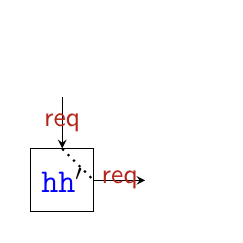
\begin{tikzpicture}[node distance=1.5cm,scale=1]
        \node (square-h) [draw,minimum width=0.8cm,minimum height=0.8cm] {\large $\hh\hh'$};
        \node [state] (h-a) [above of = square-h, draw=none] {};
        \draw [-stealth] (h-a) --  node {$\msg[req]$} (square-h);
        \node [state] (k-a) [right of = square-h, draw=none] {};
        \draw [-stealth] (square-h) --  node {$\msg[req]$} (k-a);
        %
        \draw (0,0.4)[dotted,thick]  --  (0.4,0); % carrying a inside h  
 \end{tikzpicture}
 \hspace{2mm}
        }
 $
 \caption{\label{fig:onegwcomp} Single-gateway composition of $S_1$ and $S_2$.}
 }
\end{figure}

\noindent
The dotted line crossing the participant $\hh\hh'$ represents the fact that it works just as  forwarder:
a message $\msg[req]$ sent to $\hh$  by either $\ttr$ or $\ttr'$, is now sent to $\hh\hh'$
which immediately forwards it to $\tts$.
This sort of composition, however, would not be quite conservative.
In fact, in $\ttr$  the name $\hh$ as receiver of the message
  $\msg[req]$ should now be replaced by $\hh\hh'$, whereas  in $\tts$ the name $\hh'$ as sender of the message  $\msg[req]$ should now be replaced by $\hh\hh'$\footnote{
Notice that a {\em direct} composition -- where interface are taken out and  $\msg[req]$
is sent by either $\ttr$ or $\ttr'$ directly to $\tts$ -- would be even less conservative.
Besides, as discussed in~\cite{BdLH19}, several further problems would arise.
In~\cite{BDLT21} direct composition is actually implemented in the setting of MultiParty Session Types at the cost of fairly strong requirements.
}. 
To get a more conservative composition, in~\cite{BdLH19} $\hh$ and $\hh'$ are
replaced by forwarders (that we dub ``gateways'') preserving the very same names.
The gateway for $\hh$ now forwards to the gateway for $\hh'$ the $\msg[req]$ received from either 
$\ttr$ or $\ttr'$, whereas the gateway for $\hh'$ forwards it to $\tts$, as depicted in \cref{fig:bincomp}.  
\begin{figure}[h]
    \centering{\small
    $
\begin{array}{l}
\text{\large $S_1$}\!\mathtt{comp}\text{\large $S_2$}\\[22mm]
\end{array}
 \dbox{ \hspace{28mm}
 \begin{tikzpicture}[node distance=1.5cm,scale=1]
        \node (square-h) [draw,minimum width=0.8cm,minimum height=0.8cm] {\large $\hh$};
        \draw [-stealth] (h-a) --  node {$\msg[req]$} (square-h);
        \node (square-k) [draw,minimum width=0.8cm,minimum height=0.8cm, right of = square-h, xshift=5mm] {\large $\hh'$};
        \node [state] (k-a) [right of = square-k, draw=none] {};
         \node[draw=none,fill=none] (phantom) [above = 12mm  of square-h]{};
        \draw [-stealth] (square-k) --  node [above]{$\msg[req]$} (k-a);
        %
        \draw (0,0.4)[dotted,thick]  --  (0.4,0); % carrying a inside h  
        \draw [-stealth] (0.4,0)  -- node [above] {$\msg[req]$} (1.6,0); % carrying a from h to k
        \draw (1.6,0)[dotted,thick]  --  (2.4,0); % carrying a inside k
 \end{tikzpicture}
 \hspace{4mm}
        }
 $
 \caption{\label{fig:bincomp} The PaI idea for binary composition via gateways}
 }
\end{figure}

 It is worth remarking that the above sketched PaI approach to binary composition does not expect any particular condition to be satisfied by a single participant in order to be used as an interface:
 any participant of a system can be looked at as an interface as far as it is possible to find
a  complementary participant in another system. 
Both conservativity and flexibility are features of the PaI composition idea.
 Conservativity holds since all participants not acting as interfaces remain untouched whereas flexibility holds since, in principle, any participant can play the role of an interface. This fact is independent of the particular formalism used for protocol descriptions and system designs/implementations. 
{\em Safety}, instead, can be checked  only once we take into account a
concrete behavioral instantiation, namely a specific formalism.
In~\cite{BdLH19} such a check was carried out in the formalism of Communicating Finite State Machines  (CFSM)~\cite{BZ83},
where participants' behaviours are described in terms of automata with edges labelled with
either input or output actions. Such actions concern messages asynchronously exchanged 
by means of unbounded FIFO queues (one for each pair of participants).
In such a setting, the abstract example we used above to introduce the very general idea
of PaI composition can be made more specific: the two interfaces of $S_1$ and $S_2$ could be
as in \cref{fig:cfsminterfaces}, where $\ain[r][h][][req]$ and $\ain[r'][h][][req]$ denote $\hh$'s actions of reading a message $\msg[req]$, if any, respectively from the queues $\ttr\hh$
and $\ttr'\hh$ (we do not show queues in these introductory figures) which enable the asynchronous message exchanges from $\ttr$ to $\hh$ and from $\ttr'$ to $\hh$.
Label $\aout[h'][s][][req]$ 
denotes instead $\hh'$'s action of inserting a message $\msg[req]$ 
in the queue $\hh'\tts$.
Notice hence that, by the above interpretation of labels, messages $\msg[req]$
are asynchronously received by $\hh$ alternately from $\ttr$ and $\ttr'$.
In $S_2$, instead,  $\hh'$ keeps on asynchronously and indefinitely 
sending  messages $\msg[req]$ to $\tts$. 

 \begin{figure}[h]
    \centering{\small
    $
\raisebox{12mm}{\text{\large $S_1\,\,$}}
    \dbox{
\hspace{24mm}
     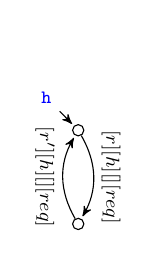
\begin{tikzpicture}[mycfsm]
      %\tikzstyle{every edge}=[carrow]
      % 
      \node[state] (zero) {$~$};
      \node[state] (one) [below of=zero,yshift=5mm]   {$~$};
      \node[draw=none,fill=none] (start) [above left = 0.3cm  of zero]{$\HH$};
      \node[draw=none,fill=none] (phantom) [above = 12mm  of zero]{};
      % 
      \path
      (start) edge node {} (zero) 
      (zero) edge[bend left] node[above] {$\ain[r][h][][req]$} (one)
      (one) edge[bend left] node[below] {$\ain[r'][h][][req]$} (zero)
      ;
  \end{tikzpicture}
            }
\hspace{12mm}
     \dbox{
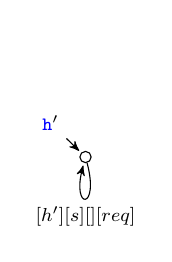
\begin{tikzpicture}[mycfsm]
		  % 
		  \node[state] (zero) {$~$};
		  \node[draw=none,fill=none] (start) [above left = 0.3cm  of zero]{$\hh'$};
             \node[draw=none,fill=none] (phantom) [above = 16mm  of zero]{};
		  % 
		  \path
            (start) edge node {} (zero) 
		  (zero) edge [loop below,looseness=40] node[below] {$\aout[h'][s][][req]$} (zero)
		  ;
		\end{tikzpicture}\qquad\qquad
             }
 \raisebox{12mm}{\text{\large $\,\,S_2$}}
 $\vspace{-2mm}
 \caption{\label{fig:cfsminterfaces} Two CFSM interfaces.}
 }
\end{figure}

\noindent
The binary PaI composition of $S_1$ and $S_2$ via gateways, using the communicating machines 
$\hh$ and $\hh'$, is hence as in \cref{fig:bpaicfscomp},
where the gray nodes are introduced by the gateway construction.


\begin{figure}[h]
    \centering{\small
    $
    \begin{array}{l}
\text{\large $S_1$}\!\mathtt{comp}\text{\large $S_2$}\\[22mm]
\end{array}
\dbox{
            \quad\qquad\qquad\qquad 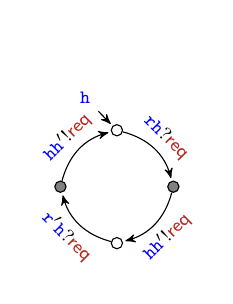
\begin{tikzpicture}[mycfsm]
  \node[state]           (0)                        {$~$};
  \node[state]           (hat0)          [below left of=0, yshift=5mm, fill=gray,xshift=5mm]              {$~$};
  \node[draw=none,fill=none] (phantom) [above = 12mm  of 0]{};
   \node[draw=none,fill=none] (start) [above left = 0.3cm  of 0]{$\HH$};
  \node[state]            (1) [below right of=hat0, yshift=5mm,xshift=-5mm] {$~$};
  \node[state]           (hat0') [below right of=0, yshift=5mm, fill=gray,xshift=-5mm] {$~$};

   \path  (start) edge node {} (0) 
            (hat0)     edge   [bend left]        node [above] {${\hh\hh'}!{\msg[req]}$} (0)
             (0)        edge   [bend left]      node [above]  {${\ttr\hh}?{\msg[req]}$} (hat0')
             (1)        edge  [bend left]         node [below] {${\ttr'\hh}?{\msg[req]}$} (hat0)
             (hat0')  edge  [bend left]      node [below] {${\hh\hh'}!{\msg[req]}$} (1);       
             \end{tikzpicture}
\hspace{4mm}
\begin{tikzpicture}[mycfsm]
      %\tikzstyle{every edge}=[carrow]
      % 
      \node[state] (zero) [yshift=-4mm] {$~$};
      \node[state] (one) [below of=zero, fill=gray,yshift=5mm]   {$~$};
      \node[draw=none,fill=none] (phantom) [above = 10mm  of 0]{};
      \node[draw=none,fill=none] (start) [above left = 0.3cm  of zero]{$\hh'$};
      % 
      \path
      (start) edge node {} (zero) 
      (zero) edge[bend left] node[below] {$\ain[h][h'][][req]$} (one)
      (one) edge[bend left] node[above] {$\aout[h'][s][][req]$} (zero)
      ;
 \end{tikzpicture}\qquad\qquad 
 }
 $
 \caption{\label{fig:bpaicfscomp} Binary PaI composition of CFSM systems.}
 }
\end{figure}



For CFSM the generic idea of complementarity was formalised in~\cite{BdLH19} in terms of
a {\em compatibility} relation.
Roughly, two participants are compatible whenever, in case the first is able to receive a message, 
the latter is able to send a similar message.
In a sense, abstracting from the (local) names of senders and receivers, their traces of
messages are dual, namely obtained one from the other by interchanging the input/output tags. 
% The graphics in~\cref{fig:bincomp} illustrates the PaI idea for the binary case.
%  In that abstract representation of the participants' behaviours, only the possibility of 
% sending/receiving messages is actually represented. 
Preservation by composition of a whole bunch of communication properties was proven in~\cite{BdLH19}
under the compatibility requirement of interfaces.
It is natural hence to wonder whether weaker requirements can be taken into account
depending on the particular property whose preservation by composition we wish to obtain.
We shall indirectly give an answer to such a question in the more general case of multicomposition,
where also more than two participants can be composed using the PaI approach.
We define multicompostion in terms of {\em connection policies} (roughly, descriptions -- in terms of CFSM systems -- of how the gateways forward messages among themselves and possible orchestrators, see \cref{sec:opensys}). Our main result is %safety for PaI multicomposition, i.e. we prove 
that many properties are preserved by multicomposition under the requirement that
the same property is enjoyed by the connection policy the composition depends on. 
The notion of connection policy is rather pleonastic in the case of binary composition since, given two interfaces, their corresponding connection policy is uniquely determined.  
Binary connection policies can however be useful as a smooth introduction to their multicomposition
version.
As hinted before, a connection policy is a CFSM system describing how the messages
from/to the interfaces have to be forwared by the gateways implementing the composition.
For the interfaces of \cref{fig:cfsminterfaces}, the (unique) connection policy would be
the two-participant system $\cs$ on the left of \cref{fig:abcm}.
Here and later on in the technical part of the paper, we use a dotted notation in order to
link a connection policy participant to its corresponding interface. 
By considering instead only static aspects of the machines -- i.e. by abstracting from dynamic issues like   
the logical order of the exchanged messages -- we get the box-and-arrow drawing on the right of 
\cref{fig:abcm}, corresponding to the (binary) connection model $\cm$ complying with the connection policy $\cs$.
 \begin{figure}[h]
    \centering{\small
    $
 \raisebox{10mm}{\text{\normalsize $\cs\,\,$}}
    \dbox{\hspace{-2mm}
     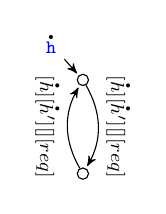
\begin{tikzpicture}[mycfsm]
      %\tikzstyle{every edge}=[carrow]
      % 
      \node[state] (zero) {$~$};
      \node[state] (one) [below of=zero,yshift=5mm]   {$~$};
      \node[draw=none,fill=none] (start) [above left = 0.3cm  of zero]{$\dot\HH$};
      % 
      \path
      (start) edge node {} (zero) 
      (zero) edge[bend left] node[above] {$\aout[\dot{h}][\dot{h}'][][req]$} (one)
      (one) edge[bend left] node[below] {$\aout[\dot{h}][\dot{h}'][][req]$} (zero)
      ;
  \end{tikzpicture}         
%\hspace{2mm}
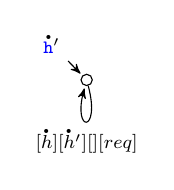
\begin{tikzpicture}[mycfsm]
		  % 
		  \node[state] (zero) {$~$};
		  \node[draw=none,fill=none] (start) [above left = 0.3cm  of zero]{$\dot\hh'$};
		  % 
		  \path
            (start) edge node {} (zero) 
		  (zero) edge [loop below,looseness=40] node[below] {$\ain[\dot{h}][\dot{h}'][][req]$} (zero)
		  ;
		\end{tikzpicture} \hspace{-2mm}
             }
 $
 \hspace{32mm}
 $
    \dbox{
 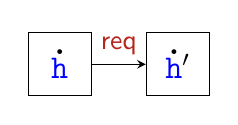
\begin{tikzpicture}[node distance=1.5cm,scale=1]
        \node (square-h) [draw,minimum width=0.8cm,minimum height=0.8cm] {\large $\dot\hh$};
        \node (square-k) [draw,minimum width=0.8cm,minimum height=0.8cm,right of = square-h] {\large $\dot\hh'$};
       \draw [-stealth] (square-h) --  node [above] {$\msg[req]$} (square-k);
 \end{tikzpicture} 
             }
 \raisebox{5mm}{\text{\normalsize $\,\,\cm$}}
 $
 \vspace{-2mm}
 \caption{\label{fig:abcm} A binary connection policy $\cs$  (left) and a binary connection model $\cm$ (right).}
 }
\end{figure}

In the multicomposition case, a connection policy is necessary to construct gateways out of
the interface participants since, unlike the present case, more then two systems can be present. 

% A connection model, instead, focuses on the architectural aspect of the composition in a formalism-independent way. Our safety result for PaI multicomposition will be independent from the connection model statically describing the connection policy on which a multicomposition is based.
%Nonetheless we deem the notion of connection model worth formalising (see  \label{def:cm}) and its interest will be discussed throughout the paper.

Our safety result for multicomposition entails that, in case we were interested just in the
reception-error freedom preservation (\cref{def:safeness}), we could safely compose 
two reception-error free $S_1$ and $S_2$ system also when we had the two {\em non compatible} 
interface CFSMs of \cref{fig:othercfsminterfaces}.
%, whose corresponding connection policy is however reception-error free.
\begin{figure}[h!]
    \centering{\small
    $
\raisebox{12mm}{\text{\large $S_1\,\,$}}
    \dbox{
\hspace{24mm}
     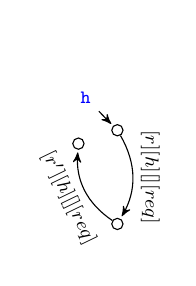
\begin{tikzpicture}[mycfsm]
      %\tikzstyle{every edge}=[carrow]
      % 
      \node[state] (zero) {$~$};
      \node[state] (one) [below of=zero,yshift=5mm]   {$~$};
       \node[state] (two) [left=4mm of zero,yshift=-2mm]   {$~$};
      \node[draw=none,fill=none] (start) [above left = 0.3cm  of zero]{$\HH$};
      \node[draw=none,fill=none] (phantom) [above = 12mm  of zero]{};
      % 
      \path
      (start) edge node {} (zero) 
      (zero) edge[bend left] node[above] {$\ain[r][h][][req]$} (one)
      (one) edge[bend left] node[below] {$\ain[r'][h][][req]$} (two)
      ;
  \end{tikzpicture}
            }
\hspace{12mm}
     \dbox{
%\begin{tikzpicture}[mycfsm]
%		  % 
%		  \node[state] (zero) {$~$};
%		  \node[draw=none,fill=none] (start) [above left = 0.3cm  of zero]{$\kk$};
%		  \node[state] (one) [below = of zero, yshift=8mm]{$~$};
%             \node[draw=none,fill=none] (phantom) [above = 16mm  of zero]{};
%		  % 
%		  \path
%            (start) edge node {} (zero) 
%		  (zero) edge node[below] {$\aout[k][s][][req]$} (one)
%		  ;
%		\end{tikzpicture}
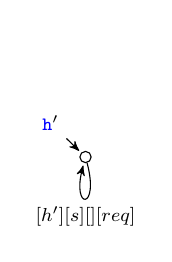
\begin{tikzpicture}[mycfsm]
		  % 
		  \node[state] (zero) {$~$};
		  \node[draw=none,fill=none] (start) [above left = 0.3cm  of zero]{$\hh'$};
             \node[draw=none,fill=none] (phantom) [above = 16mm  of zero]{};
		  % 
		  \path
            (start) edge node {} (zero) 
		  (zero) edge [loop below,looseness=40] node[below] {$\aout[h'][s][][req]$} (zero)
		  ;
\end{tikzpicture}\qquad\qquad
             }
 \raisebox{12mm}{\text{\large $\,\,S_2$}}
 $\vspace{-2mm}
 \caption{\label{fig:othercfsminterfaces} Two other CFSM interfaces.}
 }
\end{figure}
After \cref{sec:opensys} the reader can turn back to \cref{fig:othercfsminterfaces} and check, as a simple exercise,
that the (unique) connection policy induced by $\hh$ and $\hh'$ is reception-error free but not deadlock-free.\\

We now briefly introduce the notion of {\em orchestrated} PaI composition for the binary case as 
an introductory foretaste to its multicomposition version.
Let us hence go back to the composition example of \cref{fig:bpaicfscomp} and assume that
we would like message $\msg[req]$ -- the one that drives the substance diffusion -- 
to actually reach gateway $\hh'$ only in case some particular conditions are met (say, absence of too high temperature).
It is of course possible to redefine the gateways so that the above check be carried out by one or both of them. However, doing so would contrast with the
separation of concerns (SoC, a fundamental principle in software engineering) and would make the
composed systems less loosely coupled.
We could hence have a specific {\em orchestrating} participant (or a set of participants) to perform the temperature check, so separating that task from the forwarding one needed for the composition. 
In our example, an orchestrating participant would look as in \cref{fig:orchcfscomp},
where the participant $\tto$ can internally choose whether ignoring a message $\msg[req]$ or not.
\begin{figure}[h]
    \centering{\small
    $
    \begin{array}{l}
\text{\large $S_1$}\!\mathtt{orch\text{-}comp}\text{\large $S_2$}\\[30mm]
\end{array}
\dbox{
            \qquad\qquad\qquad\qquad 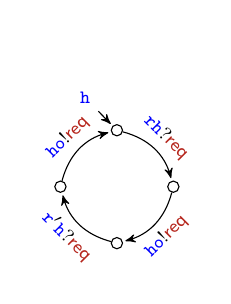
\begin{tikzpicture}[mycfsm]
  \node[state]           (0)                        {$~$};
  \node[state]           (hat0)          [below left of=0, yshift=5mm, xshift=5mm]              {$~$};
  \node[draw=none,fill=none] (phantom) [above = 12mm  of 0]{};
   \node[draw=none,fill=none] (start) [above left = 0.3cm  of 0]{$\HH$};
  \node[state]            (1) [below right of=hat0, yshift=5mm,xshift=-5mm] {$~$};
  \node[state]           (hat0') [below right of=0, yshift=5mm, xshift=-5mm] {$~$};

   \path  (start) edge node {} (0) 
            (hat0)     edge   [bend left]        node [above] {${\hh\tto}!{\msg[req]}$} (0)
             (0)        edge   [bend left]      node [above]  {${\ttr\hh}?{\msg[req]}$} (hat0')
             (1)        edge  [bend left]         node [below] {${\ttr'\hh}?{\msg[req]}$} (hat0)
             (hat0')  edge  [bend left]      node [below] {${\hh\tto}!{\msg[req]}$} (1);       
             \end{tikzpicture}
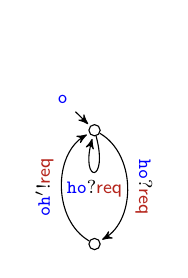
\begin{tikzpicture}[mycfsm]
  \node[state]           (0)                        {$~$};
  \node[draw=none,fill=none] (phantom) [above = 12mm  of 0]{};
   \node[draw=none,fill=none] (start) [above left = 0.3cm  of 0]{$\tto$};
  \node[state]           (hat0') [below of = 0, yshift=2mm] {$~$};

   \path  (start) edge node {} (0) 
             (0)        edge   [bend left= 60]      node [above]  {${\hh\tto}?{\msg[req]}$} (hat0')
             (hat0')  edge  [bend left= 60]      node [above] {${\tto\hh'}!{\msg[req]}$} (0)
              (0) edge [loop below,looseness=40] node[below] {${\hh\tto}?{\msg[req]}$} (0);       
             \end{tikzpicture}
\begin{tikzpicture}[mycfsm]
      %\tikzstyle{every edge}=[carrow]
      % 
      \node[state] (zero) [yshift=-4mm] {$~$};
      \node[state] (one) [below of=zero, yshift=5mm]   {$~$};
      \node[draw=none,fill=none] (phantom) [above = 10mm  of 0]{};
      \node[draw=none,fill=none] (start) [above left = 0.3cm  of zero]{$\hh'$};
      % 
      \path
      (start) edge node {} (zero) 
      (zero) edge[bend left] node[below] {$\ain[o][h'][][req]$} (one)
      (one) edge[bend left] node[above] {$\aout[h'][s][][req]$} (zero)
      ;
 \end{tikzpicture}\qquad\qquad 
 }
 $
 \caption{\label{fig:orchcfscomp} An orchestrated binary PaI composition of CFSM systems.}
 }
\end{figure}

\noindent
The notions of connection model and connection policy naturally extend to the orchestration case.
For our simple example, the connection model and connection policy would be as in \cref{fig:orchbcm}
 \begin{figure}[h]
    \centering{\small
    $
 \raisebox{10mm}{\text{\normalsize $\cs^o\,\,$}}
    \dbox{ \hspace{-2mm}
     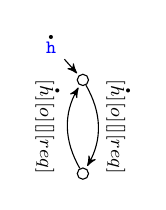
\begin{tikzpicture}[mycfsm]
      %\tikzstyle{every edge}=[carrow]
      % 
      \node[state] (zero) {$~$};
      \node[state] (one) [below of=zero,yshift=5mm]   {$~$};
      \node[draw=none,fill=none] (start) [above left = 0.3cm  of zero]{$\dot\HH$};
      % 
      \path
      (start) edge node {} (zero) 
      (zero) edge[bend left] node[above] {$\aout[\dot{h}][o][][req]$} (one)
      (one) edge[bend left] node[below] {$\aout[\dot{h}][o][][req]$} (zero)
      ;
  \end{tikzpicture}         
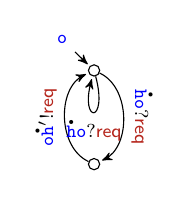
\begin{tikzpicture}[mycfsm]
  \node[state]           (0)                        {$~$};
   \node[draw=none,fill=none] (start) [above left = 0.3cm  of 0]{$\tto$};
  \node[state]           (hat0') [below of = 0, yshift=5mm] {$~$};

   \path  (start) edge node {} (0) 
             (0)        edge   [bend left= 65]      node [above]  {${\dot\hh\tto}?{\msg[req]}$} (hat0')
             (hat0')  edge  [bend left= 65]      node [above] {${\tto\dot\hh'}!{\msg[req]}$} (0)
              (0) edge [loop below,looseness=40] node[below] {${\dot\hh\tto}?{\msg[req]}$} (0);       
             \end{tikzpicture}
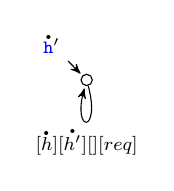
\begin{tikzpicture}[mycfsm]
		  % 
		  \node[state] (zero) {$~$};
		  \node[draw=none,fill=none] (start) [above left = 0.3cm  of zero]{$\dot\hh'$};
		  % 
		  \path
            (start) edge node {} (zero) 
		  (zero) edge [loop below,looseness=40] node[below] {$\ain[\dot{h}][\dot{h'}][][req]$} (zero)
		  ;
		\end{tikzpicture}\hspace{-2mm}
             }
 $
 \hspace{28mm}
 $
    \dbox{
 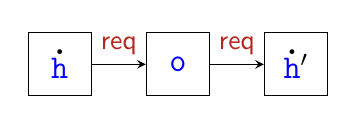
\begin{tikzpicture}[node distance=1.5cm,scale=1]
        \node (square-h) [draw,minimum width=0.8cm,minimum height=0.8cm] {\large $\dot\hh$};
         \node (square-o) [draw,minimum width=0.8cm,minimum height=0.8cm,right of = square-h] {\large $\tto$};
        \node (square-k) [draw,minimum width=0.8cm,minimum height=0.8cm,right of = square-o] {\large $\dot\hh'$};
       \draw [-stealth] (square-h) --  node [above]{$\msg[req]$} (square-o);
       \draw [-stealth] (square-o) --  node [above] {$\msg[req]$} (square-k);
 \end{tikzpicture} 
             }
 \raisebox{5mm}{\text{\normalsize $\,\,\cm^o$}}
 $
 \vspace{-2mm}
 \caption{\label{fig:orchbcm} Binary orchestrated connection policy (left) and connection model (right).}
 }
\end{figure}

\noindent
As discussed later on, all the above orchestration-related notions naturally extend to the multicomposition case, as well as to the case with multiple orchestrating participants.\\


Safety of binary PaI composition was investigated in~\cite{BdLH19}  for standard CFSM 
and in~\cite{BLT20,BLP22b,BLT23} for a synchronous version of CFSM.  
 
Safety of binary PaI composition was investigated in~\cite{BDLT21} for the synchronous 
version of another relevant formalism for the description and verification of concurrent communicating systems, namely
MultiParty Session Types  (MPST)~\cite{HYC08,Honda2016}. 

 



%into coupled forwarders (gateways), provided these participants 
%So, a composition can be carried on if the choosen interfaces are ``complementary''.





%participants exhibit ``compatible'' behaviours. 

 
 
 
 
%If interface participant $\HH$ of the first system $S_1$
%can receive a message $\msg[a]$  from some participant of $S_1$ and interface participant $\KK$
% of the second system $S_2$ can send $\msg[a]$ to some participant of $S_2$,  then the gateway replacing the first interface (also called $\HH$) will forward the received message to the gateway for $\KK$. 



% Roughly, two participants are compatible whenever, in case the first is able to receive a message, 
%the latter is able to send a similar message.
%In a sense, abstracting from the (local) names of senders and receivers, their traces of
%messages are dual, namely obtained one from the other by interchanging the input/output tags.  
% The graphics in~\cref{fig:bincomp} illustrates the PaI idea for the binary case.
 
 
 
 
 
%If interface participant $\HH$ of the first system $S_1$
%can receive a message $\msg[a]$  from some participant of $S_1$ and interface participant $\KK$
% of the second system $S_2$ can send $\msg[a]$ to some participant of $S_2$,  then the gateway replacing the first interface (also called $\HH$) will forward the received message to the gateway for $\KK$. 


  
%\begin{figure}[t]
%    \centering{\small
%    \vspace{-14mm}
%    $
%    \begin{array}{@{\hspace{-10mm}}c@{\hspace{-10mm}}}
% \begin{tikzpicture}[node distance=1.5cm,scale=1]
%        \node (square-h) [draw,minimum width=0.8cm,minimum height=0.8cm] {\large $\hh$};
%        \node [state] (h-a) [above of = square-h, draw=none] {};
%        \node [state] (h-c) [left of = square-h, draw=none] {};
%        \draw [-stealth] (h-a) --  node {$\msg[a]$} (square-h);
%        %\draw [-stealth] (square-h) --  node {$\msg[c]$} (h-c);
% \end{tikzpicture}
%\hspace{8mm}
%\begin{array}{c}
%\\[10mm]
%| \\
%| \\
%| \\
%|
%\end{array}
% \hspace{8mm}
% \begin{tikzpicture}[node distance=1.5cm,scale=1]
%        \node (square-k) [draw,minimum width=0.8cm,minimum height=0.8cm] {\large $\KK$};
%        \node [state] (k-b) [above of = square-k, draw=none] {};
%        \node [state] (k-a) [right of = square-k, draw=none] {};
%        %\draw [-stealth] (k-b) --  node {$\msg[b]$} (square-k);
%        \draw [-stealth] (square-k) --  node {$\msg[a]$} (k-a);
% \end{tikzpicture}
%  \end{array}
%  \qquad
%  \begin{array}{c}
%  \\[8mm]
%  \text{becomes}
%  \end{array}
%  \qquad
%  \begin{array}{c}
%  \\[6mm]
%  \begin{tikzpicture}[node distance=1.5cm,scale=1]
%        \node (square-h) [draw,minimum width=0.8cm,minimum height=0.8cm] {\large $\hh$};
%        \draw [-stealth] (h-a) --  node {$\msg[a]$} (square-h);
%        \node (square-k) [draw,minimum width=0.8cm,minimum height=0.8cm, right of = square-h, xshift=5mm] {\large $\KK$};
%        \node [state] (k-a) [right of = square-k, draw=none] {};
%        \draw [-stealth] (square-k) --  node {$\msg[a]$} (k-a);
%        %
%        \draw (0,0.4)[dotted,thick]  --  (0.4,0); % carrying a inside h  
%        \draw [-stealth] (0.4,0)  -- node {$\msg[a]$} (1.6,0); % carrying a from h to k
%        \draw (1.6,0)[dotted,thick]  --  (2.4,0); % carrying a inside k
% \end{tikzpicture}
% \end{array}
% $\vspace{-2mm}
% \caption{\label{fig:bincomp} The PaI idea for binary composition via gateways}
% }
%\end{figure}

%\brc Not sure whether we need this paragraph. The comparison is already explained above directly
%when the Contributions paragraph starts. I wouldn't know what to say otherwise. \erc
% Such a paragraph is however needed, since the editors wrote:
%``In accordance with the JLAMP editorial policies, we would appreciate it if your submission includes a clear statement of the novelty with  respect to the work presented at ICE.'' 
 
\noindent
\paragraph{The PaI Approach to Multicomposition}
\label{sec:pai-multicomp}
The PaI approach to multicomposition has been exploited in~\cite{BDGY23}
for synchronous MPST, whereas in the present paper 
we investigate it for (asynchronous) CFSM with the possible  presence of \emph{orchestrating participants}.
In order to incrementally illustrate the idea underlying \emph{PaI
  orchestrated multicomposition}, we put aside for the moment the notion of orchestration
and consider an example from~\cite{BDGY23} having four systems $S_1$,  $S_2$, $S_3$ and $S_4$.
As shown in~\cref{fig:four-ips}, we have selected for each system one participant
as an interface, named respectively $\hh_1$, $\hh_2$, $\hh_3$ and $\hh_4$.
 
%\begin{wrapfigure}{r}{0.45\textwidth}
\begin{figure}[h]
    %\vspace{-8mm}
     \centering{\small
    $
    \begin{array}{@{\hspace{0mm}}c@{\hspace{-2mm}}}
    \begin{array}{c@{\hspace{-2mm}}c}
    \text{\large $S_1$}
    &
 \begin{tikzpicture}[node distance=1.5cm,scale=1]
        \node (square-h) [draw,minimum width=0.8cm,minimum height=0.8cm] {\large $\hh_1$};
        \node [state] (h-a) [above of = square-h, draw=none] {};
        \node [state] (h-c) [left of = square-h, draw=none] {};
        \draw [-stealth] (h-a) --  node {$\msg[a]$} (square-h);
        \draw [-stealth] (square-h) --  node {$\msg[c]$} (h-c);
 \end{tikzpicture}
 \end{array}
 \hspace{4mm}
\begin{array}{c}
 \\
 \\
| \\
| \\
|\\
|\\
\end{array}
 \hspace{4mm}
 \begin{array}{c@{\hspace{-2mm}}c}
\begin{tikzpicture}[node distance=1.5cm,scale=1]
        \node (square-k) [draw,minimum width=0.8cm,minimum height=0.8cm] {\large $\hh_2$};
        \node [state] (k-b) [above of = square-k, draw=none] {};
        \node [state] (k-a) [right of = square-k, draw=none] {};
        \draw [-stealth] (k-b) --  node {$\msg[b]$} (square-k);
        \draw [-stealth] (square-k) --  node {$\msg[a]$} (k-a);
 \end{tikzpicture}
 &
 \text{\large $S_2$} 
 \end{array}
 \\[12mm]
\hspace{3mm}- - - -    \hspace{8mm}- - - - -  \\[-5mm]
\begin{array}{@{\hspace{0mm}}c@{\hspace{0mm}}c}
\\[4mm]
\text{\large $S_3\hspace{-2mm}$} 
&
 \begin{tikzpicture}[node distance=1.5cm,scale=1]
        \node (square-v) [draw,minimum width=0.8cm,minimum height=0.8cm] {\large $\hh_3$};
        \node [state] (v-b) [left of = square-v, draw=none] {};
        \node [state] (v-a) [below of = square-v, draw=none] {};
        \draw [-stealth] (v-a) --  node {$\msg[a]$} (square-v);
        \draw [-stealth] (square-v) --  node {$\msg[b]$} (v-b);
 \end{tikzpicture}
 \end{array}
 \hspace{4mm}
\begin{array}{c}
 \\[-8mm]
| \\
| \\
| \\
|
\end{array}
 \hspace{4mm}
 \begin{array}{c@{\hspace{-2mm}}}
 \\[-6mm]
 \begin{tikzpicture}[node distance=1.5cm,scale=1]
        \node (square-w) [draw,minimum width=0.8cm,minimum height=0.8cm] {\large $\hh_4$};
        \node [state] (w-c) [right of = square-w, draw=none] {};
        \node [state] (w-a) [below of = square-w, draw=none] {};
        \node [state] (w-b) [above right of = square-w, draw=none] {};
        \draw [-stealth] (w-c) --  node {$\msg[c]$} (square-w);
        \draw [-stealth] (square-w) --  node {$\msg[a]$} (w-a);
        \draw [stealth-] (square-w) --  node {$\msg[b]$} (w-b);
 \end{tikzpicture}
 \hspace{-6mm}
 \begin{array}{l}
 \\[6mm]
 \text{\large\ \ $S_4$}
 \end{array} 
 \end{array}
 \\[-4mm]
 \end{array}
 $
 }
\caption{\label{fig:four-ips}
Four systems with their respective interface participants}
 \end{figure}
% \vspace{-5mm}
% \end{wrapfigure}
As in~\cref{fig:bincomp}, we begin by considering only static aspects, i.e. we abstract from dynamic issues like the logical order of the exchanged messages, whose representation depends, instead, on the chosen formalism (CFSM in the present paper).



 For what concerns  our example of \cref{fig:four-ips},
 one could decide that message $\msg[a]$ received by $\hh_1$ has 
 to be forwarded
 to $\hh_4$; the $\msg[a]$ received by $\hh_3$
 to $\hh_2$; the $\msg[b]$ received by $\hh_2$ 
 or by $\hh_4$ to $\hh_3$; 
 the $\msg[c]$ received by $\hh_4$ to $\hh_1$.
 Another possible choice %(see policy B  in Figure~\ref{fig:twocm})) 
could be similar to the previous one but for the forwarding
of the messages $\msg[a]$: the one received by $\HH_1$ could be forwarded now to $\hh_2$
whereas the one received by $\hh_3$ could be forwarded to $\hh_4$. 
 Such different ``choices of partners'' can be represented 
 by the {\em connection models} $\cm_\mathrm{A}$ and $\cm_\mathrm{B}$ in \cref{fig:choicesAB} (we now avoid enclosing systems within dashed squares).
  
As previously mentioned, dotted names are used for ``virtual'' participants whose behaviours  represent 
 the forwarding policies of their undotted counterparts.
 

%%% CONNECTION MODELS
 \begin{figure}[ht]
    \centering{
    \raisebox{15mm}{$\cm_\mathrm{A}$}
    $\begin{array}{c@{\qquad\qquad\qquad\qquad\qquad}c}
 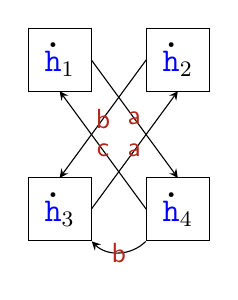
\begin{tikzpicture}[node distance=1.5cm,scale=1]
        \node (square-h) [draw,minimum width=0.8cm,minimum height=0.8cm] {\large $\dot\hh_1$};
        \node (square-k) [draw,minimum width=0.8cm,minimum height=0.8cm, right of = square-h] {\large $\dot\hh_2$};
        \node (square-v)  [draw,minimum width=0.8cm,minimum height=0.8cm, below of = square-h, yshift=-4mm] {\large $\dot\hh_3$};
        \node (square-w)  [draw,minimum width=0.8cm,minimum height=0.8cm, below of = square-k, yshift=-4mm] {\large $\dot\hh_4$};
        \draw[-stealth]  (square-w) to[out=-135,in=-45]  node {$\msg[b]$} (square-v);
        %
        %
        \draw [-stealth] (0.4,0)  -- node {$\msg[a]$}  (1.5,-1.5 ); % carryng a from h to w    
         \draw [stealth-] (0,-0.4)  -- node {$\msg[c]$} (1.1,-1.9); % carryng c from w to h 
        \draw [-stealth] (0.4,-1.9)  --  node {$\msg[a]$} (1.5,-0.4 ); % carrying a from v to k
        \draw [stealth-] (0,-1.5)  --  node {$\msg[b]$} (1.1,0); % carrying  b from k to v
 \end{tikzpicture}
&
 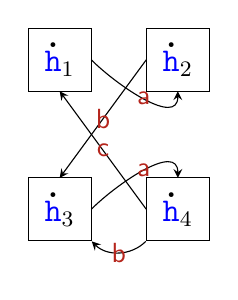
\begin{tikzpicture}[node distance=1.5cm,scale=1]
        \node (square-h) [draw,minimum width=0.8cm,minimum height=0.8cm] {\large $\dot\HH_1$};
        \node (square-k) [draw,minimum width=0.8cm,minimum height=0.8cm, right of = square-h] {{\large $\dot\hh_2$}};
        \node (square-v)  [draw,minimum width=0.8cm,minimum height=0.8cm, below of = square-h, yshift=-4mm] {{\large $\dot\hh_3$}};
        \node (square-w)  [draw,minimum width=0.8cm,minimum height=0.8cm, below of = square-k, yshift=-4mm] {{\large $\dot\hh_4$}};
        %
        \draw [-stealth] (square-w) to[out=-135,in=-45]  node {$\msg[b]$} (square-v);
        %
        %
        \draw [-stealth] (0.4,-1.9) to[out=45,in=90] node {$\msg[a]$} (1.5,-1.5 ); % carryng a from v to w    
         \draw [stealth-] (0,-0.4)  -- node {$\msg[c]$} (1.1,-1.9) ; % carryng c from w to h 
        \draw [-stealth]  (0.4,0)  to[out=-45,in=-90]  node {$\msg[a]$} (1.5,-0.4 ); % carrying a from h to k
        \draw [stealth-] (0,-1.5)  --  node {$\msg[b]$} (1.1,0); % carrying  b from k to v
 \end{tikzpicture}
 \raisebox{14.5mm}{$\,\,\,\,\cm_\mathrm{B}$}
% \\
% \begin{array}{c}
%  \\[1mm]
% (\text{Choice A})
% \end{array}&
% \begin{array}{c}
% \\[1mm]
% (\text{Choice B})
% \end{array}
 \end{array}
 $
 }
 \caption{\label{fig:choicesAB} Two connection models for multicomposition.}\label{fig:twocm}
 \end{figure}
 
 \noindent
 The  architecture  of the resulting composed systems, according to the connection models is
represented  by the diagrams  in~\cref{fig:multiconnection},  where the names $\hh_1, \hh_2, \hh_3$
and $\hh_4$ now represent gateways.
\begin{figure}[h]%{c}{0.6\textwidth}
\vspace{-4mm}
    \centering{
    $\begin{array}{c@{\quad\qquad}c}
 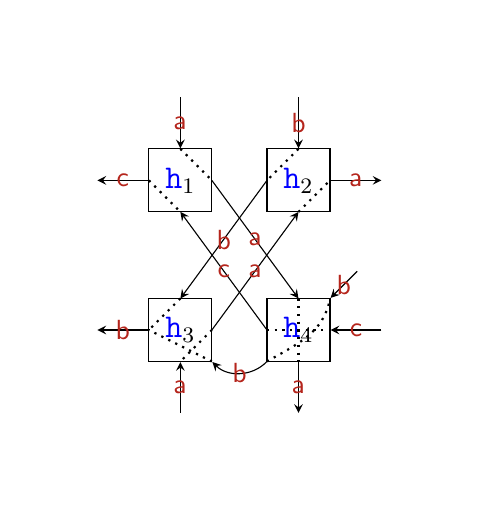
\begin{tikzpicture}[node distance=1.5cm,scale=1]
        \node (square-h) [draw,minimum width=0.8cm,minimum height=0.8cm] {\large $\hh_1$};
        \node [state] (h-a) [above of = square-h, draw=none] {};
        \node [state] (h-c) [left of = square-h, draw=none] {};
        \draw [-stealth] (h-a) --  node {$\msg[a]$} (square-h);
        \draw [-stealth] (square-h) --  node {$\msg[c]$} (h-c);
        \node (square-k) [draw,minimum width=0.8cm,minimum height=0.8cm, right of = square-h] {\large $\hh_2$};
        \node [state] (k-b) [above of = square-k, draw=none] {};
        \node [state] (k-a) [right of = square-k, draw=none] {};
        \draw [-stealth] (k-b) --  node {$\msg[b]$} (square-k);
        \draw [-stealth] (square-k) --  node {$\msg[a]$} (k-a);
        \node (square-v)  [draw,minimum width=0.8cm,minimum height=0.8cm, below of = square-h, yshift=-4mm] {\large $\hh_3$};
        \node [state] (v-b) [left of = square-v, draw=none] {};
        \node [state] (v-a) [below of = square-v, draw=none] {};
        \draw [-stealth] (v-a) --  node {$\msg[a]$} (square-v);
        \draw [-stealth] (square-v) --  node {$\msg[b]$} (v-b);
        \node (square-w)  [draw,minimum width=0.8cm,minimum height=0.8cm, below of = square-k, yshift=-4mm] {\large $\hh_4$};
        \node [state] (w-c) [right of = square-w, draw=none] {};
        \node [state] (w-a) [below of = square-w, draw=none] {};
        \node [state] (w-b) [above right of = square-w, draw=none] {};
        \draw [-stealth] (w-c) --  node {$\msg[c]$} (square-w);
        \draw [-stealth] (square-w) --  node {$\msg[a]$} (w-a);
        \draw [stealth-] (square-w) --  node {$\msg[b]$} (w-b);
        %
      %  \draw (square-h)  to[out=-90,in=90]   node {} (square-w);
       % \draw (square-k) to[out=-90,in=90]  node {} (square-v);
      %  \draw (square-h) to[out=0,in=180]  node {} (square-w);
        \draw [-stealth] (square-w) to[out=-135,in=-45]  node {$\msg[b]$} (square-v);
      %  \draw (square-k) to[out=-135,in=45]  node {} (square-v);
        %
        \draw (0,0.4)[dotted,thick]  --  (0.4,0); % carrying a inside h  
        \draw (-0.4,0)[dotted,thick]  --  (0,-0.4); % carrying c inside h
        %
        \draw (1.5,0.4)[dotted,thick]  --  (1.1,0); % carrying b inside k
        \draw (1.5,-0.4)[dotted,thick]  --  (1.9,0); % carrying a inside k
        %
        \draw (0.4,-1.9)[dotted,thick]  --  (0,-2.3); % carrying a inside v
        \draw (0,-1.5)[dotted,thick]  --  (-0.4,-1.9); % carrying k's b inside v
        \draw (0.4,-2.3)[dotted,thick]  --  (-0.4,-1.9); % carrying b inside v
        %
        \draw (1.5,-1.5)[dotted,thick]  --  (1.5,-2.3); % carrying a inside w
        \draw (1.1,-1.9)[dotted,thick]  --  (1.9,-1.9); % carrying c inside w
        \draw (1.1,-2.3)[dotted,thick]  to[out=30,in=260]  (1.9,-1.5); % carrying b inside w
        %
        %
        \draw[-stealth]   (0.4,0)  -- node  {$\msg[a]$}   (1.5,-1.5 ); % carryng a from h to w    
         \draw  [stealth-]  (0,-0.4)  --  node  {$\msg[c]$}  (1.1,-1.9); % carryng c from w to h 
        \draw [-stealth]  (0.4,-1.9)  --   node  {$\msg[a]$} (1.5,-0.4 ); % carrying a from v to k
        \draw [stealth-]  (0,-1.5)  --  node {$\msg[b]$} (1.1,0); % carrying  b from k to v
 \end{tikzpicture}
& 
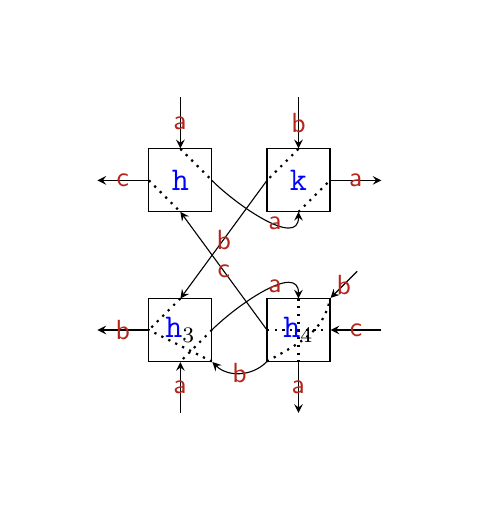
\begin{tikzpicture}[node distance=1.5cm,scale=1]
        \node (square-h) [draw,minimum width=0.8cm,minimum height=0.8cm] {\large $\HH$};
        \node [state] (h-a) [above of = square-h, draw=none] {};
        \node [state] (h-c) [left of = square-h, draw=none] {};
        \draw [-stealth] (h-a) --  node {$\msg[a]$} (square-h);
        \draw [-stealth] (square-h) --  node {$\msg[c]$} (h-c);
        \node (square-k) [draw,minimum width=0.8cm,minimum height=0.8cm, right of = square-h] {\large $\KK$};
        \node [state] (k-b) [above of = square-k, draw=none] {};
        \node [state] (k-a) [right of = square-k, draw=none] {};
        \draw [-stealth] (k-b) --  node {$\msg[b]$} (square-k);
        \draw [-stealth] (square-k) --  node {$\msg[a]$} (k-a);
        \node (square-v)  [draw,minimum width=0.8cm,minimum height=0.8cm, below of = square-h, yshift=-4mm] {\large $\hh_3$};
        \node [state] (v-b) [left of = square-v, draw=none] {};
        \node [state] (v-a) [below of = square-v, draw=none] {};
        \draw [-stealth] (v-a) --  node {$\msg[a]$} (square-v);
        \draw [-stealth] (square-v) --  node {$\msg[b]$} (v-b);
        \node (square-w)  [draw,minimum width=0.8cm,minimum height=0.8cm, below of = square-k, yshift=-4mm] {\large $\hh_4$};
        \node [state] (w-c) [right of = square-w, draw=none] {};
        \node [state] (w-a) [below of = square-w, draw=none] {};
        \node [state] (w-b) [above right of = square-w, draw=none] {};
        \draw [-stealth] (w-c) --  node {$\msg[c]$} (square-w);
        \draw [-stealth] (square-w) --  node {$\msg[a]$} (w-a);
        \draw [stealth-] (square-w) --  node {$\msg[b]$} (w-b);
        %
        \draw [-stealth] (square-w) to[out=-135,in=-45]  node {$\msg[b]$} (square-v);
        %
        \draw (0,0.4)[dotted,thick]  --  (0.4,0); % carrying a inside h  
        \draw (-0.4,0)[dotted,thick]  --  (0,-0.4); % carrying c inside h
        %
        \draw (1.5,0.4)[dotted,thick]  --  (1.1,0); % carrying b inside k
        \draw (1.5,-0.4)[dotted,thick]  --  (1.9,0); % carrying a inside k
        %
        \draw (0.4,-1.9)[dotted,thick]  --  (0,-2.3); % carrying a inside v
        \draw (0,-1.5)[dotted,thick]  --  (-0.4,-1.9); % carrying k's b inside v
        \draw (0.4,-2.3)[dotted,thick]  --  (-0.4,-1.9); % carrying b inside v
        %
        \draw (1.5,-1.5)[dotted,thick]  --  (1.5,-2.3); % carrying a inside w
        \draw (1.1,-1.9)[dotted,thick]  --  (1.9,-1.9); % carrying c inside w
        \draw (1.1,-2.3)[dotted,thick]  to[out=30,in=260]  (1.9,-1.5); % carrying b inside w
        %
        %
        \draw [-stealth]  (0.4,-1.9) to[out=45,in=90]  node [pos=0.6] {$\msg[a]$} (1.5,-1.5 ); % carryng a from v to w    
         \draw [stealth-]  (0,-0.4)  --  node  {$\msg[c]$} (1.1,-1.9); % carryng c from w to h 
        \draw [-stealth]  (0.4,0)  to[out=-45,in=-90]  node [pos=0.6]  {$\msg[a]$} (1.5,-0.4 ); % carrying a from h to k
        \draw [stealth-]  (0,-1.5)  -- node  {$\msg[b]$}  (1.1,0); % carrying  b from k to v
 \end{tikzpicture}\\[-4mm]
 \text{\small (Using $\cm_\mathrm{A}$)}
 &
 \text{\small (Using $\cm_\mathrm{B}$)}
 \end{array}$
  }
  \vspace{-1mm}
  \caption{Static description of two PaI multicompositions via gateways}
  \label{fig:multiconnection}
 \end{figure}
 Similarly to the binary case, the PaI multicomposition of the four
 systems consists in fact in replacing the participants  $\hh_1$, $\hh_2$, $\hh_3$ and $\hh_4$, chosen  as
interfaces, by gateways whose uniform task is to forward messages.
Unlike the binary case, however, in presence of more than two systems 
the gateways are not uniquely determined.
Moreover, taking into a specific connection model is not sufficient either.
This can be illustrated by looking at message $\msg[b]$ and participant $\hh_3$.
No matter whether we consider $\cm_\mathrm{A}$ or $\cm_\mathrm{B}$, it is
not determined when the gateway for $\hh_3$ will accept $\msg[b]$ 
from $\hh_2$ and when from $\hh_4$.
For instance,  
a message $\msg[b]$ from $\hh_4$ could be accepted by $\hh_3$ only after two $\msg[b]$'s are received from $\hh_2$.
A connection model is hence not enough to consent, in general, the identification of the gateways. 
A behavioural (i.e. dynamic) description of how the messages have to be
forwarded by the gateways is needed.
We represent such descriptions in terms of CFSM systems and dub them {\em connection policies}.
A connection policy is such that any interface machine, say $\hh_1$ for $S_1$,  has a corresponding
machine $\dot\hh_1$ in the connection policy with the very same structure. Moreover, for any edge of the form 
\raisebox{2mm}
{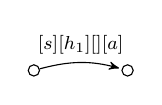
\begin{tikzpicture}[mycfsm]
      % 
      \node[state] (zero) [yshift=-4mm] {$~$};
      \node[state] (one) [right of=zero, xshift=-5mm]   {$~$};
      % 
      \path
      (zero) edge[bend left=15] node[above] {$\ain[s][h_1][][a]$} (one)
      ;
 \end{tikzpicture}
 }, i.e. a message reception of $\msg[a]$ by $\hh_1$,  
 the corresponding edge in the machine $\dot\hh_1$ has a label of the form
 \raisebox{2mm}
{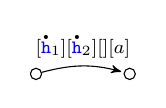
\begin{tikzpicture}[mycfsm]
      % 
      \node[state] (zero) [yshift=-4mm] {$~$};
      \node[state] (one) [right of=zero, xshift=-5mm]   {$~$};
      % 
      \path
      (zero) edge[bend left=15] node[above] {$\aout[\dot\hh_1][\dot\hh_2][][a]$} (one)
      ;
 \end{tikzpicture}
 }. The label specifies that in the composition the gateway $\hh_1$, upon reception of that particular occurence of 
 $\msg[a]$, has to forward it to the gateway $\hh_2$.
A gateway is hence built out of an interface machine and its dotted counterpart in the
communication policy used for the composition. 
 \vspace{-1mm} In particular, out of the edges 
\raisebox{2mm}
{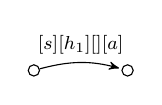
\begin{tikzpicture}[mycfsm]
      % 
      \node[state] (zero) [yshift=-4mm] {$~$};
      \node[state] (one) [right of=zero, xshift=-5mm]   {$~$};
      % 
      \path
      (zero) edge[bend left=15] node[above] {$\ain[s][h_1][][a]$} (one)
      ;
 \end{tikzpicture}
 } 
 in $\hh_1$ and 
 \raisebox{2mm}
{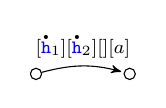
\begin{tikzpicture}[mycfsm]
      % 
      \node[state] (zero) [yshift=-4mm] {$~$};
      \node[state] (one) [right of=zero, xshift=-5mm]   {$~$};
      % 
      \path
      (zero) edge[bend left=15] node[above] {$\aout[\dot\hh_1][\dot\hh_2][][a]$} (one)
      ;
 \end{tikzpicture}
 }  
  in $\dot\hh_1$, we have
  \raisebox{2mm}
{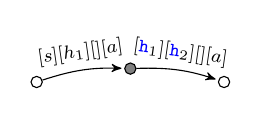
\begin{tikzpicture}[mycfsm]
      % 
      \node[state] (zero) [yshift=-4mm] {$~$};
      \node[state] (one) [right of=zero, xshift=-5mm, yshift=2mm, fill=gray]   {$~$};
       \node[state] (two) [right of=one, xshift=-5mm, yshift=-2mm,]   {$~$};
      % 
      \path
      (zero) edge[bend left=10] node[above] {$\ain[s][h_1][][a]$} (one)
      (one) edge[bend left=10] node[above] {$\aout[\hh_1][\hh_2][][a]$} (two)
      ;
 \end{tikzpicture}
 }
in the resulting gateway, where the white nodes are as in the interface  and the gray node is introduced by the gateway construction.
Recall that, in order to enforce conservativity, gateways are given the same names as the
corresponding interfaces.
The above discussion applies, dually, for edges in the interface $\hh_1$ labelled with output actions.

It is of course possible to compose, two by two, several systems using binary composition,
but in that way -- by looking at systems as vertices and gateway connections as undirected edges  -- we can get only tree-like structures of systems. By means of multicomposition
(where a single interface is considered for each system) we can get, instead, graph-like structures. 

Safety of PaI multicomposition for synchronous  MPST has been exploited in~\cite{BDGY23} 
and further investigated in~\cite{BDL22,BBD25}, where a restricted  notion of multiple connections in a client-server setting has been considered.

% the recipients of forwarded messages are not uniquely determined. 


%It is important to see that even if the CFSMs for the participants
%in the single systems were given, the connection models and the drawings 
%in~\cref{fig:multiconnection}
%do not always determine (unlike the binary case) a connection policy modelling the dynamic forwarding strategy. 




%===
%
%
%Unlike the binary case, however, in presence of more than two systems 
% the recipients of forwarded messages are not uniquely determined. 
%For instance, a message $\msg[a]$ sent to $\hh_1$ in $S_1$, could be forwarded 
%to either one of the other systems. 
%More precisely, a \emph{connection policy} has to be set up
%in order to  appropriately define the gateways. Such a policy primarily depends on
%which partner is chosen for the current message to be exchanged.
%
%
%===

\paragraph{The PaI Approach to Orchestrated Multicomposition}
Orchestration in the multicomposition setting is a natural extension of the idea
previously discussed for the binary case.  
In the present example, 
%let us consider again the four interface participants of \cref{fig:four-ips} belonging
%to the systems $S_1$,  $S_2$, $S_3$ and $S_4$. 
let us assume that we wish to get a composition such that 
$(a)$ 
any occurrence of message $\msg[a]$
received by the gateway for $\hh_1$ be forwarded not only to
the gateway for $\hh_4$ ($\cm_\mathrm{A}$) or $\hh_2$ ($\cm_\mathrm{B}$) but to both (in some sequential order);
$(b)$ 
any message $\msg[a]$ handled by $\hh_3$ be not forwarded to anyone.
This cannot be described by the connection policy which, in our intention, aims at
formalising just a forwarding strategy in a uniform way. 



%This cannot be captured by the uniform realisation of gateways which,
%upon reception of a message, must decide to which target the message should be sent.   
The  requirements $(a)$  and $(b)$  cannot be captured by the uniform forwarding strategy of gateways since
we expect the machine $\dot\hh_3$ to have the same structure of the interface machine $\hh_1$.
A realisation of our requirements would be possible only
by considering an extended notion of gateway where
the forwarding task were combined with the task of implementing the orchestrating requirements,
We wish, however, to have the forwarding task separated from the orchestrating one, i.e. to enforce Separation of Concerns (SoC), a fundamental principle in software engineering.
So, in order to obtain a composition respecting such principle and satisfying at the same time our assumed desiderata $(a)$ and $(b)$, we introduce two {\em orchestrating participants}, say $\ttd$ and $\tte$.
 The former can duplicate and forward any received message $\msg[a]$ to two distinct participants, 
whereas the latter just discards any received message $\msg[a]$.
Such a composition scenario can be described by an {\em orchestrated connection model},
graphically represented by the left diagram in~\cref{fig:orchint}.
 The  architecture of the resulting composed system 
 is represented  by the right diagram in~\cref{fig:orchint}.
 
 
 
%\brc Old text:
%We assume %also
%that in our composition we need to have the gateways for 
%$\hh_2$ and $\hh_4$ to both receive each time the very same messages $\msg[a]$ that the gateway for $\hh$ does
%forward. Moreover, we wish any message $\msg[a]$ dealt with by $\hh_3$ not to be forwarded to anyone.
%It is obviously possible to transform the implemented structure of the gateway 
%in such a way such objective are achieved. This can be done at the cost, however, of unifying the
%task of composition via forwarding gateways with the task of orchestrating the interactions among gateways.
%Mantaining instead such tasks separated would
%enforce conservativity as well as Separation of Concerns (SoC), a fundamental principle in software engineering and design.
%
%We could obtain a composition respecting such principles and satisfying at the same time our desiderata in the example by introducing two {\em orchestrating participants}, say $\ttb$ and $\ttd$.
%\brc I would use ``e`` instead of $\ttb$ since b is also the name of a message\erc 
%The former being able just to receive $\msg[a]$ messages, and the  latter able to forward twice
%any $\msg[a]$ message received. 
%Such a composition scenario can \brr be \err formalised 
% by introducing the notion of {\em (orchestrated) connection model}
% \brc I would remove the parantheses aroung ``orchestrated``\erc, graphically represented by the left diagram in~\cref{fig:orchint}.
% The  architecture of the resulting composed system obtained by means of a composition system complying with the represented orchestrated connection model, is instead represented  by the right diagram in~\cref{fig:orchint}.
% \erc end old text


\begin{figure}[h]%{c}{0.6\textwidth}
    \centering{
    \vspace{-8mm}
    $\begin{array}{c@{\qquad\qquad\qquad\qquad}c}
   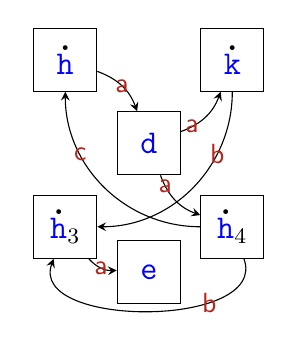
\begin{tikzpicture}[node distance=1.5cm,scale=1]
        \node (square-d) [draw,minimum width=0.8cm,minimum height=0.8cm] {\large $\ttd$};
        \node (square-h) [draw,minimum width=0.8cm,minimum height=0.8cm, above left of = square-d] {\large $\dot\HH$};
        \node (square-k) [draw,minimum width=0.8cm,minimum height=0.8cm,above right  of = square-d] {{\large $\dot\KK$}};
        \node (square-v)  [draw,minimum width=0.8cm,minimum height=0.8cm,below  left of = square-d] {{\large $\dot\hh_3$}};
        \node (square-w)  [draw,minimum width=0.8cm,minimum height=0.8cm,below  right of = square-d] {{\large $\dot\hh_4$}};
        \node (square-b) [draw,minimum width=0.8cm,minimum height=0.8cm, below of = square-d, yshift=-4pt] {\large $\tte$};
        %
        \path   (square-h) [-stealth, bend left = 25]   edge node {$\msg[a]$} (square-d)
                   (square-w) [-stealth, bend left = 45, pos=0.7]   edge node {$\msg[c]$} (square-h)
                   (square-k) [-stealth, bend left = 45, pos=0.3]   edge node {$\msg[b]$} (square-v)
                   (square-v) [-stealth, bend right = 25, pos=0.5]   edge node {$\msg[a]$} (square-b)
                   (square-w) [-stealth, bend left = 110, pos=0.3]   edge node {$\msg[b]$} (square-v)
                   (square-d) [-stealth, bend right = 25, pos=0.2]   edge node {$\msg[a]$} (square-k)
                   (square-d) [-stealth, bend right = 25, pos=0.2]   edge node {$\msg[a]$} (square-w);
 \end{tikzpicture}
    &
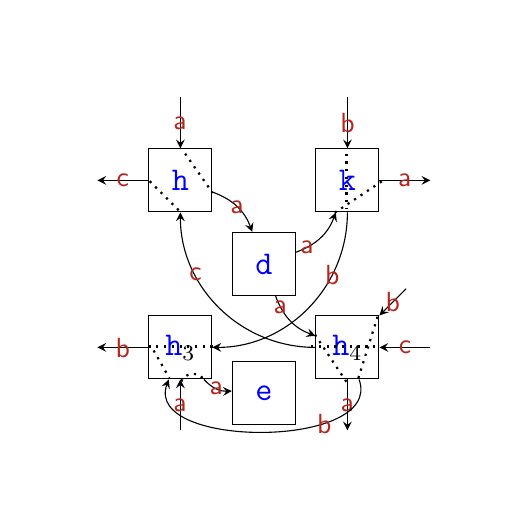
\begin{tikzpicture}[node distance=1.5cm,scale=1]
        \node (square-d) [draw,minimum width=0.8cm,minimum height=0.8cm] {\large $\ttd$};
        \node (square-b) [draw,minimum width=0.8cm,minimum height=0.8cm, below of = square-d, yshift=-4pt] {\large $\tte$};
        \node (square-h) [draw,minimum width=0.8cm,minimum height=0.8cm, above left of = square-d] {\large $\HH$};
        \node [state] (h-a) [above of = square-h, draw=none] {};
        \node [state] (h-c) [left of = square-h, draw=none] {};
        \draw [-stealth] (h-a) --  node {$\msg[a]$} (square-h);
        \draw [-stealth] (square-h) --  node {$\msg[c]$} (h-c);
        \node (square-k) [draw,minimum width=0.8cm,minimum height=0.8cm, above right of = square-d] {\large $\KK$};
        \node [state] (k-b) [above of = square-k, draw=none] {};
        \node [state] (k-a) [right of = square-k, draw=none] {};
        \draw [-stealth] (k-b) --  node {$\msg[b]$} (square-k);
        \draw [-stealth] (square-k) --  node {$\msg[a]$} (k-a);
        \node (square-v)  [draw,minimum width=0.8cm,minimum height=0.8cm, below left of = square-d] {\large $\hh_3$};
        \node [state] (v-b) [left of = square-v, draw=none] {};
        \node [state] (v-a) [below of = square-v, draw=none] {};
        \draw [-stealth] (v-a) --  node {$\msg[a]$} (square-v);
        \draw [-stealth] (square-v) --  node {$\msg[b]$} (v-b);
        \node (square-w)  [draw,minimum width=0.8cm,minimum height=0.8cm, below right of = square-d] {\large $\hh_4$};
        \node [state] (w-c) [right of = square-w, draw=none] {};
        \node [state] (w-a) [below of = square-w, draw=none] {};
        \node [state] (w-b) [above right of = square-w, draw=none] {};
        \draw [-stealth] (w-c) --  node {$\msg[c]$} (square-w);
        \draw [-stealth] (square-w) --  node {$\msg[a]$} (w-a);
        \draw [stealth-] (square-w) --  node {$\msg[b]$} (w-b);
        %
        \draw (-1,1.4)[dotted,thick]  --  (-0.65,0.9); % carrying a inside h  
        \draw (-1.45,1.05)[dotted,thick]  --  (-1.05,0.65); % carrying c inside h
        %
        \draw (1.05,1.4)[dotted,thick]  --  (1.05,0.7); % carrying b inside k
        \draw (0.9,0.65)[dotted,thick]  --  (1.5,1.05); % carrying a inside k
        %
        \draw (-0.65,-1.05)[dotted,thick]  --  (-1.5,-1.05); % carrying b inside v
        %%\draw (0,-1.5)[dotted,thick]  --  (-0.4,-1.9); % carrying k's a inside v
        \draw (-1.4,-1.1)[dotted,thick]  --  (-1.2,-1.45); % carrying b inside v
        %
        \draw (.65,-0.9)[dotted,thick]  --  (1.05,-1.5); % carrying a inside w
        \draw (0.6,-1.05)[dotted,thick]  --  (1.45,-1.05); % carrying c inside w
        \draw (1.2,-1.45)[dotted,thick] --  (1.45,-0.65); % carrying b inside w
        %
        %
        \path   (square-h) [-stealth, bend left = 25]   edge node {$\msg[a]$} (square-d)
                   (square-w) [-stealth, bend left = 45, pos=0.7]   edge node {$\msg[c]$} (square-h)
                   (square-k) [-stealth, bend left = 45, pos=0.3]   edge node {$\msg[b]$} (square-v)
                   (square-v) [-stealth, bend right = 25, pos=0.5]   edge node {$\msg[a]$} (square-b)
                   (square-w) [-stealth, bend left = 110, pos=0.3]   edge node {$\msg[b]$} (square-v)
                   (square-d) [-stealth, bend right = 25, pos=0.2]   edge node {$\msg[a]$} (square-k)
                   (square-d) [-stealth, bend right = 25, pos=0.2]   edge node {$\msg[a]$} (square-w);
         \draw  (-0.78,-1.45)[dotted,thick]  to[out=120,in=80]  (-1.05,-1.5); % carrying a inside v
 \end{tikzpicture}
 \end{array}$
 \vspace{-6mm}
 }
 \caption{\label{fig:orchint} An orchestrated connection model (left)  and the resulting orchestrated composition (right).}
 \end{figure}

\noindent
The \emph{orchestrated multicomposition} of $n$ systems of CFSMs -- according to
a chosen set of interfaces and a connection policy -- 
is then simply obtained by $(1)$ taking all the machines of the single systems;
$(2)$ replacing each interface machine by the gateway built out of the interface and its 
dotted counterpart in the connection policy; $(3)$ adding the 
orchestrating participants possibly contained in the orchestrated connection policy.

\medskip

It is worth noticing that orchestrated composition
can be looked at as an unorchestrated multicomposition where one system is allowed to have multiple
interfaces. 

A system obtained by orchestrated composition can be actually viewed as a tree of systems
with  the orchestrated policy as root. 
It is hence fairly natural to wonder whether an orchestrated composition can be simply obtained
by a number of binary compositions between the orchestrated connection policy and 
the systems we wish to compose. 
This is however not the case. We recall, in fact, that in an orchestrated connection policy 
the participants with dotted names (like $\dot\hh_1,\dot\hh_2,\dot\hh_3$ and $\dot\hh_4$ above) are not (and are not treated as) actual interfaces. They describe the forwarding policy to be implemented in the contruction of the gateways from the (undotted) interfaces in the systems.



  It is worth remarking that, by introducing suitable orchestrating participants, we could also  compose
systems dealing with different sets of messages.
 For example, an orchestrating participant could rename a received message before forwarding it.
Such a feature would turn out to be quite relevant in practice whenever the systems we compose
use different names to represent the very same information. 
We could also think about a gateway forwarding an information needing to be somewhat processed
before the other gateway receives it.




  

%\brc
%I would remove the next two sentences.\erc
%It would be possible to centralise all the orchestrating task into a single orchestrating participant.
%Such a possibility is entailed by our approach but, even if it would make the generation of the gateways completely uniform, might severely prevent the gateway to be loosely coupled.
%
%\brc
%I have moved the next sentence up.\erc.
%It is worth remarking that, by introducing suitable orchestrating participants, we could also  compose
%systems using interfaces that do not deal with the same message names.

\noindent
\paragraph{Contributions}
%\brc
%I wonder whether parts of the following literature have been included already earlier (end of page 5,
%top of page 7). But we can also keep it as it is.
%\erc
 In the present paper we investigate safety of PaI multicomposition for the asynchronous formalism of CFSMs generalising  our recent work 
 \cite{BH24} by taking into account {\em orchestrated} multicomposition.
The idea of PaI multicomposition was introduced in~\cite{BDGY23} for a synchronous MPST framework
and without orchestration. 
With respect to synchronous MPST, the present asynchronous CFSM setting needs completely different design and proof techniques, in
particular in the presence of orchestrating participants. 
We go beyond both the PaI binary composition of asynchronous CFSMs of~\cite{BdLH19}
and the PaI multicomposition of~\cite{BH24}, where the interactions among the gateways were 
driven by connection policies (see \cref{sec:pai-multicomp} below) without orchestration.
Clearly this goes also beyond the aforementioned papers~\cite{BLT20,BLP22b,BLT23} dealing with binary composition of synchronous CFSMs. In particular, in the asynchronous case different communication properties, like unspecified-reception freedom or orphan-message freedom, are relevant. 

A crucial role in our approach to orchestrated multicomposition is played by
{\em connection policies} which are themselves systems of CFSMs mediating between the systems to be composed. They can be individually chosen 
by the system designer on the basis of a given concrete  \emph{connection model}.
%A connection model describes architectural aspects of compositions.
%It specifies which forwarding links among interface participants of different systems 
%-- as well as possible orchestrating participants --
%are meaningful from a static perspective.
In multicomposition, gateways are determined by the orchestrated connection policy 
which therefore also determines the channels used by the gateway CFSMs.
The ``structure'' of the gateways (i.e. when we look at them disregarding the channels they use)
is instead uniformly and uniquely determined,
so mantaining the intrinsic conservativity of the PaI approach also in the present case.

The use of connection models  is methodologically important 
since it is more likely that an orchestrated connection policy complying with a connection model will satisfy desired communication properties.
For the proofs of our safety results, however, only the specifics of the chosen orchestrated connection policy are relevant.

We show that a number of relevant communication properties
(deadlock-freedom, orphan-message freedom, unspecified-reception freedom, and progress) are preserved by PaI orchestrated multicomposition of CFSM systems
whenever the particular property is satisfied also by the orchestrated connection policy used. 
Apart from orphan-message-freedom preservation we need, however, an additional assumption which requires that interface participants do not
have a state with at least one outgoing output action and one
outgoing input action, 
a condition referred to in the literature as {\em no-mixed-state}~\cite{CF05}.
It is worth remarking that for each property, safety is proven on the condition the same property 
holds for the connection policy, i.e. we do not require a general property 
(like {\em compatibility} in the binary case) entailing all the communication properties.  
 We provide counterexamples illustrating the role played by the no-mixed-state condition
in guaranteeing safety of composition.
 In contrast to deadlock-freedom, the stronger property of lock-freedom
will be shown (by means of a counterexample) not to be preserved in general, even in the absence of mixed-states. 


\paragraph{Outline of the paper}
 The main ideas underlying PaI orchestrated multicomposition  have been   
 intuitively described  above in \cref{sec:pai-multicomp}.
%  It will be preceded by an introduction to PaI multicomposition (i.e. non-orchestrated).
In \cref{sect:cfsm} we recall  the definitions of communicating finite state machine, communicating system and their related notions.  
There we also provide the definitions of a number of relevant communication properties. 
In \cref{sec:opensys}, PaI orchestrated multicomposition is formally defined  on the basis  of the definitions of orchestrated connection policy and gateway. 
Our main  results  are presented in~\cref{sec:preservation}
including counterexamples spotting the role of the no-mixed-state condition and a counterexample
for lock-freedom preservation. 
In \cref{sect:safetypreservation} the key notion of projection used in proofs and some technical lemmas are presented. The proofs of the single preservation results are provided in \cref{sect:presres}.
\cref{sect:related-work} reviews some alternative approaches to system composition
highlighting the similarities with our approach, if any. 
\cref{sect:conclusions} concludes with a brief summary and a few hints for future work. 


\paragraph{Comparison with the workshop version}
In the workshop paper~\cite{BH24} we have presented multicomposition of systems of asynchronously
communicating finite state machines extending ideas of binary asynchronous composition in ~\cite{BdLH19}.
%A central notion in~\cite{BH24} was the concept of connection policy which is itself a system of CFSMs.
%Our crucial result showed that relevant communication properties, like freedom of unspecified reception
%and orphan messages, are preserved by system composition if the connection policy at hand satisfies these properties. 
It turned out, however, that connection policies which can be realised just by introducing gateways is not powerful enough in practice; see the discussion in~\cref{sec:pai-multicomp}
and our extended -- with respect to ~\cite{BH24} -- running example.
The current paper goes beyond~\cite{BH24}, allowing to orchestrate connection policies with the help of so-called orchestrating participants. This leads to our notion of \emph{orchestrated connection policy}. We generalise the concepts of connection model and multicomposition of CFSM systems by allowing orchestrated connection policies and we show that preservation of communication properties is also ensured once an orchestrated connection policy - used for system composition -
enjoys the relevant communication properties. An essential part of the present paper is devoted to proofs
of our preservation results. These proofs subsume as special cases also the results of the workshop paper, which could only give a few hints for the proofs. 
The extension of the proofs from ~\cite{BH24} to the present orchestration case is not straighforward since we have to show that, roughly, the projection of
a reachable configuration on a communication policy is reachable also in presence of orchestrating 
participants.  











%!TEX root = Main-CFSM-partial-fusion.tex
\section{Systems of Communicating Finite State Machines}
\label{sect:cfsm}

Communicating Finite State Machines (CFSM)   are 
 a widely investigated
formalism for the description and analysis of distributed systems, originally proposed in \cite{BZ83}.
CFSM are a variant of finite state I/O-automata that represent processes which communicate by asynchronous exchanges of messages via FIFO channels. 
We now recall (partly following \cite{CF05,DY12,TY15,BdLH19}) the definitions of CFSM and systems of CFSMs.

We assume %given 
a countably infinite set  
$\roles_\mathfrak{U}$ of participant names (ranged over by $\ttp,\ttq,\ttr,\HH,\KK,\ttv,\ttw\ldots$) and a countably infinite alphabet $\mathbb{A}_\mathfrak{U}$ 
of messages (ranged over by $\msg[a]$, $\msg[b]$, $\msg[c]$, $\msg[m],\ldots$).\\

\begin{definition}[FSA and $\varepsilon$-FSA with no final states]
 
\end{definition}
** Explain that we start from the very general definition of FSA since we shall use results on FSA like
the elimination of $\varepsilon$-transitions-

\begin{definition}[CFSM**TO BE DEFINED SIMPLY AS FSA on $\textit{Act}_{\roles,\mathbb{A}}$ with NO FINAL STATES**]\label{def:cfsm}%\hfill\\
Let $\roles$  and $\mathbb{A}$ be finite subsets of $\roles_\mathfrak{U}$ and $\mathbb{A}_\mathfrak{U}$, respectively.
\begin{enumerate}[i)] 
\item
The set $C_\roles$ of {\em channels} over $\roles$ is defined by\ \
$C_\roles=\Set{\ttp\ttq \mid \ttp,\ttq\in \roles, \ttp\neq\ttq}$
\item
The set $\mathit{Act}_{\roles,\mathbb{A}}$ of {\em actions}  over $\roles$ and $\mathbb{A}$ is defined by\ 
$\textit{Act}_{\roles,\mathbb{A}} = C_\roles\times\Set{!,?}\times\mathbb{A}$

The {\em subject} of an output action $\ttp\ttq!\msg[m]$ and of an input action $\ttq\ttp?\msg[m]$ is 
$\ttp$.
\item
\label{def:cfsm-iii}
A {\em communicating finite state machine over} $\roles$ \emph{and} $\mathbb{A}$
is a finite transition system given by a tuple\\
\centerline{ $M=(Q,q_0,\mathbb{A},\delta)$ }
where $Q$ is a finite set of states, $q_0\in Q$ is the initial state, and
$\delta\subseteq Q\times\textit{Act}_{\roles,\mathbb{A}}\times Q$ is a set of transitions
such that all the actions have the same subject, to which we refer as the {\em name} of $M$.
\end{enumerate}
\end{definition}
\noindent
We shall write $M_{\ttp}$ to denote a CFSM with name $\ttp$. 
Where no ambiguity arises we shall refer to a CFSM by its name.


Notice that the above definition of CFSM is generic with respect to the underlying sets
$\roles$ and $\mathbb{A}$.
This is necessary,  since we shall not deal with a single system of CFSMs but with an arbitrary number of  systems of CFSMs that can be {\em composed}.
We shall write $C$ and $\mathit{Act}$ instead of $C_\roles$ and $\mathit{Act}_{\roles,\mathbb{A}}$ when no ambiguity can arise.
%\brc Let us check whether we ever use $C$ and $\mathit{Act}$.
%But even then, I would prefer to see $C_\roles$ and $\mathit{Act}_{\roles,\mathbb{A}}$ which is minimal longer.\erc
 We assume $\elle,\elle',\ldots$ to range over $\textit{Act}$
%$\varphi,\varphi',\ldots$ to range over $\textit{Act}^*$ (the set of finite words over $\textit{Act}$), 
and $w,w',\ldots$ to range over $\mathbb{A}^*$ (the set of finite words over $\mathbb{A}$).
The symbol $\varepsilon\,(\notin \mathbb{A}\cup\textit{Act})$ denotes the empty word and 
$\mid w\mid$ the length of a word $w\in \mathbb{A}^*$.
%$\mid v\mid$ the lenght of a word $v\in \textit{Act}^*\cup\mathbb{A}^*$.

%%>>>>>>>> DEFINITIONS NOT USED in the present paper
%Given a word $v$ with prefix $v'$, i.e. such that $v=v'\cdot v''$ for a certain $v''$, we define $v\setminus v' =v''$.
%Moreover, given a  word $v$ with $\msg[a]$ as last  element, i.e. $v=v'\cdot \msg[a]$ for a certain (possibly empty) $v'$, we define
%$\mathsf{init}(v) = v'$ and  $\mathsf{last}(v) = \msg[a]$. 
%Moreover, we shall denote by $\widetilde{v}$ the reverse of the word $v$. \\


The transitions of a CFSM are labelled by actions; a label $\tts\ttr!\msg[a]$ represents
the asynchronous sending of message $\msg[a]$ from machine $\tts$ to $\ttr$ through channel $\tts\ttr$ and, dually,
$\tts\ttr?\msg[a]$ represents the reception (consumption) of $\msg[a]$ by $\ttr$ from channel
$\tts\ttr$. 

 Given a CFSM $M=(Q,q_0,\mathbb{A},\delta)$,
we also define \\
\centerline{$\inn{M}=\Set{\msg[a] \mid (\_,\_\,\_?\msg[a],\_)\in \delta }$
\quad \text{ and }\quad $\outt{M}=\Set{\msg[a] \mid (\_,\_\,\_!\msg[a],\_)\in \delta }$.}
 If $M$ is a CFSM with name $\ttp$, we also write $\inn{\ttp}$ for $\inn{M}$ and
 $\outt{\ttp}$ for $\outt{M}$.
  Note that, in concrete examples, the name of a CFSM together with its input and output messages can be graphically depicted as in~\cref{fig:four-ips}. 




%We write $\lang{M}\subseteq\textit{Act}^*$ for
%the language over $\textit{Act}$ accepted by the automaton corresponding
%to machine $M$, where each state of $M$ is an accepting state. 
A state
$q\in Q$ with no outgoing transition is {\em final}; 
$q$ is a {\em sending} (resp. {\em receiving}) state if it is not final and
all outgoing transitions are labelled with sending (resp. receiving) actions;
$q$  is a {\em mixed} state if there are at least two outgoing transitions such that one is labelled with a sending action and the other one is labelled with a receiving action.



%
%  ?!-DETERMINISM DEFINITION <<<<<<<<<<<<<<<<<<<<<<<<
% 
%\vspace{2mm}
%A CFSM $M = (Q,q_0,\mathbb{A},\delta)$ is:
%\begin{enumerate}[a)]
%\item
% {\em deterministic} if for all transitions:\quad % states $q\in Q$ and all actions $\elle$: 
%$(q,\elle, q'), (q,\elle,q'')\in \delta$ imply $q'=q''$;
%\item
%{\em ?-deterministic} (resp. {\em !-deterministic}) if for all transitions:\\ % all states  $q\in Q$ and all actions:\\
%$\qquad$ $(q,\ttr\tts?\msg[a], q'), (q,\ttp\ttq?\msg[a],q'')\in \delta$ (resp. $(q,\ttr\tts!\msg[a], q'), (q,\ttp\ttq!\msg[a],q'')\in \delta$) imply $q'=q''$;\footnote{Note that, by Definition \ref{def:cfsm}(\ref{def:cfsm-iii}), we have
%necessarily that $\tts=\ttq$ in the clause for ?-determinism and $\ttr=\ttp$ in the one for
%!-determinism.}
%\item
%{\em ?!-deterministic} if it is both ?-deterministic and !-deterministic.
%\end{enumerate}
%
%The notion of ?!-deterministic machine is more demanding than in usual CFSM settings. It will be needed in order to guarantee preservation of communication properties when systems are connected. 
%Note that a ?!-deterministic CFSM is also deterministic, but the converse does not hold
%(since the channel names are abstracted away in the definition of ?!-determinism). \\

A {\em communicating system}, called ``protocol'' in \cite{BZ83}, is a finite set of CFSMs.
% over some vocabulary of messages such that senders and receivers are identified by the 
%names of CFSMs. 
 In~\cite{CF05,DY12,TY15} the names of the CFSMs in a system are called {\em roles}. In the present paper we call them {\em participants}.
 

The dynamics of a system are
formalised as a transition relation on configurations, where a configuration is a
pair of tuples: a tuple of states of the machines in the system and a tuple of buffers representing the content of the channels. A buffer is described as an element of $\mathbb{A^*}$. 

\begin{definition}[Communicating system and configuration]%\hfill\\
Let $\roles$  and $\mathbb{A}$ be as in Def.~\ref{def:cfsm}.
\begin{enumerate}[i)]
\item
A {\em communicating system (CS)
over} $\roles$ \emph{and} $\mathbb{A}$ is a  set  %tuple 
$S= (M_\ttp)_{\ttp\in\roles}$
%\centerline{$S= (M_\ttp)_{\ttp\in\roles}$}
where\\
%\\
%-  $\roles\subseteq_{\text{fin}}\roles_\mathfrak{U}$   is the set of {\em roles} (participants) of $S$, and\\
for each $\ttp\in \roles$,
$M_\ttp=(Q_\ttp,q_{0\ttp},\mathbb{A},\delta_\ttp)$ is a CFSM  over $\roles$ and $\mathbb{A}$.
\item
A {\em configuration} of a system $S$ is a pair $s = (\vec{q},\vec{w})$
%\centerline{$s = (\vec{q},\vec{w})$}
where\\
\centerline{$\vec{q}= (q_\ttp)_{\ttp\in\roles}$ with $q_\ttp \in Q_\ttp$,
\qquad and \qquad  $\vec{w}  = (w_{\ttp\ttq})_{\ttp\ttq\in C}$ with $w_{\ttp\ttq}\in\mathbb{A^*}$.}
%\begin{itemize}
%\item[-]  $\vec{q}= (q_\ttp)_{\ttp\in\roles}$ with $q_\ttp \in Q_\ttp$,
%\item[-]  $\vec{w}  = (w_{\ttp\ttq})_{\ttp\ttq\in C}$ with $w_{\ttp\ttq}\in\mathbb{A^*}$.
%\end{itemize}

The component $\vec{q}$ is the {\em control state\/} of the system and $q_\ttp \in Q_\ttp$ is the 
{\em local state\/} of machine $M_\ttp$. 
The component $\vec{w}$ represents the state of the channels of the system and $w_{\ttp\ttq} \in \mathbb{A}^*$ is the state of the channel $\ttp\ttq$, i.e. the messages sent from $\ttp$ to $\ttq$. The initial configuration of $S$ is $s_0=  (\vec{q_0},\vec{\varepsilon})$
with $\vec{{q_0}} = (q_{0_\ttp})_{\ttp\in\roles}$.
\end{enumerate}
\end{definition}

\noindent
In the following we will often denote a communicating system $(M_{\ttp})_{\ttp\in \Set{\ttr_i}_{i\in I}}$ by $(M_{\ttr_i})_{i\in I}$.



\begin{definition}[Transitions and reachable configurations]
Let $S$ be a communicating system over $\roles$ and $\mathbb{A}$, and let $s= (\vec{q},\vec{w})$ and $s'= (\vec{q'},\vec{w'})$ 
be two configurations of $S$. %\\
Configuration $s'$ {\em is reachable from} $s$
{\em by firing  a transition} with action $\elle$, written $s\lts{\elle}s'$, if there is $\msg[a]\in\mathbb{A}$
such that one of the following conditions holds:
%\begin{center}
%\begin{tabular}{ r l r l}
%$1.$ & $\elle = \tts\ttr!\msg[a]$ and $(q_\tts,\elle,q'_\tts)\in\delta_\tts$ and &  
%$2.$ & $\elle = \tts\ttr?\msg[a]$ and $(q_\ttr,\elle,q'_\ttr)\in\delta_\ttr$ and\\
%        & $a)$ for all $\ttp\neq\tts: ~ q'_\ttp =  q_\ttp$  and &
%        & $a)$ for all $\ttp\neq\ttr: ~ q'_\ttp =  q_\ttp$  and \\
%        & $b)$ $w'_{\tts\ttr} =  w_{\tts\ttr}\cdot \msg[a]$ and for all $\ttp\ttq\neq\tts\ttr: ~ w'_{\ttp\ttq} =  w_{\ttp\ttq}$; &
%        & $b)$  $w_{\tts\ttr} =  \msg[a]\cdot w'_{\tts\ttr}$ and for all $\ttp\ttq\neq\tts\ttr: ~w'_{\ttp\ttq} =  w_{\ttp\ttq}$.
%\end{tabular}
%\end{center}
\begin{enumerate}
\item
$\elle = \tts\ttr!\msg[a]$ and $(q_\tts,\elle,q'_\tts)\in\delta_\tts$ and
\qquad \begin{enumerate}[a)]
\item
for all $\ttp\neq\tts: ~ q'_\ttp =  q_\ttp$  and
\item
$w'_{\tts\ttr} =  w_{\tts\ttr}\cdot \msg[a]$ and for all $\ttp\ttq\neq\tts\ttr: ~ w'_{\ttp\ttq} =  w_{\ttp\ttq}$;
\end{enumerate}
\item 
$\elle = \tts\ttr?\msg[a]$ and $(q_\ttr,\elle,q'_\ttr)\in\delta_\ttr$ and
\begin{enumerate}[a)]
\item
for all $\ttp\neq\ttr: ~ q'_\ttp =  q_\ttp$  and
\item
$w_{\tts\ttr} =  \msg[a]\cdot w'_{\tts\ttr}$ and for all $\ttp\ttq\neq\tts\ttr: ~w'_{\ttp\ttq} =  w_{\ttp\ttq}$.
\end{enumerate}
\end{enumerate}
We write $s\lts{}s'$ if there exists $\elle$ such that  $s\lts{\elle}s'$
 and we write $s\notlts{}\hspace{2mm}$ if no $s'$ and no $\elle$ exist with
$s\lts{\elle}s'$.
As usual, we denote the reflexive and transitive 
closure of $\lts{}$ by $\to^*$.
The set of {\em reachable configurations} of S is $\RS(S) = \Set{s \mid s_0 \to^* s}.$
\end{definition}
\noindent
According to the above definition, communication happens asynchronously via buffered channels following the FIFO principle.\\


\begin{example}{\em
As sketched in the Introduction, CFSMs can be graphically represented as in the following
simple example of a communicating system describing an asynchronous protocol of mutually exclusive use of
a resource by two participants $\msg[p]$ and $\msg[q]$ controlled  by a participant $\msg[c]$.
$$
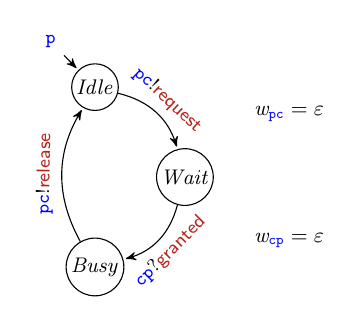
\begin{tikzpicture}[mycfsm]
  \node[state]           (idle)                        {\small $\mathit{Idle}$};
  \node[draw=none,fill=none] (wpc) [right of = idle, xshift=10mm,yshift=-4mm]{\small$\mathit{w}_{\ptp[p]\ptp[c]}=\varepsilon$};
   \node[draw=none,fill=none] (start) [above left = 0.3cm  of idle]{$\ptp[p]$};
  \node[state]           (wait) [below right of=idle] {\small $\mathit{Wait}$};
  \node[state]            (busy) [below left of=wait] {\small $\mathit{Busy}$};
    \node[draw=none,fill=none] (wcp) [right of = busy, xshift=10mm,yshift=4mm]{\small$\mathit{w}_{\ptp[c]\ptp[p]}=\varepsilon$};

   \path  (start) edge node {} (idle) 
             (idle)        edge   [bend left]      node [above]  {${\ttp\ttc}!{\msg[request]}$} (wait)
             (busy)        edge  [bend left]         node [above] {${\ttp\ttc}!{\msg[release]}$} (idle)
             (wait)  edge  [bend left]      node [below] {${\ttc\ttp}?{\msg[granted]}$} (busy);       
             \end{tikzpicture}
\qquad
\begin{tikzpicture}[mycfsm]
  \node[state]           (noreq)                        {\small $\mathit{no\text{-}reqs}$};
   \node[draw=none,fill=none] (start) [above left = 0.3cm  of idle]{$\ptp[c]$};
  \node[state]           (qreq) [below right of=idle,xshift=8mm] {\small $\mathit{\mathtt{q}\text{-}req}$};
  \node[state]           (preq) [below left of=idle,xshift=-8mm] {\small $\mathit{\mathtt{p}\text{-}req}$};
  \node[state]            (qgrant) [below left of=wait,xshift=8mm,yshift=-4mm] {\small $\mathit{\mathit{\mathtt{q}\text{-}grant}}$};
  \node[state]            (pgrant) [below left of=wait,xshift=-8mm,yshift=-4mm] {\small $\mathit{\mathit{\mathtt{p}\text{-}grant}}$};
%
   \path  (start) edge node {} (noreq) 
             (noreq)        edge   [bend left]      node [above]  {${\ttq\ttc}?{\msg[request]}$} (qreq)
             (qgrant)        edge          node [above] {${\ttq\ttc}?{\msg[release]}$} (noreq)
             (qreq)  edge  [bend left]      node [below] {${\ttc\ttq}!{\msg[granted]}$} (qgrant)
             (noreq)        edge   [bend right]      node [above]  {${\ttp\ttc}?{\msg[request]}$} (preq)
             (pgrant)        edge          node [above] {${\ttp\ttc}?{\msg[release]}$} (noreq)
             (preq)  edge  [bend right]      node [below] {${\ttc\ttp}!{\msg[granted]}$} (pgrant);       
             \end{tikzpicture}
\qquad
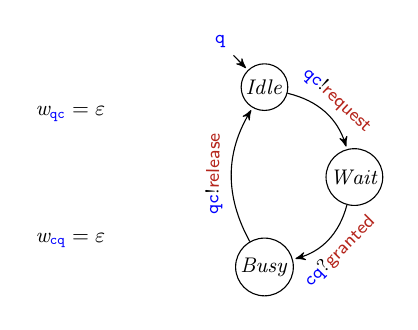
\begin{tikzpicture}[mycfsm]
  \node[state]           (idle)                        {\small $\mathit{Idle}$};
  \node[draw=none,fill=none] (wpc) [left of = idle, xshift=-10mm,yshift=-4mm]{\small$\mathit{w}_{\ptp[q]\ptp[c]}=\varepsilon$};
   \node[draw=none,fill=none] (start) [above left = 0.3cm  of idle]{$\ptp[q]$};
  \node[state]           (wait) [below right of=idle] {\small $\mathit{Wait}$};
  \node[state]            (busy) [below left of=wait] {\small $\mathit{Busy}$};
    \node[draw=none,fill=none] (wcp) [left of = busy, xshift=-10mm,yshift=4mm]{\small$\mathit{w}_{\ptp[c]\ptp[q]}=\varepsilon$};

   \path  (start) edge node {} (idle) 
             (idle)        edge   [bend left]      node [above]  {${\ttq\ttc}!{\msg[request]}$} (wait)
             (busy)        edge  [bend left]         node [above] {${\ttq\ttc}!{\msg[release]}$} (idle)
             (wait)  edge  [bend left]      node [below] {${\ttc\ttq}?{\msg[granted]}$} (busy);       
             \end{tikzpicture}
 $$
 The following configuration
 $$
 ((\mathit{Idle}_{\ttp},\mathit{\mathtt{q}\text{-}grant}_{\ttc},\mathit{Wait}_{\ttq}),
  (\mathit{w}_{\ptp[p]\ptp[c]}=\langle\msg[release]\rangle,
   \mathit{w}_{\ptp[c]\ptp[p]}=\varepsilon,
   \mathit{w}_{\ptp[q]\ptp[c]}=\langle\msg[request]\rangle,
    \mathit{w}_{\ptp[c]\ptp[q]}=\varepsilon)
)
$$
is reachable from the initial configuration after that both $\ptp[p]$ and $\ptp[q]$ have requested the resource,
$\ptp[c]$ has granted it to $\ptp[p]$ and, after acquiring it, $\ptp[p]$ has sent to $\ptp[c]$ the information
about its release. In the rest of the paper we do not show channels in drawings 
%draw the channel 
when their representation is not strictly necessary.
\finex
}\end{example}


%DEFINITIONS NOT USED in the present paper 
%%>>>>>>>>>>>
%We shall use $\xi, \xi', \ldots$ to range over sequences of transitions of the form 
%$s_1\lts{\elle_2}s_2\lts{\elle_3} \ldots \lts{\elle_{n-1}}s_{n-1}\lts{\elle_{n}}s_{n}$.
%If $\xi = s_1\lts{\elle_2} \ldots \lts{\elle_{n}}s_{n}$ we denote by $|\xi|$ its length, defined as $|\xi| = n-1$.
%In case $n=1$ we have a degenerate transition sequence of lenght $0$ made of a single configuration.\\
%We shall denote by
%$\upto{\xi}{i}$ the subsequence of the first $i$ transitions of a sequence $\xi$.\\
%Let $\xi$ be a sequence of the form $s_1\lts{\elle_2} \ldots \lts{\elle_{n-1}}s_{n-1}$, and let $s_{n-1}\lts{\elle_n}s_n$.
%We shall denote by $\xi\lts{\elle_n}s_n$  the transition sequence
%$s_1\lts{\elle_2} \ldots \lts{\elle_{n-1}}s_{n-1}\lts{\elle_n}s_n$.





%%%%%%%%%%%%%%%%%%%%%
%\textbf{Rolf: I have changed reference \cite{BZ83} in the title of the next definition to  \cite{DY12} because the latter uses exactly the definition that you give in i) below
%and which is different from our submitted paper.\\
%I have adjusted the proofs later to the new deadlock definition which is,
%if there are final states, in general not equivalent to the old one given in the submission.\\
%\cite{DY12}
%and~\cite{CF05} use the same definition of deadlock as in i) below. 
%The definition in~\cite{TY15} is different (it is the one used in our submitted version). Also the definition in~\cite{TG18} is different, see page 23 in~\cite{TG18}.
%There they say ``This defintion is adpated from~\cite{CF05}.''  
%By ``adapted'' they mean obviously that the definition has been slightly changed.
%The deadlock definition in~\cite{BZ83} is still different, because there a deadlock would already occur if all CFSMs are in a final state. This would also be a deadlock 
%in~\cite{TG18} if not all buffers are empty. 
%\\
%In summay:\\
%Deadlock in~\cite{CF05} = deadlock in~\cite{DY12} = deadlock above in i).\\
%Deadlock in~\cite{DY12} implies deadlock in~\cite{TY15} implies deadlock in~\cite{TG18} implies deadlock in~\cite{BZ83}.} \\
%%%%%%%%%%%%%%%%%%%%%%%






%\begin{definition}[Interfacing Policy]\label{def:intpol}
%An {\em interfacing policy} $\inp$ for a multiparty session $\Pi_{i\in I}{\pP{\hh_i}{\PH_i}}$ is a multiparty session $\Pi_{i\in I}{\pP{\hh_i}{\PK_i}}$ such that
%$\PK_i\in\GS{\PH_i}{\SP\setminus\set{\hh_i}}$ for all $i\in I$,  where $\SP=\set{\hh_i\mid i\in I}$.
%% $\SP=\set{\hh_i\mid i\in I}$ and $\PK_i\in\GS{\PH_i}{\SP\setminus\set{\hh_i}}$ for all $i\in I$.
%An interfacing policy is {\em valid} if $\inp$ is typable.
%\end{definition}

%\begin{example}[Interfacing policies]\label{simplewe3}
% Let us consider the four sessions of Example~\ref{simplewe4}. 
%Then an interfacing policy for the multiparty session $\Pi_{i=1}^{4}\pP{\hh_i}{\PH_i}$ is the multiparty session $\Pi_{i=1}^{4}\pP{\hh_i}{\PK_i}$
% where
% \Cline{
% \PK_1=
%\hh_3 ?\msg{start}.\,\hh_4!\msg{react}.\hh_2 !
%\left\{ \begin{array}{l}                                                                                                                                           \msg{rc}.\,\hh_2 ?\msg{img}.\,\PK_1                                                                                                                                \\
%\msg{nc}.\,\hh_2 ?\msg{img}.\,\PK_1                                                                          \end{array}\right.
%}
% \Cline{\PK_2=
%\hh_3 !\msg{react}.\,\hh_4 ?\msg{pars}.\,\hh_1 ?
%\left\{ \begin{array}{l}                                                                                                                                           \msg{rc}.\,\hh_1!\msg{img}.\,\PK_2                                                                                                                                \\
%\msg{nc}.\,\hh_1!\msg{img}.\,\PK_2
%       \end{array}\right.
%}
% \Cline{\PK_3=
%\hh_1 !\msg{start}.\,\hh_2 ?\msg{react}.\,\PK_3
%\qquad
% \PK_4=
%\hh_1 ?\msg{react}.\,\hh_2 ! \msg{pars}.\,\PK_4
%}
%
%\noindent
% This policy is valid, since the multiparty session $\Pi_{i=1}^{4}\pP{\hh_i}{\PK_i}$ can be typed by the following global type
% \Cline{
% \G=
%\hh_3\to\hh_1{:}\msg{start}.\,\hh_2\to\hh_3{:}\msg{react}.\,\hh_1\to\hh_4{:}\msg{react}.\, \hat\G}
%where
%\Cline{ \hat\G=\hh_4\to\hh_2{:}\msg{pars}.\,
%\hh_1\to\hh_2{:}
%\left\{ \begin{array}{l}                                                                                                                                           \msg{rc}.\,\hh_2\to\hh_1{:}\msg{img}.\,\G \\
%\msg{nc}.\,\hh_2\to\hh_1{:}\msg{img}.\,\G                                                                          \end{array}\right.}
%Note that, according to the above interfacing policy, the greeting depends on the reactions sent by the sensor driven by $\pq$.
% It is not difficult to check that there exists another valid interfacing policy for $\Pi_{i=1}^4{\pP{\hh_i}{\PH_i}}$, namely the one according to which the greeting depends on the reactions sent by the sensor driven by $\pp$.  I.e.  also  $\Pi_{i=1}^{4}\pP{\hh_i}{\PK_i'}$  is  an interfacing policy for the multiparty session $\Pi_{i=1}^{4}\pP{\hh_i}{\PH_i}$ 
% where
% \Cline{
% \PK'_1=
%\hh_3 ?\msg{start}.\,  \hh_3 !\msg{react}.\,  %\hh_4!\msg{react}.
%\hh_2 !
%\left\{ \begin{array}{l}                                                                                                                                           \msg{rc}.\,\hh_2 ?\msg{img}.\,\PK'_1                                                                                                                                \\
%\msg{nc}.\,\hh_2 ?\msg{img}.\,  \PK'_1  %\PK_1                                                                         
%\end{array}\right.
%}
% \Cline{\PK'_2=  \hh_4 !\msg{react}.\, 
%\hh_4 ?\msg{pars}.\,\hh_1 ?
%\left\{ \begin{array}{l}                                                                                                                                           \msg{rc}.\,\hh_1!\msg{img}.\,  \PK'_2  %\PK_2                                                                                                                               
% \\
%\msg{nc}.\,\hh_1!\msg{img}.\,\PK'_2
%       \end{array}\right.
%}
% \Cline{\PK'_3=
%\hh_1 !\msg{start}.\,\hh_1 ?\msg{react}.\,\PK'_3
%\qquad
% \PK'_4=
% \hh_2  %\hh_1 
%?\msg{react}.\,\hh_2 ! \msg{pars}.\,\PK'_4
%}
%
%\noindent
% This policy is valid, since the multiparty session $\Pi_{i=1}^{4}\pP{\hh_i}{\PK'_i}$ can be typed by the following global type
% \Cline{
% \G'=
%\hh_3\to\hh_1{:}\msg{start}.\,\hh_1\to\hh_3{:}\msg{react}.\,  \hh_2  %\hh_1
%\to\hh_4{:}\msg{react}.\,\hat{\G'}}
%where
%%\Clinefe{
%\Cline{
%\hat{\G'}=\hh_4\to\hh_2{:}\msg{pars}.\,
%\hh_1\to\hh_2{:}
%\left\{ \begin{array}{l}                                                                                                                                           \msg{rc}.\,\hh_2\to\hh_1{:}\msg{img}.\,\G' \\
%\msg{nc}.\,\hh_2\to\hh_1{:}\msg{img}.\,\G'                                                                            \end{array}\right.}  
% \\[-5.5mm] \finex
%%\finex
%\end{example}
%\begin{definition}[Safety properties \cite{BZ83,CF05}]\hfill\\

The overall behaviour of a system can be described (at least) by the traces of configurations that are reachable from a distinguished initial one. Configurations may exhibit some pathological properties, like various forms of {\em deadlock} or {\em progress violation}, channels containing messages that will never be consumed ({\em orphan messages}) or 
participants expecting messages which are different from those 
present in their input channels
({\em unspecified receptions}). 

The goal of the analysis of communicating systems is to check whether certain kinds of configurations
are not reachable, like, e.g., deadlock configurations or configurations with reception error. 
Although the desirable system properties are undecidable in general~\cite{BZ83}, sufficient conditions are known that are effectively checkable
relying, for instance, on half-duplex communication~\cite{CF05}, on the form of network topologies~\cite{DBLP:conf/concur/ClementeHS14}, or on synchronous compatibility checking~\cite{HB18}.

We formalise now a number of relevant communication properties for systems of CFSMs
that we deal with in the present paper.  

\begin{definition}[Communication properties]%\hfill\\
\label{def:safeness}
Let $S$ be a communicating system, and let $s= (\vec{q},\vec{w})$ be a configuration of $S$.
\begin{enumerate}[i)]
\item
\label{def:safeness-i}
$s$ is a {\em deadlock configuration} of $S$ if \hspace{2mm}
$\vec{w}=\vec{\varepsilon}\quad\text{and}\quad \forall \ttp\in\roles.~q_\ttp \text{ is a receiving state}$.\\
I.e. all buffers are empty, but all machines are waiting for a message.\\
We say that $S$ is {\em deadlock-free} whenever, for any $s\in \RS(S)$, $s$ is not a  deadlock configuration.

%\item
%\label{def:safeness-i}
%$s$ is a {\em deadlock configuration} if $s\, \not\!\!\lts{}$ and either
%\begin{enumerate}[a)]
%\item $\exists \ttr\in\roles$ such that $q_\ttr \lts{\ttr\tts?a} q'_\ttr$ , or
%\item
%\label{def:safeness-wnotem}
%$\vec{w}\neq\vec{\varepsilon}$ 
%\end{enumerate}
%i.e. $s$ is stuck  because all machines which are not in a final state are in a receiving state waiting for messages that cannot be read from the buffer; moreover if  $\vec{q}$ is final all buffers are empty.\\
%We say that $S$ is {\em deadlock-free} whenever, for any $s\in \RS(S)$, $s$ is not a  deadlock configuration.

\item
$s$ is an {\em  orphan-message  configuration} of $S$ if \hspace{2mm}
$\forall \ttp\in\roles. ~ q_\ttp \text{ is final} \quad\text{and}\quad  \vec{w}\neq \vec{\varepsilon}$.\\
I.e. each machine is in a final state, but there is still  at least one non-empty buffer.
We say that $S$ is {\em orphan-message free} whenever, for any $s\in \RS(S)$, $s$ is not an orphan-message configuration.

\item
\label{def:safeness-ur}
$s$ is an {\em unspecified reception configuration} of $S$  if ~$\exists \ttr \in\roles$ such that  
\begin{enumerate}[a)]
\item
%$\exists \ttr \in\roles. ~ 
$q_\ttr \text{ is a receiving state}$; and
\item
$\forall\tts\in\roles.[~(q_\ttr,\tts\ttr?\msg[a],q'_\ttr)\in\delta_\ttr  \implies
(|w_{\tts\ttr}| > 0~~\wedge~~ w_{\tts\ttr}\not\in  \msg[a]\cdot\mathbb{A}^*)~ ]$.
\end{enumerate}
I.e. there is a receiving  state $q_\ttr$ 
which is prevented from
receiving any message from any of its buffers.
(In other words, in each channel $\tts\ttr$ from which participant $\ttr$ could consume, there
is a message which cannot be received by $\ttr$ in state $q_\ttr$.)
We say that $S$ is {\em reception-error free} whenever, for any $s\in \RS(S)$, $s$ is not an unspecified reception configuration.
\item
\label{def:progress-i}
$S$ satisfies the {\em progress property} if for all $s= (\vec{q},\vec{w}) \in \RS(S)$, either there exists $s'$ such that $s\lts{} s'$
or $~\forall \ttp\in\roles. ~ q_\ttp \text{ is final}$. 
\item
\label{def:lock-freedom}
$s$ is a $\ttp$-{\em lock configuration} of $S$ if $\ttp\in\roles$ and such that
\begin{enumerate}[a)]
\item
$q_{\ttp}$ is a receiving state; and
\item 
 $\ttp$ does not appear as subject in any label of any transition sequence from $s$.
\end{enumerate}
I.e. $\ttp$ remains stuck in all possible transition sequences from $s$.
We say that $S$ is {\em lock-free} whenever, for each $\ttp\in\roles$ and each $s\in \RS(S)$, $s$ is not a $\ttp$-lock configuration.
\end{enumerate}
\end{definition}

Note that progress property (\ref{def:progress-i}) implies deadlock-freedom, whereas the inverse implication does not hold: just consider a stuck configuration with at least a non final state and a non empty buffer.
Moreover, an unspecified reception configuration is trivially a $\ttp$-lock for some 
$\ttp$. This immediately implies that lock-freedom implies
reception-error-freedom.
It is also straightforward to check that lock-freedom does imply  both  deadlock-freedom
 and progress. 
The other properties are mutually independent. 
%\brc I believe that lock-freedom also implies progress.
%Then we have that lock-freedom implies everything but orphan-message freedom
%and the converse does also not hold. Also we know from our previous paper that
%all other properties are mutually independent which then should also hold here.
%But before we must say that  lock-freedom also implies progress if you agree.
%\erc
 Communication properties above are essentially as presented in~\cite{DY12,TY15,CF05,BZ83,DY12}. 

%The above definitions of communication properties (\ref{def:safeness-i})--(\ref{def:progress-i}) are the same as the properties considered in~\cite{DY12},
%though the above formulation of progress is slightly simpler but equivalent to the one in~\cite{DY12}.
%The notions of orphan message and unspecified reception are also the same as in~\cite{TY15}.
%The same notions of deadlock and unspecified reception are given in~\cite{CF05} and inspired by~\cite{BZ83}. The deadlock notions in~\cite{BZ83} and~\cite{TY15} coincide with~\cite{CF05} and~\cite{DY12} if the local CFSMs have no final states. Otherwise, deadlock in~\cite{TY15} is weaker than deadlock above.
%A still weaker notion of deadlock configuration, and hence a stronger notion of deadlock-freedom, has been suggested in~\cite{TG18}. 
%This deadlock notion has been formally related to the above 
%communication properties in~\cite{BdLH19}.

%\brc
%A further comment: If we can save enough space, I would so much
%prefer to move the definition of projection and~\cref{lem:nohatrestrict}
%to the main part of the paper as a hint for the most important proposition in our proofs.
%\erc

%To distinguish it from the notion above, we call it \emph{strong deadlock-freedom}, as done in \cite{BdLH19}.

\begin{definition}[CFSM with interface edges]\label{def:cfsmie}%\hfill\\
A {\em CFSM with interface edges} is a tuple $M=(Q,q_0,\mathbb{A},\bm{\delta})$ 
where $Q$, $q_0$ and $\mathbb{A}$ are as in the definition of CFSM, whereas
$$\bm{\delta} \subseteq Q\times\textit{Act}_{\roles,\mathbb{A}}\times Q \times \Set{\intf,\nintf}$$
An element of $\bm{\delta}$ with the form $(\_,\_,\_,\intf)$ is called {\em interface edge}.
\end{definition}

A CFSM can be looked at as a CFSM with interface edges where all the edges are non interface ones.

We use the notation $q\lts{l}q'$ for $(q,l,q',\nintf)$ and
 $q
 \raisebox{2.7mm}
{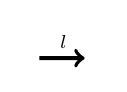
\begin{tikzpicture}[mycfsm]
      % 
      \node[state, draw=none] (zero) [yshift=-4mm, xshift=5mm] {$~$};
      \node[state, draw=none] (one) [right of=zero, xshift=-10mm]   {$~$};
      % 
      \draw (zero) edge[-to,line width=0.5mm] node[above]{$l$} (one)
      ;
 \end{tikzpicture}
 } 
\!\! q'$ for $(q,l,q',\intf)$.

\begin{definition}[Interface decorations]\label{def:IDM}
Let $M=(Q,q_0,\textit{Act},\delta)$ be a CFSM. We define the {\em interface decorations set} of $M$
as the following set of CFSMs with interface edges:
$$\IDS(M) = \Set{(Q,q_0,\textit{Act},\bm{\delta'}) \mid \proj{\bm{\delta'}}{Q\times\textit{Act}\times Q} =\delta}$$
\end{definition}

%\begin{definition}[$\I(M)$]\label{def:IM}%\hfill\\
%Let $M=(Q,q_0,\textit{Act},\bm{\delta})$ be a CFSM with interface edges
%and let $M'=(Q',q'_0,\textit{Act},\delta')$ be a standard CFSM. We say that
%$M'$ is an {\em interface for $M$ via $(f,g)$}, $\I^M_{\!\!(f,g)}(M')$, whenever
%\begin{itemize}
%\item[-]
%$f:Q\to Q'$  is onto and such that, for all $q\in Q$, $\langin(q)=\langin(f(q))$;
%\item[-]
%$g:\delta'\to\Set{e\in\delta\mid e \text{ is an interface edge}}$ is such that 
%$\I(M)$ as the CFSM obtained out of $\bm{\varepsilon}(M)$ using the standard procedure
%to get a FSA without $\varepsilon$-transitions out of a $\varepsilon$-FSA \cite[someStandardReference]. 
%Roughly:\\ 
%- one first calculate the $\varepsilon$-closure for each state, which is the set of all states reachable from a given state using only $\varepsilon$-transitions;\\ 
%- then, for each element of $\textit{Act}$, define new transitions for each state by considering the $\varepsilon$-closures of the states reachable via the original transition function.
%\end{itemize}
%\end{definition}

\begin{definition}[$\roles$-duality]\label{def:PD}%\hfill\\
\begin{enumerate}[i)]
\item
Let $M=(Q,q_0,\textit{Act},\bm{\delta})$ be a CFSM with interface edges. We define
$\bm{\varepsilon}(M)$ as  the $\varepsilon$-FSA $(Q,q_0,\textit{Act}\cup\Set{\varepsilon},\delta')$   where\\
\centerline{
$\delta' = \Set{(q,l,q') \mid (q,l,q',\nintf) \in \bm{\delta}}\cup \Set{(q,\varepsilon,q') \mid (q,l,q',\intf) \in \bm{\delta}}$  }
\item
Let $l,l'\in\textit{Act}\cup\Set{\varepsilon}$ and  let $\roles\neq\emptyset$ be a set of participants.
We say that $l'$ is {\em a $\roles$-dual of $l$} whenever 
\begin{itemize}
\item[-]
$l = \ttr\ttq?\msg[m] \implies l'= \ttq\tts!\msg[m] \text{ with } \tts\in\roles$, $\tts\neq\ttq$;
\item[-]
$l = \ttq\ttr!\msg[m] \implies l'= \tts\ttq?\msg[m] \text{ with } \tts\in\roles$, $\tts\neq\ttq$.
\end{itemize}
\item
Let $\delta,\delta'\in Q\times\textit{Act}\cup\Set{\varepsilon}\times Q$ and  let $\roles$ be a set of participants.
We say that $\delta'$ is {\em a $\roles$-dual of $\delta$} whenever is a minimal relation over
 $Q\times\textit{Act}\cup\Set{\varepsilon}\times Q$ such that\\
\centerline{
$q\lts{l}q'\in\delta \implies q\lts{l'}q'\in\delta'$, where $l'$ is a $\roles$-dual of $l$.
}
\item
Let $M=(Q,q_0,\textit{Act}\cup\Set{\varepsilon},\delta)$ and $M'=(Q,q_0,\textit{Act}\cup\Set{\varepsilon},\delta')$ be two $\varepsilon$-FSA and  let $\roles$ be a set of participants.
We say that $M''$ is {\em a $\roles$-dual of $M$} whenever $\delta'$ is a $\roles$-dual of $\delta$.
\end{enumerate}
\end{definition}

\begin{definition}
%\begin{enumerate}
%\item
%We define the set of the {\em duals of $\delta'$ with respect to} $\roles$  as the following set of $\epsilon$-FSA
%$$\bm{\delta}\text{-}\duals_{\,\roles}(M) = 
%\Set{(Q,q_0,\textit{Act}\cup\Set{\epsilon},\delta'') \mid q\lts{l'}q'\in\delta'' \text{ if } }$$
%where $\bm{\varepsilon}(M) = (Q,q_0,\textit{Act}\cup\Set{\epsilon},\delta')$.
%\item
Let $M=(Q,q_0,\textit{Act}\cup\Set{\varepsilon},\delta)$ be a $\varepsilon$-FSA.
We define $\I(M)$ as the CFSM obtained out of $\bm{\varepsilon}(M)$ 
using the following version of the standard procedure to get a FSA without $\varepsilon$-transitions
out of a $\varepsilon$-FSA \cite{sipser96}, where final states are not taken into account and
the set of states of $\I(M)$ and $\bm{\varepsilon}(M)$ stay the same . 
Roughly:\\ 
- Add an arc from p to q labeled a iff there is an arc labeled a in N from some state in eps-CLOSE(p) to q.;\\
- Delete all arcs labeled with epsilon.
%%- one first calculate the $\varepsilon$-closure for each state, which is the set of all states reachable from a given state using only $\varepsilon$-transitions;\\ 
%%- then, for each element of $\textit{Act}$, define new transitions for each state by considering the $\varepsilon$-closures of the states reachable via the original transition function.
%\end{enumerate}
\end{definition}
%Notice that the states of $\I(M)$ and $M$ are the same.
Mention the fact that we can take any automaton having some specific property w.r.t. $\bm{\varepsilon}(M)$.

We consider $\I(M)$ defined only in case the above construction returns a deterministic automaton.
 

\begin{definition}[$\roles$-complementarity]
Let $M^1_\hh = (Q, q_0, \textit{Act}, \delta^1)$ and 
$M^2_\hh = (Q, q_0, \textit{Act}, \delta^2)$  
be two CFSMs with the same name $\hh$, and let $\roles$ be a set of participants.
Moreover, let $\bm{\delta} \subseteq Q\times\textit{Act}\times Q \times \Set{\intf,\nintf}$
We say that
$M^1_\hh$ is {\em $\roles$-complementary} with $M^2_\hh$ via $\bm{\delta}$, written $\emb{\roles}{\bm{\delta}}{M^1_\hh}{M^2_\hh}$, whenever 
$$M^1_\hh = \bm{\varepsilon}(M''_\hh)$$
for some $M''_\hh$ which is a $\roles$-dual of $M'_\hh= (Q, q_0, \textit{Act}, \bm{\delta})\in\IDS(M^2_\hh)$.
\end{definition}

We write simply $\emb{}{\bm{}}{M^1_\hh}{M^2_\hh}$ whenever
$\roles$ and $\delta$ are clear from the context or ininfluent.




\section{Partial-fusion Composition}

%We make distinct two equal labels when they are used in different transitions. 
%\begin{definition}[$M^+$]
%Let $M = (Q, q_0, \textit{Act}, \delta)$. We define
%$$M^+ = (Q, q_0, \textit{Act}', \delta')$$
%where $\textit{Act}'= \Set{\ttr\tts!\msg[m]^{(q,l,q')},\ttr\tts?\msg[m]^{(q,l,q')} \mid (q,l,q')\in Q\times\textit{Act}\times Q,\ttr,\tts\in\roles, \msg[m] \text{ a message}}$\\
% and 
%$\delta'= \Set{q\lts{\ttr\tts!\msg[m]^{(q,\ttr\tts!\msg[m],q')}}q' \mid q\lts{\ttr\tts!\msg[m]}q'\in\delta}$.
%\end{definition}


%\begin{definition}[$\bm{\delta}$-complementarity]
%Let $M^1_\hh = (Q, q_0, \textit{Act}, \delta^1)$ and $M^2_\hh = (Q, q_0, \textit{Act}, \delta^2)$  be two CFSMs with the same name $\hh$.
%We say that
%\begin{enumerate}[i)]
%\item
%$M^1_\hh$ is {\em $\bm{\delta^2}$-complementary} with $M^2_\hh$, written $\emb{\bm{\delta^2}}{}{M^1_\hh}{M^2_\hh}$, whenever 
%\begin{itemize}
%\item[-] 
%there exists $M'_\hh = (Q, q_0, \textit{Act}, \bm{\delta^2})\in\IDS(M^2_\hh)$;
%\item[-]
%$\I(\bm{\varepsilon}(M'_\hh)^+) = (Q, q_0, \textit{Act}, \delta')$;
%\item[-]
%$q_1 \lts{\hh\ttp!\msg[m]} q_2 \in \delta^1$ for some $\ttp$ \quad iff \quad 
%$q_1\lts{\ttp'\hh?\msg[m]^{(q,l,q')}}q_2\in \delta'$ for some $\ttp'$;
%\item[-]
%$q_1 \lts{\ttp\hh?\msg[m]} q_2 \in \delta^1$ for some $\ttp$ \quad iff \quad 
%$q_1\lts{\hh\ttp'!\msg[m]^{(q,l,q')}}q_2\in \delta'$  for some $\ttp'$;
%
%
%\item[-]
%$q_1\lts{\ttp\hh?\msg[m]^{(q,l,q')}}q_2,q'_1\lts{\ttp\hh?\msg[m]^{(q,l,q')}}q'_2\in \delta'$
%implies
%$q_1 \lts{\hh\ttp'!\msg[m]} q_2, q'_1 \lts{\hh\ttp'!\msg[m]} q'_2 \in \delta^1$;
%\item[-]
%$q_1\lts{\hh\ttp!\msg[m]^{(q,l,q')}}q_2,q'_1\lts{\hh\ttp!\msg[m]^{(q,l,q')}}q'_2\in \delta'$
%implies
%$q_1 \lts{\ttp'\hh?\msg[m]} q_2, q'_1 \lts{\ttp'\hh?\msg[m]} q'_2 \in \delta^1$.
%\end{itemize}
%\end{enumerate}
%\end{definition}
%The fifth and sixth items guarantees that if two labels in $\I(\bm{\varepsilon}(M'_\hh)^+))$ comes
%from the very same transition in $\bm{\varepsilon}(M'_\hh)$ then in $M^1_\hh$ they must
%send(receive) to(from) the same participant.

\begin{definition}[Partial Fusion]
Let $M^1_\hh = (Q^1, q^1_0, \textit{Act}, \delta^1)$ and $M^2_\hh = (Q^2, q^2_0, \textit{Act}, \delta^2)$  be two CFSMs with the same name $\hh$ such that 
$\emb{\bm{\delta}}{\roles\setminus\Set{\hh}}{M^1_{\hh}}{M^2_\hh}$.
We define the {\em partial fusion of $M^1_{\hh}$ and $M^2_{\hh}$ via $\bm{\delta}$ and $\roles$} as
$$\fusion_{\!\!\bm{\delta}}^{\roles}(M^1_{\hh},M^2_{\hh}) = (Q^2\cup\widehat{Q},q_0,\textit{Act},\widehat{\delta})$$
\begin{tabular}{l@{\hspace{1mm}}c@{\hspace{2mm}}l}
where &  $\bullet$  & $\widehat{Q} =\Set{q^{(q, l,q')} \mid (q, l,q',\intf)\in\bm{\delta}}$; \\[1mm]
          &  $\bullet$  & $\widehat\delta = \Set{(q, l,q') \mid (q, l,q',\nintf)\in\bm{\delta}}\,\cup$\\ 
           &    & ${\hspace{20pt}}\Set{(q,\ttr\HH?\msg[a],\widehat q), (\widehat q,\HH\tts!\msg[a],q') \mid  (q,\HH\tts!\msg[a],q',\intf)\in\bm{\delta}, (q,\ttr\hh?\msg[a],\ q')\in\delta^1,\ \widehat q=q^{(q,\HH\tts!\msg[a],q')}}\, \cup$ \\
                &    & ${\hspace{20pt}}\Set{(q,\tts\HH?\msg[a],\widehat q), (\widehat q,\HH'\ttr!\msg[a],q') \mid  (q,\tts\HH?\msg[a],q',\intf)\in\bm{\delta},\ (q,\hh\ttr!\msg[a],q')\in\delta^1,\ \widehat q=q^{(q,\tts\HH?\msg[a],q')}}.$
 \end{tabular} 
\end{definition}



\begin{definition}[Composition by Partial Fusion]
\label{def:cpf}
Let $S_1=(M^1_\ttx)_{\ttx\in\roles_1}$ and $S_2=(M^2_\ttx)_{\ttx\in\roles_2}$ be two communicating systems such that $\roles_1\cap\roles_2=\Set{\hh}$
and $\emb{\bm{\delta}}{\roles_1}{M^1_{\hh}}{M^2_{\hh}}$.
We define the {\em composition of $S_1$ and $S_2$ via partial fusion of $\hh$} by
$$\fusioncomp_{\!\hh}(S_1,S_2) = (\widetilde{M}_\ttx)_{\ttx\in\roles_1\cup\roles_2}$$ 
\begin{tabular}{lc@{\hspace{2mm}}l@{\hspace{4mm}}l}
where &  $\bullet$  & $\widetilde M_\ttx = M^1_\ttx$  & $\text{if}\quad \ttx\in\roles_1 $; \\[1mm]
          &   $\bullet$  & $\widetilde M_\ttx = M^2_\ttx$ &  $\text{if}\quad \ttx\in\roles_2 $; \\[1mm]
                    &   $\bullet$  & $\widetilde M_{\hh} =\fusion_{\!\!\bm{\delta}}^{{\roles_1\setminus\Set{\hh}}}(M^1_{\hh},M^2_{\hh})$.
 \end{tabular} 

\end{definition}

















\section{Composition via partial gateways}

Running example

Let us consider the two following systems $S_1$ and $S_2$ with interfaces, respectively,
$\hh_1$ and $\hh_2$.
\begin{equation}
\label{eq:runex}
\begin{array}{c@{\qquad\qquad}c@{\hspace{1cm}}c@{\hspace{-4mm}}c}
    \begin{array}{cc}
      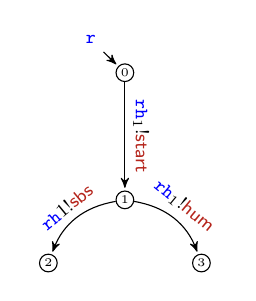
\begin{tikzpicture}[mycfsm]
   \node[state]           (0)                        {$0$};
   \node[draw=none,fill=none] (start) [above left = 0.3cm  of 0]{$\ttr$};
   \node[state]            (1) [below of=0] {$1$};
   \node[state]            (2) [below left of=1, yshift=4mm,xshift=2mm] {$2$};
   \node[state]            (3) [below right of=1, yshift=4mm,xshift=-2mm] {$3$};
%
   \path  (start) edge node {} (0)
            (0)  edge    node [above] {$\ttr\hh_1!\msg[start]$} (1) 
            (1)  edge[bend right]    node [above] {$\ttr\hh1!\msg[sbs]$} (2)
            (1)  edge[bend left]    node [above] {$\ttr\hh_1!\msg[hum]$} (3) 
            ;
       \end{tikzpicture}
&
      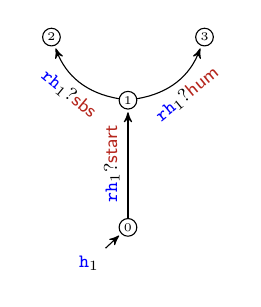
\begin{tikzpicture}[mycfsm]
   \node[state]           (0)                        {$0$};
   \node[draw=none,fill=none] (start) [below left = 0.3cm  of 0]{$\hh_1$};
   \node[state]            (1) [above of=0] {$1$};
   \node[state]            (2) [above left of=1, yshift=-4mm,xshift=2mm] {$2$};
   \node[state]            (3) [above right of=1, yshift=-4mm,xshift=-2mm] {$3$};
%
   \path  (start) edge node {} (0)
            (0)  edge                    node [above] {$\ttr\hh_1?\msg[start]$} (1) 
            (1)  edge[bend left]    node [below] {$\ttr\hh_1?\msg[sbs]$} (2)
            (1)  edge[bend right]    node [below] {$\ttr\hh_1?\msg[hum]$} (3) 
            ;
       \end{tikzpicture}
    \end{array}
       &
       \begin{array}{c}
       |\\
       |\\
       |\\
       |
       \end{array}
       &
      \raisebox{3mm}{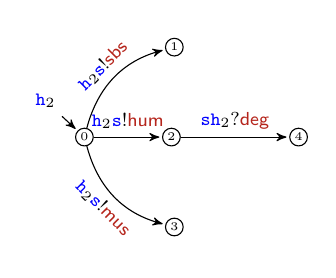
\begin{tikzpicture}[mycfsm]
  \node[state]           (0)              {$0$};
   \node[draw=none,fill=none] (start) [above left = 0.3cm  of 0]{$\hh_2$};
  \node[state]            (1) [above right of=0] {$1$};
   \node[state]           (2) [right of=0,xshift=-6mm] {$2$};
   \node[state]           (3) [below right of=0] {$3$};
   \node[state]           (4) [right of=2] {$4$};
   %
   \path  (start) edge node {} (0) 
            (0)  edge     [bend left]      node [above] {$\hh_2\tts!\msg[sbs]$} (1)
                   edge                          node [above]  {$\hh_2\tts!\msg[hum]$} (2)
                   edge    [bend right]     node [below]  {$\hh_2\tts!\msg[mus]$} (3)
            (2)  edge                           node [above]  {$\tts\hh_2?\msg[deg]$} (4)
                   ;
       \end{tikzpicture}
        }
&
      \raisebox{-3mm}{ 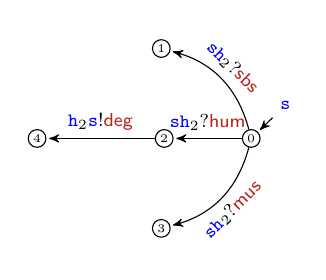
\begin{tikzpicture}[mycfsm]
  \node[state]           (0)            {$0$};
   \node[draw=none,fill=none] (start) [above right = 0.3cm  of 0]{$\tts$};
  \node[state]            (1) [above left of=0] {$1$};
   \node[state]           (2) [left of=0,xshift=6mm] {$2$};
   \node[state]           (3) [below left of=0] {$3$};
   \node[state]           (4) [left of=2] {$4$};
   %
   \path  (start) edge node {} (0) 
            (0)  edge     [bend right]      node [above] {$\tts\hh_2?\msg[sbs]$} (1)
                   edge                          node [above]  {$\tts\hh_2?\msg[hum]$} (2)
                   edge    [bend left]     node [below]  {$\tts\hh_2?\msg[mus]$} (3)
            (2)  edge                           node [above]  {$\hh_2\tts!\msg[deg]$} (4)
                   ;
       \end{tikzpicture}
       }
\end{array}
\end{equation}

$S_1$ and $S_2$ are both deadlock free and both enjoy the progress property.

Transforming $\hh_1$ and $\hh_2$ into gateways make the resulting composition non
deadlock free.
In fact, the (unique) connection policy is as below, and it is non deadlock free.

$$
\dbox{
     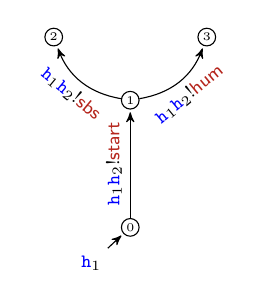
\begin{tikzpicture}[mycfsm]
   \node[state]           (0)                        {$0$};
   \node[draw=none,fill=none] (start) [below left = 0.3cm  of 0]{$\hh_1$};
   \node[state]            (1) [above of=0] {$1$};
   \node[state]            (2) [above left of=1, yshift=-4mm,xshift=2mm] {$2$};
   \node[state]            (3) [above right of=1, yshift=-4mm,xshift=-2mm] {$3$};
%
   \path  (start) edge node {} (0)
            (0)  edge                    node [above] {$\hh_1\hh_2!\msg[start]$} (1) 
            (1)  edge[bend left]    node [below] {$\hh_1\hh_2!\msg[sbs]$} (2)
            (1)  edge[bend right]    node [below] {$\hh_1\hh_2!\msg[hum]$} (3) 
            ;
       \end{tikzpicture}
       \qquad
     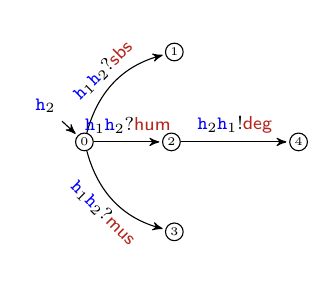
\begin{tikzpicture}[mycfsm]
  \node[state]           (0)              {$0$};
   \node[draw=none,fill=none] (start) [above left = 0.3cm  of 0]{$\hh_2$};
  \node[state]            (1) [above right of=0] {$1$};
   \node[state]           (2) [right of=0,xshift=-6mm] {$2$};
   \node[state]           (3) [below right of=0] {$3$};
   \node[state]           (4) [right of=2] {$4$};
   %
   \path  (start) edge node {} (0) 
            (0)  edge     [bend left]      node [above] {$\hh_1\hh_2?\msg[sbs]$} (1)
                   edge                          node [above]  {$\hh_1\hh_2?\msg[hum]$} (2)
                   edge    [bend right]     node [below]  {$\hh_1\hh_2?\msg[mus]$} (3)
            (2)  edge                           node [above]  {$\hh_2\hh_1!\msg[deg]$} (4)
                   ;
       \end{tikzpicture}
}
$$

Instead of looking at a whole participant as an interface, we can 
consider only specific edges as description of actions of an outer system.
In our running example, for instance, we could still decide to compose $S_1$ and $S_2$ trough
$\hh_1$ and $\hh_2$, proviso that only the edges in bold in the drawing below
have to be interpreted as actions of the outer systems one intend to be connected to.  


\begin{equation}
\label{eq:1}
\begin{array}{c@{\qquad}c@{\hspace{1cm}}c@{\hspace{-4mm}}c}
    \begin{array}{cc}
      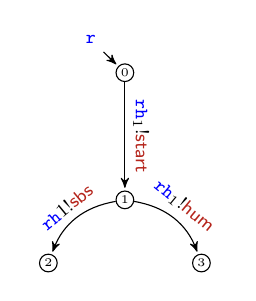
\begin{tikzpicture}[mycfsm]
   \node[state]           (0)                        {$0$};
   \node[draw=none,fill=none] (start) [above left = 0.3cm  of 0]{$\ttr$};
   \node[state]            (1) [below of=0] {$1$};
   \node[state]            (2) [below left of=1, yshift=4mm,xshift=2mm] {$2$};
   \node[state]            (3) [below right of=1, yshift=4mm,xshift=-2mm] {$3$};
%
   \path  (start) edge node {} (0)
            (0)  edge    node [above] {$\ttr\hh_1!\msg[start]$} (1) 
            (1)  edge[bend right]    node [above] {$\ttr\hh1!\msg[sbs]$} (2)
            (1)  edge[bend left]    node [above] {$\ttr\hh_1!\msg[hum]$} (3) 
            ;
       \end{tikzpicture}
&
      \begin{tikzpicture}[mycfsm]
   \node[state]           (0)                        {$0$};
   \node[draw=none,fill=none] (start) [below left = 0.3cm  of 0]{$\hh_1$};
   \node[state]            (1) [above of=0] {$1$};
   \node[state]            (2) [above left of=1, yshift=-4mm,xshift=2mm] {$2$};
   \node[state]            (3) [above right of=1, yshift=-4mm,xshift=-2mm] {$3$};
%
   \path  (start) edge node {} (0)
            (0)  edge                    node [above] {$\ttr\hh_1?\msg[start]$} (1) 
            (1)  edge[bend left, line width=0.5mm]    node [below] {$\ttr\hh_1?\msg[sbs]$} (2)
            (1)  edge[bend right, line width=0.5mm]    node [below] {$\ttr\hh_1?\msg[hum]$} (3) 
            ;
       \end{tikzpicture}
    \end{array}
       &
       \begin{array}{c}
       |\\
       |\\
       |\\
       |
       \end{array}
       &
      \raisebox{3mm}{\begin{tikzpicture}[mycfsm]
  \node[state]           (0)              {$0$};
   \node[draw=none,fill=none] (start) [above left = 0.3cm  of 0]{$\hh_2$};
  \node[state]            (1) [above right of=0] {$1$};
   \node[state]           (2) [right of=0,xshift=-6mm] {$2$};
   \node[state]           (3) [below right of=0] {$3$};
   \node[state]           (4) [right of=2] {$4$};
   %
   \path  (start) edge node {} (0) 
            (0)  edge     [bend left, line width=0.5mm]      node [above] {$\hh_2\tts!\msg[sbs]$} (1)
                   edge     [line width=0.5mm]                     node [above]  {$\hh_2\tts!\msg[hum]$} (2)
                   edge    [bend right, line width=0.5mm]     node [below]  {$\hh_2\tts!\msg[mus]$} (3)
            (2)  edge                           node [above]  {$\tts\hh_2?\msg[deg]$} (4)
                   ;
       \end{tikzpicture}
        }
&
      \raisebox{-3mm}{ \begin{tikzpicture}[mycfsm]
  \node[state]           (0)            {$0$};
   \node[draw=none,fill=none] (start) [above right = 0.3cm  of 0]{$\tts$};
  \node[state]            (1) [above left of=0] {$1$};
   \node[state]           (2) [left of=0,xshift=6mm] {$2$};
   \node[state]           (3) [below left of=0] {$3$};
   \node[state]           (4) [left of=2] {$4$};
   %
   \path  (start) edge node {} (0) 
            (0)  edge     [bend right]      node [above] {$\tts\hh_2?\msg[sbs]$} (1)
                   edge                          node [above]  {$\tts\hh_2?\msg[hum]$} (2)
                   edge    [bend left]     node [below]  {$\tts\hh_2?\msg[mus]$} (3)
            (2)  edge                           node [above]  {$\hh_2\tts!\msg[deg]$} (4)
                   ;
       \end{tikzpicture}
       }
\end{array}
\end{equation}

The connection policy has now to be formed by CFSM describing the interactions 
between the ``interface'' parts of $\hh_1$ and $\hh_2$, which in our running examples 
turn out to be simply as follows.

\begin{equation}
\label{eq:cp1}
\dbox{
     \begin{tikzpicture}[mycfsm]
   \node[state]            (1) [above of=0] {$1$};
   \node[draw=none,fill=none] (start) [below left = 0.3cm  of 1]{$\hh_1$};
   \node[state]            (2) [above left of=1, yshift=-4mm,xshift=2mm] {$2$};
   \node[state]            (3) [above right of=1, yshift=-4mm,xshift=-2mm] {$3$};
%
   \path  (start) edge node {} (1)
            (1)  edge[bend left]    node [below] {$\hh_1\hh_2!\msg[sbs]$} (2)
            (1)  edge[bend right]    node [below] {$\hh_1\hh_2!\msg[hum]$} (3) 
            ;
       \end{tikzpicture}
       \qquad
     \begin{tikzpicture}[mycfsm]
  \node[state]           (0)              {$0$};
   \node[draw=none,fill=none] (start) [above left = 0.3cm  of 0]{$\hh_2$};
  \node[state]            (1) [above right of=0] {$1$};
   \node[state]           (2) [right of=0,xshift=-6mm] {$2$};
   \node[state]           (3) [below right of=0] {$3$};
   %
   \path  (start) edge node {} (0) 
            (0)  edge     [bend left]      node [above] {$\hh_1\hh_2?\msg[sbs]$} (1)
                   edge                          node [above]  {$\hh_1\hh_2?\msg[hum]$} (2)
                   edge    [bend right]     node [below]  {$\hh_1\hh_2?\msg[mus]$} (3)
                   ;
       \end{tikzpicture}
}
\end{equation}

Such a communicating system does enjoy all communication properties we considered.

The partial gateways have to act as forwarders only for what concerns the interface parts,
whereas non interface parts describe what is still in charge of the participants $\hh_1$ and $\hh_2$.
A partial gateway is hence built out of an interface machine and its counterpart in the
communication policy we intend to use for the composition. 
 \vspace{-1mm} In particular, out of the interface transition
\raisebox{2mm}
{\begin{tikzpicture}[mycfsm]
      % 
      \node[state] (zero) [yshift=-4mm] {$0$};
      \node[state] (one) [right of=zero, xshift=-2mm]   {$1$};
      % 
      \path
      (zero) edge[bend left=15, line width=0.5mm] node[above] {$\aout[h_2][s][][sbs]$} (one)
      ;
 \end{tikzpicture}
 } 
 of $\hh_2$ in (\ref{eq:1}) and of the transition
 \raisebox{2mm}
{\begin{tikzpicture}[mycfsm]
      % 
      \node[state] (zero) [yshift=-4mm] {$0$};
      \node[state] (one) [right of=zero, xshift=-2mm]   {$1$};
      % 
      \path
      (zero) edge[bend left=15] node[above] {$\ain[\hh_2][\hh_2][][sbs]$} (one)
      ;
 \end{tikzpicture}
 }  
 of $\hh_2$ in the connection policy (\ref{eq:cp1}) , we introduce 
  \raisebox{2mm}
{\begin{tikzpicture}[mycfsm]
      % 
      \node[state] (zero) [yshift=-4mm] {$0$};
      \node[state] (one) [right of=zero, xshift=-2mm, yshift=2mm]   {$\widehat 1$};
       \node[state] (two) [right of=one, xshift=-2mm, yshift=-2mm,]   {$1$};
      % 
      \path
      (zero) edge[bend left=10] node[above] {$\ain[h_1][h_2][][sbs]$} (one)
      (one) edge[bend left=10] node[above] {$\aout[\hh_2][s][][sbs]$} (two)
      ;
 \end{tikzpicture}
 }
in the resulting partial gateway, where the $\widehat 1$ stated is specifically introduced 
by the partial gateway construction.
Recall that, in order to enforce conservativity, gateways are given the same names as the
corresponding interfaces.
The above discussion applies, dually, for edges in the interface $\hh_1$ labelled with output actions.
Non interface transitions are left unchanged by the partial gateway construction.



So, the resulting composed system is as follows.

$$
\begin{array}{cc@{\hspace{-4mm}}c}
    \begin{array}{cc}
      \begin{tikzpicture}[mycfsm]
   \node[state]           (0)                        {$0$};
   \node[draw=none,fill=none] (start) [above left = 0.3cm  of 0]{$\ttr$};
   \node[state]            (1) [below of=0] {$1$};
   \node[state]            (2) [below left of=1, yshift=4mm,xshift=2mm] {$2$};
   \node[state]            (3) [below right of=1, yshift=4mm,xshift=-2mm] {$3$};
%
   \path  (start) edge node {} (0)
            (0)  edge    node [above] {$\ttr\hh_1!\msg[start]$} (1) 
            (1)  edge[bend right]    node [above] {$\ttr\hh1!\msg[sbs]$} (2)
            (1)  edge[bend left]    node [above] {$\ttr\hh_1!\msg[hum]$} (3) 
            ;
       \end{tikzpicture}
&
      \begin{tikzpicture}[mycfsm]
   \node[state]           (0)                        {$0$};
   \node[draw=none,fill=none] (start) [below left = 0.3cm  of 0]{$\hh_1$};
   \node[state]            (1) [above of=0] {$1$};
   \node[state]            (1hat) [above left of=1, yshift=-4mm,xshift=2mm] {$\widehat 1$};
   \node[state]            (2) [above of=1hat, yshift=-2mm] {$2$};
   \node[state]            (2hat) [above right of=1, yshift=-4mm,xshift=-2mm] {$\widehat 2$};
   \node[state]            (3) [above of=2hat, yshift=-2mm] {$3$};
%
   \path  (start) edge node {} (0)
            (0)  edge                    node [above] {$\ttr\hh_1?\msg[start]$} (1) 
            (1)  edge[bend left]    node [below] {$\ttr\hh_1?\msg[sbs]$} (1hat)
             (1hat)  edge   node [below] {$\hh_1\hh_2!\msg[sbs]$} (2)
            (1)  edge[bend right]    node [below] {$\ttr\hh_1?\msg[hum]$} (2hat) 
             (2hat)  edge   node [below] {$\hh_1\hh_2!\msg[hum]$} (3) 
            ;
       \end{tikzpicture}
    \end{array}
  &
      \raisebox{3mm}{\begin{tikzpicture}[mycfsm]
  \node[state]           (0)              {$0$};
   \node[draw=none,fill=none] (start) [above left = 0.3cm  of 0]{$\hh_2$};
  \node[state]            (1hat) [above right of=0] {$\widehat 1$};
    \node[state]            (1) [right of=1hat] {$1$};
   \node[state]           (2hat) [right of=0,xshift=-6mm] {$\widehat 2$};
    \node[state]           (2) [right of=2hat] {$2$};
   \node[state]           (3hat) [below right of=0] {$\widehat 3$};
   \node[state]           (3) [ right of=3hat] {$3$};
   \node[state]           (4) [right of=2] {$4$};
   %
   \path  (start) edge node {} (0) 
            (0)  edge     [bend left]      node [above] {$\hh_1\hh_2?\msg[sbs]$} (1hat)
                   edge                          node [above]  {$\hh_1\hh_2?\msg[hum]$} (2hat)
                   edge    [bend right]     node [below]  {$\hh_1\hh_2?\msg[mus]$} (3hat)
            (3hat)  edge                      node [below]  {$\hh_2\tts!\msg[mus]$} (3)
            (1hat)  edge                      node [above]  {$\hh_2\tts!\msg[sbs]$} (1)
            (2hat)  edge                      node [above]  {$\hh_2\tts!\msg[hum]$} (2)
            (2)  edge                           node [above]  {$\tts\hh_2?\msg[deg]$} (4)
                   ;
       \end{tikzpicture}
        }
&
      \raisebox{-3mm}{ \begin{tikzpicture}[mycfsm]
  \node[state]           (0)            {$0$};
   \node[draw=none,fill=none] (start) [above right = 0.3cm  of 0]{$\tts$};
  \node[state]            (1) [above left of=0] {$1$};
   \node[state]           (2) [left of=0,xshift=6mm] {$2$};
   \node[state]           (3) [below left of=0] {$3$};
   \node[state]           (4) [left of=2] {$4$};
   %
   \path  (start) edge node {} (0) 
            (0)  edge     [bend right]      node [above] {$\tts\hh_2?\msg[sbs]$} (1)
                   edge                          node [above]  {$\tts\hh_2?\msg[hum]$} (2)
                   edge    [bend left]     node [below]  {$\tts\hh_2?\msg[mus]$} (3)
            (2)  edge                           node [above]  {$\hh_2\tts!\msg[deg]$} (4)
                   ;
       \end{tikzpicture}
       }
\end{array}
$$

Our result will allow to infer that in this particular case the composition via partial gateways
satisfies also the communication properties (but lock-freedom).

Some care has however to be taken when, onece choosen the participants playing the roles of 
partial interfaces,  we decide which are the interface edge.
It is in fact not possible to consider any edge as an interface edge.

Let us consider again our running example, and let us consider again $\hh_1$ and 
$\hh_2$ as (partial) interfaces. However, let us consider now the following interface edges.



%We hence introduce the notion of CFSM with interface edges. 

 \begin{equation}
 \label{eq:2}
\begin{array}{c@{\qquad}c@{\hspace{1cm}}c@{\hspace{-4mm}}c}
    \begin{array}{cc}
      \begin{tikzpicture}[mycfsm]
   \node[state]           (0)                        {$0$};
   \node[draw=none,fill=none] (start) [above left = 0.3cm  of 0]{$\ttr$};
   \node[state]            (1) [below of=0] {$1$};
   \node[state]            (2) [below left of=1, yshift=4mm,xshift=2mm] {$2$};
   \node[state]            (3) [below right of=1, yshift=4mm,xshift=-2mm] {$3$};
%
   \path  (start) edge node {} (0)
            (0)  edge    node [above] {$\ttr\hh_1!\msg[start]$} (1) 
            (1)  edge[bend right]    node [above] {$\ttr\hh1!\msg[sbs]$} (2)
            (1)  edge[bend left]    node [above] {$\ttr\hh_1!\msg[hum]$} (3) 
            ;
       \end{tikzpicture}
&
      \begin{tikzpicture}[mycfsm]
   \node[state]           (0)                        {$0$};
   \node[draw=none,fill=none] (start) [below left = 0.3cm  of 0]{$\hh_1$};
   \node[state]            (1) [above of=0] {$1$};
   \node[state]            (2) [above left of=1, yshift=-4mm,xshift=2mm] {$2$};
   \node[state]            (3) [above right of=1, yshift=-4mm,xshift=-2mm] {$3$};
%
   \path  (start) edge node {} (0)
            (0)  edge                    node [above] {$\ttr\hh_1?\msg[start]$} (1) 
            (1)  edge[bend left, line width=0.5mm]    node [below] {$\ttr\hh_1?\msg[sbs]$} (2)
            (1)  edge[bend right, line width=0.5mm]    node [below] {$\ttr\hh_1?\msg[hum]$} (3) 
            ;
       \end{tikzpicture}
    \end{array}
       &
       \begin{array}{c}
       |\\
       |\\
       |\\
       |
       \end{array}
       &
      \raisebox{3mm}{\begin{tikzpicture}[mycfsm]
  \node[state]           (0)              {$0$};
   \node[draw=none,fill=none] (start) [above left = 0.3cm  of 0]{$\hh_2$};
  \node[state]            (1) [above right of=0] {$1$};
   \node[state]           (2) [right of=0,xshift=-6mm] {$2$};
   \node[state]           (3) [below right of=0] {$3$};
   \node[state]           (4) [right of=2] {$4$};
   %
   \path  (start) edge node {} (0) 
            (0)  edge     [bend left, line width=0.5mm]      node [above] {$\hh_2\tts!\msg[sbs]$} (1)
                   edge     [line width=0.5mm]                     node [above]  {$\hh_2\tts!\msg[hum]$} (2)
                   edge    [bend right]     node [below]  {$\hh_2\tts!\msg[mus]$} (3)
            (2)  edge                           node [above]  {$\tts\hh_2?\msg[deg]$} (4)
                   ;
       \end{tikzpicture}
        }
&
      \raisebox{-3mm}{ \begin{tikzpicture}[mycfsm]
  \node[state]           (0)            {$0$};
   \node[draw=none,fill=none] (start) [above right = 0.3cm  of 0]{$\tts$};
  \node[state]            (1) [above left of=0] {$1$};
   \node[state]           (2) [left of=0,xshift=6mm] {$2$};
   \node[state]           (3) [below left of=0] {$3$};
   \node[state]           (4) [left of=2] {$4$};
   %
   \path  (start) edge node {} (0) 
            (0)  edge     [bend right]      node [above] {$\tts\hh_2?\msg[sbs]$} (1)
                   edge                          node [above]  {$\hh_2\tts!\msg[hum]$} (2)
                   edge    [bend left]     node [below]  {$\hh_2\tts!\msg[mus]$} (3)
            (2)  edge                           node [above]  {$\hh_2\tts!\msg[deg]$} (4)
                   ;
       \end{tikzpicture}
       }
\end{array}
\end{equation}

The corresponding connection policy is 

$$
\dbox{
     \begin{tikzpicture}[mycfsm]
   \node[state]            (1) [above of=0] {$1$};
   \node[draw=none,fill=none] (start) [below left = 0.3cm  of 1]{$\hh_1$};
   \node[state]            (2) [above left of=1, yshift=-4mm,xshift=2mm] {$2$};
   \node[state]            (3) [above right of=1, yshift=-4mm,xshift=-2mm] {$3$};
%
   \path  (start) edge node {} (1)
            (1)  edge[bend left]    node [below] {$\hh_1\hh_2!\msg[sbs]$} (2)
            (1)  edge[bend right]    node [below] {$\hh_1\hh_2!\msg[hum]$} (3) 
            ;
       \end{tikzpicture}
       \qquad
     \begin{tikzpicture}[mycfsm]
  \node[state]           (0)              {$0$};
   \node[draw=none,fill=none] (start) [above left = 0.3cm  of 0]{$\hh_2$};
  \node[state]            (1) [above right of=0, xshift=1mm] {$1$};
   \node[state]           (2) [right of=0, xshift=-4.5mm] {$2$};
   %
   \path  (start) edge node {} (0) 
            (0)  edge     [bend left]      node [above] {$\hh_1\hh_2?\msg[sbs]$} (1)
                   edge                          node [below]  {$\hh_1\hh_2?\msg[hum]$} (2)
                   ;
       \end{tikzpicture}
}
$$
This communicating system is orphan-message free.

 The composition obtaining by building partial gateways of such connection policy is then the 
 following communication system.

\begin{equation}
\label{eq:comprunex}
\begin{array}{cc@{\hspace{-4mm}}c}
    \begin{array}{cc}
      \begin{tikzpicture}[mycfsm]
   \node[state]           (0)                        {$0$};
   \node[draw=none,fill=none] (start) [above left = 0.3cm  of 0]{$\ttr$};
   \node[state]            (1) [below of=0] {$1$};
   \node[state]            (2) [below left of=1, yshift=4mm,xshift=2mm] {$2$};
   \node[state]            (3) [below right of=1, yshift=4mm,xshift=-2mm] {$3$};
%
   \path  (start) edge node {} (0)
            (0)  edge    node [above] {$\ttr\hh_1!\msg[start]$} (1) 
            (1)  edge[bend right]    node [above] {$\ttr\hh1!\msg[sbs]$} (2)
            (1)  edge[bend left]    node [above] {$\ttr\hh_1!\msg[hum]$} (3) 
            ;
       \end{tikzpicture}
&
      \begin{tikzpicture}[mycfsm]
   \node[state]           (0)                        {$0$};
   \node[draw=none,fill=none] (start) [below left = 0.3cm  of 0]{$\hh_1$};
   \node[state]            (1) [above of=0] {$1$};
   \node[state]            (1hat) [above left of=1, yshift=-4mm,xshift=2mm] {$\widehat 1$};
   \node[state]            (2) [above of=1hat, yshift=-2mm] {$2$};
   \node[state]            (2hat) [above right of=1, yshift=-4mm,xshift=-2mm] {$\widehat 2$};
   \node[state]            (3) [above of=2hat, yshift=-2mm] {$3$};
%
   \path  (start) edge node {} (0)
            (0)  edge                    node [above] {$\ttr\hh_1?\msg[start]$} (1) 
            (1)  edge[bend left]    node [below] {$\ttr\hh_1?\msg[sbs]$} (1hat)
             (1hat)  edge   node [below] {$\hh_1\hh_2!\msg[sbs]$} (2)
            (1)  edge[bend right]    node [below] {$\ttr\hh_1?\msg[hum]$} (2hat) 
             (2hat)  edge   node [below] {$\hh_1\hh_2!\msg[hum]$} (3) 
            ;
       \end{tikzpicture}
    \end{array}
  &
      \raisebox{3mm}{\begin{tikzpicture}[mycfsm]
  \node[state]           (0)              {$0$};
   \node[draw=none,fill=none] (start) [above left = 0.3cm  of 0]{$\hh_2$};
  \node[state]            (1hat) [above right of=0] {$\widehat 1$};
    \node[state]            (1) [right of=1hat] {$1$};
   \node[state]           (2hat) [right of=0,xshift=-6mm] {$\widehat 2$};
    \node[state]           (2) [right of=2hat] {$2$};
   \node[state]           (3) [below right of=0] {$3$};
   \node[state]           (4) [right of=2] {$4$};
   %
   \path  (start) edge node {} (0) 
            (0)  edge     [bend left]      node [above] {$\hh_1\hh_2?\msg[sbs]$} (1hat)
                   edge                          node [above]  {$\hh_1\hh_2?\msg[hum]$} (2hat)
                   edge    [bend right]     node [below]  {$\hh_2\tts!\msg[mus]$} (3)
            (1hat)  edge                      node [above]  {$\hh_2\tts!\msg[sbs]$} (1)
            (2hat)  edge                      node [above]  {$\hh_2\tts!\msg[hum]$} (2)
            (2)  edge                           node [above]  {$\tts\hh_2?\msg[deg]$} (4)
                   ;
       \end{tikzpicture}
        }
&
      \raisebox{-3mm}{ \begin{tikzpicture}[mycfsm]
  \node[state]           (0)            {$0$};
   \node[draw=none,fill=none] (start) [above right = 0.3cm  of 0]{$\tts$};
  \node[state]            (1) [above left of=0] {$1$};
   \node[state]           (2) [left of=0,xshift=6mm] {$2$};
   \node[state]           (3) [below left of=0] {$3$};
   \node[state]           (4) [left of=2] {$4$};
   %
   \path  (start) edge node {} (0) 
            (0)  edge     [bend right]      node [above] {$\tts\hh_2?\msg[sbs]$} (1)
                   edge                          node [above]  {$\tts\hh_2?\msg[hum]$} (2)
                   edge    [bend left]     node [below]  {$\tts\hh_2?\msg[mus]$} (3)
            (2)  edge                           node [above]  {$\hh_2\tts!\msg[deg]$} (4)
                   ;
       \end{tikzpicture}
       }
\end{array}
\end{equation}

Scuh communicating system, however, is not orphan-message free.
In fact the following configuration, made by final states only, is reachable:\\
\centerline{
$s=((3_\ttr,3_{\hh_1},3_{\hh_2},3_\tts),\vec{w})$
}
where $\vec{w}\neq\vec{\varepsilon}$, in particular $w_{\hh_1\hh_2}=\langle\msg[hum]\rangle$.\\
Hence $s$ is an orphan-message configuration.

A similar choice of interface edges can disrupt progress preservation.
 
Let us consider the two following systems $S_1$ and $S_2$ with interfaces, respectively,
$\hh_1$ and $\hh_2$. Both satisfying the progress property.
\begin{equation}
\label{eq:3}
\begin{array}{c@{\qquad}c@{\hspace{1cm}}c@{\qquad}c}
    \begin{array}{cc}
      \begin{tikzpicture}[mycfsm]
  \node[state]           (0)                        {$0$};
   \node[draw=none,fill=none] (start) [above left = 0.3cm  of 0]{$\ttu$};
   \node[state]            (1) [below of=0, yshift=4mm] {$1$};

   \path  (start) edge node {} (0)
            (0)  edge    node [above] {$\hh_1\ttu?\msg[a]$} (1) ;
       \end{tikzpicture}
&
       \begin{tikzpicture}[mycfsm]
  \node[state]           (0)                        {$0$};
   \node[draw=none,fill=none] (start) [above left = 0.3cm  of 0]{$\hh_1$};
  \node[state]            (1) [right of=0] {$1$};
  %\node[state]           (2) [above right of=0] {$2$};

   \path  (start) edge node {} (0) 
            (0)  edge [line width=0.5mm]     node [below] {$\hh_1\ttu!\msg[a]$} (1);
       \end{tikzpicture}
    \end{array}
       &
       \begin{array}{c}
       |\\
       |\\
       |\\
       |
       \end{array}
       &
       \begin{tikzpicture}[mycfsm]
  \node[state]           (0)                        {$0$};
   \node[draw=none,fill=none] (start) [above left = 0.3cm  of 0]{$\hh_2$};
  \node[state]            (1) [above right of=0,yshift=-5mm] {$1$};
  \node[state]           (2) [below right of=0,yshift=5mm] {$2$};

   \path  (start) edge node {} (0) 
            (0)  edge     [bend left]      node [above] {$\ttv\hh_2?\msg[b]$} (1)
            (0)   edge    [bend right, line width=0.5mm]            node [above]  {$\ttv\hh_2?\msg[a]$} (2);
       \end{tikzpicture}
&
      \begin{tikzpicture}[mycfsm]
  \node[state]           (0)                        {$0$};
   \node[draw=none,fill=none] (start) [above left = 0.3cm  of 0]{$\ttv$};
   \node[state]            (1) [below of=0, yshift=4mm] {$1$};

   \path  (start) edge node {} (0)
            (0)  edge    node [above] {$\ttv\hh_2!\msg[b]$} (1) ;
       \end{tikzpicture}
\end{array}
\end{equation}

The (unique) connection policy below satisfies the progress property.
 
$$
\dbox{
       \begin{tikzpicture}[mycfsm]
  \node[state]           (0)                        {$0$};
   \node[draw=none,fill=none] (start) [above left = 0.3cm  of 0]{$\hh_1$};
  \node[state]            (1) [right of=0] {$1$};
%
   \path  (start) edge node {} (0) 
            (0)  edge [line width=0.5mm]     node [below] {$\hh_2\hh_1?\msg[a]$} (1);
       \end{tikzpicture}
\quad
       \begin{tikzpicture}[mycfsm]
  \node[state]           (0)                        {$0$};
   \node[draw=none,fill=none] (start) [above left = 0.3cm  of 0]{$\hh_2$};
  \node[state]           (2) [below right of=0,yshift=5mm] {$2$};

   \path  (start) edge node {} (0)
            (0)   edge    [bend right, line width=0.5mm]            node [above]  {$\hh_2\hh_1!\msg[a]$} (2);
       \end{tikzpicture}
       }
$$

The following composition via partial gateway, however, does not satisfies the progress property.
$$
      \begin{tikzpicture}[mycfsm]
  \node[state]           (0)                        {$0$};
   \node[draw=none,fill=none] (start) [above left = 0.3cm  of 0]{$\ttu$};
   \node[state]            (1) [below of=0, yshift=4mm] {$1$};
%
   \path  (start) edge node {} (0)
            (0)  edge    node [above] {$\hh\ttu?\msg[a]$} (1) ;
       \end{tikzpicture}
\quad
        \begin{tikzpicture}[mycfsm]
  \node[state]           (0)                        {$0$};
   \node[draw=none,fill=none] (start) [above left = 0.3cm  of 0]{$\hh_1$};
  \node[state]            (0hat) [right of=0] {$\widehat 0$};
  \node[state]           (1) [above of=0hat] {$1$};
%
   \path  (start) edge node {} (0) 
            (0)  edge     node [below] {$\hh_2\hh_1?\msg[a]$} (0hat)
            (0hat)  edge     node [below] {$\hh_1\ttu!\msg[a]$} (1)
            ;
       \end{tikzpicture}
\quad
            \begin{tikzpicture}[mycfsm]
  \node[state]           (0)                        {$0$};
  \node[state]           (hat0)          [below right of=0, yshift=5mm]              {$\widehat{0}$};
   \node[draw=none,fill=none] (start) [above left = 0.3cm  of 0]{$\HH_2$};
  \node[state]            (2) [right of=hat0] {$2$};
  \node[state]           (1) [above right of=0, yshift=-5mm] {$1$};
  %\node[state]           (2) [right of=hat0'] {$2$};

   \path  (start) edge node {} (0) 
            (0)         edge   [bend right]        node [below] {${\ttv\hh_2}?{\msg[a]}$} (hat0)
                         edge   [bend left]      node [above]  {${\ttv\hh_2}?{\msg[b]}$} (1)
             (hat0)  edge        node [below] {${\HH_2\hh_1}!{\msg[a]}$} (2);       
             \end{tikzpicture}
\quad
      \begin{tikzpicture}[mycfsm]
  \node[state]           (0)                        {$0$};
   \node[draw=none,fill=none] (start) [above left = 0.3cm  of 0]{$\ttv$};
   \node[state]            (1) [below of=0, yshift=4mm] {$1$};

   \path  (start) edge node {} (0)
            (0)  edge    node [above] {$\ttv\hh_2!\msg[b]$} (1) ;
       \end{tikzpicture}
$$
In fact, some states in $s=(0_\ttu,0_{\hh_1},1_{\hh_2},1_\ttv)$ are not final, $s$ is reachable and $s\notlts{}$. 

The previous two examples, where some properties are not preserved by composition via
partial gateways, share the fact that interfaces have a state with normal and interface outgoing
transitions.
  
The following example shows that progress preservation can be disrupted also in presence of
states all with non interface transitions.

Let us consider the following communicating system.
\begin{equation}
\label{eq:4}
\begin{array}{c@{\qquad}c@{\hspace{1cm}}c@{\qquad}c}
    \begin{array}{cc}
      \begin{tikzpicture}[mycfsm]
  \node[state]           (0)                        {$0$};
   \node[draw=none,fill=none] (start) [above left = 0.3cm  of 0]{$\ttu$};
   \node[state]            (1) [below of=0, yshift=4mm] {$1$};

   \path  (start) edge node {} (0)
            (0)  edge    node [above] {$\hh_1\ttu?\msg[a]$} (1) ;
       \end{tikzpicture}
&
       \begin{tikzpicture}[mycfsm]
  \node[state]           (0)                        {$0$};
   \node[draw=none,fill=none] (start) [above left = 0.3cm  of 0]{$\hh_1$};
  \node[state]            (1) [right of=0] {$1$};
  %\node[state]           (2) [above right of=0] {$2$};

   \path  (start) edge node {} (0) 
            (0)  edge  [line width=0.5mm]     node [below] {$\hh_1\ttu!\msg[a]$} (1);
       \end{tikzpicture}
    \end{array}
       &
       \begin{array}{c}
       |\\
       |\\
       |\\
       |
       \end{array}
       &
       \begin{tikzpicture}[mycfsm]
  \node[state]           (0)                        {$0$};
   \node[draw=none,fill=none] (start) [above left = 0.3cm  of 0]{$\hh_2$};
  \node[state]            (1) [above right of=0,yshift=-5mm] {$1$};
  \node[state]           (2) [below right of=0,yshift=5mm] {$2$};
  \node[state]           (3) [right of=2] {$3$};
%
   \path  (start) edge node {} (0) 
            (0)  edge     [bend left]      node [above] {$\ttv\hh_2?\msg[b]$} (1)
            (0)   edge    [bend right]            node [above]  {$\ttv\hh_2?\msg[c]$} (2)
            (2)   edge    [line width=0.5mm]            node [above]  {$\ttv\hh_2?\msg[a]$} (3);
       \end{tikzpicture}
&
      \begin{tikzpicture}[mycfsm]
  \node[state]           (0)                        {$0$};
   \node[draw=none,fill=none] (start) [above left = 0.3cm  of 0]{$\ttv$};
   \node[state]            (1) [below of=0, yshift=4mm] {$1$};

   \path  (start) edge node {} (0)
            (0)  edge    node [above] {$\ttv\hh_2!\msg[b]$} (1) ;
       \end{tikzpicture}
\end{array}
\end{equation}
The (unique) connection policy satisfies progress.
The composition below, however, does not.
$$
      \begin{tikzpicture}[mycfsm]
  \node[state]           (0)                        {$0$};
   \node[draw=none,fill=none] (start) [above left = 0.3cm  of 0]{$\ttu$};
   \node[state]            (1) [below of=0, yshift=4mm] {$1$};

   \path  (start) edge node {} (0)
            (0)  edge    node [above] {$\hh\ttu?\msg[a]$} (1) ;
       \end{tikzpicture}
\quad
        \begin{tikzpicture}[mycfsm]
  \node[state]           (0)                        {$0$};
   \node[draw=none,fill=none] (start) [above left = 0.3cm  of 0]{$\hh_1$};
  \node[state]            (0hat) [right of=0] {$\widehat 0$};
  \node[state]           (1) [above of=0hat] {$1$};
%
   \path  (start) edge node {} (0) 
            (0)  edge     node [below] {$\hh_2\hh_1?\msg[a]$} (0hat)
            (0hat)  edge     node [below] {$\hh_1\ttu!\msg[a]$} (1)
            ;
       \end{tikzpicture}
\quad
       \begin{tikzpicture}[mycfsm]
  \node[state]           (0)                        {$0$};
   \node[draw=none,fill=none] (start) [above left = 0.3cm  of 0]{$\hh_2$};
  \node[state]            (1) [above right of=0,yshift=-5mm] {$1$};
  \node[state]           (2) [below right of=0,yshift=5mm] {$2$};
  \node[state]           (2hat) [right of=2] {$\hat{2}$};
  \node[state]           (3) [right of=2hat] {$3$};
%
   \path  (start) edge node {} (0) 
            (0)  edge     [bend left]      node [above] {$\ttv\hh_2?\msg[b]$} (1)
            (0)   edge    [bend right]            node [above]  {$\ttv_2\hh?\msg[c]$} (2)
            (2)   edge           node [above]  {$\ttv\hh_2?\msg[a]$} (2hat)
            (2hat)   edge      node [above]  {$\hh_2\ttu!\msg[a]$} (3)
            ;
       \end{tikzpicture}
\quad
      \begin{tikzpicture}[mycfsm]
  \node[state]           (0)                        {$0$};
   \node[draw=none,fill=none] (start) [above left = 0.3cm  of 0]{$\ttv$};
   \node[state]            (1) [below of=0, yshift=4mm] {$1$};

   \path  (start) edge node {} (0)
            (0)  edge    node [above] {$\ttv\hh_2!\msg[b]$} (1) ;
       \end{tikzpicture}
$$
In fact, some states in $s=(0_\ttu,0_{\hh_1},1_{\hh_2},1_\ttv)$ are not final, $s$ is reachable and $s\notlts{}$. 


The main problem is that a choice should depend on a single participant.
In one of the previous examples, problems arise when a choice involves both
$\hh_1$ and $\hh_2$.
Problems also arise when a choice made by an interface is in conflict with what the other 
interface does. 

We hence restrict outgoing interface transitions always to be single. (Claim: non necessary for deadlock-freedom).
This restriction is formalised in the following definition, where $\intf$ is intended to identify
interface transitions, whereas $\nintf$ the non interface transitions.

\begin{definition}[CFSM with interface transitions]\label{def:cfsmie}
\label{def:cfsmintftrans}
A {\em CFSM with interface transitions} ($CFSM^{\mathsf{it}}$ for short) is a tuple $M=(Q,q_0,\mathbb{A},\bm{\delta})$ 
where $Q$, $q_0$ and $\mathbb{A}$ are as in the definition of CFSM, whereas\\
\centerline{
$\bm{\delta} \subseteq Q\times\textit{Act}_{\roles,\mathbb{A}}\times Q \times \Set{\intf,\nintf}$}
\begin{tabular}{lc@{\hspace{4pt}}l}
and such that & - & $(q_1,\elle,q_2,x),(q_1,\elle,q_2,y)\in\bm{\delta} \implies x=y$.\\
                     & - & $(q_1,\elle,q_2,\nintf), (q_1,\elle',q'_2,z)\in\bm{\delta} \implies (\elle=\elle' \text{ and } q_2=q'_2)$\\
                     &    & \hspace{51mm}  (and hence $z=\nintf$ by the previous item).
\end{tabular}\\
An element of $\bm{\delta}$ with the form $(\_,\_,\_,\intf)$ is called {\em interface edge}.
\end{definition}
It is possible to check that $\hh_2$ in (\ref{eq:1}) above is a CFSM with interface transitions,
whereas participants $\hh_2$ in (\ref{eq:2}), (\ref{eq:3}) and (\ref{eq:4}) are not.

%The conditions on CFSMs with interface edges prevent the problems shown in \cref{ex:singleeps}.

It is worth noticing that the usual PaI composition via gateway is a particular case 
of composition via partial gateways where all transitions are interface transitions.
Absence of non interface transition makes conditions in \cref{def:cfsmintftrans}
vacuously satisfied.

As done in the previous examples, we use the notation $q\lts{l}q'$ for $(q,l,q',\nintf)$ and
 $q
 \raisebox{2.7mm}
{\begin{tikzpicture}[mycfsm]
      % 
      \node[state, draw=none] (zero) [yshift=-4mm, xshift=5mm] {$~$};
      \node[state, draw=none] (one) [right of=zero, xshift=-10mm]   {$~$};
      % 
      \draw (zero) edge[-to,line width=0.5mm] node[above]{$l$} (one)
      ;
 \end{tikzpicture}
 } 
\!\! q'$ for $(q,l,q',\intf)$.\\

We describe now step-by step the composition via partial gateways that we have
roughly presented above.
We use our running example to describe the various steps. 
For each of them we provide the formal definitions.

\paragraph{Indentifying the interface transitions in the interface participants.}
Composition via partial gateways consists, first of all, in identifying two interface participants
and then properly choosing some transitions in order to get a CFSM with
interface transitions. Given a CFSM $M$, an interface decoration is one of the possible
CFSM with interface transition that we can get out of $M$. 


\begin{definition}[Interface decorations]\label{def:IDM}
Let $M=(Q,q_0,\textit{Act},\delta)$ be a CFSM. We define the {\em interface decorations set} of $M$
as the following set of CFSMs with interface transitions:
$$\IDS(M) = \Set{(Q,q_0,\textit{Act},\bm{\delta}) \mid (Q,q_0,\textit{Act},\bm{\delta}) \text{ is a CFSM$^\mathsf{it}$ with } \proj{\bm{\delta'}}{Q\times\textit{Act}\times Q} =\delta}$$
\end{definition}

\paragraph{Extract the intended interface out of a choosen decoration.}
Given a CFSM with interface transitions, say $\hh_2$ in (\ref{eq:1}), these transitions identifies the behaviour of the external system intended for the composition.
Such a behaviour should be the one described in terms of a particular CFSM, like
\begin{equation}
\label{eq:epsrunex}
\begin{tikzpicture}[mycfsm]
  \node[state]           (0)              {$0$};
   \node[draw=none,fill=none] (start) [above left = 0.3cm  of 0]{$\hh_2$};
  \node[state]            (1) [above right of=0] {$1$};
   \node[state]           (2) [right of=0,xshift=-6mm] {$2$};
   \node[state]           (3) [below right of=0] {$3$};
   \node[state]           (4) [right of=2] {$4$};
   %
   \path  (start) edge node {} (0) 
            (0)  edge     [bend left]      node [above] {$\hh_2\tts!\msg[sbs]$} (1)
                   edge                          node [above]  {$\hh_2\tts!\msg[hum]$} (2)
                   edge    [bend right]     node [below]  {$\hh_2\tts!\msg[mus]$} (3)
            (2)  edge                           node [above]  {$\varepsilon$} (4)
                   ;
       \end{tikzpicture}
\end{equation}

In order to formally get that, we use the following function.

\begin{definition}[$\varepsilon(M)$]
\label{def:epsfun}
\item
Let $M=(Q,q_0,\textit{Act},\bm{\delta})$ be a CFSM with interface edges. We define
$\varepsilon(M)$ as  the $\varepsilon$-FSA $(Q,q_0,\textit{Act}\cup\Set{\varepsilon},\delta')$   where\\
\centerline{
$\delta' = \Set{(q,l,q') \mid (q,\varepsilon,q',\nintf) \in \bm{\delta}}\cup \Set{(q,\varepsilon,q') \mid (q,\elle,q',\intf) \in \bm{\delta}}$  }
\end{definition}
In this simple case such a behaviour does correspond to the proper CFSM

\begin{equation}
\label{eq:cfsmnoeps}
\begin{tikzpicture}[mycfsm]
  \node[state]           (0)              {$0$};
   \node[draw=none,fill=none] (start) [above left = 0.3cm  of 0]{$\hh_2$};
  \node[state]            (1) [above right of=0] {$1$};
   \node[state]           (2) [right of=0,xshift=-6mm] {$2$};
   \node[state]           (3) [below right of=0] {$3$};
   %\node[state]           (4) [right of=2] {$4$};
   %
   \path  (start) edge node {} (0) 
            (0)  edge     [bend left]      node [above] {$\hh_2\tts!\msg[sbs]$} (1)
                   edge                          node [above]  {$\hh_2\tts!\msg[hum]$} (2)
                   edge    [bend right]     node [below]  {$\hh_2\tts!\msg[mus]$} (3)
            %(2)  edge                           node [above]  {$\varepsilon$} (4)
                   ;
       \end{tikzpicture}
\end{equation}

Since (\ref{eq:epsrunex}) above
has been obtained out of a CFSM with interface transitions -- where, by definition, outgoing
transitions are single whenever they are non-interface --  the CFSM  (\ref{eq:cfsmnoeps})
can be obtained by simply making all the $\varepsilon$-transition ``collapse''.
Such transformation is a much simpler algorithm then the usual algorithm for 
the elimination of $\varepsilon$-transitions in $\varepsilon$-FSA, due to the strong
restriction we have on $\varepsilon$-transitions.
In general, the CFSM describing the behaviour of the $\varepsilon$-FSA could be also 
different from the one obtained with the mentioned algorithm, as far as  it is possible
to get a precise correspondence among the non-$\varepsilon$ transition in the 
$\varepsilon$-FSA and the transitions of the CFSM.
We hence introduce the following definition where we focus not on the particula algorithm
but rather on the properties it has to satisfy.
This definition will also prove more adapt when we shall deal with partial fusion (see XYZ).

\begin{definition}[$\noeps$-versions]
\label{def:noepsver}
Let $M=(Q,q_0,\textit{Act}\cup\Set{\varepsilon},\delta)$ be a $\varepsilon$-FSA
and $M'=(Q',q'_0,\textit{Act},\delta)$ be a CFSM.
We say that $M'$ is a {\em $\noeps$-version of $M$ via $f$} ($\noeps_f$-version of $M$ for short)
whenever 
\begin{enumerate}[a)]
\item
$M'$ is deterministic;
\item 
$f:Q\to Q'$ is onto and such that $f(p_0) = f(p'_0)$;
\item
$p_1\lts{\epsilon}p_2 \quad\text{implies}\quad f(p_1)=f(p_2)$; 
\item
$p_1\LTS{\elle}p_2 \quad\text{implies}\quad f(p_1)\lts{\elle}f(p_2)$; 
\item
\label{def:noepsver-e}
$ f(p_1)\lts{\elle}f(p_2)\quad\text{implies}\quad p_1\LTS{\elle}p_2$.
\end{enumerate}
\end{definition}
(((i.e. $f$ is a weak bisimulation?)))

\begin{remark}
\label{rem:neccond}
{\em
Notice that without the condition\\
\centerline{
$(q_1,\elle,q_2,\nintf), (q_1,\elle',q'_2,z)\in\bm{\delta} \implies (\elle=\elle' \text{ and } q_2=q'_2)$}
in \cref{def:cfsmie}, the conditions involving $f$ in the above definition \cref{def:noepsver} would not be satisfiable. \finex
}
\end{remark}

\begin{example}
((*Example of how (\ref{eq:cfsmnoeps}) is a $\noeps$-version of (\ref{eq:epsrunex})*))
\end{example}

\paragraph{Describing the forwarding behaviour for the connection policy.}
Out of a $\noeps$-version $M'$ of an $\varepsilon$-FSA, 
we can get an element for the intended connection policy by ``dualising'' the actions labelling the transitions and replacing the senders (of inputs) and receivers (of outputs) with
the names of the other participants of the connection policy. (Recall that in the binary case
such a replacement is uniquely determined.) 
The role of the set of the names of the other participants in a connection policy
is played by the set $\roles$ in the following definition of $\roles$-duality.

 

%\begin{definition}[$\I(M)$]\label{def:IM}%\hfill\\
%Let $M=(Q,q_0,\textit{Act},\bm{\delta})$ be a CFSM with interface edges
%and let $M'=(Q',q'_0,\textit{Act},\delta')$ be a standard CFSM. We say that
%$M'$ is an {\em interface for $M$ via $(f,g)$}, $\I^M_{\!\!(f,g)}(M')$, whenever
%\begin{itemize}
%\item[-]
%$f:Q\to Q'$  is onto and such that, for all $q\in Q$, $\langin(q)=\langin(f(q))$;
%\item[-]
%$g:\delta'\to\Set{e\in\delta\mid e \text{ is an interface edge}}$ is such that 
%$\I(M)$ as the CFSM obtained out of $\bm{\varepsilon}(M)$ using the standard procedure
%to get a FSA without $\varepsilon$-transitions out of a $\varepsilon$-FSA \cite[someStandardReference]. 
%Roughly:\\ 
%- one first calculate the $\varepsilon$-closure for each state, which is the set of all states reachable from a given state using only $\varepsilon$-transitions;\\ 
%- then, for each element of $\textit{Act}$, define new transitions for each state by considering the $\varepsilon$-closures of the states reachable via the original transition function.
%\end{itemize}
%\end{definition}

\begin{definition}[$\roles$-duality]\label{def:PD}%\hfill\\
\begin{enumerate}[i)]
%\item
%Let $M=(Q,q_0,\textit{Act},\bm{\delta})$ be a CFSM with interface edges. We define
%$\varepsilon(M)$ as  the $\varepsilon$-FSA $(Q,q_0,\textit{Act}\cup\Set{\varepsilon},\delta')$   where\\
%\centerline{
%$\delta' = \Set{(q,l,q') \mid (q,\varepsilon,q',\nintf) \in \bm{\delta}}\cup \Set{(q,\varepsilon,q') \mid (q,\elle,q',\intf) \in \bm{\delta}}$  }
\item
Let $l,l'\in\textit{Act}$ and  let $\roles\neq\emptyset$ be a set of participants.
We say that $l'$ is {\em a $\roles$-dual of $l$} whenever 
\begin{itemize}
\item[-]
$l = \ttr\ttq?\msg[m] \implies l'= \ttq\tts!\msg[m] \text{ with } \tts\in\roles$, $\tts\neq\ttq$;
\item[-]
$l = \ttq\ttr!\msg[m] \implies l'= \tts\ttq?\msg[m] \text{ with } \tts\in\roles$, $\tts\neq\ttq$.
\end{itemize}
\item
Let $\delta,\delta'\in Q\times\textit{Act}\times Q$ and  let $\roles$ be a set of participants.
We say that $\delta'$ is {\em a $\roles$-dual of $\delta$} whenever is a minimal relation over
 $Q\times\textit{Act}\cup\Set{\varepsilon}\times Q$ such that\\
\centerline{
$q\lts{l}q'\in\delta \implies q\lts{l'}q'\in\delta'$, where $l'$ is a $\roles$-dual of $l$.
}
\item
Let $M=(Q,q_0,\textit{Act},\delta)$ and $M'=(Q,q_0,\textit{Act}\cup\Set{\varepsilon},\delta')$ be two CFSM and  let $\roles$ be a set of participants.
We say that $M''$ is {\em a $\roles$-dual of $M$} whenever $\delta'$ is a $\roles$-dual of $\delta$.
\end{enumerate}
\end{definition}

We have that $\hh_2$ in (\ref{eq:cp1}) is a $\Set{\hh_1}$-dual of (\ref{eq:cfsmnoeps}) (actually the
unique $\Set{\hh_1}$-dual since we are in a binary setting).

\paragraph{Build the partial gateway.}
Towards the formal definition of partial gateway, 
we define now the relation of $\roles$-complementarity in terms of the definitions of interface decoration,
$\varepsilon(\_)$, $\noeps$-version and $\roles$-duality.


 \begin{definition}[$\roles$-complementarity]
\label{def:Pcomplementarity}
Let $M^1_\hh = (Q, q_0, \textit{Act}, \delta^1)$ and 
$M^2_\hh = (Q, q_0, \textit{Act}, \delta^2)$  
be two CFSMs with the same name $\hh$, and let $\roles$ be a set of participants.
Moreover, let $\bm{\delta} \subseteq Q\times\textit{Act}\times Q \times \Set{\intf,\nintf}$
We say that
$M^1_\hh$ is {\em $\roles$-complementary} with $M^2_\hh$ via $\bm{\delta}$ and $f$, written $\emb{f}{\roles}{\bm{\delta}}{M^1_\hh}{M^2_\hh}$, whenever 
$$M^1_\hh \text{ is a $\roles$-dual of a $\noeps_{\!f}$-version of } \varepsilon(M'_\hh)$$
where $M'_\hh= (Q, q_0, \textit{Act}, \bm{\delta})\in\IDS(M^2_\hh)$.\\
We call $\varepsilon(M'_\hh)$ {\em the $\epsilon$-counterpart of $M^1_\hh$}
\end{definition}

\noindent
We write simply $M^1_\hh \embd M^2_\hh$ whenever
$\roles$, $\bm\delta$ and $f$ are clear from the context or ininfluent.

A partial gateway is 

-- (\ref{eq:cfsmnoeps}) in our running example --

which, in turn is used to identify one of the CFSMs of the connection policy (uniquely identified
for the binary case), in particular the $\hh_2$ in the connection policy (\ref{eq:cp1})
for our running example.

By extending the usual notion of gateway (*reference*) the interface participant $\hh_2$ in
$S_2$ of our running example (\ref{eq:runex}) and the $\hh_2$ above  
are the argument to buil the partial gateway intended to be substituted for $\hh_2$ in the composition.
Namely $\hh_2$ in (\ref{eq:comprunex}).
The construction of partial gateways is formally defined as follows.

  


for  our example.\\
The above is  a CFSM extended with $\varepsilon$ actions, an $\varepsilon$-FSA.   

$
     \begin{tikzpicture}[mycfsm]
   \node[state]           (0)                        {$0$};
   \node[draw=none,fill=none] (start) [below left = 0.3cm  of 0]{$\hh_1$};
   \node[state]            (1) [above of=0] {$1$};
   \node[state]            (2) [above left of=1, yshift=-4mm,xshift=2mm] {$2$};
   \node[state]            (3) [above right of=1, yshift=-4mm,xshift=-2mm] {$3$};
%
   \path  (start) edge node {} (0)
            (0)  edge                    node [above] {$\varepsilon$} (1) 
            (1)  edge[bend left]    node [below] {$\ttr\hh_1?\msg[sbs]$} (2)
            (1)  edge[bend right]    node [below] {$\ttr\hh_1?\msg[hum]$} (3) 
            ;
       \end{tikzpicture}
$
is ``equivalent'' to 
$
     \begin{tikzpicture}[mycfsm]
   \node[state]            (1) [above of=0] {$1$};
   \node[draw=none,fill=none] (start) [below left = 0.3cm  of 1]{$\hh_1$};
   \node[state]            (2) [above left of=1, yshift=-4mm,xshift=2mm] {$2$};
   \node[state]            (3) [above right of=1, yshift=-4mm,xshift=-2mm] {$3$};
%
   \path  (start) edge node {} (1)
            (1)  edge[bend left]    node [below] {$\hh_1\hh_2!\msg[sbs]$} (2)
            (1)  edge[bend right]    node [below] {$\hh_1\hh_2!\msg[hum]$} (3) 
            ;
       \end{tikzpicture}
$

whereas

$ \begin{tikzpicture}[mycfsm]
  \node[state]           (0)              {$0$};
   \node[draw=none,fill=none] (start) [above left = 0.3cm  of 0]{$\hh_2$};
  \node[state]            (1) [above right of=0] {$1$};
   \node[state]           (2) [right of=0,xshift=-6mm] {$2$};
   \node[state]           (3) [below right of=0] {$3$};
   \node[state]           (4) [right of=2] {$4$};
   %
   \path  (start) edge node {} (0) 
            (0)  edge     [bend left]      node [above] {$\tts\hh_2?\msg[sbs]$} (1)
                   edge                          node [above]  {$\hh_2\tts!\msg[hum]$} (2)
                   edge    [bend right]     node [below]  {$\hh_2\tts!\msg[mus]$} (3)
            (2)  edge                           node [above]  {$\varepsilon$} (4)
                   ;
       \end{tikzpicture}
$
is ``equivalent'' to
$
     \begin{tikzpicture}[mycfsm]
  \node[state]           (0)              {$0$};
   \node[draw=none,fill=none] (start) [above left = 0.3cm  of 0]{$\hh_2$};
  \node[state]            (1) [above right of=0] {$1$};
   \node[state]           (2) [right of=0,xshift=-6mm] {$2$};
   \node[state]           (3) [below right of=0] {$3$};
   %
   \path  (start) edge node {} (0) 
            (0)  edge     [bend left]      node [above] {$\hh_1\hh_2?\msg[sbs]$} (1)
                   edge                          node [above]  {$\hh_1\hh_2?\msg[hum]$} (2)
                   edge    [bend right]     node [below]  {$\hh_1\hh_2?\msg[mus]$} (3)
                   ;
       \end{tikzpicture}
$


%We define $\noeps(M)$ as the CFSM obtained out of $M$ 
%using the following version of the standard procedure to get a FSA without $\varepsilon$-transitions
%out of a $\varepsilon$-FSA \cite{sipser96}, where final states are not taken into account and
%the set of states of $\I(M)$ and $\noeps(M)$ stay the same . 
%Roughly:\\ 
%- Add an arc from p to q labeled a iff there is an arc labeled a in N from some state in eps-CLOSE(p) to q.;\\
%- Delete all arcs labeled with epsilon.
%%- one first calculate the $\varepsilon$-closure for each state, which is the set of all states reachable from a given state using only $\varepsilon$-transitions;\\ 
%%- then, for each element of $\textit{Act}$, define new transitions for each state by considering the $\varepsilon$-closures of the states reachable via the original transition function.
%\end{enumerate}

%Notice that the states of $\I(M)$ and $M$ are the same.







\section{Partial-fusion Composition}

%We make distinct two equal labels when they are used in different transitions. 
%\begin{definition}[$M^+$]
%Let $M = (Q, q_0, \textit{Act}, \delta)$. We define
%$$M^+ = (Q, q_0, \textit{Act}', \delta')$$
%where $\textit{Act}'= \Set{\ttr\tts!\msg[m]^{(q,l,q')},\ttr\tts?\msg[m]^{(q,l,q')} \mid (q,l,q')\in Q\times\textit{Act}\times Q,\ttr,\tts\in\roles, \msg[m] \text{ a message}}$\\
% and 
%$\delta'= \Set{q\lts{\ttr\tts!\msg[m]^{(q,\ttr\tts!\msg[m],q')}}q' \mid q\lts{\ttr\tts!\msg[m]}q'\in\delta}$.
%\end{definition}


%\begin{definition}[$\bm{\delta}$-complementarity]
%Let $M^1_\hh = (Q, q_0, \textit{Act}, \delta^1)$ and $M^2_\hh = (Q, q_0, \textit{Act}, \delta^2)$  be two CFSMs with the same name $\hh$.
%We say that
%\begin{enumerate}[i)]
%\item
%$M^1_\hh$ is {\em $\bm{\delta^2}$-complementary} with $M^2_\hh$, written $\emb{\bm{\delta^2}}{}{M^1_\hh}{M^2_\hh}$, whenever 
%\begin{itemize}
%\item[-] 
%there exists $M'_\hh = (Q, q_0, \textit{Act}, \bm{\delta^2})\in\IDS(M^2_\hh)$;
%\item[-]
%$\I(\bm{\varepsilon}(M'_\hh)^+) = (Q, q_0, \textit{Act}, \delta')$;
%\item[-]
%$q_1 \lts{\hh\ttp!\msg[m]} q_2 \in \delta^1$ for some $\ttp$ \quad iff \quad 
%$q_1\lts{\ttp'\hh?\msg[m]^{(q,l,q')}}q_2\in \delta'$ for some $\ttp'$;
%\item[-]
%$q_1 \lts{\ttp\hh?\msg[m]} q_2 \in \delta^1$ for some $\ttp$ \quad iff \quad 
%$q_1\lts{\hh\ttp'!\msg[m]^{(q,l,q')}}q_2\in \delta'$  for some $\ttp'$;
%
%
%\item[-]
%$q_1\lts{\ttp\hh?\msg[m]^{(q,l,q')}}q_2,q'_1\lts{\ttp\hh?\msg[m]^{(q,l,q')}}q'_2\in \delta'$
%implies
%$q_1 \lts{\hh\ttp'!\msg[m]} q_2, q'_1 \lts{\hh\ttp'!\msg[m]} q'_2 \in \delta^1$;
%\item[-]
%$q_1\lts{\hh\ttp!\msg[m]^{(q,l,q')}}q_2,q'_1\lts{\hh\ttp!\msg[m]^{(q,l,q')}}q'_2\in \delta'$
%implies
%$q_1 \lts{\ttp'\hh?\msg[m]} q_2, q'_1 \lts{\ttp'\hh?\msg[m]} q'_2 \in \delta^1$.
%\end{itemize}
%\end{enumerate}
%\end{definition}
%The fifth and sixth items guarantees that if two labels in $\I(\bm{\varepsilon}(M'_\hh)^+))$ comes
%from the very same transition in $\bm{\varepsilon}(M'_\hh)$ then in $M^1_\hh$ they must
%send(receive) to(from) the same participant.

\begin{definition}[Partial Fusion]
\label{def:parfus}
Let $M^1_\hh = (Q^1, q^1_0, \textit{Act}, \delta^1)$ and $M^2_\hh = (Q^2, q^2_0, \textit{Act}, \delta^2)$  be two CFSMs with the same name $\hh$ such that 
$\emb{f}{\bm{\delta}}{\roles\setminus\Set{\hh}}{M^1_{\hh}}{M^2_\hh}$.
We define the {\em partial fusion of $M^1_{\hh}$ and $M^2_{\hh}$ via $\bm{\delta}$ and $\roles$} as
$$\fusion_{\!\!\bm{\delta}}^{\roles}(M^1_{\hh},M^2_{\hh}) = (Q^2\cup\widehat{Q},q_0,\textit{Act},\widehat{\delta})$$
\begin{tabular}{l@{\hspace{1mm}}c@{\hspace{2mm}}l}
where &  $\bullet$  & $\widehat{Q} =\Set{q^{(q, l,q')} \mid (q, l,q',\intf)\in\bm{\delta}}$; \\[1mm]
          &  $\bullet$  & $\widehat\delta = \Set{(q, l,q') \mid (q, l,q',\nintf)\in\bm{\delta}}\,\cup$\\ 
           &    & ${\hspace{20pt}}\Set{(q,\ttr\HH?\msg[a],\widehat q), (\widehat q,\HH\tts!\msg[a],q') \mid  (q,\HH\tts!\msg[a],q',\intf)\in\bm{\delta}, (q,\ttr\hh?\msg[a],\ q')\in\delta^1,\ \widehat q=q^{(q,\HH\tts!\msg[a],q')}}\, \cup$ \\
                &    & ${\hspace{20pt}}\Set{(q,\tts\HH?\msg[a],\widehat q), (\widehat q,\HH'\ttr!\msg[a],q') \mid  (q,\tts\HH?\msg[a],q',\intf)\in\bm{\delta},\ (q,\hh\ttr!\msg[a],q')\in\delta^1,\ \widehat q=q^{(q,\tts\HH?\msg[a],q')}}.$
 \end{tabular} 
\end{definition}



\begin{definition}[Composition by Partial Fusion]
\label{def:cpf}
Let $S_1=(M^1_\ttx)_{\ttx\in\roles_1}$ and $S_2=(M^2_\ttx)_{\ttx\in\roles_2}$ be two communicating systems such that $\roles_1\cap\roles_2=\Set{\hh}$
and $\emb{f}{\bm{\delta}}{\roles_1}{M^1_{\hh}}{M^2_{\hh}}$.
We define the {\em composition of $S_1$ and $S_2$ via partial fusion of $\hh$} by
$$\fusioncomp_{\!\hh}(S_1,S_2) = (\widetilde{M}_\ttx)_{\ttx\in\roles_1\cup\roles_2}$$ 
\begin{tabular}{lc@{\hspace{2mm}}l@{\hspace{4mm}}l}
where &  $\bullet$  & $\widetilde M_\ttx = M^1_\ttx$  & $\text{if}\quad \ttx\in\roles_1 $; \\[1mm]
          &   $\bullet$  & $\widetilde M_\ttx = M^2_\ttx$ &  $\text{if}\quad \ttx\in\roles_2 $; \\[1mm]
                    &   $\bullet$  & $\widetilde M_{\hh} =\fusion_{\!\!\bm{\delta}}^{{\roles_1\setminus\Set{\hh}}}(M^1_{\hh},M^2_{\hh})$.
 \end{tabular} 
 We call $\widetilde M_{\hh}$ the {\em connector} of $S_1$ and $S_2$ in the composition.
\end{definition}















%%!TEX root = Main-JLAMP-asynchCFSM-multicomp.tex
\section{PaI Orchestrated Multicomposition of Communicating Systems}
\label{sec:opensys}

As described in~\cref{sec:pai-multicomp}, the PaI approach to multicomposition of systems 
consists in replacing, in each to-be-composed system, one participant 
identified as an interface by a  forwarder (that we dub ``gateway'').
Any participant in a system,  say $\hh$, can be considered as an interface.
This means that we can look  at the CFSM $\hh$  
as an
abstract description of what the system expects   
from a number of ``outer'' systems (the environment) through their respective interfaces.
Hence, any message received by $\hh$ from another participant $\ttp$ of the system (to which $\hh$ belongs)
is  interpreted as a message to be forwarded either to some other interface $\hh'$ among the available ones, or to an orchestrating participant. Conversely, any message sent from $\hh$ to another participant $\ttp$
of the system (to which $\hh$ belongs)
is  interpreted as a message to be received either from some other interface $\hh'$ or from an orchestrating participant and to be forwarded to $\ttp$.

 
 In order to clarify the notions introduced in this section, 
 we present below an example from \cite{BDGY23} that we  subsequently ``implement'' here  in the CFSM formalism.

\begin{example}[Running example] \label{ex:simplewe}
{\em 
Let us consider the following four  systems\footnote{ For the sake of simplicity,  the example considers only systems with two  or three  participants. 
 Our definitions and results are of course 
% but all our development is 
independent of the number of participants in the single systems. }: 

\begin{description}
\item 
{\em System-1} with participants $\HH_1$ and $\ttp$.\\
Participant $\HH_1$ controls the entrance of customers in a mall via some sensor ($\includegraphics[scale=0.1]{PICTURES/sensor2}$)\footnote{The following drawings use some icons from {\tt Flaticon.com}}.
As soon as a customer enters,
$\HH_1$ sends a message $\msg[start]$ to the participant $\ttp$ which controls a display for
advertisements ($\includegraphics[scale=0.06]{PICTURES/adv-panel}$). On receiving the start message, $\ttp$ displays a general advertising image.  
Participant 
$\ttp$ does also control a sensor  ($\includegraphics[scale=0.05]{PICTURES/sensor}$) detecting emotional reactions, as well  as  a RFID card reader ($\includegraphics[scale=0.12]{PICTURES/card-reader-rfid}$) distinguishing regular from new customers. Such information, through the messages $\msg[react]$, $\msg[rc]$ and $\msg[nc]$ is sent  to $\HH_1$. Using that information $\HH_1$ sends to $\ttp$
a customised image, depending on the kind of the customer, through message $\msg[img]$.
\centerline{
$
\begin{tikzpicture}[mycfsm]
       %
       %
       % Participant h1
        \node (square-h1)  [state, initial, initial where = below, initial text={$\ptp[\hh_1]$},draw, rectangle, dashed, minimum width=1.4cm,minimum height=1.4cm] 
        {$\begin{tikzpicture}[mycfsm]
        \node[state, draw=none] (sensor) {$\includegraphics[scale=0.16]{PICTURES/sensor2}$};
        \end{tikzpicture}$};
         %
         %
         % Participant p         
        \node (square-p)  [state, initial, initial where = below, initial text={$\ptp[\ttp]$},draw, rectangle, dashed, minimum width=1.4cm,minimum height=1.4cm, left of = square-h1] 
        {$\begin{tikzpicture}[mycfsm]
		 \node[state, draw=none] (panel-p) [xshift=20pt]   {$\includegraphics[scale=0.2]{PICTURES/adv-panel}$};
		  %
		  \node[state, draw=none] (sensor-p) [above right of=panel-p,xshift=-24pt,yshift=-26pt]  {$\includegraphics[scale=0.07]{PICTURES/sensor}$};
		  %
		  \node[state, draw=none] (rfid1) [below right of=panel-p,xshift=-24pt,yshift=27pt]  {$\includegraphics[scale=0.16]{PICTURES/card-reader-rfid}$};
            \end{tikzpicture}$};
        %
         %
         % Doors      
        \node (door)  [state, draw = none, right of = square-h1, xshift=-16pt] 
        {$\begin{tikzpicture}[mycfsm]
        \node[state, draw=none] (sensor)  {$\includegraphics[scale=0.14]{PICTURES/doors}$};
        \end{tikzpicture}$};
\end{tikzpicture}
$
}
%
\item 
{\em System-2} with participants $\HH_2$ and $\ttq$.\\
 Participant $\HH_2$ controls an image display  ($\includegraphics[scale=0.06]{PICTURES/adv-panel}$). Images, $\msg[img]$, are provided by participant $\ttq$
 according to some parameters, $\msg[pars]$, sent by % with sender 
 $\HH_2$ itself and depending on  the reaction  acquired by a sensor ($\includegraphics[scale=0.05]{PICTURES/sensor}$)
 driven by $\ttq$. Images are chosen also in terms of 
 the kind of customers, on the basis of their cards, read by an RFID card reader ($\includegraphics[scale=0.12]{PICTURES/card-reader-rfid}$). Participant $\ttq$ is able to receive a 
 $\msg[reset]$ message too, even if $\HH_2$ cannot ever send it.\\
 \centerline{
$
\begin{tikzpicture}[mycfsm]
       %
        %
        % Participant h2
        \node (square-h2) [state, initial, initial where = below, initial text={$\ptp[\hh_2]$},draw, rectangle, dashed, minimum width=1.4cm,minimum height=1.4cm, below of = square-h1, yshift=-30pt] 
        {$\begin{tikzpicture}[mycfsm]
		 \node[state, draw=none] (panel-p) [xshift=20pt]   {$\includegraphics[scale=0.2]{PICTURES/adv-panel}$};
		  %
		  \node[state, draw=none] (rfid1) [below right of=panel-p,xshift=-24pt,yshift=27pt]  {$\includegraphics[scale=0.16]{PICTURES/card-reader-rfid}$};
            \end{tikzpicture}$};
        %
        %
        %  Participant q
       \node (square-q) [state, initial, initial where = below, initial text={$\ttq$},draw, rectangle, dashed, minimum width=1.4cm,minimum height=1.4cm,left  of = square-h2] 
       {$\begin{tikzpicture}[mycfsm]
           \node[state, draw=none] (sensor-q)  {$\includegraphics[scale=0.1]{PICTURES/sensor}$};
		\end{tikzpicture}$};
\end{tikzpicture}
$
}       
 %
 \item 
{\em System-3} with participants $\HH_3$, $\ttr$ and $\ttr'$.\\
Participant $\ttr$ controls a sensor ($\includegraphics[scale=0.1]{PICTURES/sensor2}$) detecting the entrance of people from a door.
Once someone enters, a message  $\msg[start]$ is sent by $\ttr$ to participant $\HH_3$
which turns a light ($\includegraphics[scale=0.06]{PICTURES/lights}$) on.
The reaction of who enters, detected by a sensor  ($\includegraphics[scale=0.05]{PICTURES/sensor}$) driven by $\HH_3$,  is sent back to
$\ttr $ which, according to the reaction, communicates to $\ttr'$ the
greeting to be  broadcasted from the loudspeakers ($\includegraphics[scale=0.06]{PICTURES/loudspeakers}$).\\
 \centerline{
$
\begin{tikzpicture}[mycfsm]
         %
         %
         % Doors2      
        \node (doors2)  [state, draw = none, right of = square-h2, xshift=16pt] 
        {$\begin{tikzpicture}[mycfsm]
        \node[state, draw=none] (sensor)  {$\includegraphics[scale=0.14]{PICTURES/doors}$};
        \end{tikzpicture}$};
       %
       %
       % Participant r
        \node (square-r) [state, initial, initial where = below, initial text={$\ptp[\ttr]$},draw, rectangle, dashed, minimum width=1.4cm,minimum height=1.4cm, right of = doors2,xshift=-16pt] 
        {$\begin{tikzpicture}[mycfsm]
		 \node[state, draw=none] (sensor-r)  {$\includegraphics[scale=0.15]{PICTURES/sensor2}$};
		  %
            \end{tikzpicture}$};
        %
        %
        % Participant h3
        \node (square-h3) [state, initial, initial where = below, initial text={$\ptp[\hh_3]$},draw, rectangle, dashed, minimum width=1.4cm,minimum height=1.4cm, right of = square-r] 
        {$\begin{tikzpicture}[mycfsm]
         \node[state, draw=none] (lights)  {$\includegraphics[scale=0.1]{PICTURES/lights}$};
		\node[state, draw=none] (sensor-h3) [below  of=lights,yshift=32pt]  {$\includegraphics[scale=0.08]{PICTURES/sensor}$};     
        \end{tikzpicture}$};

       %
       %
       % Participant r'
        \node (square-r') [state, initial, initial where = below, initial text={$\ttr'$},draw, rectangle, dashed, minimum width=1.4cm,minimum height=1.4cm, right of = square-h3] 
        {$\begin{tikzpicture}[mycfsm]
		 \node[state, draw=none] (speakers-r')  {$\includegraphics[scale=0.12]{PICTURES/loudspeakers}$};
		  %
            \end{tikzpicture}$};
\end{tikzpicture}
$
}    
%
 \item 
{\em System-4}  with participants $\HH_4$ and $\tts$.\\
 Some sensors ($\includegraphics[scale=0.05]{PICTURES/sensor}$) driven by participant $\HH_4$ acquire the first reactions of people getting into
a hall adorned by several Christmas  lights. Such reactions, sent to participant $\tts$ through a message $\msg[react]$, enable $\tts$ to send to $\HH_4$ a
set of parameters $(\msg[pars])$ allowing the latter to adjust the lights ($\includegraphics[scale=0.06]{PICTURES/lights}$)  of the hall.
Notice that participant $\tts$ does not manage any device.\\
 \centerline{
$
\begin{tikzpicture}[mycfsm]
         %
         %
         % Doors3      
        \node (doors3)  [state, draw = none, right of = square-h2, xshift=16pt] 
        {$\begin{tikzpicture}[mycfsm]
        \node[state, draw=none] (sensor)  {$\includegraphics[scale=0.14]{PICTURES/doors}$};
        \end{tikzpicture}$};
       %
        %
        % Participant h4
        \node (square-h4) [state, initial, initial where = below, initial text={$\hh_4$},draw, rectangle, dashed, minimum width=1.4cm,minimum height=1.4cm, right of = doors3,xshift=-16pt] 
        {$\begin{tikzpicture}[mycfsm]
         \node[state, draw=none] (lights)  {$\includegraphics[scale=0.1]{PICTURES/lights}$};
		\node[state, draw=none] (sensor-h4) [below  of=lights,yshift=32pt]  {$\includegraphics[scale=0.08]{PICTURES/sensor}$};          
        \end{tikzpicture}$};
        %
        %
        % Participant s
        \node (square-s) [state, initial, initial where = below, initial text={$\tts$},draw, rectangle, dashed, minimum width=1.4cm,minimum height=1.4cm, right of = square-h4] 
        {};
        \end{tikzpicture}
$
}   
\end{description}
%
The composition, obtained by replacing the interfaces $\Set{\hh_i}_{i=1..4}$ by gateways
suitably forwarding messages, looks as in the following diagram. In it the removal of some devices is 
obviously due to the fact that some controllers have been replaced by gateways in the composition.
%%%%%%%%%%%%%%%%
%%%%% COMPOSITION %%%%
%%%%%%%%%%%%%%%%
$$
\begin{tikzpicture}[mycfsm]
       %
       %
       % Participant h1
        \node (square-h1) at (-0.5,0) [state, initial, initial where = above, initial text={$\ptp[\hh_1]$},draw, rectangle, dashed, minimum width=1.4cm,minimum height=1.4cm] 
        {\bf \large gw};
        %
        %
        % Participant h4
        \node (square-h4) [state, initial, initial where = above, initial text={$\ptp[\hh_4]$},draw, rectangle, dashed, minimum width=1.4cm,minimum height=1.4cm, right of = square-h1,xshift=62pt] 
        {\bf \large gw};
       %
       %
       % Participant r'
        \node (square-r') [state, initial, initial where = above, initial text={$\tts$},draw, rectangle, dashed, minimum width=1.4cm,minimum height=1.4cm, right of = square-h4] 
        {};
         %
         %
         % Participant p         
        \node (square-p)  [state, initial, initial where = above, initial text={$\ptp[\ttp]$},draw, rectangle, dashed, minimum width=1.4cm,minimum height=1.4cm, left of = square-h1] 
        {$\begin{tikzpicture}[mycfsm]
		 \node[state, draw=none] (panel-p) [xshift=20pt]   {$\includegraphics[scale=0.2]{PICTURES/adv-panel}$};
		  %
		  \node[state, draw=none] (sensor-p) [above right of=panel-p,xshift=-24pt,yshift=-26pt]  {$\includegraphics[scale=0.07]{PICTURES/sensor}$};
		  %
		  \node[state, draw=none] (rfid1) [below right of=panel-p,xshift=-24pt,yshift=27pt]  {$\includegraphics[scale=0.16]{PICTURES/card-reader-rfid}$};
            \end{tikzpicture}$};
        %
        %
        % Participant h2
        \node (square-h2) [state, initial, initial where = below, initial text={$\ptp[\hh_2]$},draw, rectangle, dashed, minimum width=1.4cm,minimum height=1.4cm, below of = square-h1] 
        {\bf \large gw};
        %
        %
        %  Participant q
       \node (square-q) [state, initial, initial where = below, initial text={$\ttq$},draw, rectangle, dashed, minimum width=1.4cm,minimum height=1.4cm, left  of = square-h2] 
       {$\begin{tikzpicture}[mycfsm]
           \node[state, draw=none] (sensor-q)  {$\includegraphics[scale=0.1]{PICTURES/sensor}$};
		\end{tikzpicture}$};
        %
        %
        % Participant h3
        \node (square-h3) [state, initial, initial where = below, initial text={$\hh_3$},draw, rectangle, dashed, minimum width=1.4cm,minimum height=1.4cm, below of = square-h4] 
        {\bf \large gw};
        % Participant r
        \node (square-r) [state, initial, initial where = below, initial text={$\ptp[\ttr]$},draw, rectangle, dashed, minimum width=1.4cm,minimum height=1.4cm,  right of = square-h3] 
        {$\begin{tikzpicture}[mycfsm]
		 \node[state, draw=none] (sensor-r)  {$\includegraphics[scale=0.15]{PICTURES/sensor2}$};
            \end{tikzpicture}$};
        %
         %
         % Doors      
        \node (door)  [state, draw = none, below left of = square-h3, xshift=-19pt, yshift=4pt] 
        {$\begin{tikzpicture}[mycfsm]
        \node[state, draw=none] (sensor)  {$\includegraphics[scale=0.2]{PICTURES/doors}$};
        \end{tikzpicture}$};
        %
        %
        % Participant s
        \node (square-s) [state, initial, initial where = below, initial text={$\ttr'$},draw, rectangle, dashed, minimum width=1.4cm,minimum height=1.4cm, right of = square-r] 
        {$\begin{tikzpicture}[mycfsm]
		 \node[state, draw=none] (speakers-r')  {$\includegraphics[scale=0.12]{PICTURES/loudspeakers}$};
		  %
            \end{tikzpicture}$};
         %
        %
        % X-arrows
        \node (X-arrows) [state, draw=none,below  right of = square-h1,xshift=20pt,yshift=12pt] 
        {$\includegraphics[scale=0.7]{PICTURES/X-arrows}$};
%        \path   (square-h1) [bend left = 25]   edge node {$\msg[rc]$} (square-h2);
%        \path (square-h4)   edge node[above]  {$\msg[pars]$} (square-h2) ;
%        \path   (square-h1)[->,bend right = 45]  edge node[above] {$\msg[react]$} (square-h4)
%                   (square-h2)[bend right = -45]  edge node[above] {$\msg[react]$} (square-h3)
%                   (square-h3)[bend right = 0]  edge node[above] {$\msg[start]$} (square-h1)
%                 ;
%        \path (square-h1) [bend left = 45]  edge node {$\msg[nc]$}  (square-h2); %carrying NC from h1 to h2
%        \path (0.5,-0.2)  edge node {$\msg[img]$}  (-0.5,-0.2); %carrying IMG from h1 to h2
        %
        %
    \end{tikzpicture}
$$
In the composed system above, some messages driving the shown devices come from participants
belonging to some other systems.
The $\msg[start]$ message, which makes $\ttp$ display a general advertising image,
is now the one produced by the sensor driven by $\ttr$ and sent through the gateways.
The $\msg[react]$ produced by $\ttp$ arrives to $\tts$ passing through the gateways.
This enables  $\tts$ to produce $\msg[pars]$. This message arrives to $\ttq$, which
produces a customised image received and displayed by $\ttp$ thanks to the gateways. 
The production of the image by $\ttq$ depends also on the message $\msg[rc]$ or $\msg[nc]$ which is now the one produced by the RFID card reader of $\ttp$ and arriving to $\ttq$ through the gateways.
The reaction  $\msg[react]$ generated
by $\ttq$ arrives instead to $\ttr$ which, in function of that, generates the greeting for the loudspeakers.
\smallskip

How the gateways are defined and how they precisely interact, in order to get the
overall behaviour hinted at above, will be formally described later on.
What it is worth noticing now is that  the above scenario includes the presence of two different
reaction sensors: one influencing the customised image displayed by $\ttp$, and the other
the greetings for the loudspeakers. 
Such a possibility, however, may be undesirable in some cases -- for instance, when both the image and the greetings should depend on the very same 
reaction\footnote{The possible undesirability of such a scenario was pointed out by a referee of
the ICE'24 version of the present paper, so leading to the orchestrated approach investigated here.}.
A first way to avoid that consists in an ad-hoc implementation of the gateways which would then 
not act as simple forwarders; they should perform also some extra actions: 
disregarding the $\msg[react]$ message coming  from  $\ttq$ and duplicating the one from $\ttp$.
 This solution would impair, however, the uniform approach to gateways generation, as well as SoC, as hinted at in the introduction. %\cref{sec:pai-multicomp}.
A second way out might consists in having some new participants, say $\ttb$ and $\ttd$ to perform the extra actions required. These participants (whose set of names will be called $\rolesorch$ later on) would hence form a sort of ``orchestrating'' 
communicating system. The resulting composed system would hence roughly look as
below.
% in \cref{fig:skcomp}.
%%%%%%%%%%%%%%%%
%%%%% ORCHESTRATED COMPOSITION %%%%
%%%%%%%%%%%%%%%%
%\begin{figure}[h]
%    \centering{\small
    $$
\begin{tikzpicture}[mycfsm]\usetikzlibrary {arrows.meta}
       %
       %
       % Participant h1
        \node (square-h1) at (-0.5,0) [state, initial, initial where = above, initial text={$\ptp[\hh_1]$},draw, rectangle, dashed, minimum width=1.4cm,minimum height=1.4cm] 
        {\bf \large gw};
        %
        %
        % Participant h4
        \node (square-h4) [state, initial, initial where = above, initial text={$\ptp[\hh_4]$},draw, rectangle, dashed, minimum width=1.4cm,minimum height=1.4cm, right of = square-h1,xshift=92pt] 
        {\bf \large gw};
       %
       %
         % Participant p         
        \node (square-p)  [state, initial, initial where = above, initial text={$\ptp[\ttp]$},draw, rectangle, dashed, minimum width=1.4cm,minimum height=1.4cm, left of = square-h1] 
        {$\begin{tikzpicture}[mycfsm]
		 \node[state, draw=none] (panel-p) [xshift=20pt]   {$\includegraphics[scale=0.2]{PICTURES/adv-panel}$};
		  %
		  \node[state, draw=none] (sensor-p) [above right of=panel-p,xshift=-24pt,yshift=-26pt]  {$\includegraphics[scale=0.07]{PICTURES/sensor}$};
		  %
		  \node[state, draw=none] (rfid1) [below right of=panel-p,xshift=-24pt,yshift=27pt]  {$\includegraphics[scale=0.16]{PICTURES/card-reader-rfid}$};
            \end{tikzpicture}$};
        %
        %
        % Participant h2
        \node (square-h2) [state, initial, initial where = below, initial text={$\ptp[\hh_2]$},draw, rectangle, dashed, minimum width=1.4cm,minimum height=1.4cm, below of = square-h1] 
        {\bf \large gw};
        %
        %
        %  Participant q
       \node (square-q) [state, initial, initial where = below, initial text={$\ttq$},draw, rectangle, dashed, minimum width=1.4cm,minimum height=1.4cm, left  of = square-h2] 
       {$\begin{tikzpicture}[mycfsm]
           \node[state, draw=none] (sensor-q)  {$\includegraphics[scale=0.1]{PICTURES/sensor}$};
		\end{tikzpicture}$};
        %
       %
         % Doors      
        \node (door)  [state, draw = none, below left of = square-h3, xshift=-3pt] 
        {$\begin{tikzpicture}[mycfsm]
        \node[state, draw=none] (sensor)  {$\includegraphics[scale=0.2]{PICTURES/doors}$};
        \end{tikzpicture}$};
        %
        %
        % Participant h3
        \node (square-h3) [state, initial, initial where = below, initial text={$\hh_3$},draw, rectangle, dashed, minimum width=1.4cm,minimum height=1.4cm, below of = square-h4] 
        {\bf \large gw};
        %
        %
        % Participant r
        \node (square-r) [state, initial, initial where = below, initial text={$\ptp[\ttr]$},draw, rectangle, dashed, minimum width=1.4cm,minimum height=1.4cm,  right of = square-h3] 
        {$\begin{tikzpicture}[mycfsm]
		 \node[state, draw=none] (sensor-r)  {$\includegraphics[scale=0.15]{PICTURES/sensor2}$};
            \end{tikzpicture}$};
        %
        %
         % Participant r'
        \node (square-r') [state, initial, initial where = below, initial text={$\ttr'$},draw, rectangle, dashed, minimum width=1.4cm,minimum height=1.4cm, right of = square-r] 
        {$\begin{tikzpicture}[mycfsm]
		 \node[state, draw=none] (speakers-r')  {$\includegraphics[scale=0.12]{PICTURES/loudspeakers}$};
		  %
            \end{tikzpicture}$};
         %
         %
        % Participant s
        \node (square-s) [state, initial, initial where = above, initial text={$\tts$},draw, rectangle, dashed, minimum width=1.4cm,minimum height=1.4cm, right of = square-h4] 
        {};
        %
        %
        % Participants b-d
        \node (circle-bd) [state,draw, dashed, below right of = square-h1, xshift=36pt,yshift=10pt] 
        {$\begin{tikzpicture}[mycfsm]
             \node (square-b) [state, initial, initial where = left, initial text={$\ttb$},draw, rectangle, dashed, minimum width=1cm,minimum height=1cm] {};
             \node (square-s) [state, initial, initial where = right, initial text={$\ttd$},draw, rectangle, dashed, minimum width=1cm,minimum height=1cm, below of = square-b, yshift=18pt] {};
           \end{tikzpicture}$};
           %
           %
           % Participant P-orch
        \node (P-orch) [state, draw=none, above of = circle-bd, yshift=-8pt] 
        {\large $\rolesorch$};
        % 
        \draw (circle-bd) [{Implies}-{Implies}, double, double distance=3pt]  -- (square-h1);
        \draw (circle-bd) [{Implies}-{Implies}, double, double distance=3pt]  -- (square-h2);
        \draw (circle-bd) [{Implies}-{Implies}, double, double distance=3pt]  -- (square-h4);
        \draw (circle-bd) [{Implies}-{Implies}, double, double distance=3pt]  -- (square-h3);
        %
    \end{tikzpicture}
 $$
% \caption{\label{fig:skcomp} Sketch of the PaI multicomposition of systems of \cref{ex:simplewe}.}
% }
%\end{figure}
%=============
%
%According to the interaction policy we assume to have between the gateways, the $\msg[start]$ message, produced as soon as a customer enters, is  sent as usual by $\ttr$ to $\hh_3$
%which is now a gateway and forwards it to  $\hh_1$, which in turn send it to 
%$\ttp$ which controls the display for advertisements. 
%On receiving the start message, $\ttp$ displays a general advertising image.  
%$\ttp$ hence sends to $\HH_1$ the message $\msg[react]$ concerning the emotional reactions
%(produced by the sensor) and then either message $\msg[rc]$ or message $\msg[nc]$ 
%(produced by the RFID card reader).
%Let us see separately what happens after the sending of $\msg[react]$ and
%after the sending of either $\msg[rc]$ or $\msg[nc]$:\\
%$\bullet$ Message $\msg[react]$ is forwarded by the gateway $\HH_1$ to $\HH_4$ which sends it to $\tts$,
%so enabling it to produce the message $\msg[pars]$ and to send it to $\HH_4$.
% 
%Such a gateway forwards $\msg[pars]$ to $\HH_2$, which sends the message to $\ttq$.
%This participant, using the received parameters, together with the information produced by
%the sensor it drives, produces an image $\msg[img]$, which is hence sent to  $\HH_2$.
%The image $\msg[img]$ is forwarded$\HH_2$  to $\HH_1$ which immediately send it
%to  $\ttp$ in order to be displayed.\\
%$\bullet$ Message $\msg[rc]$ or  $\msg[nc]$ is  forwarded by the gateway $\HH_1$ to $\HH_2$,
%which in turn sends it to $\ttq$, enabling it to choose an image. The image is sent to
%$\HH_2$ and forwarded to $\HH_1$, which sends it to $\ttp$ for its displaying.
%
%This informal overall description of the interactions among gateways will be made precise later on in xyz. 
%
%
% distinguishing regular from new customers. Such information, through the messages $\msg[react]$, $\msg[rc]$ and $\msg[nc]$ is sent  to $\HH_1$. Using that information $\HH_1$ sends to $\ttp$
%a customised image, depending on the kind of the customer, through message $\msg[img]$.
%to 


%\brc
%In this drawing h3 is top right and h4 is bottom right while in Figure \ref{eq:JK}
%it is just the other way round. Perhaps change the order of the above graphics
%accordingly.
%Moreover, in this drawing r seems to belong to S2 while in Figure \ref{eq:JK}
%r belongs to S3?? 
%\erc
The behaviours of the participants of the systems 
of 
our running example (\cref{ex:simplewe})
-- assuming an asynchronous model of communication -- can be formalised as CFSMs.
%So the systems above can  be formalised as the following communicating systems % CSs
$$
S_1=(M_{\ttx})_{\ttx\in\Set{\HH_1,\ttp}} \quad S_2=(M_{\ttx})_{\ttx\in\Set{\HH_2,\ttq}}\quad S_3=(M_{\ttx})_{\ttx\in\Set{\HH_3,\ttr,\ttr'}} \quad S_4=(M_{\ttx})_{\ttx\in\Set{\HH_4,\tts}}
$$
as described, anticlockwise, in Figure \ref{eq:JK}.
}
 \finex
\end{example}

 \begin{figure}[h] 
    \centering{\small
   % \vspace{-2mm}
    $
    \begin{array}{@{\hspace{-10mm}}c@{\hspace{-10mm}}}
    \begin{array}{c}
  \begin{tikzpicture}[mycfsm]
		  % 
		  \node[state, initial, initial where = above, initial text={$\ptp[\ttp]$}] (0) {$0$};
		  \node[state] (1) [below right of=0]   {$1$};
		  \node[state] (2) [below left of=1]   {$2$};
		  \node[state] (3) [above left of=2,xshift=-4mm]   {$3$};
		  \node[state] (4) [above left of=2,xshift=4mm]   {$4$};
		  % 
		  \path
		  (0) edge [bend left] node[above] {$\ain[h_1][p][][start]$} (1)
		  (1) edge [bend left]  node[below] {$\aout[p][h_1][][react]$} (2)
		  (2) edge [bend left]  node[below] {$\aout[p][h_1][][rc]$} (3)
		  (3) edge[bend left] node[above] {$\ain[h_1][p][][img]$} (0)
		  (2) edge [bend left]  node[above] {$\aout[p][h_1][][nc]$} (4)
		  (4) edge [bend left]  node[below] {$\ain[h_{1}][p][][img]$} (0)
		  ;
		\end{tikzpicture}
		\begin{tikzpicture}[mycfsm]
		  % 
		  \node[state, initial, initial where = above, initial text={$\ptp[\HH_1]$}] (0) {$0$};
		  \node[state] (1) [below right of=0]   {$1$};
		  \node[state] (2) [below left of=1]   {$2$};
		  \node[state] (3) [above left of=2,xshift=-4mm]   {$3$};
		  \node[state] (4) [above left of=2,xshift=4mm]   {$4$};
		  % 
		  \path
		  (0) edge [bend left] node[above] {$\aout[h_1][p][][start]$} (1)
		  (1) edge [bend left]  node[below] {$\ain[p][h_1][][react]$} (2)
		  (2) edge [bend left]  node[below] {$\ain[p][h_1][][rc]$} (3)
		  (3) edge[bend left] node[above] {$\aout[h_1][p][][img]$} (0)
		  (2) edge [bend left]  node[above] {$\ain[p][h_1][][nc]$} (4)
		  (4) edge [bend left]  node[below] {$\aout[h_1][p][][img]$} (0)
		  ;
		\end{tikzpicture}
 \end{array}
 \hspace{1mm}
\begin{array}{c}
 \\
 \\
| \\
| \\
|\\
|\\
\end{array}
 \hspace{4mm}
 \begin{array}{c}
\begin{tikzpicture}[mycfsm]
      %\tikzstyle{every edge}=[carrow]
      % 
      \node[state] (zero) {$0$};
      \node[state] (one) [below of=zero]   {$1$};
      \node[draw=none,fill=none] (start) [above  = 0.3cm  of zero]{$\HH_4$};
      % 
      \path
      (start) edge node {} (zero) 
      (zero) edge[bend left] node[above] {$\aout[h_4][s][][react]$} (one)
      (one) edge[bend left] node[above] {$\ain[s][h_4][][pars]$} (zero)
      ;
  \end{tikzpicture}
  \qquad\quad
      \begin{tikzpicture}[mycfsm]
      %\tikzstyle{every state}=[cnode]
      %\tikzstyle{every edge}=[carrow]
      % 
      \node[state] (zero) {$0$};
      \node[state] (one) [below of=zero]   {$1$};
            \node[draw=none,fill=none] (start) [above  = 0.3cm  of zero]{$\tts$};
      % 
      \path
      (start) edge node {} (zero) 
      (zero) edge[bend left]  node[above] {$\ain[h_4][s][][react]$} (one)
      (one) edge[bend left] node[above] {$\aout[s][h_4][][pars]$} (zero)
      ;
  \end{tikzpicture}
 \end{array}
 \\[12mm]
\hspace{24mm}- - - -    \hspace{8mm}- - - - -  \\[-8mm]
\begin{array}{@{\hspace{10mm}}c}
\\[4mm]
		\begin{tikzpicture}[mycfsm]
		  % 
		  \node[state, initial, initial where = above, initial text={$\ptp[\ttq]$}] (0) {$0$};
		  \node[state] (1) [below right of=0]   {$1$};
		  \node[state] (2) [below left of=1]   {$2$};
		  \node[state] (3) [above left of=2,xshift=-4mm]   {$3$};
		  \node[state] (4) [above left of=2,xshift=4mm]   {$4$};
		  % 
		  \path
		  (0) edge [bend left] node[above] {$\aout[q][h_2][][react]$} (1)
		  (1) edge [bend left]  node[below] {$\ain[h_2][q][][pars]$} (2)
		  (2) edge [bend left]  node[below] {$\ain[h_2][q][][rc]$} (3)
		  (3) edge[bend left] node[above] {$\aout[q][h_2][][img]$} (0)
		  (2) edge [bend left]  node[above] {$\ain[h_2][q][][nc]$} (4)
		  (4) edge [bend left]  node[below] {$\aout[q][h_2][][img]$} (0)
		  (2) edge  node[below] {$\ain[h_2][q][][reset]$} (0)
		  ;
		\end{tikzpicture}
		\begin{tikzpicture}[mycfsm]
		  % 
		  \node[state, initial, initial where = above, initial text={$\ptp[\HH_2]$}] (0) {$0$};
		  \node[state] (1) [below right of=0]   {$1$};
		  \node[state] (2) [below left of=1]   {$2$};
		  \node[state] (3) [above left of=2,xshift=-4mm]   {$3$};
		  \node[state] (4) [above left of=2,xshift=4mm]   {$4$};
		  % 
		  \path
		  (0) edge [bend left] node[above] {$\ain[q][h_2][][react]$} (1)
		  (1) edge [bend left]  node[below] {$\aout[h_2][q][][pars]$} (2)
		  (2) edge [bend left]  node[below] {$\aout[h_2][q][][rc]$} (3)
		  (3) edge[bend left] node[above] {$\ain[q][h_2][][img]$} (0)
		  (2) edge [bend left]  node[above] {$\aout[h_2][q][][nc]$} (4)
		  (4) edge [bend left]  node[below] {$\ain[q][h_2][][img]$} (0)
		  ;
		\end{tikzpicture}
 \end{array}
 \hspace{-0.5mm}
\begin{array}{c}
 \\[-12mm]
| \\
| \\
| \\
|
\end{array}
 \hspace{4mm}
 \begin{array}{c}
 \\[-2mm]
   \begin{tikzpicture}[mycfsm]
      %\tikzstyle{every state}=[cnode]
      %\tikzstyle{every edge}=[carrow]
      % 
      \node[state] (zero) {$0$};
      \node[state] (one) [below of=zero]   {$1$};
      \node[draw=none,fill=none] (start) [above  = 0.3cm  of zero]{$\HH_3$};
      % 
      \path
      (start) edge node {} (zero) 
      (zero) edge[bend left]  node[above] {$\ain[r][h_3][][start]$} (one)
      (one) edge[bend left] node[above] {$\aout[h_3][r][][react]$} (zero)
      ;
  \end{tikzpicture}
  \quad
  \begin{array}{c}
  \\[2mm]
      \begin{tikzpicture}[mycfsm]
      %\tikzstyle{every edge}=[carrow]
      % 
      \node[state] (zero) {$0$};
      \node[state] (one) [below right of=zero, xshift=-6mm]   {$1$};
      \node[state] (two) [below left  of=zero, xshift=6mm]   {$2$};
      \node[draw=none,fill=none] (start) [above  = 0.3cm  of zero]{$\ttr$};
      % 
      \path
      (start) edge node {} (zero) 
      (zero) edge[bend left] node[above] {$\aout[r][h_3][][start]$} (one)
      (one) edge[bend left] node[below] {$\ain[h_3][r][][react]$} (two)
      (two) edge[bend left] node[above] {$\aout[r][r'][][greet]$} (zero)
      ;
  \end{tikzpicture}
   \\
      \begin{tikzpicture}[mycfsm]
      %\tikzstyle{every state}=[cnode]
      %\tikzstyle{every edge}=[carrow]
      % 
      \node[state] (zero) {$0$};
      %\node[state] (one) [below of=zero]   {$1$};
      \node[draw=none,fill=none] (start) [above  = 0.3cm  of zero]{$\ttr'$};
      % 
      \path
      (start) edge node {} (zero) 
      (zero) edge[loop right,looseness=40]  node[above] {$\ain[r][\ttr'][][greet]$} (zero)
      %(zero) edge[bend right] node[below] {$\aout[h_4][r][][react]$} (one)
      ;
  \end{tikzpicture}
  \end{array}
 \end{array}
 \\[-2mm]
 \end{array}
 $
 }
 \caption{ The four communicating systems formalising the systems of \cref{ex:simplewe} }
\label{eq:JK}
 \end{figure}
 
 
 {\bf Notation:} We use the following notation to denote the above set of communicating systems:  \\ $\Set{S_i}_{i\in\Set{1,2,3,4}}$ where $S_i=(M_{\ttx})_{\ttx\in\roles_i}$ with
$\roles_1=\Set{\HH_1,\ttp}$, $\roles_2=\Set{\HH_2,\ttq}$, $\roles_3=\Set{\HH_3,\ttr,\ttr'}$
and $\roles_4=\Set{\HH_4,\tts}$.\\

We proceed now to the formalisation, in the setting of CFSM, of the notions related to the PaI orchestrated multicomposition.
  
\medskip
\noindent
The composition of a set of systems relies on a selection of participants,
one for each system,  considered as interfaces.
 
 
 
 \begin{definition}[Interfaces]\label{def:interfaces}
 Let $\Set{S_i}_{i\in I}$ be a set of communicating systems such that, for each $i\in I$, 
 $S_i=(M_{\ttx})_{\ttx\in\roles_i}$,  where the $\roles_i$s are pairwise disjoint. 
 A set of participants $H = \Set{\hh_i}_{i\in I}\subseteq \bigcup_{i\in I}\roles_i$
 is a {\em set of interfaces} for $\Set{S_i}_{i\in I}$ whenever,
for each $i\in  I$, $\hh_i \in \roles_i$.
 An interface $\hh_i$ has \emph{no mixed states} if the CFSM $M_{\hh_i}$ in $S_i$
has no mixed states. 
 \end{definition}
 

 
 \begin{example}
 {\em  We choose $\Set{\hh_i}_{i\in \Set{1,2,3,4}}$ as set of interfaces for the communicating systems of Figure~\ref{eq:JK}.\finex} 
 \end{example}

\smallskip

 

%\brc
%There are some subtle points concerning~\cref{def:cm} (connection model)
%and~\cref{def:intset} (interfacing set) which I would like to discuss:\\
%Let $\msg[a]\in\inn{M_{\hh}}$ ($\msg[a]\in\outt{M_{\hh}}$ is analogous).
%Then there are two cases:
%
%Case (a): There is no $\hh' \in H$ such that $\msg[a]\in\outt{M_{\hh'}}$.
%\bfc
% The preservation results state that if the CFMSs all enjoy property P and
%so does the connection policy, then also the composition enjoys P.
%The only condition on the interfacing policy is that it has to enjoy property P.
%So, the motivation under the ``loose'' definition of connection model
%is not to rule out connection policies that could result in sound compositions.
%For instance, even if we had what described in Case (a) above,
%it could be the case that the transition with $\msg[a]$ would never be fired
%and the CFSM and the connection policy could nevertheless enjoy P.
%
%However, I see your point. I just wanted to explain the reason underlying 
%the possibility of ``loose'' connection models in my definition. 
%Said that, I have no problem to make the definition of connection model
%stricter as you suggest. We shall just have to add some sentences in the results section
%remarking that they hold also in case one takes into account any connection
%policy.
%\efc\\
%In this case, the definition of $\IS {M_\hh}\cm$ in~\cref{def:intset}
%looks intuitively not appropriate to me. 
%Because if there is a transition
%$q \lts{\ttr\HH?\msg[a]} q' \in \delta$, then the def. requires that there
%must be a transition
%$\dot q \lts{\dot\HH\ttp!\msg[a]} \dot{q}'\in \dot\delta$ with $\ttp \in H\setminus\{h\}$.
%But in this case (a) it is already clear that the gateway for $p$ can never receive $\msg[a]$.
%I think this case should be treated differently such that it is not possible
%that the gateway for $\hh$ can send $\msg[a]$ to the gateway for $\ttp$.
%Otherwise the system composition will have an orphan message whenever $\dot{q}'$ is reached
%(and perhaps also an unspecified reception).
%A possibility to avoid such a situation is to require
%that for all $\msg[a]\in\inn{M_{\hh}}$
%there exists a $\hh' \in H\setminus\{h\}$ such that $\msg[a]\in\outt{M_{\hh'}}$.
%The simplest way to do this is to require that\\
%(\#) whenever $\msg[a]\in\inn{M_{\hh}}$
%there is a connection $(\hh, \msg[a],\hh')$ (in the connection model) to some $\hh' \in H\setminus\{h\}$. 
%Case (a) is not really related to connection models but it is also relevant for the previous def. of an interfacing set. 
%
%Case (b): There exists a $\hh' \in H\setminus\{h\}$ such that $\msg[a]\in\outt{M_{\hh'}}$
%but there is no $\hh' \in H\setminus{h}$ such that  $(\hh, \msg[a],\hh') \in \cm$.\\
%Then the def. of $\IS {M_\hh}\cm$ requires again that there must be a transition
%$\dot q \lts{\dot\HH\ttp!\msg[a]} \dot{q}'\in \dot\delta$ with $\ttp \in H\setminus\{h\}$.
%But then the connection model is disregarded because it does
%not allow a connection for message $\msg[a]$ outgoing from $\hh$. Such a situation
%could be avoided if we would require again condition (\#) from above.
%
%As a consequence of the discussion in (a) and (b) above I would suggest to replace
%the condition (i) in~\cref{def:cm} by condition (ii) in~\cref{def:cm} and omitting ``strong''. All our examples satisfy this and also the handwritten example of Franco satisfies this.
%On the other hand, for a strong connection model I would suggest to require
%uniqueness of $\hh'$. This would not be the case for Franco's handwritten example
%and also not for the examples in the introduction, but it would be satisfied for
%the working example. I believe that this discrimination is the interesiting one.
%So, for a strong connection model I would require now:
% \begin{itemize}[--]
% \item
% $\msg[a]\in\inn{M_{\hh}}$ implies $\exists_1\ \hh'\in H$ s.t. $(\hh, \msg[a],\hh')\in \cm$;
% \item
% $\msg[a]\in\outt{M_{\hh}}$ implies $\exists_1\ \hh'\in H$ s.t. $(\hh', \msg[a],\hh)\in \cm$.
% \end{itemize} 
%\erc
  
 
 














%$$
%\begin{tikzpicture}[mycfsm]
%       %
%       %
%       % Participant h1
%        \node (square-h1) at (-1,0) [state, initial, initial where = above, initial text={$\ptp[\hh_1]$},draw, rectangle, dashed, minimum width=1cm,minimum height=1cm] 
%        {$\begin{tikzpicture}[mycfsm]
%		 \node[state, draw=none] (panel-p) [xshift=20pt]   {$\includegraphics[scale=0.2]{PICTURES/adv-panel}$};
%		  %
%		  \node[state, draw=none] (sensor-p) [above right of=panel-p,xshift=-24pt,yshift=-26pt]  {$\includegraphics[scale=0.07]{PICTURES/sensor}$};
%		  %
%		  \node[state, draw=none] (rfid1) [below right of=panel-p,xshift=-24pt,yshift=27pt]  {$\includegraphics[scale=0.16]{PICTURES/card-reader-rfid}$};
%            \end{tikzpicture}$};
%         %
%         %
%         % Doors2      
%        \node (doors2)  [state, draw = none, right of = square-h2, xshift=16pt] 
%        {$\begin{tikzpicture}[mycfsm]
%        \node[state, draw=none] (sensor)  {$\includegraphics[scale=0.14]{PICTURES/doors}$};
%        \end{tikzpicture}$};
%       %
%       %
%       % Participant r
%        \node (square-r) [state, initial, initial where = above, initial text={$\ptp[\ttr]$},draw, rectangle, dashed, minimum width=1.4cm,minimum height=1.4cm, right of = doors2,xshift=-16pt] 
%        {$\begin{tikzpicture}[mycfsm]
%		 \node[state, draw=none] (sensor-r)  {$\includegraphics[scale=0.15]{PICTURES/sensor2}$};
%		  %
%            \end{tikzpicture}$};
%        %
%        %
%        % Participant h3
%        \node (square-h3) [state, initial, initial where = above, initial text={$\ptp[\hh_3]$},draw, rectangle, dashed, minimum width=1.4cm,minimum height=1.4cm, right of = square-r] 
%        {$\begin{tikzpicture}[mycfsm]
%         \node[state, draw=none] (lights)  {$\includegraphics[scale=0.1]{PICTURES/lights}$};
%		\node[state, draw=none] (sensor-h3) [below  of=lights,yshift=32pt]  {$\includegraphics[scale=0.08]{PICTURES/sensor}$};     
%        \end{tikzpicture}$};
%       %
%       %
%       % Participant r'
%        \node (square-r') [state, initial, initial where = above, initial text={$\ttr'$},draw, rectangle, dashed, minimum width=1.4cm,minimum height=1.4cm, right of = square-h3] 
%        {$\begin{tikzpicture}[mycfsm]
%		 \node[state, draw=none] (speakers-r')  {$\includegraphics[scale=0.12]{PICTURES/loudspeakers}$};
%		  %
%            \end{tikzpicture}$};
%        %
%        %
%        % Participant h2
%        \node (square-h2) [state, initial, initial where = above, initial text={$\ptp[\hh_2]$},draw, rectangle, dashed, minimum width=1.4cm,minimum height=1.4cm, below of = square-h1, yshift=-30pt] 
%        {$\begin{tikzpicture}[mycfsm]
%         \node[state, draw=none] (panel-h2) [right of=panel-p,xshift=84pt]  {$\includegraphics[scale=0.2]{PICTURES/adv-panel}$};        
%        \end{tikzpicture}$};
%         %
%         %
%         % Participant p         
%        \node (square-p)  [state, initial, initial where = above, initial text={$\ptp[\ttp]$},draw, rectangle, dashed, minimum width=1.4cm,minimum height=1.4cm, left of = square-h1] 
%        {$\begin{tikzpicture}[mycfsm]
%        \node[state, draw=none] (sensor) {$\includegraphics[scale=0.16]{PICTURES/sensor2}$};
%        \end{tikzpicture}$};
%        %
%         %
%         % Doors      
%        \node (door)  [state, draw = none, left of = square-p, xshift=16pt] 
%        {$\begin{tikzpicture}[mycfsm]
%        \node[state, draw=none] (sensor)  {$\includegraphics[scale=0.14]{PICTURES/doors}$};
%        \end{tikzpicture}$};
%        %
%        %
%        %  Participant q
%       \node (square-q) [state, initial, initial where = above, initial text={$\ttq$},draw, rectangle, dashed, minimum width=1.4cm,minimum height=1.4cm,left  of = square-h2] 
%       {$\begin{tikzpicture}[mycfsm]
%           \node[state, draw=none] (sensor-q)  {$\includegraphics[scale=0.07]{PICTURES/sensor}$};
%		\node[state, draw=none] (rfid1) [below  of=sensor-q,yshift=36pt]  {$\includegraphics[scale=0.16]{PICTURES/card-reader-rfid}$};
%       \end{tikzpicture}$};
%        %
%        %
%        % Participant h4
%        \node (square-h4) [state, initial, initial where = above, initial text={$\hh_4$},draw, rectangle, dashed, minimum width=1.4cm,minimum height=1.4cm, right of = square-h2,xshift=112pt] 
%        {$\begin{tikzpicture}[mycfsm]
%         \node[state, draw=none] (lights)  {$\includegraphics[scale=0.1]{PICTURES/lights}$};
%		\node[state, draw=none] (sensor-h4) [below  of=lights,yshift=32pt]  {$\includegraphics[scale=0.08]{PICTURES/sensor}$};          
%        \end{tikzpicture}$};
%        %
%        %
%        % Participant s
%        \node (square-s) [state, initial, initial where = above, initial text={$\tts$},draw, rectangle, dashed, minimum width=1.4cm,minimum height=1.4cm, right of = square-h4] 
%        {};
%    \end{tikzpicture}
%$$






%$$
% \begin{tikzpicture}[mycfsm]
%		  % participant p
%		  \node[state, draw=none] (doors) {$\includegraphics[scale=0.1]{PICTURES/doors}$};
%		  %
%		  \node[state, draw=none] (rfid1) [below right of=doors,xshift=-20pt,yshift=27pt]  {$\includegraphics[scale=0.16]{PICTURES/sensor2}$};
%		  %
%		  %participant h1
%		  \node[state, draw=none] (panel-p) [right of=doors, xshift=20pt]   {$\includegraphics[scale=0.2]{PICTURES/adv-panel}$};
%		  %
%		  \node[state, draw=none] (sensor-p) [above right of=panel-p,xshift=-24pt,yshift=-26pt]  {$\includegraphics[scale=0.07]{PICTURES/sensor}$};
%		  %
%		  \node[state, draw=none] (rfid1) [below right of=panel-p,xshift=-24pt,yshift=27pt]  {$\includegraphics[scale=0.16]{PICTURES/card-reader-rfid}$};
%		  %
%		  % participant h2
%		  \node[state, draw=none] (panel-h2) [right of=panel-p,xshift=84pt]  {$\includegraphics[scale=0.2]{PICTURES/adv-panel}$};
%		  %
%		  %participant q
%		  \node[state, draw=none] (sensor-q) [above right of=panel-h2,xshift=14pt,yshift=-26pt]  {$\includegraphics[scale=0.07]{PICTURES/sensor}$};
%		  %
%		  \node[state, draw=none] (rfid1) [below  of=sensor-q,yshift=16pt]  {$\includegraphics[scale=0.16]{PICTURES/card-reader-rfid}$};
%		  %
%		  
%%		  \node[state] (2) [below left of=1]   {$2$};
%%		  \node[state] (3) [above left of=2,xshift=-4mm]   {$3$};
%%		  \node[state] (4) [above left of=2,xshift=4mm]   {$4$};
%		  
%		\end{tikzpicture}
%$$

Both the notions of {\em orchestrated connection model} and {\em orchestrated connection policy}
describe -- at different levels of abstraction -- how gateways interact among themselves and among orchestrating participants.
In order to specify such interactions maintaining a reference to the interfaces of the systems 
we wish to connect,
we use ``virtual participants'' possessing dotted names. Given an interface $\hh$, the
virtual participant $\dot\hh$ describes how the gateway will forward the messages
once substituted for the interface $\hh$ in the composition. Of course only interface participants can have a dotted counterpart. \\



 We introduce now the notion of {\em orchestrated connection model}\footnote{Disregarding the orchestration, such a notion was informally introduced in \cite{BDGY23}
in the setting of MultiParty Session Types.}, formalising what we have informally described
for the left diagram of \cref{fig:orchint} (or what, for the unorchestrated case, we have described as  ``choice of partners'' in~\cref{sec:pai-multicomp}).
%
A connection model is intended to  specify  the structural
(architectural)  aspects of possible ``reasonable'' connections  among interfaces of systems. 
% 
Connection models should be provided before systems are composed since they can help the
system designer to avoid blatantly unreasonable compositions.
Formally, a connection model is a set of {\em connections}, i.e. triples 
 of the form $(\ttp, \msg[a],\ttp')$, where $\ttp$ and $\ttp'$ are either a
 dotted name of an interface or one of the ``orchestrating'' participants.  
 \cref{fig:orchint} is actually the graphical representation  of the connection model
 $$
 \Set{(\dot\hh_1, \msg[a],\ttd),(\dot\hh_4, \msg[c],\dot\hh_2),(\ttd, \msg[a],\dot\hh_2),(\dot\hh_2, \msg[b],\dot\hh_3),
         (\ttd, \msg[a],\dot\hh_4),(\dot\hh_4, \msg[b],\dot\hh_3),(\dot\hh_3, \msg[a],\tte)}.
$$


 
An actual orchestrated composition relies on gateways (forwarders)
 built out of the interfaces and the connection policy complying with 
the connection model taken into account. 
Let $\hh$ and $\hh'$ be interfaces, respectively, for systems $S$ and $S'$, and let
$\tto$ be an orchestrating participant.
The presence of $(\dot\hh, \msg[a],\tto)$ in the connection model
hence represent the fact that  $\msg[a]$ is received by $\hh$ from the ``inside'' of $S$
and that the gateway replacing $\hh$ in the composition has to forward $\msg[a]$ to $\tto$ 
after its reception.
The forwarding would be towards the gateway replacing $\hh'$ in $S'$ in case we had
$(\dot\hh, \msg[a],\dot\hh')$. This represents also the fact that in $S'$ the  interface $\hh'$
sends $\msg[a]$ to some participant of $S'$.
A similar  discussion applies, dually, for triples  of the form $(\tto, \msg[a],\dot\hh)$ in the connection model.

%Formally, a connection model is a set of {\em connections}, where a connection is a triple 
% of the form $(\hh, \msg[a],\ttu)$ or $(\ttu, \msg[a],\hh)$ where $\hh$ is an
% interface of one system and $\ttu$ is either an interface of another system or
% one of the participants we intend to add for ``orchestrating'' the communications among the gateways in the composed system.  
% Besides, $\msg[a]$ is a message sent from $\hh$ to $\ttu$ in the first case and from $\ttu$ to $\hh$ in the second.
%A connection $(\hh, \msg[a],\ttu)$ states that in the composed system,
%$\msg[a]$ is intended to be an output from the gateway that will replace the interface $\hh$.
%This means that $\msg[a]$ is an input for the interface $\hh$. 
%In particular, this interface is supposed to receive $\msg[a]$ from the ``inside'' of the system $S$
%the interface $\hh$ belongs to, i.e.\ from another participant of $S$.
%As previously mentioned, PaI orchestrated multicomposition relies on the idea
%that $\msg[a]$ can be forwarded by the gateway either directly to the interface of some other system
%or to some other participants added for orchestrating the composition.
%The connection $(\hh, \msg[a],\ttu)$ hence specifies that  
%$\ttu$ is one of the possible participants $\msg[a]$ can be forwarded to in the composed system.

%An actual orchestrated composition should then rely on gateways (forwarders) which comply with 
%the connection model taken into account.

\smallskip

The following definition, besides being handy in the subsequent definitions of  
connection model, policy-model compliance and gateway,
will be used later on in order to get a more compact definition of
 configuration projection on a sub-system (see \cref{def:projectedconf}) as well as to simplify some proofs. 
We define two functions linking interface names to their dotted version. 
 Roughly, the function $\widetilde{(\cdot)}$ ``puts dots'' on interface names,
 leaving unaltered other participants' names. Dually 
 the function $\widetilde{\widetilde{(\cdot)}}$ ``erases'' dots, when present.
\begin{definition}Let $\roles$ be a set of participants such that  $H\subseteq\roles$ for a set of interfaces $H=\Set{\hh_i}_{i\in I}$.
\begin{enumerate}[i)]
\item
 
 %$\cs=(M_{\ttu})_{\ttu\in \roles_{\cs} = }\Set{\kk_i}_{i\in I}\cup\rolescsint}$
 % be a connection system for a set of interfaces $H$.
 We define $\widetilde{(\_)}_{H,\roles} : \roles \rightarrow \Set{\kk_i}_{i \in I}\cup(\roles\setminus H)$ as follows:
$$\widetilde{(\ttu)}_{H,\roles} = \left\{\begin{array}{l@{\quad}l}
                                                                \kk & \text{if }\ \ttu=\hh\in\Set{\HH_i}_{i \in I}\\
                                                                \ttu & \text{otherwise}
                                          \end{array}\right.$$ 
We write simply $\widetilde{\ttu}$ for $\widetilde{(\ttu)}_{H,\roles}$ when $H$ and $\roles$ are clear from the context.
\item
Let $K=\Set{\kk_i}_{i\in I}= \Set{\dot{\hh_i}}_{i\in I}$
We define $\widetilde{\widetilde{(\_)}}_{K,\roles} : K\cup(\roles\setminus H) \rightarrow \roles$ as follows:
$$\widetilde{\widetilde{(\ttu)}}_{K,\roles} = \left\{\begin{array}{l@{\quad}l}
                                                                \hh & \text{if }\ \ttu=\kk\in\Set{\kk_i}_{i \in I}\\
                                                                \ttu & \text{otherwise}
                                          \end{array}\right.$$ 
We write simply $\widetilde{\widetilde{\ttu}}$ for $\widetilde{\widetilde{(\ttu)}}_{K,\roles}$ when $K$ and $\roles$ are clear from the context.
\end{enumerate}                                         
\end{definition}

\begin{definition}[Orchestrated connection model]\label{def:cm}
%\brc I would use a lower case letter for ``connection``\erc
Let $H$ be a set of interfaces for a set $\Set{S_i}_{i\in I}$ of communicating systems,
and let $\roles^{\mathrm{orch}}$ be a set of participants (the intended orchestrating participants).
 
 \begin{enumerate}[i)]
 \item
 An {\em  orchestrated connection model for} $H=\Set{\hh_i}_{i\in I}$ (connection model for short) is a ternary relation\  \
 $\cm\subseteq (\Set{\dot\hh_i}_{i\in I}\cup\roles^{\mathrm{orch}})\times\mathbb{A}_\mathfrak{U}\times (\Set{\dot\hh_i}_{i\in I}\cup\roles^{\mathrm{orch}})$\ \
 such that,   for each $\hh\in H$  and $\msg[a] \in \mathbb{A}_\mathfrak{U}$, 
  \begin{itemize}
 \item
 \label{it:first}
 $\msg[a]\in\inn{\hh}$ iff~ $\exists\ \ttu\in \Set{\dot\hh_i}_{i\in I}\cup\roles^{\mathrm{orch}}$ s.t. 
 $(\dot\hh, \msg[a],\ttu)\in \cm$ and $(\widetilde{\widetilde\ttu}\in H \Rightarrow\msg[a]\in\outt{\widetilde{\widetilde\ttu}})$;
 
 \item
 $\msg[a]\in\outt{\hh}$ iff~ $\exists\ \ttu\in \Set{\dot\hh_i}_{i\in I}\cup\roles^{\mathrm{orch}}$ s.t. $(\ttu, \msg[a],\hh)\in \cm$ and
 $(\widetilde{\widetilde\ttu}\in H \Rightarrow \msg[a]\in\inn{\widetilde{\widetilde\ttu}})$;
 \end{itemize}
 
 where  $\dot\hh\neq\ttu$. \\
%\bfr Besides,  for each $\ttu\in \roles^{\mathrm{orch}}$  and $\msg[a] \in \mathbb{A}_\mathfrak{U}$, 
%  \begin{itemize}
% \item
% \label{it:first}
% $\msg[a]\in\inn{\ttu}$ iff~ $\exists\ \ttv\in H\cup\roles^{\mathrm{orch}}$ s.t. 
% $(\ttv, \msg[a],\ttu)\in \cm$ and $(\ttv\in H \Rightarrow \msg[a]\in\inn{\ttu})$;
% 
% \item
% $\msg[a]\in\outt{\ttu}$ iff~ $\exists\ \ttv\in H\cup\roles^{\mathrm{orch}}$ s.t. 
% $(\ttu, \msg[a],\ttv)\in \cm$  and $(\ttv\in H \Rightarrow\msg[a]\in\outt{\ttu})$.
% 
% \end{itemize}
% 
% where  $\ttu\neq\ttv$. \\
% \efr
 Elements of $\cm$ are called {\em connections}. In particular,
 $(\hh, \msg[a],\ttu)\in \cm$ is called {\em connection for $\msg[a]$ (from  $\hh$ to $\ttu$)}.
 We also define $\Msgs{\cm}=\Set{\msg[a] \mid (\_, \msg[a],\_)\in \cm}$.
 \item
 An orchestrated connection model $\cm$ for $H$ is {\em strong\/} if the conditions for
 item (\ref{it:first}) above keep holding also in case the existential quantifier `\,$\exists$'
 is replaced by `\,$\exists!$', i.e. the unique existential quantifier 
standing for ``there exists exactly one''.
 \end{enumerate}
 \end{definition}

%\begin{definition}[Orchestrated connection model]\label{def:cm}
%%\brc I would use a lower case letter for ``connection``\erc
%Let $H$ be a set of interfaces for a set $\Set{S_i}_{i\in I}$ of communicating systems,
%and let $\roles^{\mathrm{orch}}$ be a set of participants (the intended orchestrating participants).
% 
% \begin{enumerate}[i)]
% \item
% An {\em  orchestrated connection model for} $H$ (connection model for short) is a ternary relation\  \
% $\cm\subseteq (H\cup\roles^{\mathrm{orch}})\times\mathbb{A}_\mathfrak{U}\times (H\cup\roles^{\mathrm{orch}})$\ \
% such that,   for each $\hh\in H$  and $\msg[a] \in \mathbb{A}_\mathfrak{U}$, 
%  \begin{itemize}
% \item
% \label{it:first}
% $\msg[a]\in\inn{\hh}$ iff~ $\exists\ \ttu\in H\cup\roles^{\mathrm{orch}}$ s.t. 
% $(\hh, \msg[a],\ttu)\in \cm$ and $(\ttu\in H \Rightarrow\msg[a]\in\outt{\ttu})$;
% 
% \item
% $\msg[a]\in\outt{\hh}$ iff~ $\exists\ \ttu\in H\cup\roles^{\mathrm{orch}}$ s.t. $(\ttu, \msg[a],\hh)\in \cm$ \bfr  and \efr
% $(\ttu\in H \Rightarrow \msg[a]\in\inn{\ttu})$.
% \end{itemize}
% 
% where  $\hh\neq\ttu$. \\
%\bfr Besides,  for each $\ttu\in \roles^{\mathrm{orch}}$  and $\msg[a] \in \mathbb{A}_\mathfrak{U}$, 
%  \begin{itemize}
% \item
% \label{it:first}
% $\msg[a]\in\inn{\ttu}$ iff~ $\exists\ \ttv\in H\cup\roles^{\mathrm{orch}}$ s.t. 
% $(\ttv, \msg[a],\ttu)\in \cm$ and $(\ttv\in H \Rightarrow \msg[a]\in\inn{\ttu})$;
% 
% \item
% $\msg[a]\in\outt{\ttu}$ iff~ $\exists\ \ttv\in H\cup\roles^{\mathrm{orch}}$ s.t. 
% $(\ttu, \msg[a],\ttv)\in \cm$  and $(\ttv\in H \Rightarrow\msg[a]\in\outt{\ttu})$.
% 
% \end{itemize}
% 
% where  $\ttu\neq\ttv$. \\
% \efr
% \bfc
% We did not previously considered the possibility of connection models with interacting
% orchestrating participants. Do we wish to drop such a possibility?
% \efc
% \\
% Elements of $\cm$ are called {\em connections}. In particular,
% $(\hh, \msg[a],\ttu)\in \cm$ is called {\em connection for $\msg[a]$ (from  $\hh$ to $\ttu$)}.
% We also define $\Msgs{\cm}=\Set{\msg[a] \mid (\_, \msg[a],\_)\in \cm}$.
% \item
% An orchestrated connection model $\cm$ for $H$ is {\em strong\/} if the conditions for
% item (\ref{it:first}) above keep holding also in case the existential quantifier `\,$\exists$'
% is replaced by `\,$\exists!$', i.e. the unique existential quantifier 
%standing for ``there exists exactly one''.
% \end{enumerate}
% \end{definition}
 
 
 \noindent
Connection models can be graphically represented by diagrams, like those used in \cref{fig:twocm}. \\

Using strong connection models makes connection policies  %gateways 
uniquely determined (see \cref{lem:ud} and \cref{def:gatewaycs} below). 


\begin{example}[Some connection models]\label{ex:scm}
{\em
Let $H=\Set{\hh_i}_{i\in \Set{1,2,3,4}}$ be the set of interfaces for the systems $\Set{S_i}_{i\in\Set{1,2,3,4}}$ % of Fig. \ref{fig:foursys} 
in~\cref{sec:pai-multicomp}. 
\cref{fig:twocm} %Fig. \ref{fig:twocm} 
represents the following connection models for $H$ and $\rolesorch=\emptyset$:
$$
\begin{array}{rcl}
\cm_{\text{A}}& = &\{ 
(\dot\hh_1,\msg[a],\dot\hh_4), (\dot\hh_3,\msg[a],\dot\hh_2),(\dot\hh_4,\msg[c],\dot\hh_1),(\dot\hh_2,\msg[b],\dot\hh_3), (\dot\hh_4,\msg[b],\dot\hh_3) \}\\
\cm_{\text{B}} & = &\{ 
(\dot\hh,\msg[a],\dot\hh_2), (\dot\hh_3,\msg[a],\dot\hh_4),(\dot\hh_4,\msg[c],\dot\hh_1),(\dot\hh_2,\msg[b],\dot\hh_3), (\dot\hh_4,\msg[b],\dot\hh_3)
\}
\end{array}
$$
 Obviously, both connection models 
are not strong, because of the presence of the connections $(\dot\hh_2,\msg[b],\dot\hh_3)$ and $(\dot\hh_4,\msg[b],\dot\hh_3)$. 

\smallskip

 Let us now provide a connection model for the systems in Fig.\ \ref{eq:JK}
with set of interfaces $H = \Set{\hh_i}_{i\in \Set{1,2,3,4}}$ and $\rolesorch=\emptyset$. 
%For a further example of connection model, let now 
%$H = \Set{\hh_i}_{i\in \Set{1,2,3,4}}$ be the set of interfaces for the systems of Fig. \ref{eq:JK}.
First we determine $\inn{\hh_1} = \{\msg[react], \msg[nc], \msg[rc]\}$,
$\outt{\hh_1} = \{\msg[img], \msg[start]\}$,
$\inn{\hh_2} = \{\msg[react], \msg[img]\}$,\linebreak
$\outt{\hh_2} = \{\msg[nc], \msg[rc], \msg[pars]\}$,
$\inn{\hh_3} = \{\msg[start]\}$,
$\outt{\hh_3} = \{\msg[react]\}$, and
$\inn{\hh_4} = \{\msg[pars]\}$,
$\outt{\hh_4} = \{\msg[react]\}$.  \\
A connection model for $H$ is\\[1mm]
$$
\begin{array}{rcl}
\cm_{\emptyset} & = &\{ 
\dot(\hh_1,\msg[react],\dot\hh_4), (\dot\hh_3,\msg[start],\dot\hh_1),(\dot\hh_2,\msg[img],\dot\hh_1), 
(\dot\hh_1,\msg[nc],\dot\hh_2), \\
& & \hspace{2mm} (\dot\hh_1,\msg[rc],\dot\hh_2), (\dot\hh_4,\msg[pars],\dot\hh_2), 
(\dot\hh_2,\msg[react],\dot\hh_3)
\}
\end{array}
$$
The representation of $\cm_{\emptyset}$ is as in \cref{fig:compsyst}.
Obviously, this connection model is strong.

\begin{figure*}[h]\centering
 \hspace{0mm}$
\begin{tikzpicture}[mycfsm]
       %
        \node (square-h1) at (-1,0) [draw,minimum width=1cm,minimum height=1cm] {\large $\dot\hh_1$};
        %
        \node (square-h2) at (1,0) [draw,minimum width=1cm,minimum height=1cm] {\large $\dot\hh_2$};
        %
        \node (square-h3) at (-3,0) [draw,minimum width=1cm,minimum height=1cm] {\large $\dot\hh_3$};
        %
       \node (square-h4) at (3,0) [draw,minimum width=1cm,minimum height=1cm] {\large $\dot\hh_4$};
        \path   (square-h1) [bend left = 25]   edge node {$\msg[rc]$} (square-h2);
        \path (square-h4)   edge node[above]  {$\msg[pars]$} (square-h2) ;
        \path   (square-h1)[->,bend right = 45]  edge node[above] {$\msg[react]$} (square-h4)
                   (square-h2)[bend right = -45]  edge node[above] {$\msg[react]$} (square-h3)
                   (square-h3)[bend right = 0]  edge node[above] {$\msg[start]$} (square-h1)
                 ;
        \path (square-h1) [bend left = 45]  edge node {$\msg[nc]$}  (square-h2); %carrying NC from h1 to h2
        \path (0.5,-0.2)  edge node {$\msg[img]$}  (-0.5,-0.2); %carrying IMG from h1 to h2
        %
        %
    \end{tikzpicture}
$
   \caption{\label{fig:compsyst}A connection model for the interfaces of \cref{eq:JK} and $\rolesorch=\emptyset$.}
\end{figure*}

A connection model for the systems in \cref{eq:JK}
with set of interfaces $H = \Set{\hh_i}_{i\in \Set{1,2,3,4}}$ and $\rolesorch=\Set{\ttb,\ttd}$
is as follows.
$$
\begin{array}{rcl}
\cm_{\Set{\ttb,\ttd}} & = &\{ 
(\dot\hh_1,\msg[react],\ttb), (\dot\hh_3,\msg[start],\dot\hh_1),(\dot\hh_2,\msg[img],\dot\hh_1), 
(\dot\hh_1,\msg[nc],\hh_2), (\dot\hh_1,\msg[rc],\dot\hh_2), \\
& & \hspace{2mm} (\dot\hh_4,\msg[pars],\dot\hh_2), 
(\dot\hh_2,\msg[react],\ttd), (\ttd,\msg[react],\dot \hh_3),(\ttd,\msg[react], \dot\hh_4)
\}
\end{array}
$$
The representation of $\cm_{\Set{\ttb,\ttd}}$ is as in~\cref{fig:compsystext} (where dashed lines are used to distinguish participants in $H$ from participants in $\rolesorch$).
}
\finex
 \end{example}


\begin{figure*}[t]\centering
 \hspace{0mm}$
\begin{tikzpicture}[mycfsm]
       %
        \node (square-h1) at (-1,0) [draw,dashed,minimum width=1cm,minimum height=1cm] {\large $\dot\hh_1$};
        %
        \node (square-h2) at (1,0) [draw,dashed,minimum width=1cm,minimum height=1cm] {\large $\dot\hh_2$};
        %
        \node (square-h3) at (-3,0) [draw,dashed,minimum width=1cm,minimum height=1cm] {\large $\dot\hh_3$};
        %
       \node (square-h4) at (3,0) [draw,dashed,minimum width=1cm,minimum height=1cm] {\large $\dot\hh_4$};
       %
       \node (square-b) at (-1,-2) [draw,minimum width=1cm,minimum height=1cm] {\large $\ttb$};
       % b stands for ``blocking''
       %
       \node (square-d) at (1,-2) [draw,minimum width=1cm,minimum height=1cm] {\large $\ttd$};
       % d stands for ``duplicator''
       %
       %
        \path   (square-h1) [bend left = 25]   edge node {$\msg[rc]$} (square-h2);
        \path (square-h4)   edge node[above]  {$\msg[pars]$} (square-h2) ;
        \path   (square-h1)[->,bend right = 0]  edge node[above] {$\msg[react]$} (square-b)
                   (square-h2)[bend right = -0]  edge node[above] {$\msg[react]$} (square-d)
                   (square-h3)[bend right = 0]  edge node[above] {$\msg[start]$} (square-h1)
                   (square-d)[bend right = -72]  edge node[below] {$\msg[react]$} (square-h3)
                                   [bend left = -90]  edge node[below] {$\msg[react]$} (square-h4)
                 ;
        \path (square-h1) [bend left = 45]  edge node {$\msg[nc]$}  (square-h2); %carrying NC from h1 to h2
        \path (0.5,-0.2)  edge node {$\msg[img]$}  (-0.5,-0.2); %carrying IMG from h1 to h2
        %
        %
    \end{tikzpicture}
$
   \caption{\label{fig:compsystext}An orchestrated connection model for the interfaces of \cref{eq:JK} and $\rolesorch=\Set{\ttb,\ttd}$.}
\end{figure*}


In order to produce  gateways out of interfaces, we need to decide 
which connection model we wish to take into account and how 
the interfaces (and possibly orchestrating participants) do actually interact. 
 Once a connection model is selected, the forwarding strategy of the gateway
is still not uniquely determined  if the connection model is not strong. 
 The reason is that in the case of at least two connectors with the same source or the same target, like $(\dot\hh_2,\msg[b],\dot\hh_3)$ and $(\dot\hh_4,\msg[b],\dot\hh_3)$ in~\cref{ex:scm}, the gateway for $\hh_3$
has a dynamic choice when to accept message $\msg[b]$ from $\hh_2$
and when from $\hh_4$. Therefore we need further (dynamic) information
which will be provided by {\em orchestrated connection policies\/}. 
An orchestrated connection policy is itself a communicating system which describes the dynamic choice of partners and orchestrating participants.
%among the possible gateways
%by respecting the constraints of (that is, complying with) the orchestrated connection model.   
%Technically, we first associate a set of CFSMs (the ``local connection policy set'') to each interface. 
%Any element of this set specifies which communications to the ``outside'' are allowed in which state. Technically these communications are dual to the communications of its corresponding interface. 
Technically, the communications in an orchestrated connection policy are dual to the communications used in interfaces. 

 


 \begin{definition}[Orchestrated connection policy]\label{def:cs}
% \brc Isn't this an orchestrated connection policy?
% \erc
Let $H$ be a set of interfaces for a set $\Set{S_i}_{i\in I}$ of communicating systems
and let $\roles^{\mathrm{orch}}$ be a set of participants (the intended orchestrating participants).
%\brc I have added ``for a set $\Set{S_i}_{i\in I}$ of communicating systems``
%since you refer to $\roles_i$ below. But now I have also included disjointness
%from $\rolesorch$ below. I think this doesn't hurt and is more intuitive and anyway required later.
%\erc  
%Let $H=\Set{\hh_i}_{i\in I}$ be a set of interfaces and $\rolesorch$ a set of participants.
 An {\em orchestrated connection policy}
 ({\em connection policy} for short)  
for $H$ and $\rolesorch$ is a communicating system 
 $$\cs = (M_\ttu)_{\ttu\in \roles_{\cs}}$$
 \begin{tabular}{lc@{\hspace{2mm}}l}
 such that & $\bullet$  & $\roles_{\cs} = \Set{\dot{\hh_i}}_{i\in I}\cup \rolesorch$ where $\Set{\dot{\hh_i}}_{i\in I}\cap \rolesorch=\emptyset$
 and $\roles_i\cap\rolesorch=\emptyset$ for all $i \in I$;\\
                &  $\bullet$  & for each $\hh\in H$ with CFSM $M_{\HH}=(Q,q_0,\mathbb{A},\delta)$ we have that\\
          & &  \qquad\qquad\qquad\qquad $M_{\dot\hh} = (\dot Q,\dot{q_0},\mathbb{A},\dot\delta)$\\
         & & where $\circ\ $ $\dot Q = \Set{\dot q \mid q\in Q}$ and \\
             & & \phantom{where} $\circ\ $ $q \lts{\ttr\HH?\msg[a]} q'\in \delta \text{\quad iff \quad} \dot q \lts{\dot\HH\ttu!\msg[a]} \dot{q'}\in \dot\delta$ (with $\ttr\in\roles_i$ and $\ttu\in\roles_{\cs}$)\\
               &  & \phantom{where} $\circ\ $  $q \lts{\HH\ttr!\msg[a]} q' \in \delta \text{\quad iff \quad}  \dot q \lts{\ttu\dot\HH?\msg[a]} \dot{q'}\in \dot\delta$ (with $\ttr\in\roles_i$ and $\ttu\in\roles_{\cs}$)
 \end{tabular}
 
% \brc
% In the third item, I believe that you only choose $\dot\ttu$
%on the transition if $\ttu \in H$. Otherwise, if $\ttu \in \rolesorch$,
%we would have $\ttu$ on the transition??
% \erc \bfc The dot on that $\ttu$ was a typo. I erased it. It should work now.\efc
 
 \smallskip
 \noindent
 We call $\rolesorch$ (or $\rolescsint$ in case of ambiguity) the set of {\em orchestrating participants} of $\cs$. %\setminus\Set{\kk_i}_{i\in I}$. 
% Moreover,
% we call {\em connection policy} \cite{BH24-ice} a connection system such that $\rolescsint=\emptyset$
% 
%  In case of ambiguity, w
  We call {\em unorchestrated connection policy}
 a connection policy with $\rolesorch=\emptyset$ {\em \cite{BH24}}.
\end{definition}


We recall that, %In the above definition, 
when a CFSM has a name of the form $\dot \HH$, it describes the
way the gateway corresponding to the interface $\hh$ interacts with other gateways and/or 
participants in $\rolesorch$.
%\brc \\To which set of participants does $\dot \HH$  belong? Probably it is a fresh name in the overall set $\roles_\mathfrak{U}$? \erc \bfc  Being a decoration of $\HH$, the name $\dot \HH$ can be definitely looked at as a fresh name. I would however refrain from discussing such an issue, in order not to 
%confuse the reader. I would leave it for a possible extended version.\\ \efc
Moreover, $\dot q$ (resp.\ $\dot\HH$) is to be looked at as a ``decoration'' of 
the state $q$ (resp.\ the name $\HH$). 
This will enable us to immediately retrieve $q$ (resp.\ $\HH$) out of  $\dot q$ (resp.\ $\dot\HH$).
We assume names of the form $\dot \HH$ to belong to $\roles_\mathfrak{U}$.

\medskip
\noindent
{\bf Notation:} In the following, for the sake of readability, we shall 
write $\KK$ (resp.\ $\KK_i$) for $\dot\HH$ (resp.\ $\dot{\HH}_i$).\\

\smallskip


We formalise now the view of a connection model as an abstract and static description
of the dynamics of the forwarding behaviour provided by a connection policy.
We do that through the
compliance relation $\models$\ : whenever an input/output action is
represented in a connection policy, a corresponding connection between the sender and receiver
of that action has to be present in the connection model. 


\begin{definition}[Policy-model compliance]\label{def:pmcomp}
Let $\cm$ and $\cs=(M_\ttu)_{\ttu\in\roles_{\cm}}$ with $M_{\ttu} = \{(Q_{\ttu}, q_{\ttu0},\mathbb{A},\delta_{\ttu})$ be, respectively, a connection model and a  connection policy
for a set of interfaces $H=\Set{\hh_i}_{i\in I}$ and an orchestrating set $\rolesorch$.
We say that  $\cs$ {\em complies with} $\cm$, and write
$$
\cs\models \cm
$$

whenever\quad
$(\ttu,\msg[a],\ttv)\in\cm \text{\quad holds if\quad} (q_1,
{\ttu}{\ttv}!\msg[a],q'_1)\in\delta_{{\ttu}}, (q_2,{\ttu}{\ttv}?\msg[a],q'_2)\in\delta_{{\ttv}}$ for some $q_1,q'_1,q_2,q'_2$.
%whenever\quad
%$(\ttr,\msg[a],\tts)\in\cm \text{\quad holds if\quad} (q_1,\widetilde{\widetilde\ttr}\widetilde{\widetilde\tts}!\msg[a],q'_1)\in\delta_{\widetilde{\widetilde\ttr}}, (q_2,\widetilde{\widetilde\ttr}\widetilde{\widetilde\tts}?\msg[a],q'_2)\in\delta_{\widetilde{\widetilde\tts}}$ for some $q_1,q'_1,q_2,q'_2$.

%\brc
%This definition of ``complies with´´  is stronger than our non-orchestrated one
%from the ICE paper which would only require the direction $\Leftarrow$. Is this by purpose?
%It is okay for me but we should  be aware that now we require additionally
%that all connections of a connection model must be realised.
%\erc \bfc Actually I have no strong opinion on that. Maybe we can use just $\Leftarrow$ in order
%to be consistent with the ICE paper.\efc
%\brc I have changed to ``if'' \erc Franco: OK.
\end{definition}

\noindent
From \cref{def:pmcomp} and \cref{def:cs} the following holds.
\begin{lemma}\label{lem:ud}
Let $\cm$ be a connection model for a set of interfaces $H$ and let 
$\cs=(M_\ttu)_{\ttu\in\roles_{\cm}}$
and $\cs'=(M'_\ttu)_{\ttu\in\roles_{\cm}}$ be two  connection policies such that 
$$\cs\models \cm \quad\text{and}\quad \cs'\models \cm.$$
If  $\cm$ is strong then, for all $\hh\in H$, we have that $M_{\dot{\hh}}= M'_{\dot{\hh}}$.
\end{lemma}

%\bfc An extensive proof is needed for the above lemma? \efc
%\brc
%First I thought this would be clear. But then I also got the feeling
%that a technical proof is needed. On the other hand the lemma is not used anymore. So we can skip a proof. Or call the Lemma Fact.
%\erc
\begin{remark}{\em
As previously pointed out, a connection model can be looked at as a static and abstract description of orchestrated connection policies. 
In particular, a connection model abstracts from the order of  exchanged messages. 
% As previously pointed out, %above
There may be actually several connection policies complying with a given connection model $\cm$ if $\cm$ is not strong.
As an example, assume %given
three systems with the following interfaces:
$$
\begin{tikzpicture}[mycfsm]
      %\tikzstyle{every edge}=[carrow]
      % 
      \node[state] (zero) {$0$};
      \node[state] (one) [right of=zero]   {$1$};
      \node[draw=none,fill=none] (start) [ above left = 0.3cm  of zero]{$\HH_1$};
      % 
      \path
      (start) edge node {} (zero) 
      (zero) edge[bend left] node[above] {$\ain[s][h_1][][a]$} (one)
      (one) edge[bend left] node[below] {$\ain[r][h_1][][a]$} (zero)
      ;
  \end{tikzpicture}
 \qquad\qquad\qquad
   \begin{tikzpicture}[mycfsm]
      %\tikzstyle{every state}=[cnode]
      %\tikzstyle{every edge}=[carrow]
      % 
      \node[state] (zero) {$0$};
      \node[state] (one) [right of=zero]   {$1$};
      \node[draw=none,fill=none] (start) [ above  left = 0.3cm  of zero]{$\HH_2$};
      % 
      \path
      (start) edge node {} (zero) 
      (zero) edge  node[above] {$\aout[h_2][v][][a]$} (one)
      ;
  \end{tikzpicture}
  \qquad\qquad\qquad
   \begin{tikzpicture}[mycfsm]
      %\tikzstyle{every state}=[cnode]
      %\tikzstyle{every edge}=[carrow]
      % 
      \node[state] (zero) {$0$};
      \node[state] (one) [right of=zero]   {$1$};
      \node[draw=none,fill=none] (start) [ above left = 0.3cm  of zero]{$\HH_3$};
      % 
      \path
      (start) edge node {} (zero) 
      (zero) edge  node[above] {$\aout[h_3][w][][a]$} (one)
      ;
  \end{tikzpicture}
 $$
 We can now consider the following (non-strong) connection model for $H$ and $\rolesorch=\emptyset$:
 $$
 \cm = \Set{(\kk_1,\msg[a],\kk_2), (\kk_1,\msg[a],\kk_3)}.
 $$
 It is easy to check that the connection policies $\cs_1$ and $\cs_2$ below
do both comply with $\cm$.
 $$
   \text{\small $\cs_1$ = \quad}
\begin{tikzpicture}[mycfsm]
      %\tikzstyle{every edge}=[carrow]
      % 
      \node[state] (zero) {$\dot 0$};
      \node[state] (one) [below of=zero]   {$\dot 1$};
      \node[draw=none,fill=none] (start) [above left = 0.3cm  of zero]{$\kk_1$};
      % 
      \path
      (start) edge node {} (zero) 
      (zero) edge[bend left] node[above] {$\aout[k_1][\kk_2][][a]$} (one)
      (one) edge[bend left] node[above] {$\aout[k_1][\kk_3][][a]$} (zero)
      ;
  \end{tikzpicture}
 \qquad
   \begin{tikzpicture}[mycfsm]
      %\tikzstyle{every state}=[cnode]
      %\tikzstyle{every edge}=[carrow]
      % 
      \node[state] (zero) {$\dot 0$};
      \node[state] (one) [below of=zero]   {$\dot 1$};
      \node[draw=none,fill=none] (start) [above left = 0.3cm  of zero]{$\kk_2$};
      % 
      \path
      (start) edge node {} (zero) 
      (zero) edge  node[above] {$\ain[k_1][k_2][][a]$} (one)
      ;
  \end{tikzpicture}
  \qquad
   \begin{tikzpicture}[mycfsm]
      %\tikzstyle{every state}=[cnode]
      %\tikzstyle{every edge}=[carrow]
      % 
      \node[state] (zero) {$\dot 0$};
      \node[state] (one) [below of=zero]   {$\dot 1$};
      \node[draw=none,fill=none] (start) [above left = 0.3cm  of zero]{$\kk_3$};
      % 
      \path
      (start) edge node {} (zero) 
      (zero) edge  node[above] {$\ain[k_1][k_3][][a]$} (one)
      ;
  \end{tikzpicture}
  \qquad\qquad\qquad
 \text{\small $\cs_2$ = \quad}
\begin{tikzpicture}[mycfsm]
      %\tikzstyle{every edge}=[carrow]
      % 
      \node[state] (zero) {$\dot 0$};
      \node[state] (one) [below of=zero]   {$\dot 1$};
      \node[draw=none,fill=none] (start) [above  left  = 0.3cm  of zero]{$\kk_1$};
      % 
      \path
      (start) edge node {} (zero) 
      (zero) edge[bend left] node[above] {$\aout[k_1][\kk_3][][a]$} (one)
      (one) edge[bend left] node[above] {$\aout[k_1][\kk_2][][a]$} (zero)
      ;
  \end{tikzpicture}
 \qquad
   \begin{tikzpicture}[mycfsm]
      %\tikzstyle{every state}=[cnode]
      %\tikzstyle{every edge}=[carrow]
      % 
      \node[state] (zero) {$\dot 0$};
      \node[state] (one) [below of=zero]   {$\dot 1$};
      \node[draw=none,fill=none] (start) [above  left  = 0.3cm  of zero]{$\kk_2$};
      % 
      \path
      (start) edge node {} (zero) 
      (zero) edge  node[above] {$\ain[k_1][k_2][][a]$} (one)
      ;
  \end{tikzpicture}
  \qquad
   \begin{tikzpicture}[mycfsm]
      %\tikzstyle{every state}=[cnode]
      %\tikzstyle{every edge}=[carrow]
      % 
      \node[state] (zero) {$\dot 0$};
      \node[state] (one) [below of=zero]   {$\dot 1$};
      \node[draw=none,fill=none] (start) [above  left  = 0.3cm  of zero]{$\kk_3$};
      % 
      \path
      (start) edge node {} (zero) 
      (zero) edge  node[above] {$\ain[k_1][k_3][][a]$} (one)
      ;
  \end{tikzpicture}
 $$
 \finex
 }
\end{remark}

\smallskip
\begin{example}[Two connection policies]
\label{ex:connsys}
{\em 
We consider now the systems of \cref{eq:JK} in order to show two further examples of connection policy and compliance. We assume $H=\Set{\hh_1,\hh_2,\hh_3,\hh_4}$ as interface set.

The following one is  
 an  unorchestrated  connection policy (i.e. with  $\rolesorch=\emptyset$), % the interfaces $\Set{\hh_1,\hh_2,\hh_3,\hh_4}$  of the systems of \cref{eq:JK} , 
 complying with $\cm_{\emptyset}$ of \cref{ex:scm}.
$$
 \begin{array}{c}
    \begin{array}{c@{\hspace{5mm}}c@{\hspace{5mm}}c@{\hspace{5mm}}c}
    \begin{array}{c}
		\begin{tikzpicture}[mycfsm]
		  % 
		  \node[state, initial, initial where = above, initial text={$\ptp[\KK_1]$}] (0) {$\dot 0$};
		  \node[state] (1) [below right of=0]   {$\dot 1$};
		  \node[state] (2) [below left of=1]   {$\dot 2$};
		  \node[state] (3) [above left of=2,xshift=-4mm]   {$\dot 3$};
		  \node[state] (4) [above left of=2,xshift=4mm]   {$\dot 4$};
		  % 
		  \path
		  (0) edge [bend left] node[above] {$\ain[k_3][k_1][][start]$} (1)
		  (1) edge [bend left]  node[below] {$\aout[k_1][k_4][][react]$} (2)
		  (2) edge [bend left]  node[below] {$\aout[k_1][k_2][][rc]$} (3)
		  (3) edge[bend left] node[above] {$\ain[k_2][k_1][][img]$} (0)
		  (2) edge [bend left]  node[above] {$\aout[k_1][k_2][][nc]$} (4)
		  (4) edge [bend left]  node[below] {$\ain[k_2][ k_1][][img]$} (0)
		  ;
		\end{tikzpicture}
 \end{array}
&
 \begin{array}{c}
		\begin{tikzpicture}[mycfsm]
		  % 
		  \node[state, initial, initial where = above, initial text={$\ptp[\KK_2]$}] (0) {$\dot 0$};
		  \node[state] (1) [below right of=0]   {$\dot 1$};
		  \node[state] (2) [below left of=1]   {$\dot 2$};
		  \node[state] (3) [above left of=2,xshift=-4mm]   {$\dot 3$};
		  \node[state] (4) [above left of=2,xshift=4mm]   {$\dot 4$};
		  % 
		  \path
		  (0) edge [bend left] node[above] {$\aout[k_2][k_3][][react]$} (1)
		  (1) edge [bend left]  node[below] {$\ain[k_4][k_2][][pars]$} (2)
		  (2) edge [bend left]  node[below] {$\ain[k_1][k_2][][rc]$} (3)
		  (3) edge[bend left] node[above] {$\aout[k_2][k_1][][img]$} (0)
		  (2) edge [bend left]  node[above] {$\ain[k_1][k_2][][nc]$} (4)
		  (4) edge [bend left]  node[below] {$\aout[k_2][k_1][][img]$} (0)
		  ;
		\end{tikzpicture}
 \end{array}
&
\begin{array}{c}
   \begin{tikzpicture}[mycfsm]
      %\tikzstyle{every state}=[cnode]
      %\tikzstyle{every edge}=[carrow]
      % 
      \node[state] (zero) {$\dot 0$};
      \node[state] (one) [below of=zero]   {$\dot 1$};
      \node[draw=none,fill=none] (start) [above  = 0.3cm  of zero]{$\KK_3$};
      % 
      \path
      (start) edge node {} (zero) 
      (zero) edge[bend left]  node[above] {$\aout[k_3][k_1][][start]$} (one)
      (one) edge[bend left] node[above] {$\ain[k_2][k_3][][react]$} (zero)
      ;
  \end{tikzpicture}
 \end{array}
 &
  \begin{array}{c}
     \begin{tikzpicture}[mycfsm]
      %\tikzstyle{every edge}=[carrow]
      % 
      \node[state] (zero) {$\dot 0$};
      \node[state] (one) [below of=zero]   {$\dot 1$};
      \node[draw=none,fill=none] (start) [above  = 0.3cm  of zero]{$\KK_4$};
      % 
      \path
      (start) edge node {} (zero) 
      (zero) edge[bend left] node[above] {$\ain[k_1][k_4][][react]$} (one)
      (one) edge[bend left] node[above] {$\aout[k_4][k_2][][pars]$} (zero)
      ;
      \end{tikzpicture}
 \end{array}
 \end{array}
 \end{array}
 $$
 
The following one, instead, is an example of orchestrated connection policy for $H$ and % the interfaces $\Set{\hh_1,\hh_2,\hh_3,\hh_4}$ of the systems of \cref{eq:JK} with  
$\rolesorch=\Set{\ttb,\ttd}$  that complies with $\cm_{\{\ttb,\ttd\}}$ of \cref{ex:scm}.
$$
 \begin{array}{c}
    \begin{array}{c@{\hspace{5mm}}c@{\hspace{5mm}}c@{\hspace{5mm}}c}
    \begin{array}{c}
		\begin{tikzpicture}[mycfsm]
		  % 
		  \node[state, initial, initial where = above, initial text={$\ptp[\KK_1]$}] (0) {$\dot 0$};
		  \node[state] (1) [below right of=0]   {$\dot 1$};
		  \node[state] (2) [below left of=1]   {$\dot 2$};
		  \node[state] (3) [above left of=2,xshift=-4mm]   {$\dot 3$};
		  \node[state] (4) [above left of=2,xshift=4mm]   {$\dot 4$};
		  % 
		  \path
		  (0) edge [bend left] node[above] {$\ain[k_3][k_1][][start]$} (1)
		  (1) edge [bend left]  node[below] {$\aout[k_1][b][][react]$} (2)
		  (2) edge [bend left]  node[below] {$\aout[k_1][k_2][][rc]$} (3)
		  (3) edge[bend left] node[above] {$\ain[k_2][k_1][][img]$} (0)
		  (2) edge [bend left]  node[above] {$\aout[k_1][k_2][][nc]$} (4)
		  (4) edge [bend left]  node[below] {$\ain[k_2][ k_1][][img]$} (0)
		  ;
		\end{tikzpicture}
 \end{array}
&
 \begin{array}{c}
		\begin{tikzpicture}[mycfsm]
		  % 
		  \node[state, initial, initial where = above, initial text={$\ptp[\KK_2]$}] (0) {$\dot 0$};
		  \node[state] (1) [below right of=0]   {$\dot 1$};
		  \node[state] (2) [below left of=1]   {$\dot 2$};
		  \node[state] (3) [above left of=2,xshift=-4mm]   {$\dot 3$};
		  \node[state] (4) [above left of=2,xshift=4mm]   {$\dot 4$};
		  % 
		  \path
		  (0) edge [bend left] node[above] {$\aout[k_2][d][][react]$} (1)
		  (1) edge [bend left]  node[below] {$\ain[k_4][k_2][][pars]$} (2)
		  (2) edge [bend left]  node[below] {$\ain[k_1][k_2][][rc]$} (3)
		  (3) edge[bend left] node[above] {$\aout[k_2][k_1][][img]$} (0)
		  (2) edge [bend left]  node[above] {$\ain[k_1][k_2][][nc]$} (4)
		  (4) edge [bend left]  node[below] {$\aout[k_2][k_1][][img]$} (0)
		  ;
		\end{tikzpicture}
 \end{array}
&
\begin{array}{c}
   \begin{tikzpicture}[mycfsm]
      %\tikzstyle{every state}=[cnode]
      %\tikzstyle{every edge}=[carrow]
      % 
      \node[state] (zero) {$\dot 0$};
      \node[state] (one) [below of=zero]   {$\dot 1$};
      \node[draw=none,fill=none] (start) [above  = 0.3cm  of zero]{$\KK_3$};
      % 
      \path
      (start) edge node {} (zero) 
      (zero) edge[bend left]  node[above] {$\aout[k_3][k_1][][start]$} (one)
      (one) edge[bend left] node[above] {$\ain[d][k_3][][react]$} (zero)
      ;
  \end{tikzpicture}
 \end{array}
 &
  \begin{array}{c}
     \begin{tikzpicture}[mycfsm]
      %\tikzstyle{every edge}=[carrow]
      % 
      \node[state] (zero) {$\dot 0$};
      \node[state] (one) [below of=zero]   {$\dot 1$};
      \node[draw=none,fill=none] (start) [above  = 0.3cm  of zero]{$\KK_4$};
      % 
      \path
      (start) edge node {} (zero) 
      (zero) edge[bend left] node[above] {$\ain[d][k_4][][react]$} (one)
      (one) edge[bend left] node[above] {$\aout[k_4][k_2][][pars]$} (zero)
      ;
      \end{tikzpicture}
 \end{array}
 \end{array}
 \\
\begin{tikzpicture}[mycfsm]
		  % 
		  \node[state, initial, initial where = above, initial text={$\ptp[b]$}] (zero) {$0$};
		  % 
		  \path
		  (zero) edge [loop below,looseness=40] node[below] {$\ain[k_1][b][][react]$} (zero)
		  ;
		\end{tikzpicture}
  \qquad\quad
      \begin{tikzpicture}[mycfsm]
      %\tikzstyle{every edge}=[carrow]
      % 
      \node[state] (zero) {$0$};
      \node[state] (one) [below right of=zero, xshift=-3mm]   {$1$};
      \node[state] (two) [below left  of=zero, xshift=3mm]   {$2$};
      \node[draw=none,fill=none] (start) [above  = 0.3cm  of zero]{$\ptp[d]$};
      % 
      \path
      (start) edge node {} (zero) 
      (zero) edge[bend left] node[above] {$\ain[k_2][d][][react]$} (one)
      (one) edge[bend left = 40] node[below] {$\aout[d][k_4][][react]$} (two)
      (two) edge[bend left] node[above] {$\aout[d][k_3][][react]$} (zero)
      ;
  \end{tikzpicture}
 \end{array}
 $$
 \finex
 }
\end{example}


By now we have almost all the necessary notions to formally define the PaI orchestrated multicomposition of CFSM systems.
The only missing piece is how
to build the gateways out of interfaces and an orchestrated connection policy.

As hinted at in the Introduction, we get a gateway essentially by transforming an interface $M_\HH$ by inserting  a fresh state in between any transition. The label of the newly formed transition depends on the connection policy. 
More precisely, any input  transition  $q\lts{\tts\hh?\msg[a]}q'$ (resp. output transition $q\lts{\hh\tts!\msg[a]}q'$) of $M_\HH$ is transformed into two consecutive transitions \\
\centerline{
$q\lts{\tts\hh?\msg[a]}\hat{q} \lts{\hh\hh'!\msg[a]}q'\qquad 
\text{(resp. $q\lts{\hh'\hh?\msg[a]}\hat{q} \lts{\hh\tts!\msg[a]}q'$)}$}
where $\hat{q}$ is a fresh state and 
$\dot{q}\lts{\kk\kk'!\msg[a]}\dot{q'}\,\,\
\text{(resp. $q\lts{\kk'\kk?\msg[a]}\dot{q'}$)}$
belong to 
% $(\hh,\msg[a],\hh')$ is a connection 
%one of the other interfaces, according 
the orchestrated connection policy taken into account.
In the formal definition below we distinguish the fresh  states by superscripting them
by the transition they are ``inserted in between''.


%In such a way a transition from $q$ to $q'$ receiving a message $\msg[a]$ from a role $\tts$ is transformed
%into two transitions: one from $q$ to the new state $\widehat{q}$ receiving $\msg[a]$ from $\tts$, and one from
%$\widehat{q}$ to $q'$ sending $\msg[a]$ to one of the other interfaces, according to the connection policy used. 
%Conversely, a transition from $q$ to $q'$ sending a message $\msg[a]$ to a role $\tts$ is transformed
%into two transitions: one from $q$ to the new state $\widehat{q}$ receiving $\msg[a]$ from an interface (according to the connection policy), and one from
%$\widehat{q}$ to $q'$ sending $\msg[a]$ to $\tts$. We distinguish the new ``inserted'' states by superscripting them
%by the transition where they are ``inserted in between''.




%\begin{definition}[Gateway]\hfill\\
%\label{def:gatewaymc} Assume given a connection model $\cm$ 
%and two CFSMs $M_{\hh}$ and $M_{\kk}$ such that 
% $M_{\hh}= (Q, q_0,\mathbb{A},\delta)$ and 
%$M_{\kk} = (\dot Q,\dot {q_0},\mathbb{A},\dot\delta)\in \IS {M_{\hh}}{\cm}$. 
%The {\em gateway} $M_{\hh}{\gts} M_{\kk}$ obtained out of  $M_\HH$ and $M_\KK$  is defined by  
%$$
%M_{\hh}{\gts} M_{\kk} = (Q\cup\widehat Q, q_0, \mathbb{A},\hat{\delta})
%$$
%where\\
%$-$ $\widehat{Q} =\bigcup_{q\in Q}\Set{q^{(q, l,q')} \mid (q, l,q')\in\delta},$ %\bigcup_{q\in Q}\Set{q^{(q,\msg[a],q')} \mid (q,\msg[a],q')\in\delta}
%\\
%$-$ $\widehat\delta = \Set{(q,\ttr\HH?\msg[a],\widehat q), (\widehat q,\HH\tts!\msg[a],q') \mid  (q,\HH\tts!\msg[a],q')\in\delta, (\dot q,\dot\ttr\KK?\msg[a],\ \dot{q'})\in\dot\delta,\ \widehat q=q^{(q,\HH\tts!\msg[a],q')}}$\\
%${\qquad}\cup\Set{(q,\tts\HH?\msg[a],\widehat q), (\widehat q,\HH\ttr!\msg[a],q') \mid  (q,\tts\HH?\msg[a],q')\in\delta,\ (\dot q,\KK\dot\ttr!\msg[a],\dot{q'})\in\dot\delta,\ \widehat q=q^{(q,\tts\HH?\msg[a],q')}}.$
%
%\smallskip
% 
%\noindent
%We refer to $\widehat\delta$ as $\widehat\delta_{\HH}$ whenever $\HH$ is not clear from the
%context; similarly for $\widehat Q$.
%\end{definition}


\begin{definition}[Gateway]\hfill\\
\label{def:gatewaycs} 
\label{def:gatewaymc}
Let $\Set{S_i}_{i\in I}$ be a set of communicating systems  and let $H$ be a set of interfaces for it.
Moreover, let $\cs= (M_\ttu)_{\ttu \in \roles_{\cs}}$ with
$\roles_{\cs} = \Set{\kk_i}_{i\in I}\cup \rolesorch$
be an orchestrated connection policy for 
$\Set{S_i}_{i\in I}$ and $H$,
and let $\hh\in H$ such that  $M_{\hh}= (Q, q_0,\mathbb{A},\delta)$ and 
$M_{\kk} = (\dot Q,\dot {q_0},\mathbb{A},\dot\delta)$. 
The {\em gateway} $M_{\hh}{\gts} M_{\kk}$ obtained out of  $M_\HH$ and $M_\KK$  is the CFSM with name $\hh$ defined by  
$$
M_{\hh}{\gts} M_{\kk} = (Q\cup\widehat Q, q_0, \mathbb{A},\hat{\delta})
$$
\begin{tabular}{lc@{\hspace{2mm}}l}
where &  $\bullet$  & $\widehat{Q} =\bigcup_{q\in Q}\Set{q^{(q, l,q')} \mid (q, l,q')\in\delta}$; \\[1mm]
          &  $\bullet$  & $\widehat\delta = \Set{(q,\widetilde{\widetilde\ttr}\HH?\msg[a],\widehat q), (\widehat q,\HH\tts!\msg[a],q') \mid  (q,\HH\tts!\msg[a],q')\in\delta, (\dot q,\ttr\KK?\msg[a],\ \dot{q'})\in\dot\delta,\ \widehat q=q^{(q,\HH\tts!\msg[a],q')}}\, \cup$ \\
                &    & ${\hspace{18pt}}\Set{(q,\tts\HH?\msg[a],\widehat q), (\widehat q,\HH \widetilde{\widetilde\ttr}!\msg[a],q') \mid  (q,\tts\HH?\msg[a],q')\in\delta,\ (\dot q,\KK\ttr!\msg[a],\dot{q'})\in\dot\delta,\ \widehat q=q^{(q,\tts\HH?\msg[a],q')}}.$
 \end{tabular} 
 
\smallskip
\noindent
We refer to $\widehat\delta$ as $\widehat\delta_{\HH}$ whenever $\HH$ is not clear from the
context; similarly for $\widehat Q$.
\end{definition}
%\bfc You were right about the $\dot\ttr$ previously used in the above definition: in the present case $\ttr$ can belong to the orchestrating participants.
%I fixed the definition using the $\widetilde{\widetilde\cdot}$ function.\efc
%\brc I agree with the change. \erc
%  \brc Concerning the above definition of $\widehat\delta$, I think that in the orchestrated case $\dot\ttr$ could be in
%$\rolesorch$? Then we whould have $\dot\ttr = \ttr$ in both cases?
%\erc  RIGHT! FIXED.


\begin{example}[Some gateways]
%\brc
%I think we should focus in this example on gateways for for h2,
%i.e.\ $M_{\HH_2}\gts M_{\KK_2}$, rather than on h1 and show two versions:
% the one with no orchestration and the other one.
%Because for the construction of gateways it is important for the reader to understand the difference between the
%non-orchestrated and the orchestrated case.
%Moreover, also the gateways for h4, i.e.\ $M_{\HH_4}\gts M_{\KK_4}$
%would be interesting to see.
%Unfortunately it is quite some work to implement the figures.
%\erc
{\em 
Let $M_{\HH_2}$ and $M_{\HH_4}$  be as in \cref{ex:simplewe},
and let $M_{\KK_2}$ and $M_{\kk_4}$ be as in  the first connection policy of  \cref{ex:connsys} (the unorchestrated one).
The gateways $M_{\HH_2}\gts M_{\KK_2}$ and  $M_{\HH_4}\gts M_{\KK_4}$ are as follows.
$$
\begin{tikzpicture}[mycfsm]
		  % 
		  \node[state, initial, initial where = left, initial text={$\ptp[\HH_2]$}] (0) {$0$};
		  \node[state] (hat0) [above right of=0,yshift=-4mm]   {$\widehat 0$};
		  \node[state] (1) [right of=hat0]   {$1$};
		  \node[state] (hat1) [right of=1]   {$\widehat 1$};
		  \node[state] (2) [right of=0, xshift=48mm]   {$2$};
		  \node[state] (hat2) [below of=hat1, yshift=2mm]   {$\widehat 2$};
		  \node[state] (hat2p) [below of=hat1, yshift=-6mm]   {$\widehat{2}'$};
		  \node[state] (3) [below of=1,yshift=-6mm]   {$3$};
		  \node[state] (4) [below of=1, yshift=2mm  ] {$4$};
		  \node[state] (hat3) [below of=hat0,yshift=-6mm]   {$\widehat 3$};
		  \node[state] (hat4) [below of=hat0, yshift=2mm  ] {$\widehat 4$};
		  % 
		  \path
		  (0) edge [bend left] node[above] {$\ain[q][h_2][][react]$} (hat0)
		  (hat0) edge node[above] {$\aout[h_2][k_3][][react]$} (1)
		  (1) edge   node[above] {$\ain[h_4][h_2][][pars]$} (hat1)
		  (hat1) edge  [bend left] node[above] {$\aout[h_2][q][][pars]$} (2)
		  (2) edge [bend left]  node[below] {$\ain[h_1][h_2][][rc]$} (hat2p)
		  (hat2p) edge   node[above] {$\aout[h_2][q][][rc]$} (3)
		  (3) edge node[above] {$\ain[q][h_2][][img]$} (hat3)
		  (hat3) edge[bend left] node[below] {$\aout[h_2][h_1][][img]$} (0)
		  (2) edge [bend left]  node[above] {$\ain[h_1][h_2][][nc]$} (hat2)
		  (hat2) edge   node[above] {$\aout[h_2][q][][nc]$} (4)
		  (4) edge node[above] {$\ain[q][h_2][][img]$} (hat4)
		  (hat4) edge[bend left] node[above] {$\aout[h_2][h_1][][img]$} (0)
		  ;
		\end{tikzpicture}		
		\qquad\qquad\qquad
             \begin{tikzpicture}[mycfsm]
  \node[state]           (0)                        {$0$};
  \node[state]           (hat0)          [below right of=0, yshift=5mm]              {$\widehat{0}$};
   \node[draw=none,fill=none] (start) [ left = 0.3cm  of 0]{$\HH_4$};
  \node[state]            (1) [above right of=hat0, yshift=-5mm] {$1$};
  \node[state]           (hat0') [above right of=0, yshift=-5mm] {$\widehat{0}'$};
  %\node[state]           (2) [right of=hat0'] {$2$};

   \path  (start) edge node {} (0) 
            (0)  edge    [bend left]               node [above] {${\ttr\hh_3}?{\msg[react]}$} (hat0')
             (hat0')  edge   [bend left]          node [above]  {${\hh_3\hh_1}!{\msg[react]}$} (1)
             (1)  edge   [bend left]      node [below] {${\hh_2\HH_3}?{\msg[pars]}$} (hat0)
             (hat0)  edge   [bend left]            node [below] {${\hh_3\ttr}!{\msg[pars]}$} (0);       \end{tikzpicture}$$
             
If we consider, instead, the second connection policy of  \cref{ex:connsys} (the orchestrated one),
the gateways  $M_{\HH_2}\gts M_{\KK_2}$ and  $M_{\HH_4}\gts M_{\KK_4}$ now contain channels from/to the orchestrating participants. In the drawings below the names of the orchestrating participants
appear at a larger scale. %zoomed. 

$$
\begin{tikzpicture}[mycfsm]
		  % 
		  \node[state, initial, initial where = left, initial text={$\ptp[\HH_2]$}] (0) {$0$};
		  \node[state] (hat0) [above right of=0,yshift=-4mm]   {$\widehat 0$};
		  \node[state] (1) [right of=hat0]   {$1$};
		  \node[state] (hat1) [right of=1]   {$\widehat 1$};
		  \node[state] (2) [right of=0, xshift=48mm]   {$2$};
		  \node[state] (hat2) [below of=hat1, yshift=2mm]   {$\widehat 2$};
		  \node[state] (hat2p) [below of=hat1, yshift=-6mm]   {$\widehat{2}'$};
		  \node[state] (3) [below of=1,yshift=-6mm]   {$3$};
		  \node[state] (4) [below of=1, yshift=2mm  ] {$4$};
		  \node[state] (hat3) [below of=hat0,yshift=-6mm]   {$\widehat 3$};
		  \node[state] (hat4) [below of=hat0, yshift=2mm  ] {$\widehat 4$};
		  % 
		  \path
		  (0) edge [bend left] node[above] {$\ain[q][h_2][][react]$} (hat0)
		  (hat0) edge node[above] {$\hh_2\hspace{-4pt}\text{\Large \ptp[d]}\hspace{-4pt}!\msg[react]$} (1)
		  (1) edge   node[above] {$\ain[h_4][h_2][][pars]$} (hat1)
		  (hat1) edge  [bend left] node[above] {$\aout[h_2][q][][pars]$} (2)
		  (2) edge [bend left]  node[below] {$\ain[h_1][h_2][][rc]$} (hat2p)
		  (hat2p) edge   node[above] {$\aout[h_2][q][][rc]$} (3)
		  (3) edge node[above] {$\ain[q][h_2][][img]$} (hat3)
		  (hat3) edge[bend left] node[below] {$\aout[h_2][h_1][][img]$} (0)
		  (2) edge [bend left]  node[above] {$\ain[h_1][h_2][][nc]$} (hat2)
		  (hat2) edge   node[above] {$\aout[h_2][q][][nc]$} (4)
		  (4) edge node[above] {$\ain[q][h_2][][img]$} (hat4)
		  (hat4) edge[bend left] node[above] {$\aout[h_2][h_1][][img]$} (0)
		  ;
		\end{tikzpicture}
		\qquad\qquad\qquad
		 \begin{tikzpicture}[mycfsm]
  \node[state]           (0)                        {$0$};
  \node[state]           (hat0)          [below right of=0, yshift=5mm]              {$\widehat{0}$};
   \node[draw=none,fill=none] (start) [left = 0.3cm  of 0]{$\HH_4$};
  \node[state]            (1) [above right of=hat0, yshift=-5mm] {$1$};
  \node[state]           (hat0') [above right of=0, yshift=-5mm] {$\widehat{0}'$};
  %\node[state]           (2) [right of=hat0'] {$2$};

   \path  (start) edge node {} (0) 
            (0)  edge    [bend left]               node [above] {${\text{\Large \ptp[d]}\hspace{-4pt}\hh_4}?{\msg[react]}$} (hat0')
             (hat0')  edge   [bend left]          node [above]  {${\hh_4\tts}!{\msg[react]}$} (1)
             (1)  edge   [bend left]      node [below] {${\tts\HH_4}?{\msg[pars]}$} (hat0)
             (hat0)  edge   [bend left]            node [below] {${\hh_4\hh_2}!{\msg[pars]}$} (0);       \end{tikzpicture}
$$
\finex
}\end{example}

%\brc
%The next paragraph can be removed since a similar text is now already
%before the definition of orchestrated connection policy.
%\erc
%
%When we have  more than two systems to compose, the channels of gateways are,
%in general, also for an empty set of orchestrating participants, not uniquely determined.
%The structure of the gateways, instead, is.
%In order to produce  gateways out of interfaces we need to decide 
%which connection model we wish to take into account and how 
%the interfaces and the possible orchestrating participants  do actually interact ``complying'' with the connection model.
% Once a connection model is selected, the channels used by the gateway
%are still not uniquely determined  if the connection model is not strong. 
% The reason is that in the case of at least two connectors with the same source or the same target, like $(\kk,\msg[b],\pv)$ and $(\pw,\msg[b],\pv)$ in~\cref{ex:scm}, the gateway for $\pv$
%has a dynamic choice when to accept message $\msg[b]$ from $\kk$
%and when from $\pw$. Therefore we need further (dynamic) information
%which is  provided by a choosen {\em orchestrated connection policy\/}. 


%In order to get a safe composition, some conditions are needed.

 \begin{definition}[Composability]
 \label{def:composability}
Let $\Set{S_i}_{i\in I}$ be a set of communicating systems such that, for each $i\in I$, $S_i=(M_{\ttx})_{\ttx\in\roles_i}$. 
Moreover, let $H=\Set{\hh_i}_{i\in I}$ be a set of interfaces for it and let
$\cs$ be an orchestrated connection policy for $H$.
We say that $\Set{S_i}_{i\in I}$ is {\em composable by} $\cs$ whenever
the  sets $\roles_i$s and $\rolesorch_{\cs}$ are  pairwise disjoint.
%\begin{enumerate}[a)]
%\item
%the  $\roles_i$'s are  pairwise disjoint;
%\item
%the $M_{\hh_i}$'s are ?!-deterministic and have no mixed states.
%\brc
%Probably we can remove no-mixed-state also and add it as an assumption
%for preservation of no unspecified reception.
%\erc
%\end{enumerate}
\end{definition} 

%\begin{remark}\em 
%One could wonder why, for the property preservation results of~\cite{BdLH19} for the binary case,
%additional conditions like $?!$-determinism (see ~\cite[Sect.2]{BdLH19}) are required for interfaces. 
%As a matter of fact, in the present paper we are assuming that communication properties do
%hold for the communication policies, whereas in~\cite{BdLH19} compatibility is assumed.
%The latter is not enough to ensure communication properties for the communication policies
%unless further conditions like $?!$-determinism are also considered. 
%\finex
%\end{remark}

%
%PaI multicomposition fails to be safe without the above conditions, even for the binary case.
%We refer to counterexamples in \cite[Sect.5]{BdLH19} for the necessity of such conditions.


Before formally defining system composition, we specify how to rename channels of 
orchestrating participants (namely of elements of $\rolesorch_{\cs}$) before using these participants
in a composition.
In a connection policy, orchestrating participants may interact with other orchestrating participants
or with participants with dotted names. The latter participants correspond to the gateways in the
composition and gateways have the same names as their corresponding 
% are such that their names are as their 
interfaces. 
This means that, in order orchestrating participants can be used in the composition,
we have to ``undot'' the dotted names possibly present in the channels' names.
We do that by means of the $\widetilde{\widetilde{(\cdot)}}$ function: 
we extend to whole machines such a function, so that $\widetilde{\widetilde{(\cdot)}}$
is applied to all the participant names used to denote the machines' channels.
\begin{definition}
\label{def:tildetildem}
Let $\Set{S_i}_{i\in I}$ be a set of communicating systems composable with respect to $H=\Set{\hh_i}_{i\in I}$ 
and let  $\cs=(M_{\ttp})_{\ttp\in \Set{\kk_i}_{i\in I}\cup\rolescsint}$  
 be an orchestrated connection policy for $H$. Moreover, let $\ttq\in\rolescsint$
 with $M_{\ttq}= (Q, q_0,\mathbb{A},\delta)$. We then define
 $$\widetilde{\widetilde{M_\ttq}} = (Q, q_0,\mathbb{A},\widetilde{\widetilde\delta})$$
 where $\widetilde{\widetilde\delta} = \Set{(q,\widetilde{\widetilde\ttr}\widetilde{\widetilde\tts}?\msg[a],q') \mid (q,{\ttr}{\tts}?\msg[a],q')\in\delta}\cup \Set{(q,\widetilde{\widetilde\ttr}\widetilde{\widetilde\tts}!\msg[a],q') \mid (q,{\ttr}{\tts}!\msg[a],q')\in\delta}$
\end{definition}



 We are ready now  to describe how systems are composed on the basis of a given orchestrated connection policy.


\begin{definition}[PaI orchestrated multicomposition of communicating systems]
\label{def:multicomposition} 
Let $\Set{S_i}_{i\in I}$ be a set of communicating systems composable with respect to $H=\Set{\hh_i}_{i\in I}$ 
and let  $\cs=(M_{\ttp})_{\ttp\in \Set{\kk_i}_{i\in I}\cup\rolescsint}$  % $\cs=(M_{\kk_i})_{i\in \Set{\kk_i}_{i\in I}\cup\rolescsint}$
 be an orchestrated connection policy for $H$. 
The {\em orchestrated multicomposition of $\Set{S_i}_{i\in I}$ with respect to $\cs$} (multicomposition for short)
 is the communicating system 
$$\MC(\Set{S_i}_{i\in I}, \cs) =  (M'_\ttp)_{\ttp\in(\bigcup_{i\in I}\roles_i)\cup\rolescsint}$$
where\\
${\qquad\qquad}M'_\ttp = \left\{ \begin{array}{ll}
                          M_\ttp 
                                    &  \text{ if } \ttp\not\in\Set{\hh_i}_{i\in I}\cup \rolescsint  
                          \\[2mm]
                           \widetilde{\widetilde{M_\ttp}}  %M_\ttp 
                                    &  \text{ if } \ttp\in \rolescsint %\not\in\Set{\kk_i}_{i\in I} 
                          \\[2mm]
                          M_{\hh_i}{\gts\,}M_{\kk_i} & \text{ if } \ttp=\hh_i \text{ with $i\in I$}
                           \end{array}
                 \right.$
\end{definition}

\smallskip
Note that the machines  in a composition are CFSMs over $\roles = \bigcup_{i\in I}\roles_i \cup \rolescsint$
 and $\mathbb{A} = \bigcup_{i\in I} \mathbb{A}_i$.
 Graphically, the architectural structure of an orchestrated multicomposition via gateways can be shown as on the right of~\cref{fig:orchint}.%\cref{fig:multiconnection}. 




%\begin{remark}
%{\em
%Our forthcoming result about safety of  multicomposition is actually independent of a  concrete connection model.
%Considering connection policies which comply with a connection model is, however,
%helpful at the design stage of the multicomposition and
%enhances the possibility of getting connection policies which 
%satisfy communication properties and hence support the preservation of communication properties of the composed systems.
%\finex
%}
%\end{remark}


\begin{example}[An orchestrated multicomposition of communicating systems] {\em
The communicating system of \cref{fig:orchsyscomp} is $\MC(\Set{S_i}_{i\in \Set{1,2,3,4}}, \cs)$,
 namely the orchestrated multicomposition
of the communicating systems $\Set{S_i}_{i\in \Set{1,2,3,4}}$ of \cref{eq:JK} using the orchestrated connection policy $\cs$ described in the second part of \cref{ex:connsys}. }
\begin{figure*}[h]
$$
\begin{array}{c@{\hspace{-2mm}}c}
     \begin{array}{cc} %%% SYSTEM 1
            \begin{tikzpicture}[mycfsm]
		  % 
		  \node[state, initial, initial where = above, initial text={$\ptp[\ttp]$}] (0) {$0$};
		  \node[state] (1) [below right of=0]   {$1$};
		  \node[state] (2) [below left of=1]   {$2$};
		  \node[state] (3) [above left of=2,xshift=-4mm]   {$3$};
		  \node[state] (4) [above left of=2,xshift=4mm]   {$4$};
		  % 
		  \path
		  (0) edge [bend left] node[above] {$\ain[h_1][p][][start]$} (1)
		  (1) edge [bend left]  node[below] {$\aout[p][h_1][][react]$} (2)
		  (2) edge [bend left]  node[below] {$\aout[p][h_1][][rc]$} (3)
		  (3) edge[bend left] node[above] {$\ain[h_1][p][][img]$} (0)
		  (2) edge [bend left]  node[above] {$\aout[p][h_1][][nc]$} (4)
		  (4) edge [bend left]  node[below] {$\ain[h_{1}][p][][img]$} (0)
		  ;
		\end{tikzpicture}
&
           \begin{tikzpicture}[mycfsm]
		  % 
		  \node[state] (0) {$0$};
		  \node[draw=none,fill=none] (start) [above  left  = 0.3cm  of zero]{$\hh_1$};
		  \node[state] (hat0) [above right of=0,yshift=-4mm]   {$\widehat 0$};
		  \node[state] (1) [right of=hat0]   {$1$};
		  \node[state] (hat1) [right of=1]   {$\widehat 1$};
		  \node[state] (2) [right of=0, xshift=48mm]   {$2$};
		  \node[state] (hat2) [below of=hat1, yshift=2mm]   {$\widehat 2$};
		  \node[state] (hat2p) [below of=hat1, yshift=-6mm]   {$\widehat{2}'$};
		  \node[state] (3) [below of=1,yshift=-6mm]   {$3$};
		  \node[state] (4) [below of=1, yshift=2mm  ] {$4$};
		  \node[state] (hat3) [below of=hat0,yshift=-6mm]   {$\widehat 3$};
		  \node[state] (hat4) [below of=hat0, yshift=2mm  ] {$\widehat 4$};
		  % 
		  \path
		  (start) edge  node {} (0)
		  (0) edge [bend left] node[above] {$\ain[h_3][h_1][][start]$} (hat0)
		  (hat0) edge node[above] {$\aout[h_1][p][][start]$} (1)
		  (1) edge   node[above] {$\ain[p][h_1][][react]$} (hat1)
		  (hat1) edge  [bend left] node[above] {$\aout[h_1][b][][react]$} (2)
		  (2) edge [bend left]  node[below] {$\ain[p][h_1][][rc]$} (hat2p)
		  (hat2p) edge   node[above] {$\aout[h_1][h_2][][rc]$} (3)
		  (3) edge node[above] {$\ain[h_2][h_1][][img]$} (hat3)
		  (hat3) edge[bend left] node[below] {$\aout[h_1][p][][img]$} (0)
		  (2) edge [bend left]  node[above] {$\ain[p][h_1][][nc]$} (hat2)
		  (hat2) edge   node[above] {$\aout[h_1][h_2][][nc]$} (4)
		  (4) edge node[above] {$\ain[h_2][h_1][][img]$} (hat4)
		  (hat4) edge[bend left] node[above] {$\aout[h_1][p][][img]$} (0)
		  ;
		\end{tikzpicture}
    \end{array}
&
    \begin{array}{cc} %%% SYSTEM 4
          \begin{tikzpicture}[mycfsm]
  \node[state]           (0)                        {$0$};
  \node[state]           (hat0)          [below right of=0, yshift=5mm]              {$\widehat{0}$};
   \node[draw=none,fill=none] (start) [above left = 0.3cm  of 0]{$\HH_4$};
  \node[state]            (1) [above right of=hat0, yshift=-5mm] {$1$};
  \node[state]           (hat0') [above right of=0, yshift=-5mm] {$\widehat{0}'$};
  %\node[state]           (2) [right of=hat0'] {$2$};

   \path  (start) edge node {} (0) 
            (0)  edge    [bend left]               node [above] {${\ttd\hh_4}?{\msg[react]}$} (hat0')
             (hat0')  edge   [bend left]          node [above]  {${\hh_4\tts}!{\msg[react]}$} (1)
             (1)  edge   [bend left]      node [below] {${\tts\HH_4}?{\msg[pars]}$} (hat0)
             (hat0)  edge   [bend left]            node [below] {${\hh_4\hh_2}!{\msg[pars]}$} (0);                 
             \end{tikzpicture}
             &
                   \begin{tikzpicture}[mycfsm]
      %\tikzstyle{every state}=[cnode]
      %\tikzstyle{every edge}=[carrow]
      % 
      \node[state] (zero) {$0$};
      \node[state] (one) [below of=zero]   {$1$};
            \node[draw=none,fill=none] (start) [above  = 0.3cm  of zero]{$\tts$};
      % 
      \path
      (start) edge node {} (zero) 
      (zero) edge[bend left]  node[above] {$\ain[h_4][s][][react]$} (one)
      (one) edge[bend left] node[above] {$\aout[s][h_4][][pars]$} (zero)
      ;
      \end{tikzpicture}           
      \end{array}
\\[-4mm]
\multicolumn{2}{@{\hspace{35mm}}c}{ %%% ORCHESTRATING SYSTEM
\begin{tikzpicture}[mycfsm]
		  % 
		  \node[state, initial, initial where = left, initial text={$\ptp[b]$}] (zero) {$0$};
		  % 
		  \path
		  (zero) edge [loop below,looseness=40] node[below] {$\ain[h_1][b][][react]$} (zero)
		  ;
		\end{tikzpicture}
  \qquad\quad
      \begin{tikzpicture}[mycfsm]
      %\tikzstyle{every edge}=[carrow]
      % 
      \node[state] (zero) {$0$};
      \node[state] (one) [below right of=zero, xshift=-3mm]   {$1$};
      \node[state] (two) [below left  of=zero, xshift=3mm]   {$2$};
      \node[draw=none,fill=none] (start) [above  left= 0.3cm  of zero]{$\ptp[d]$};
      % 
      \path
      (start) edge node {} (zero) 
      (zero) edge[bend left] node[above] {$\ain[h_2][d][][react]$} (one)
      (one) edge[bend left = 40] node[below] {$\aout[d][h_4][][react]$} (two)
      (two) edge[bend left] node[above] {$\aout[d][h_3][][react]$} (zero)
      ;
  \end{tikzpicture}
    }
\\[-4mm]
\begin{array}{cc} %%% SYSTEM 2
\begin{tikzpicture}[mycfsm]
		  % 
		  \node[state, initial, initial where = above, initial text={$\ptp[\ttq]$}] (0) {$0$};
		  \node[state] (1) [below right of=0]   {$1$};
		  \node[state] (2) [below left of=1]   {$2$};
		  \node[state] (3) [above left of=2,xshift=-4mm]   {$3$};
		  \node[state] (4) [above left of=2,xshift=4mm]   {$4$};
		  % 
		  \path
		  (0) edge [bend left] node[above] {$\aout[q][h_2][][react]$} (1)
		  (1) edge [bend left]  node[below] {$\ain[h_2][q][][pars]$} (2)
		  (2) edge [bend left]  node[below] {$\ain[h_2][q][][rc]$} (3)
		  (3) edge[bend left] node[above] {$\aout[q][h_2][][img]$} (0)
		  (2) edge [bend left]  node[above] {$\ain[h_2][q][][nc]$} (4)
		  (4) edge [bend left]  node[below] {$\aout[q][h_2][][img]$} (0)
		  (2) edge  node[below] {$\ain[h_2][q][][reset]$} (0)
		  ;
		\end{tikzpicture}
&
\begin{tikzpicture}[mycfsm]
		  % 
		   \node[state]           (0)                        {$0$};
		  \node[state] (hat0) [above right of=0,yshift=-4mm]   {$\widehat 0$};
		  \node[draw=none,fill=none] (start) [above  left  = 0.3cm  of zero]{$\hh_2$};
		  \node[state] (1) [right of=hat0]   {$1$};
		  \node[state] (hat1) [right of=1]   {$\widehat 1$};
		  \node[state] (2) [right of=0, xshift=48mm]   {$2$};
		  \node[state] (hat2) [below of=hat1, yshift=2mm]   {$\widehat 2$};
		  \node[state] (hat2p) [below of=hat1, yshift=-6mm]   {$\widehat{2}'$};
		  \node[state] (3) [below of=1,yshift=-6mm]   {$3$};
		  \node[state] (4) [below of=1, yshift=2mm  ] {$4$};
		  \node[state] (hat3) [below of=hat0,yshift=-6mm]   {$\widehat 3$};
		  \node[state] (hat4) [below of=hat0, yshift=2mm  ] {$\widehat 4$};
		  % 
		  \path
		   (start) edge  node {} (0)
		  (0) edge [bend left] node[above] {$\ain[q][h_2][][react]$} (hat0)
		  (hat0) edge node[above] {$\aout[h_2][d][][react]$} (1)
		  (1) edge   node[above] {$\ain[h_4][h_2][][pars]$} (hat1)
		  (hat1) edge  [bend left] node[above] {$\aout[h_2][q][][pars]$} (2)
		  (2) edge [bend left]  node[below] {$\ain[h_1][h_2][][rc]$} (hat2p)
		  (hat2p) edge   node[above] {$\aout[h_2][q][][rc]$} (3)
		  (3) edge node[above] {$\ain[q][h_2][][img]$} (hat3)
		  (hat3) edge[bend left] node[below] {$\aout[h_2][h_1][][img]$} (0)
		  (2) edge [bend left]  node[above] {$\ain[h_1][h_2][][nc]$} (hat2)
		  (hat2) edge   node[above] {$\aout[h_2][q][][nc]$} (4)
		  (4) edge node[above] {$\ain[q][h_2][][img]$} (hat4)
		  (hat4) edge[bend left] node[above] {$\aout[h_2][h_1][][img]$} (0)
		  ;
		\end{tikzpicture}
      \end{array}
&
   \begin{array}{c@{\hspace{-2mm}}c} %%% SYSTEM 3
             \begin{tikzpicture}[mycfsm]
  \node[state]           (0)                        {$0$};
  \node[state]           (hat0)          [below right of=0, yshift=5mm]              {$\widehat{0}$};
   \node[draw=none,fill=none] (start) [above left = 0.3cm  of 0]{$\HH_3$};
  \node[state]            (1) [above right of=hat0, yshift=-5mm] {$1$};
  \node[state]           (hat0') [above right of=0, yshift=-5mm] {$\widehat{0}'$};
  %\node[state]           (2) [right of=hat0'] {$2$};

   \path  (start) edge node {} (0) 
            (0)  edge    [bend left]               node [above] {${\ttr\hh_3}?{\msg[start]}$} (hat0')
             (hat0')  edge   [bend left]          node [above]  {${\hh_3\hh_1}!{\msg[start]}$} (1)
             (1)  edge   [bend left]      node [below] {${\ttd\HH_3}?{\msg[react]}$} (hat0)
             (hat0)  edge   [bend left]            node [below] {${\hh_3\ttr}!{\msg[react]}$} (0);       \end{tikzpicture}
    &
    \begin{array}{c}
      \begin{tikzpicture}[mycfsm]
      %\tikzstyle{every edge}=[carrow]
      % 
      \node[state] (zero) {$0$};
      \node[state] (one) [below right of=zero, xshift=-6mm]   {$1$};
      \node[state] (two) [below left  of=zero, xshift=6mm]   {$2$};
      \node[draw=none,fill=none] (start) [above left = 0.3cm  of zero]{$\ttr$};
      % 
      \path
      (start) edge node {} (zero) 
      (zero) edge[bend left] node[above] {$\aout[r][h_3][][start]$} (one)
      (one) edge[bend left] node[below] {$\ain[h_3][r][][react]$} (two)
      (two) edge[bend left] node[above] {$\aout[r][r'][][greet]$} (zero)
      ;
  \end{tikzpicture}
   \\
      \begin{tikzpicture}[mycfsm]
      %\tikzstyle{every state}=[cnode]
      %\tikzstyle{every edge}=[carrow]
      % 
      \node[state] (zero) {$0$};
      %\node[state] (one) [below of=zero]   {$1$};
      \node[draw=none,fill=none] (start) [above left = 0.3cm  of zero]{$\ttr'$};
      % 
      \path
      (start) edge node {} (zero) 
      (zero) edge[loop right,looseness=40]  node[above] {$\ain[r][\ttr'][][greet]$} (zero)
      %(zero) edge[bend right] node[below] {$\aout[h_4][r][][react]$} (one)
      ;
  \end{tikzpicture}
  \end{array}
    \end{array}
\end{array}
$$
   \caption{\label{fig:orchsyscomp}An orchestrated multicomposition of communicating systems}
%   \brc There are three typos: In the h2 gateway 
%   h2k3!react must be replaced by h2d!react.
%   In the h4 gateway 
%   h1h4?react must be replaced by dh4?react. 
%   In the h3 gateway 
%   h2h3?react must be replaced by dh3?react.\erc
\end{figure*}
\finex
\end{example}



\section{On Safety of Orchestrated Multicomposition }
\label{sec:preservation}


The main result of the present paper is the safety of PaI orchestrated multicomposition of CFSM 
systems for all communication properties of~\cref{def:safeness} but lock-freedom.
Apart from orphan-message-freedom we need the no-mixed-state assumption for interfaces to obtain the preservation results.

%\begin{theorem}[Safety of orchestrated PaI multicomposition of CFSM systems]
%\label{th:paisafenesse}
%\bfr Let $\Set{S_i}_{i\in I}$ be
%a set of communicating systems composable with respect to a set $H = \{\hh_i\}_{i \in I}$
% of interfaces with no mixed states (cf.~\cref{def:interfaces});
% and let $\cs$ be an orchestrated connection policy for $H$.
% %of interfaces with\\
% %\phantom{--} no mixed states (cf.~\cref{def:interfaces});\\
%%-- 
%% an orchestrated connection policy $\cs$ for $H$;\\
%%--
%%  a property $\mathcal{P}$ among {\em deadlock-freedom},
%%{\em reception-error-freedom}, {\em progress},\\
%%we have that\\
%
%%
%% \qquad For any property $\mathcal{P}$ among {\em deadlock-freedom},
%%{\em reception-error-freedom},and {\em progress},
%%we have\\
%%%\centerline{
%%\qquad if $\mathcal{P}$ holds for each $S_i$ with $i \in I$ 
%%and for $\cs$, 
%%then $\mathcal{P}$ holds for $S  = \MC(\Set{S_i}_{i\in I}, \cs)$.
%%%}
%%Moreover, the above holds also if the no-mixed-state condition is removed and
%%$\mathcal{P}$ is {\em orphan-message-freedom}. \efr
%\end{theorem}


\begin{theorem}[Safety of orchestrated PaI multicomposition of CFSM systems]
\label{th:paisafenesse}
 Let $\Set{S_i}_{i\in I}$ be a set of communicating systems composable with respect to a set
 $H$ %$ = \{\hh_i\}_{i \in I}$
 of interfaces with no mixed states (cf.~\cref{def:interfaces}); and
let $\cs$ be an orchestrated connection policy for $H$. 


Let $\mathcal{P}$ be
either the property of {\em deadlock-freedom} or {\em reception-error-freedom} 
or {\em progress}
(as defined in \cref{def:safeness}).
If $\mathcal{P}$ holds for each $S_i$ with $i \in I$ %CS in $\Set{S_i}_{i\in I}$
and for $\cs$, 
then $\mathcal{P}$ holds for $S  = \MC(\Set{S_i}_{i\in I}, \cs)$.
%===
%for each $S_i$ with $i \in I$ $CS in \Set{S_i}_{i\in I}$
%and for $\cs$, 
% 
%Let $\mathcal{P}$ be
%either the property of {\em deadlock-freedom} or
%{\em reception-error-freedom} %or {\em strong deadlock freedom}
%or {\em progress}.
%%(as defined in \cref{def:safeness}).
%%\centerline{
%If $\mathcal{P}$ holds for each $S_i$ with $i \in I$ %CS in $\Set{S_i}_{i\in I}$
%and for $\cs$, 
%then $\mathcal{P}$ holds for $S  = \MC(\Set{S_i}_{i\in I}, \cs)$.
%%}
Moreover, the above holds also if the no-mixed-state condition is removed and
$\mathcal{P}$ is {\em orphan-message-freedom}.
\end{theorem}

%\bfc I removed $ = \{\hh_i\}_{i \in I}$ from $H= \{\hh_i\}_{i \in I}$. It seems useless to me.
%\efc

\begin{remark}
{\em
 The above result about safety of multicomposition is actually independent of 
 any specific connection model somewhat related to the connection policy used. 
 The design of a connection model can nonetheless be considered as the first phase of
 an effective multicomposition. Setting up a complying overall description of the actual
 orchestrated connection policy used in the multicomposition can be helpful in
 preventing communication inaccuracies and hence enhances the possibility of getting a policy enjoying the desired communication properties.
%Considering orchestrated connection policies which comply with a connection model is, however,
%helpful at the design stage of the multicomposition and
%enhances the possibility of getting orchestrated connection policies which 
%satisfy communication properties and hence support the preservation of communication properties of the composed systems.
\finex
}
\end{remark}


%This theorem 
 \cref{th:paisafenesse} can be proved for each property $\mathcal{P}$, separately, by contradiction. 
 In particular by showing that $\mathcal{P}$ does not hold for $S$ implies that it does not hold either for one of the $S_i$'s or for $\cs$. 
 
 A key notion for the proofs is that of {\em  projection\/} (see \cref{def:projectedconf} below). 
 In particular, any reachable configuration of the composed system can be actually projected on
 any of the single systems $S_i$, as well as on the the orchestrated connection policy $\cs$,
so essentially getting a respective configuration. 
A projection substantially disregards all the states and queues
of a configuration but those related to the system we project on. 
The crucial result enabling to get contradictions
shows that projections of reachable configurations involving no
intermediate gateway states are reachable too (see \cref{lem:nohatrestrict} below).


The complete proofs of property preservations are provided  in~\cref{sect:presres},
using definitions and technical results presented in~\cref{sect:safetypreservation}. 
As previously stated, such proofs are independent of the connection model the used orchestrated connection policies complies with. 

%We shall prove that if a projection does not contain any fresh state
%introduced by gateway construction then it is a configuration in the corresponding system.
 
%\begin{definition}[Configuration projections]
%\label{def:projectedconf-maintext}
% Let $S = \MC(\Set{S_i}_{i\in I}, \cs)$ be as in~\cref{th:paisafenesse}
%(but without no-mixed-state assumption).
%%$\cs =(M_{\kk_i})_{i\in I}$ is a connection policy for $\Set{M_{\hh_i}}_{i\in I}$.
%% Moreover, 
%Let $s= (\vec{q},\vec{w})\in \RS(S)$ where $\vec{q}=(q_\ttp)_{\ttp\in\roles}$
%and $\vec{w} = (w_{\ttp\ttq})_{\ttp\ttq\in C_\roles}$.
% For each $i\in I$, the projection $\restrict{s}{i}$ of $s$
%to $S_i$ is defined by\\
%\centerline{$\restrict{s}{i}=(\restrict{\vec{q}}{i},\restrict{\vec{w}}{i})$}
%where $\restrict{\vec{q}}{i} = (q_\ttp)_{\ttp\in\roles_i}$ and 
%$\restrict{\vec{w}}{i} =  (w_{\ttp\ttq})_{\ttp\ttq\in C_{\roles_i}}$.
%
%\noindent
%The projection $\restrict{s}{\cs}$ of $s= (\vec{q},\vec{w})$ to $\cs$  is defined
%if ${q}_{\HH_i}\not\in \widehat Q_{\HH_i}$  for each $i \in I$ and
%then \\[1mm]
%\centerline{$\restrict{s}{\cs}=(\restrict{\vec{q}}{\cs},\restrict{\vec{w}}{\cs})$}\\[1mm]
%where $\restrict{\vec{q}}{\cs} = (p_{\kk_i})_{i\in I}$ is such that, for each $i \in I$,
% $p_{\kk_i} = \dot{q_{\HH_i}}$ (with $\dot{q_{\HH_i}}$ being the ``dotted decoration'' of the local state $q_{\HH_i}$)  
%and where
%$\restrict{\vec{w}}{\cs} =  (w'_{\ttp\ttq})_{\ttp,\ttq\in \Set{\KK_i}_{i\in I},\ttp\neq\ttq}$  
%is such that, for each pair ${i,j\in I}$ with $i\neq j$,
%$w'_{\KK_i\KK_j} = w_{\HH_i\HH_j}$.
%\end{definition}

\medskip
\noindent



%\begin{proposition}[On reachability of projections]
%\label{lem:nohatrestrict-maintext}
%Let $s= (\vec{q},\vec{w}) \in \RS(S)$. % be a reachable configuration of $S = \MC(\Set{S_i}_{i\in I}, \cs)$.
%\begin{enumerate}[i)]
%\item
%\label{lem:nohatrestrict-a}
% For each $i\in I$, (${q}_{\HH_i}\not\in\widehat{Q_{\HH_i}} \implies 
%\restrict{s}{i}\in \RS(S_i))$;
%%\brc Shouldn't we use $i$ instead of $k$ as above?\erc
%\item
%\label{lem:nohatrestrict-b}
%$({q}_{\HH_i}\not\in\widehat{Q_{\HH_i}}$ for each $i\in I)$ $\implies$
%$\restrict{s}{\cs}\in \RS(\cs)$.
%\end{enumerate}
%\end{proposition}
\smallskip
All communicating systems $S_i$ ($i \in \{1\ldots 4\}$) of \cref{eq:JK} %\cref{ex:simplewe} 
and both connection policies of \cref{ex:connsys} do enjoy all the properties of \cref{def:safeness}.
Moreover, the interfaces of the four systems of  \cref{eq:JK} %\cref{ex:simplewe} 
are all with no mixed state.
Hence \cref{th:paisafenesse} guarantees that
any property (among those of \cref{def:safeness}, but lock-freedom) enjoyed by the systems is also enjoyed by
their PaI multicompositions.

\smallskip


By means of some counterexamples we now show that
the no-mixed-state condition is actually necessary in order
deadlock-freedom, reception-error-freedom and progress be preserved by composition, as stated 
in~\cref{th:paisafenesse}.
In all counterexamples, where simple unorchestrated connection policies are taken into account, the properties are disrupted in the composition by the new receiving states introduced by the gateway construction. The notion of connection model does not intervene in any of such counterexamples. 

%Now we provide some examples for cases in which communication properties are
%not preserved. First we show that all the three properties for which we have assumed
%the no-mixed-state condition in~\cref{th:paisafenesse} would, in general, not be preserved by composition if the condition is dropped.
%In the counterexamples, the receiving states introduced by the gateway construction cause the breaking of the property taken into account. Notice that in all the counterexamples we can consider orchestrated connection policies that are actually connection policies, i.e.\ orchestrated connection policies with $\rolesorch=\emptyset$.

%\medskip
%Reception-error-freedom and deadlock-freedom are not preserved in general by composition, in case we dropped the {\em no-mixed-state} condition, as shown by the following examples.
%In both examples the receiving states introduced by the gateway construction cause the breaking of
%the property taken into account.

\begin{example}[Mixed-state counterexample for deadlock-freedom and progress preservation]
\label{ex:lackprogdfpres}
\em
Let us consider the two following systems $S_1$ and $S_2$ with interfaces,
respectively, $\hh_1$ and $\hh_2$
containing mixed states.
$$
\begin{array}{c@{\qquad\qquad}c@{\hspace{1cm}}c@{\qquad}c}
    \begin{array}{cc}
      \begin{tikzpicture}[mycfsm]
  \node[state]           (0)                        {$0$};
   \node[draw=none,fill=none] (start) [above left = 0.3cm  of 0]{$\ttu$};
   \node[state]            (1) [below of=0, yshift=4mm] {$1$};

   \path  (start) edge node {} (0)
            (0)  edge    node [above] {$\hh_1\ttu?\msg[a]$} (1) ;
       \end{tikzpicture}
&
       \begin{tikzpicture}[mycfsm]
  \node[state]           (0)                        {$0$};
   \node[draw=none,fill=none] (start) [above left = 0.3cm  of 0]{$\hh_1$};
  \node[state]            (1) [right of=0] {$1$};
  %\node[state]           (2) [above right of=0] {$2$};

   \path  (start) edge node {} (0) 
            (0)  edge   [bend right]      node [below] {$\hh_1\ttu!\msg[a]$} (1)
                   edge   [bend left]       node [above]  {$\ttu\hh_1?\msg[b]$} (1);
       \end{tikzpicture}
    \end{array}
       &
       \begin{array}{c}
       |\\
       |\\
       |\\
       |
       \end{array}
       &
       \begin{tikzpicture}[mycfsm]
  \node[state]           (0)                        {$0$};
   \node[draw=none,fill=none] (start) [above left = 0.3cm  of 0]{$\hh_2$};
  \node[state]            (1) [right of=0] {$1$};
  % \node[state]           (2) [above right of=0] {$2$};

   \path  (start) edge node {} (0) 
            (0)  edge     [bend right]      node [above] {$\ttv\hh_2?\msg[a]$} (1)
                   edge    [bend left]            node [above]  {$\hh_2\ttv!\msg[b]$} (1);
       \end{tikzpicture}
&
      \begin{tikzpicture}[mycfsm]
  \node[state]           (0)                        {$0$};
   \node[draw=none,fill=none] (start) [above left = 0.3cm  of 0]{$\ttv$};
   \node[state]            (1) [below of=0, yshift=4mm] {$1$};

   \path  (start) edge node {} (0)
            (0)  edge    node [above] {$\hh_2\ttv?\msg[b]$} (1) ;
       \end{tikzpicture}
\end{array}
$$

$S_1$ and $S_2$ are both deadlock free and both enjoy the progress property.
There is a unique connection model for their composition:
%\centerline{
$
\cm = \Set{(\hh_2,\msg[a],\hh_1),(\hh_1,\msg[b],\hh_2)}.
$
% }
The unique connection policy complying with $\cm$ is the following one.
$$
\begin{array}{c}
      \cs  = \quad
       \begin{tikzpicture}[mycfsm]
  \node[state]           (0)                        {$\dot 0$};
   \node[draw=none,fill=none] (start) [above left = 0.3cm  of 0]{$\kk_1$};
  \node[state]            (1) [right of=0] {$\dot 1$};
 % \node[state]           (2) [above right of=0] {$\dot 2$};

   \path  (start) edge node {} (0) 
            (0)  edge    [bend left]      node [above] {$\kk_1\kk_2!\msg[b]$} (1)
                  edge     [bend right]              node [below]  {$\kk_2\kk_1?\msg[a]$} (1);
       \end{tikzpicture}
\qquad
       \begin{tikzpicture}[mycfsm]
  \node[state]           (0)                        {$\dot 0$};
   \node[draw=none,fill=none] (start) [above left = 0.3cm  of 0]{$\kk_2$};
  \node[state]            (1) [right of=0] {$\dot 1$};
  %\node[state]           (2) [above right of=0] {$\dot 2$};

   \path  (start) edge node {} (0) 
            (0)  edge      [bend right]       node [below] {$\kk_2\kk_1!\msg[a]$} (1)
                   edge      [bend left]           node [above]  {$\kk_1\kk_2?\msg[b]$} (1);
       \end{tikzpicture}
\end{array}
$$

Also $\cs$ is deadlock free and  enjoys the progress property.  The system $\MC(\Set{S_1,S_2}, \cs)$  is the following one.
$$
\begin{array}{c@{\hspace{1cm}}c@{\hspace{1cm}}c@{\qquad}c}
      \begin{tikzpicture}[mycfsm]
  \node[state]           (0)                        {$0$};
   \node[draw=none,fill=none] (start) [above left = 0.3cm  of 0]{$\ttu$};
   \node[state]            (1) [below of=0, yshift=4mm] {$1$};

   \path  (start) edge node {} (0)
            (0)  edge    node [above] {$\hh_1\ttu?\msg[a]$} (1) ;
       \end{tikzpicture}
&
             \begin{tikzpicture}[mycfsm]
  \node[state]           (0)                        {$0$};
  \node[state]           (hat0)          [below right of=0, yshift=5mm]              {$\widehat{0}$};
   \node[draw=none,fill=none] (start) [above left = 0.3cm  of 0]{$\HH_1$};
  \node[state]            (1) [above right of=hat0, yshift=-5mm] {$1$};
  \node[state]           (hat0') [above right of=0, yshift=-5mm] {$\widehat{0}'$};
  %\node[state]           (2) [right of=hat0'] {$2$};

   \path  (start) edge node {} (0) 
            (0)         edge   [bend right]        node [below] {${\hh_2\hh_1}?{\msg[a]}$} (hat0)
                         edge   [bend left]      node [above]  {${\ttu\hh_1}?{\msg[b]}$} (hat0')
             (hat0)  edge  [bend right]         node [below] {${\HH_1\ttu}!{\msg[a]}$} (1)
             (hat0')  edge  [bend left]      node [above] {${\hh_1\hh_2}!{\msg[b]}$} (1);       \end{tikzpicture}
      &
             \begin{tikzpicture}[mycfsm]
  \node[state]           (0)                        {$0$};
  \node[state]           (hat0)          [below right of=0, yshift=5mm]              {$\widehat{0}$};
   \node[draw=none,fill=none] (start) [above left = 0.3cm  of 0]{$\HH_2$};
  \node[state]            (1) [above right of=hat0, yshift=-5mm] {$1$};
  \node[state]           (hat0') [above right of=0, yshift=-5mm] {$\widehat{0}'$};
  %\node[state]           (2) [right of=hat0'] {$2$};

   \path  (start) edge node {} (0) 
            (0)  edge    [bend right]               node [above] {${\ttv\hh_2}?{\msg[a]}$} (hat0)
                  edge   [bend left]          node [above]  {${\hh_1\hh_2}?{\msg[b]}$} (hat0')
             (hat0)  edge   [bend right]      node [above] {${\hh_2\hh_1}!{\msg[a]}$} (1)
             (hat0')  edge   [bend left]            node [above] {${\HH_2\ttv}!{\msg[b]}$} (1);      
 \end{tikzpicture}
       &
     \begin{tikzpicture}[mycfsm]
  \node[state]           (0)                        {$0$};
   \node[draw=none,fill=none] (start) [above left = 0.3cm  of 0]{$\ttv$};
   \node[state]            (1) [below of=0, yshift=4mm] {$1$};

   \path  (start) edge node {} (0)
            (0)  edge    node [above] {$\hh_2\ttv?\msg[b]$} (1) ;
       \end{tikzpicture}
\end{array}
$$
The initial configuration is actually a deadlock,  and hence the composed system does also not enjoy progress.
\finex
\end{example}

 \begin{example}[Mixed-state counterexample for reception-error-freedom preservation]
 \label{ex:refpres}
\em
Let us consider the two following systems $S_1$ and $S_2$ with interfaces,
respectively, $\hh_1$ and $\hh_2$
containing mixed states.
$$
\begin{array}{c@{\hspace{1cm}}c@{\hspace{1cm}}c@{\qquad}c}
    \begin{array}{c}
      \begin{tikzpicture}[mycfsm]
  \node[state]           (0)                        {$0$};
   \node[draw=none,fill=none] (start) [above left = 0.3cm  of 0]{$\ttu$};
  \node[state]            (1) [ right of=0] {$1$};
  \node[state]            (2) [ right of=1] {$2$};
  \node[state]            (3) [ right of=2] {$3$};

   \path  (start) edge node {} (0) 
            (0)  edge                                   node [above] {$\ttu\hh_1!\msg[a]$} (1)
            (1)  edge                                   node [above] {$\ttu\hh_1!\msg[b]$} (2)
            (2)  edge                                   node [above] {$\hh_1\ttu?\msg[c]$} (3);
       \end{tikzpicture}
\\
      \begin{tikzpicture}[mycfsm]
  \node[state]           (0)                        {$0$};
   \node[draw=none,fill=none] (start) [above left = 0.3cm  of 0]{$\HH_1$};
  \node[state]            (1) [ right of=0] {$1$};
  \node[state]            (2) [ right of=1] {$2$};
  \node[state]            (3) [ right of=2] {$3$};


   \path  (start) edge node {} (0) 
            (0)  edge                                   node [above] {$\ttu\hh_1?\msg[a]$} (1)
            (1)  edge                                   node [above] {$\ttu\hh_1?\msg[b]$} (2)
            (2)  edge                                   node [above] {$\hh_1\ttu!\msg[c]$} (3);
       \end{tikzpicture}
    \end{array}
       &
       \begin{array}{c}
       |\\
       |\\
       |\\
       |
       \end{array}
       &
       \begin{tikzpicture}[mycfsm]
  \node[state]           (0)                        {$0$};
   \node[draw=none,fill=none] (start) [above left = 0.3cm  of 0]{$\hh_2$};
  \node[state]            (1) [right of=0] {$1$};
  \node[state]           (2) [above right of=0] {$2$};
    \node[state]           (3) [right of=1] {$3$};
 %       \node[state]           (five) [above right of=two] {$5$};

   \path  (start) edge node {} (0) 
            (0)  edge                                   node [above] {$\hh_2\ttv!\msg[b]$} (1)
                      edge                                   node [above]  {$\ttv\hh_2?\msg[c]$} (2)
	     (1)  edge                                   node [above] {$\hh_2\ttv!\msg[a]$} (3);
%	              edge                                   node [above] {$\hh_2\tts!\msg[d]$} (five);
       \end{tikzpicture}
&
      \begin{tikzpicture}[mycfsm]
  \node[state]           (0)                        {$0$};
   \node[draw=none,fill=none] (start) [above left = 0.3cm  of 0]{$\ttv$};
  \node[state]            (1) [ below of=0, yshift = 3mm] {$1$};

   \path  (start) edge node {} (0) 
            (0)  edge                                   node [above] {$\ttv\hh_2!\msg[d]$} (1);
       \end{tikzpicture}
\end{array}
$$

\noindent
$S_1$ and $S_2$ are both reception-error free. 
The unique connection 
model for their composition without considering any orchestrating participant is\\
\centerline{$
\cm = \Set{(\hh_1,\msg[a],\hh_2),(\hh_1,\msg[b],\hh_2),(\hh_2,\msg[c],\hh_1)}
$}
The unique connection policy complying with $\cm$ is
$$
\cs = \quad
\begin{array}{c@{\hspace{1cm}}c}
      \begin{tikzpicture}[mycfsm]
  \node[state]           (0)                        {$\dot 0$};
   \node[draw=none,fill=none] (start) [above left = 0.3cm  of 0]{$\kk_1$};
  \node[state]            (1) [ right of=0] {$\dot 1$};
  \node[state]            (2) [ right of=1] {$\dot 2$};
  \node[state]            (3) [ right of=2] {$\dot 3$};


   \path  (start) edge node {} (0) 
            (0)  edge                                   node [above] {$\kk_1\kk_2!\msg[a]$} (1)
            (1)  edge                                   node [above] {$\kk_1\kk_2!\msg[b]$} (2)
            (2)  edge                                   node [above] {$\kk_2\kk_1?\msg[c]$} (3);
       \end{tikzpicture}
       &
       \begin{tikzpicture}[mycfsm]
  \node[state]           (0)                        {$\dot 0$};
   \node[draw=none,fill=none] (start) [above left = 0.3cm  of 0]{$\kk_2$};
  \node[state]            (1) [right of=0] {$\dot 1$};
  \node[state]           (2) [above right of=0] {$\dot 2$};
    \node[state]           (3) [right of=1] {$\dot 3$};
 
   \path  (start) edge node {} (0) 
            (0)  edge                                   node [above] {$\kk_1\kk_2?\msg[b]$} (1)
                      edge                                   node [above]  {$\kk_2\kk_1!\msg[c]$} (2)
	     (1)  edge                                   node [above] {$\kk_1\kk_2?\msg[a]$} (3);
       \end{tikzpicture}
\end{array}
$$
Also $\cs$ is reception-error free. The system $\MC(\Set{S_1,S_2}, \cs)$  is the following one.
$$
\begin{array}{c}
      \begin{tikzpicture}[mycfsm]
  \node[state]           (0)                        {$0$};
   \node[draw=none,fill=none] (start) [above left = 0.3cm  of 0]{$\ttu$};
  \node[state]            (1) [ right of=0] {$1$};
  \node[state]            (2) [ right of=1] {$2$};
  \node[state]            (3) [ right of=2] {$3$};

   \path  (start) edge node {} (0) 
            (0)  edge                                   node [above] {$\ttu\hh_1!\msg[a]$} (1)
            (1)  edge                                   node [above] {$\ttu\hh_1!\msg[b]$} (2)
            (2)  edge                                   node [above] {$\hh_1\ttu?\msg[c]$} (3);
       \end{tikzpicture}
 \\
      \begin{tikzpicture}[mycfsm]
  \node[state]           (0)                        {$0$};
  \node[state]           (hat0)          [right of=0]              {$\widehat{0}$};
   \node[draw=none,fill=none] (start) [above left = 0.3cm  of 0]{$\HH_1$};
  \node[state]            (1) [right of=hat0] {$1$};
  \node[state]           (hat1) [right of=1] {$\widehat{1}$};
  \node[state]           (2) [right of=hat1] {$2$};
      \node[state]           (hat2) [right of=2] {$\widehat{2}$};
    \node[state]           (3) [right of=hat2] {$3$};

   \path  (start) edge node {} (0) 
            (0)  edge                                   node [above] {${\ttu\hh_1}?{\msg[a]}$} (hat0)
             (1)     edge                                   node [above]  {${\ttu\hh_1}?{\msg[b]}$} (hat1)
             (hat0)  edge                       node [above] {${\HH_1\HH_2}!{\msg[a]}$} (1)
             (hat1)  edge                                   node [above] {${\hh_1\hh_2}!{\msg[b]}$} (2)
              (2)  edge                                   node [above] {${\hh_2\hh_1}?{\msg[c]}$} (hat2)
            (hat2)  edge                                   node [above]{${\hh_1\ttu}!{\msg[c]}$} (3);
       \end{tikzpicture}
       \\
             \begin{tikzpicture}[mycfsm]
  \node[state]           (0)                        {$0$};
  \node[state]           (hat0)          [below right of=0, yshift=5mm]              {$\widehat{0}$};
   \node[draw=none,fill=none] (start) [above left = 0.3cm  of 0]{$\HH_2$};
  \node[state]            (1) [right of=hat0] {$1$};
  \node[state]           (hat0') [above right of=0, yshift=-5mm] {$\widehat{0}'$};
  \node[state]           (3) [right of=hat0'] {$3$};
   \node[state]           (hat1) [ right of=1] {$\widehat{1}$};
    \node[state]           (2) [right of=hat1] {$2$};

   \path  (start) edge node {} (0) 
            (0)  edge                                   node [above] {${\hh_1\hh_2}?{\msg[b]}$} (hat0)
                  edge                                   node [above]  {${\ttv\hh_2}?{\msg[c]}$} (hat0')
             (hat0)  edge                       node [above] {${\HH_2\ttv}!{\msg[b]}$} (1)
             (hat0')  edge                                   node [above] {${\hh_2\hh_1}!{\msg[c]}$} (3)
              (1)    edge                                   node [above] {${\hh_1\hh_2}?{\msg[a]}$} (hat1)
             (hat1)  edge                                   node [above] {${\hh_2\ttv}!{\msg[a]}$} (2);
       \end{tikzpicture}
       \qquad
      \begin{tikzpicture}[mycfsm]
  \node[state]           (0)                        {$0$};
   \node[draw=none,fill=none] (start) [above left = 0.3cm  of 0]{$\ttv$};
  \node[state]            (1) [ below of=0, yshift = 3mm] {$1$};

   \path  (start) edge node {} (0) 
            (0)  edge                                   node [above] {$\ttv\hh_2!\msg[d]$} (1);
       \end{tikzpicture}
\end{array}
$$
This communicating system, however, is not reception-error free, since it is possible to reach the 
configuration $s = (\vec q,\vec w)$ where\\
\centerline{
$
\vec{q} = (2_{\ttu}, 2_{\hh_1}, 0_{\hh_2}, 1_{\ttv}),
\qquad  w_{\hh_1\hh_2} = \langle\msg[a]\cdot\msg[b]\rangle,
\qquad w_{\ttv\hh_2} = \langle\msg[d]\rangle,
\qquad w_{c} = \varepsilon \ \ (\forall c\not\in\Set{\hh_1\hh_2, \ttv\hh_2})
%
%\vec{w} = (\langle\msg[a]\cdot\msg[b]\rangle_{\hh_1\hh_2}, \langle\msg[d]\rangle_{\ttv\hh_2},\vec\varepsilon)
$}
In the configuration $s$, the CFSM $\hh_2$ is in a receiving state, namely $0$, from which there are two transitions, namely
$(0,{\ttv\hh_2}?{\msg[c]},\hat 0')$ and  $(0, {\hh_1\hh_2}?{\msg[b]}, \hat 0)$.
Moreover, the channels $\ttv\hh_2$ and $\hh_1\hh_2$ are both not empty and their first element
is different from both $\msg[b]$ and $\msg[c]$.
The above configuration $s$ is hence an unspecified reception configuration
of the composed system.
\finex
\end{example}

\begin{remark}\label{rem:connection-model}
{\em Notice that 
in case we dropped the requirement that $\cs$ has to comply with a connection model,
the interfaces $\hh_1$ and $\hh_2$ in the counterexample of \cref{ex:refpres} could  be simplified.
% to get the counterexample. 
In particular, they could have just, respectively, two and three states.
 Such an observation can be considered as empirical evidence of the fact that the use of connection models does increase the possibility of getting safe compositions.
%The use of connection models hence 
%limits the possibility of getting systems whose properties are not preserved by composition. 
% This is an indication that connection models increase
%the possibility of getting safe compositions.
\finex}
\end{remark}



%Reception-error freedom preservation is however recoverable by requiring interfaces
%to have no-mixed states, as shown in our main theorem below. 
%In fact, what causes the presence of the unspecified reception configuration in the above
%counterexample is essentially  the mixed state $0$ of $\hh_2$.


%The main goal of the present paper is the investigation of communication property preservation
%in case the properties enjoyed by the systems we compose are also enjoied by the connection
%policy we use for the multicomposition.
%This is far from being always true. 

\medskip
Let us now turn to the last communication property stated in~\cref{def:safeness},
namely lock-freedom. This property is also meaningful in the context of synchronous
communication.
In \cite[Example 6.7]{BLT23}
a counterexample is provided, showing that in the formalism of {\em synchronous} CFSMs the properties of (synchronous) lock-freedom and deadlock-freedom
are, in general, not preserved.
As a matter of fact, lock-freedom is problematic also for the case of asynchronous communications and no mixed states,
as shown in the following example,
adapted from~\cite{BLT23}.%one in \cite{BLT23}.

%\footnote{As
%a matter of fact, also the property of strong lock-freedom is not preserved using symmetric synchronous
%communications, but preserved using asymmetric synchronous communications.
%We shall define and discuss the  strong lock-freedom in Section \ref{sect:conclusions}.}.

\begin{example}[Lock-freedom is not preserved by composition]\label{rem:lfnotpres} 
{\em  Let us consider the following communicating systems $S_1$ and $S_2$.
$$
  % 
%  \begin{align*}
%	S_1 = \dboxed{
	 \begin{array}{c}
		\begin{tikzpicture}[mycfsm]
		  % 
		  \node[state, initial, initial where = left, initial text={$\ptp[q]$}] (zero) {$0$};
		  %\node[state] (one) [below of=zero]   {$1$};
		  % 
		  \path
		  (zero) edge [loop below,looseness=40] node[below] {$\aout[q][h_1][][m]$} (zero)
		 % (one) edge[bend left]  node[above] {$\aout[a][h][][m]$} (zero)
		  ;
		\end{tikzpicture}
	 \end{array}
	 \qquad
	 \begin{tikzpicture}[mycfsm]
      % 
		\node[state, initial, initial where = left, initial text={$\HH_1$}] (zero) {$0$};
      %\node[state] (one) [right = 1cm of zero]   {$1$};
      % 
      \path
      (zero) edge [loop below,looseness=40] node[below] {$\ain[q][h_1][][m]$} (zero)
      (zero) edge [loop right,looseness=40] node[above] {$\ain[q][h_1][][x]$} (zero)
      ;
	 \end{tikzpicture}
%	 }
	 \qquad
             \begin{array}{c}
       |\\
       |\\
       |\\
       |
       \end{array}
      \qquad      
%	 S_2 = \dboxed{
	 \begin{array}{ccc}
		\begin{tikzpicture}[mycfsm]
		  % 
		  \node[state, initial, initial where = left,  initial text={$\HH_2$}] (zero) {$0$};
		  %\node[state] (two) [right = 1cm of zero]   {$1$};
		  %
		  \path
		  (zero) edge  [loop right,looseness=40] node[above] {$\aout[h_2][s][][x]$} (zero)
		  (zero) edge [loop below,looseness=40] node[below] {$\aout[h_2][s][][m]$} (zero)
		  ;
		\end{tikzpicture}
		\quad
		\begin{tikzpicture}[mycfsm]
		  % 
		  \node[state, initial, initial where = left, initial text={$\ttr$}] (zero) {$0$};
		  \node[state] (one) [below = 1cm of zero]   {$1$};
		  % 
		  \path (zero) edge node[above] {$\ain[s][r][][stop]$} (one)
		  ;
		\end{tikzpicture}
		\quad
		\begin{tikzpicture}[mycfsm]
		  % 
		  \node[state, initial, initial where = left, initial text={$\ptp[s]$}] (zero) {$0$};
		  \node[state] (one) [below right of=zero]   {$1$};
		  \node[state] (two) [below left of=one, yshift=.5cm]   {$2$};
		  %\node[state] (three) [above left of=two]   {$3$};
		  % 
		  \path
		  (zero) edge[loop below,looseness=40] node[below] {$\ain[h_2][s][][m]$} (zero)
		  (zero) edge [bend left] node[above] {$\ain[h_2][s][][x]$} (one)
		  (one) edge [bend left]  node[below] {$\aout[s][r][][stop]$} (two)
		  (two) edge  [loop left,looseness=40] node[above] {$\ain[h_2][s][][x]$} (two)
		  (two) edge [loop below,looseness=40] node[below] {$\ain[h_2][s][][m]$} (two)
		  ;
		\end{tikzpicture}
	 \end{array}
$$
  Note that both $S_1$ and $S_2$ are lock-free and their respective interfaces $\HH_1$ and $\HH_2$ have no mixed states.
   
   Let us now consider the (unorchestrated) connection model 
   $\cm = \Set{(\hh_1,\msg[x],\hh_2),(\hh_1,\msg[m],\hh_2)}$ and the (unique) connection policy
   compliant with it, namely 
$$
	\cs = %\dboxed{
	 \begin{tikzpicture}[mycfsm]
      % 
		\node[state, initial, initial where = left, initial text={$\KK_1$}] (zero) {$\dot 0$};
      %\node[state] (one) [right = 1cm of zero]   {$\dot 1$};
      % 
      \path
      (zero) edge [loop below,looseness=40] node[below] {$\aout[k_1][k_2][][m]$} (zero)
      (zero) edge [loop right,looseness=40]  node[above] {$\aout[k_1][k_2][][x]$} (zero)
      ;
	 \end{tikzpicture}
	 \qquad
	 \begin{tikzpicture}[mycfsm]
		  % 
		  \node[state, initial, initial where = left, initial text={$\KK_2$}] (zero) {$\dot 0$};
		 % \node[state] (one) [left of=zero]   {$1$};
		 % \node[state] (two) [right = 1cm of zero]   {$\dot 1$};
		  %\node[state] (three) [below = 1cm of two]   {$2$};
		  %
		  \path
		 % (zero) edge[bend right] node[above] {$\tau$} (one)
		  (zero) edge [loop right,looseness=40] node[above] {$\ain[k_1][k_2][][x]$} (zero)
		  %(two) edge node[above] {$\aout[h_2][s][][x]$} (three)
		  (zero) edge [loop below,looseness=40] node[below] {$\ain[k_1][k_2][][m]$} (zero)
		  ;
	    \end{tikzpicture}
%	                        }
%         \end{align*}
$$
   %
   It is easy to see that $\cs$ is lock-free.
   The multicomposition  $\MC(\Set{S_i}_{i\in \Set{1,2}}, \cs)$ is the following communicating system: 
   %
$$
       \begin{tikzpicture}[mycfsm]
		  % 
		  \node[state, initial, initial where = above, initial text={$\ptp[q]$}] (zero) {$\dot 0$};
		  % 
		  \path
		  (zero) edge [loop below,looseness=40] node[below] {$\aout[q][h_1][][m]$} (zero)
		  ;
		\end{tikzpicture}
		\qquad
	 \begin{tikzpicture}[mycfsm]
      % 
		\node[state, initial, initial where = above, initial text={$\HH_1$}] (zero) {$\dot 0$};
           \node[state] (zerohat) [below left of=zero,yshift=4mm]   {$\widehat 0$};
	     \node[state] (zerohatp) [below right of=zero,yshift=4mm]   {$\widehat 0'$};	
	      %\node[state] (one) [below left of=zerohatp, xshift=3mm,yshift=3mm]   {$\dot 1$};  
      % 
      \path
      (zero) edge [bend left=20] node[below] {$\ain[q][h_1][][m]$} (zerohat)
      (zerohat) edge [bend left=20] node[above] {$\aout[h_1][h_2][][m]$} (zero)
      (zero) edge [bend left=20]  node[above] {$\ain[q][h_1][][x]$} (zerohatp)
      (zerohatp) edge [bend left=20]  node[below] {$\aout[h_1][h_2][][x]$} (zero)
      ;
	 \end{tikzpicture}
	 \qquad
	 \begin{tikzpicture}[mycfsm]
		  % 
		  \node[state, initial, initial text={$\HH_2$}] (zero) {$\dot 0$};
           \node[state] (zerohat) [below left of=zero,yshift=4mm]   {$\widehat 0$};
	     \node[state] (zerohatp) [below right of=zero,yshift=4mm]   {$\widehat 0'$};	
	     % \node[state] (one) [below left of=zerohatp, xshift=3mm,yshift=3mm]   {$\dot 1$};  
		  %
		  \path
		  (zero) edge[bend left=20]  node[above] {$\ain[h_1][h_2][][x]$} (zerohatp)
		  (zerohatp) edge [bend left=20] node[below] {$\aout[h_2][s][][x]$} (zero)
		  (zero) edge [bend left=20] node[below] {$\ain[h_1][h_2][][m]$} (zerohat)
		  (zerohat) edge [bend left=20] node[above] {$\aout[h_2][s][][m]$} (zero)
		  ;
	    \end{tikzpicture}
	    \qquad
	    \begin{tikzpicture}[mycfsm]
		  % 
		  \node[state, initial, initial where = above, initial text={$\ttr$}] (zero) {$0$};
		  \node[state] (one) [below = 1cm of zero]   {$1$};
		  % 
		  \path (zero) edge node[above] {$\ain[s][r][][stop]$} (one)
		  ;
		\end{tikzpicture}
		\qquad
		\begin{tikzpicture}[mycfsm]
		  % 
		  \node[state, initial, initial where = left, initial text={$\ptp[s]$}] (zero) {$0$};
		  \node[state] (one) [below right of=zero]   {$1$};
		  \node[state] (two) [below left of=one, yshift=.5cm]   {$2$};
		  %\node[state] (three) [above left of=two]   {$3$};
		  % 
		  \path
		  (zero) edge[loop below,looseness=40] node[below] {$\ain[h_2][s][][m]$} (zero)
		  (zero) edge [bend left] node[above] {$\ain[h_2][s][][x]$} (one)
		  (one) edge [bend left]  node[below] {$\aout[s][r][][stop]$} (two)
		  (two) edge  [loop left,looseness=40] node[above] {$\ain[h_2][s][][x]$} (two)
		  (two) edge [loop below,looseness=40] node[below] {$\ain[h_2][s][][m]$} (two)
		  ;
		\end{tikzpicture}
%	                        }
  $$
  The initial configuration $s_0$ of $\MC(\Set{S_i}_{i\in \Set{1,2}}, \cs)$ is an
  $\ptp[r]$-lock,  since the transition $\ain[q][h_1][][x]$ of $\HH_1$ can never be fired,
  so implying, in turn, that also $\aout[h_1][h_2][][x]$ of $\HH_1$,
  $\ain[h_1][h_2][][x]$ of $\HH_2$, $\aout[h_2][s][][x]$ of $\HH_2$,
  $\ain[h_2][s][][x]$ of $\tts$ and $\aout[s][r][][stop]$ of $\tts$ can never be fired.
  Hence, no transition sequence out of $s_0$ will ever involve the participant  $\ttr$.
  Thus $\MC(\Set{S_i}_{i\in \Set{1,2}}, \cs)$ is not lock-free. 
  }
  % 
  \finex
\end{example} 



%%%%%%%%%%%%%%%%
% ICE version of counterexample %
%%%%%%%%%%%%%%%%
%\begin{example}[Lock-freedom is not preserved by composition]\label{rem:lfnotpres} 
%{\em  Let us consider the following communicating systems $S_1$ and $S_2$.\\[-4mm]
%$$
%  % 
%%  \begin{align*}
%%	S_1 = \dboxed{
%	 \begin{array}{c}
%		\begin{tikzpicture}[mycfsm]
%		  % 
%		  \node[state, initial, initial where = left, initial text={$\ptp[q]$}] (zero) {$0$};
%		  %\node[state] (one) [below of=zero]   {$1$};
%		  % 
%		  \path
%		  (zero) edge [loop below,looseness=40] node[below] {$\aout[q][h_1][][m]$} (zero)
%		 % (one) edge[bend left]  node[above] {$\aout[a][h][][m]$} (zero)
%		  ;
%		\end{tikzpicture}
%	 \end{array}
%	 \qquad
%	 \begin{tikzpicture}[mycfsm]
%      % 
%		\node[state, initial, initial where = left, initial text={$\HH_1$}] (zero) {$0$};
%      \node[state] (one) [right = 1cm of zero]   {$1$};
%      % 
%      \path
%      (zero) edge [loop below,looseness=40] node[below] {$\ain[q][h_1][][m]$} (zero)
%      (zero) edge node[above] {$\ain[q][h_1][][x]$} (one)
%      ;
%	 \end{tikzpicture}
%%	 }
%	 \qquad
%             \begin{array}{c}
%       |\\
%       |\\
%       |\\
%       |
%       \end{array}
%      \qquad      
%%	 S_2 = \dboxed{
%	 \begin{array}{ccc}
%		\begin{tikzpicture}[mycfsm]
%		  % 
%		  \node[state, initial, initial where = left,  initial text={$\HH_2$}] (zero) {$0$};
%		 % \node[state] (one) [left of=zero]   {$1$};
%		  \node[state] (two) [right = 1cm of zero]   {$1$};
%		  %\node[state] (three) [below = 1cm of two]   {$2$};
%		  %
%		  \path
%		 % (zero) edge[bend right] node[above] {$\tau$} (one)
%		  (zero) edge node[above] {$\aout[h_2][s][][x]$} (two)
%		  %(two) edge node[above] {$\aout[h_2][s][][x]$} (three)
%		  (zero) edge [loop below,looseness=40] node[below] {$\aout[h_2][s][][m]$} (zero)
%		  ;
%		\end{tikzpicture}
%		\quad
%		\begin{tikzpicture}[mycfsm]
%		  % 
%		  \node[state, initial, initial where = left, initial text={$\ttr$}] (zero) {$0$};
%		  \node[state] (one) [below = 1cm of zero]   {$1$};
%		  % 
%		  \path (zero) edge node[above] {$\ain[s][r][][stop]$} (one)
%		  ;
%		\end{tikzpicture}
%		\quad
%		\begin{tikzpicture}[mycfsm]
%		  % 
%		  \node[state, initial, initial where = left, initial text={$\ptp[s]$}] (zero) {$0$};
%		  \node[state] (one) [below right of=zero]   {$1$};
%		  \node[state] (two) [below left of=one, yshift=.5cm]   {$2$};
%		  %\node[state] (three) [above left of=two]   {$3$};
%		  % 
%		  \path
%		  (zero) edge[loop below,looseness=40] node[below] {$\ain[h_2][s][][m]$} (zero)
%		  (zero) edge [bend left] node[above] {$\ain[h_2][s][][x]$} (one)
%		  (one) edge [bend left]  node[below] {$\aout[s][r][][stop]$} (two)
%		 % (two) edge [bend left]  node[below] {$\aout[s][r][][stop]$} (three)
%		  ;
%		\end{tikzpicture}
%	 \end{array}
%$$
%%	 }
%%  \end{align*}
%  Note that both $S_1$ and $S_2$ are lock-free and their respective interfaces $\HH_1$ and $\HH_2$ have no mixed states.
%% $\Set{S_i}_{i=1,2}$ is composable with respect 
%  %to the set of interfaces 
%   
%   Let us now consider the  (unique) connection policy % for $H$:\quad
%   %complying with the obvious communication model
%   $\cs =(M_{\kk_i})_{i\in \Set{1,2}}$
%   where $M_{\kk_1}\in \IS {M_{\HH_1}}{\cm}$
%   and $M_{\kk_2}\in \IS {M_{\HH_2}}{\cm}$ 
%   with connection model $\cm = \Set{(\hh_1,\msg[x],\hh_2),(\hh_1,\msg[m],\hh_2)}$.\\ 
%   %In particular,\\
%%   \begin{align*}
%$$
%	\cs = %\dboxed{
%	 \begin{tikzpicture}[mycfsm]
%      % 
%		\node[state, initial, initial where = left, initial text={$\KK_1$}] (zero) {$\dot 0$};
%      \node[state] (one) [right = 1cm of zero]   {$\dot 1$};
%      % 
%      \path
%      (zero) edge [loop below,looseness=40] node[below] {$\aout[k_1][k_2][][m]$} (zero)
%      (zero) edge node[above] {$\aout[k_1][k_2][][x]$} (one)
%      ;
%	 \end{tikzpicture}
%	 \qquad
%	 \begin{tikzpicture}[mycfsm]
%		  % 
%		  \node[state, initial, initial where = left, initial text={$\KK_2$}] (zero) {$\dot 0$};
%		 % \node[state] (one) [left of=zero]   {$1$};
%		  \node[state] (two) [right = 1cm of zero]   {$\dot 1$};
%		  %\node[state] (three) [below = 1cm of two]   {$2$};
%		  %
%		  \path
%		 % (zero) edge[bend right] node[above] {$\tau$} (one)
%		  (zero) edge node[above] {$\ain[k_1][k_2][][x]$} (two)
%		  %(two) edge node[above] {$\aout[h_2][s][][x]$} (three)
%		  (zero) edge [loop below,looseness=40] node[below] {$\ain[k_1][k_2][][m]$} (zero)
%		  ;
%	    \end{tikzpicture}
%%	                        }
%%         \end{align*}
%$$
%   %
%%   Note that, since we are considering a connection policy for two systems only, both $\IS {M_{\HH_1}}{\cm}$ and $\IS {M_{\HH_2}}{\cm}$ are necessarily singletons.
%   It is easy to see that $\cs$ is lock-free.
%   The multicomposition  $\MC(\Set{S_i}_{i\in \Set{1,2}}, \cs)$ is the following communicating system: 
%$$ 
%%  \begin{align*}
%%     \dboxed{
%       \begin{tikzpicture}[mycfsm]
%		  % 
%		  \node[state, initial, initial where = above, initial text={$\ptp[q]$}] (zero) {$\dot 0$};
%		  % 
%		  \path
%		  (zero) edge [loop below,looseness=40] node[below] {$\aout[q][h_1][][m]$} (zero)
%		 % (one) edge[bend left]  node[above] {$\aout[a][h][][m]$} (zero)
%		  ;
%		\end{tikzpicture}
%		\qquad
%	 \begin{tikzpicture}[mycfsm]
%      % 
%		\node[state, initial, initial where = above, initial text={$\HH_1$}] (zero) {$\dot 0$};
%           \node[state] (zerohat) [below left of=zero,xshift=4mm]   {$\widehat 0$};
%	     \node[state] (zerohatp) [below right of=zero,xshift=-4mm]   {$\widehat 0'$};	
%	      \node[state] (one) [below left of=zerohatp, xshift=3mm,yshift=3mm]   {$\dot 1$};  
%      % 
%      \path
%      (zero) edge [bend left=20] node[below] {$\ain[q][h_1][][m]$} (zerohat)
%      (zerohat) edge [bend left=20] node[above] {$\aout[h_1][h_2][][m]$} (zero)
%      (zero) edge node[above] {$\ain[q][h_1][][x]$} (zerohatp)
%      (zerohatp) edge [bend left=20]  node[above] {$\aout[h_1][h_2][][x]$} (one)
%      ;
%	 \end{tikzpicture}
%	 \qquad
%	 \begin{tikzpicture}[mycfsm]
%		  % 
%		  \node[state, initial, initial text={$\HH_2$}] (zero) {$\dot 0$};
%           \node[state] (zerohat) [below left of=zero,xshift=4mm]   {$\widehat 0$};
%	     \node[state] (zerohatp) [below right of=zero,xshift=-4mm]   {$\widehat 0'$};	
%	      \node[state] (one) [below left of=zerohatp, xshift=3mm,yshift=3mm]   {$\dot 1$};  
%		  %
%		  \path
%		 % (zero) edge[bend right] node[above] {$\tau$} (one)
%		  (zero) edge node[above] {$\ain[h_1][h_2][][x]$} (zerohatp)
%		  (zerohatp) edge [bend left=20] node[above] {$\aout[h_2][s][][x]$} (one)
%		  %(two) edge node[above] {$\aout[h_2][s][][x]$} (three)
%		  (zero) edge [bend left=20] node[below] {$\ain[h_1][h_2][][m]$} (zerohat)
%		  (zerohat) edge [bend left=20] node[above] {$\aout[h_2][s][][m]$} (zero)
%		  ;
%	    \end{tikzpicture}
%	    \qquad
%	    \begin{tikzpicture}[mycfsm]
%		  % 
%		  \node[state, initial, initial where = above, initial text={$\ttr$}] (zero) {$0$};
%		  \node[state] (one) [below = 1cm of zero]   {$1$};
%		  % 
%		  \path (zero) edge node[above] {$\ain[s][r][][stop]$} (one)
%		  ;
%		\end{tikzpicture}
%		\qquad
%		\begin{tikzpicture}[mycfsm]
%		  % 
%		  \node[state, initial, initial where = above, initial text={$\ptp[s]$}] (zero) {$0$};
%		  \node[state] (one) [below right of=zero]   {$1$};
%		  \node[state] (two) [below left of=one, yshift=.5cm]   {$2$};
%		  %\node[state] (three) [above left of=two]   {$3$};
%		  % 
%		  \path
%		  (zero) edge[loop below,looseness=40] node[below] {$\ain[h_2][s][][m]$} (zero)
%		  (zero) edge [bend left] node[above] {$\ain[h_2][s][][x]$} (one)
%		  (one) edge [bend left]  node[below] {$\aout[s][r][][stop]$} (two)
%		  %(two) edge [bend left]  node[below] {$\aout[s][r][][stop]$} (three)
%		  ;
%		\end{tikzpicture}
%%	                        }
%  $$
%  %     \end{align*} 
%  % 
%  The initial configuration $s_0$ of $\MC(\Set{S_i}_{i\in \Set{1,2}}, \cs)$ is an
%  $\ptp[r]$-lock,  since the transition $\ain[q][h_1][][x]$ of $\HH_1$ can never be fired,
%  so implying, in turn, that also $\aout[h_1][h_2][][x]$ of $\HH_1$,
%  $\ain[h_1][h_2][][x]$ of $\HH_2$, $\aout[h_2][s][][x]$ of $\HH_2$,
%  $\ain[h_2][s][][x]$ of $\tts$ and $\aout[s][r][][stop]$ of $\tts$ can never be fired.
%  Hence, no transition sequence out of $s_0$ will ever involve the participant  $\ttr$.
%  Thus $\MC(\Set{S_i}_{i\in \Set{1,2}}, \cs)$ is not lock-free. 
%  }
%  % 
%  \finex
%\end{example} 

\smallskip
\begin{remark}
{\em
In the above counterexample all the states of the interfaces do belong to some reachable configuration.
This hence falsifies the conjecture made in \cite{BH24} which claimed that  the absence of unreachable states in interfaces could entail the preservation of lock-freedom by composition. 
As a matter of fact this counterexample leads to refine that conjecture: one should prevent
the absence of unreachable states in gateways rather than in interfaces.
One should however look for conditions more feasible than that.
%It is worth noticing that, in Examples \ref{ex:lackprogdfpres}, \ref{ex:refpres} and \ref{rem:lfnotpres}
%above, the interfaces of the systems we compose do have unreachable states.
%It is hence natural to wonder whether it is the presence of unreachable states in interfaces that entails the possibility of getting counterexamples for the properties taken into account. 
}\finex
\end{remark}







 














 
 
 


%!TEX root = JLAMP-Main.tex



\section{Preservation of Communication Properties by Partial Fusion}
\label{sect:safetypreservation}


In the present section we show that if we take two communicating systems
$S_1$ and $S_2$ such that $S_1$ possesses a CFSM $M^1_\HH$ and $S_2$ a CFSM $M^2_\KK$ which is compatible with $M^1_\HH$, replace both CFSMs by their gateway transformations and then join the resulting systems, we get a system which satisfies all the communication properties which are satisfied by both $S_1$ and $S_2$.\\


\noindent
\textbf{General assumption:}\\ 
In the following, we generally assume given a
system  
$$S= (M_\ttp)_{\ttp\in\roles} = \fusioncomp_{\!\hh}(S_1,S_2)$$  
composed
as described in Def.~\ref{def:cpf}
from systems 
$$S_1= (M^1_\ttp)_{\ttp\in\roles_1}  \hspace{4mm} \text{ and } \hspace{4mm} S_2= (M^2_\ttp)_{\ttp\in\roles_2}$$ where $\emb{f}{\bm{\delta^2}}{\roles_1\setminus\Set{\hh}}{M^1_{\hh_1}}{M^2_{\hh_2}}$
and $M^2_\hh = (Q^2, q^2_0, \textit{Act}, \delta^2)$.



\vspace{2mm}
\noindent
\textbf{Notation:} \\
The roles of $S$ are $\roles=\roles_1\cup\roles_2$ with  $\roles_1\cap\roles_2=\setminus\Set{\hh_2}$.\\
The channels of $S_i$ are  $C_i=\Set{\ttp\ttq \mid \ttp,\ttq\in \roles_i, \ttp\neq\ttq}$ for $i=1,2$.\\
The channels of $S$ are 
$C=C_1\cup C_2\cup\Set{\HH\KK,\KK\HH}$.\\
The transitions of $M_\ttp$ in $S$ will be denoted by $\delta_\ttp$.
The transitions of $M^1_\ttp$ in $S_1$ will be denoted by $\delta^1_\ttp$, whereas the 
transitions of $M^2_\ttp$ in $S_2$ will be denoted by $\delta^2_\ttp$.
Notice that $\delta_\ttp = \delta^1_\ttp$ for all $\ttp\in\roles_1\setminus\Set{\HH}$
and $\delta_\ttp = \delta^2_\ttp$ for all $\ttp\in\roles_2\setminus\Set{\hh}$.



\subsection{Technical notions and results}

Different definition of projections are possible. We preferred the following one since, notwithstanding forces proofs to be slighter more difficult, has the advantage of simplicity. 
\begin{definition}[Projections]
Let $s= (\vec{q},\vec{w})\in RS(S)$, where $\vec{q}=(q_\ttp)_{\ttp\in\roles}$
and $\vec{w} = (w_{\ttp\ttq})_{\ttp\ttq\in C}$. 
We define:
% for $i=1,2$,\\
%\centerline{$\restrict{s}{i}=(\restrict{\vec{q}}{i},\restrict{\vec{w}}{i})$ \quad
%where $\restrict{\vec{q}}{i} = (q_\ttp)_{\ttp\in\roles_i}$ and\ 
%$\restrict{\vec{w}}{i} =  (w_{\ttp\ttq})_{\ttp\ttq\in C_i}$.
%}
\begin{enumerate}[i)]
\item
\vspace{-8mm}
\begin{tabular}{@{\hspace{0mm}}llll@{\hspace{4mm}}l}
\\[5mm]
$\restrict{s}{1}=(\restrict{\vec{q}}{1},\restrict{\vec{w}}{1})$ &
where & $\bullet$  $\restrict{\vec{q}}{1} = (q'_\ttp)_{\ttp\in\roles_1}$  with & - $q'_\ttp = q_\ttp$ & if $\ttp\in\roles_1\setminus\Set{\hh}$ or $[\ttp=\hh$ and $q_\hh\in \widehat{Q}]$\\
& & & - $q'_\hh = f(q_\hh)$  & if $q_\hh\not\in \widehat{Q}$\\
 &   & $\bullet$  
$\restrict{\vec{w}}{1} =  (w_{\ttp\ttq})_{\ttp\ttq\in C_1}$.
%\item
%\vspace{-8mm}
%\begin{tabular}{@{\hspace{0mm}}llll@{\hspace{4mm}}l}
%\\[5mm]
%$\restrict{s}{2}=(\restrict{\vec{q}}{2},\restrict{\vec{w}}{2})$ &
%where & $\bullet$  $\restrict{\vec{q}}{2} = (q'_\ttp)_{\ttp\in\roles_2}$  with & - $q'_\ttp = q_\ttp$ & if $\ttp\in\roles_2\setminus\Set{\hh}$ or $[\ttp=\hh$ and $q_\hh\in \widehat{Q}]$\\
%& & & - $q'_\hh = q_\hh$  & if $q_\hh\not\in \widehat{Q}$\\
% &   & $\bullet$  
%$\restrict{\vec{w}}{2} =  (w_{\ttp\ttq})_{\ttp\ttq\in C_2}$.
\end{tabular}
\item
$\restrict{s}{2}=(\restrict{\vec{q}}{2},\restrict{\vec{w}}{2})$ \quad
where $\restrict{\vec{q}}{2} = (q_\ttp)_{\ttp\in\roles_2}$ and\ 
$\restrict{\vec{w}}{2} =  (w_{\ttp\ttq})_{\ttp\ttq\in C_2}$.
\end{enumerate}
\end{definition}


Notice that $\restrict{s}{i}$ is not necessarily a configuration of $S_i$, because of possible additional states of the connecting participant $\hh$.\\


The following fact easily descends from the definition of $\gateway{\cdot}$.
In particular from the fact that the gateway transformation of a machine $M$ does insert an intermediate state
 between any pair of states of $M$ connected by a transition. By definition, the intermediate state
 possesses exactly one incoming transition and one outgoing transition. 

\begin{fact}($\checkmark$)
\label{fact:uniquesending}
Let $s= (\vec{q},\vec{w}) \in RS(S)$ be a reachable configuration of
$S =\fusioncomp_{\!\hh}(S_1,S_2)$.
\begin{enumerate}
\item
\label{fact:uniquesending-i}
If ${q_\HH} \in\widehat{Q_\HH}$ then
${q_\HH}$ is not final and
 there exists a unique transition $({q_\HH},\_,\_)\in\delta_\HH$.
  Moreover such a transition is of the form
 $(q_\HH,\HH\tts!\msg[a],q')$ with $q'\not\in\widehat{Q_\HH}$.

\item
\label{fact:uniquesending-ii}
 If ${q_\HH}\not\in\widehat{Q_\HH}$ then either $q_\HH$ is final, 
or any transition $({q_\HH},\elle,q'_\hh)\in\delta_\HH$ is such that 
${q'_\HH}\in\widehat{Q_\HH}$ implies that $({q_\HH},\elle,q'_\hh)$
is input transition, that 
is of the form $({q_\HH},\tts\HH?\msg[a],{q'_\HH})$.
\item
\label{fact:uniquesending-iii}
If $(q_\HH,\ttr\HH?\msg[a],{q'_\HH})\in\delta_\HH$ with $q_\HH\not\in\widehat{Q_\HH}$ and
$q'_\HH\in\widehat{Q_\HH}$, then
\begin{enumerate}[a)]
\item
$\ttr\in\roles_1$ implies that
there exists $({q'_\HH},\HH\tts!\msg[a],q''_\HH)\in\delta_\HH$ where $\tts \in \roles_2$ and  
$q''_\HH\not\in\widehat{Q_\HH}$ and 
such that 
$(f(q_\HH),\ttr\HH?\msg[a],f(q''_\HH))\in\delta^1_\HH$ and 
$(q_\HH,\HH\tts!\msg[a],q''_\HH)\in\delta^2_\HH$;
\item
$\ttr\in\roles_2$ implies that
there exists $({q'_\HH},\HH\tts!\msg[a],q''_\HH)\in\delta_\HH$ where $\tts \in \roles_1$ and  
$q''_\HH\not\in\widehat{Q_\HH}$ and 
such that 
$(q_\HH,\ttr\HH?\msg[a],q''_\HH)\in\delta^1_\HH$ and 
$(f(q_\HH),\HH\tts!\msg[a],f(q''_\HH))\in\delta^2_\HH$.
\end{enumerate}
\end{enumerate}
\end{fact}

The third item of the following lemma (whose proof depends on the first two items)
states that any sequence of transitions ending with an output action by a gateway
can be ``rearranged'' so that the output action is immediately preceded
by its corresponding reception. 


\begin{lemma}($\checkmark$)
\label{lem:swap-rolf}
Let $S =\fusioncomp_{\!\hh}(S_1,S_2)$.

\begin{enumerate}[i)]
\item\label{lem:swap-rolf-item1}
Let $s,s',s''\in \RS(S)$  such that\\
\centerline{
$s\lts{\ttr\HH?\msg[a]}s'\lts{\elle}s''$}
 where $s'' = (\vec{q''},\vec{w''})$ and $s' = (\vec{q'},\vec{w'})$ with  $q'_\hh\in \widehat{Q_\hh}$, and where $\elle$ is not of the form $\HH\_!\_$.\\
Then there exists $s'''\in \RS(S)$ such that $s\lts{\elle}s'''\lts{\ttr\HH?\msg[a]}s''$
where $q''_\hh = q'_\hh$.

\item\label{lem:swap-rolf-item2}
For $j,k \geq 0$, let $s_j \in \RS(S)$ and $s_{j+k+1} \in \RS(S)$ be reachable from $s_j$ by a sequence of transitions of the form
$s_j  \lts{\ttr\HH?\msg[a]} s_{j+1}\lts{\elle_1}\ldots\, s_{j+k}\lts{\elle_{k}}s_{j+k+1}$
 where ${q_{(j+1)}}_\hh\in Q_\hh$ and, for $x = 1,\ldots,k$,  $\elle_x$ is not of the form $\HH\_!\_$.\\
Then  there exists a sequence of transitions of the form
\\
\hspace*{30mm}
$s_j  \lts{\elle_1}s'_{j+1} \ldots\,  \lts{\elle_k} s'_{j+k} \lts{\ttr\HH?\msg[a]}s_{j+k+1}$.

\item\label{lem:swap-rolf-item3}
Let $s \in \RS(S)$ be reachable from $s_0$ by a sequence of
transitions of the form\\
\hspace*{30mm}
$s_0\lts{}  s_1\,\ldots \lts{} s_{n-2}  \lts{} s_{n-1}\lts{\HH\tts!\msg[a]}s_n=s$.\\
where $s_i = (\vec{q_i},\vec{w_i})$ $(i=0,\ldots,n)$ and ${q_{n-1}}_\hh \in \widehat{Q_\hh}$.\\
Then $n \geq 2$ and there exists a sequence of transitions of the form
\\
\hspace*{30mm}
$s_0\lts{} s'_1\,\ldots \lts{} s'_{n-2}\lts{\ttr\HH?\msg[a]}s_{n-1}\lts{\HH\tts!\msg[a]}s_n=s$.
\end{enumerate}
\end{lemma}

\begin{proof}
(\ref{lem:swap-rolf-item1})
%For all $\tts\in\roles_j\cup\Set{\hh_i}_{i\in I\setminus \Set{j}}$, the action $\elle$ cannot affect the buffer ${w}_{\HH_j\tts}$.\\
%
 Let $s = (\vec{q},\vec{w})$.
 For all $\ttp \in \roles\setminus\{\hh\}$ we have $q'_\ttp = q_\ttp$.
 Since $\elle$ is not of the form $\HH\_!\_$ by assumption and
$\elle$ is also not of the form $\_\HH?\_$ by construction of connector, 
we have $q''_\HH = q'_\HH$. 
Then we set $q'''_\HH = q_\HH$ and $q'''_\ttp = q''_\ttp$ for all
$\ttp \in \roles\setminus\{\hh\}$.

Concerning the channels, we know that $w_{\ttr\HH} =  \msg[a]\cdot w'_{\ttr\HH}$ and $w'_{\ttp\ttv} =  w_{\ttp\ttv}$ for all
$\ttp\ttv \neq \ttr\HH$. 
Now we set $w'''_{\ttp\ttv} =  w''_{\ttp\ttv}$ for all $\ttp\ttv \neq \ttr\HH$. 
For defining $w'''_{\ttr\HH}$ we consider three cases for $\elle$: 
%
\begin{description}
\item \underline{$\diamond$}
$\elle = \ttr\HH?\msg[b]$ for some $\msg[b]$.\\
As already said above, this case is not possible by construction of connector.

\item \underline{$\diamond$}
$\elle \neq \ttr\HH?\msg[b]$ and $\elle \neq \ttr\HH!\msg[b]$
for any $\msg[b]$.\\
Then $w''_{\ttr\HH} =  w'_{\ttr\HH}$. We set
$w'''_{\ttr\HH} = w_{\ttr\HH}$ and $s''' = (\vec{q'''},\vec{w'''})$. 
Thus $s\lts{\elle}s'''\lts{\ttr\HH?\msg[a]}s''$. 
%
\item
\underline{$\diamond$}
$\elle = \ttr\HH!\msg[b]$ for some $\msg[b]$.\\
Then $w''_{\ttr\HH} = w'_{\ttr\HH}\cdot\msg[b]$.
We set $w'''_{\ttr\HH} = w_{\ttr\HH}\cdot\msg[b] = \msg[a]\cdot w'_{\ttr\HH}\cdot\msg[b]$ and $s''' = (\vec{q'''},\vec{w'''})$.
Thus $s\lts{\elle}s'''\lts{\ttr\HH?\msg[a]}s''$. 
\end{description}

(\ref{lem:swap-rolf-item2}) The proof is done by induction on $k$.

{\em Case $k = 0$}.
Then we take $s'_{j+k} = s_j$ and the statement is trivial. 

{\em Case $k>0$}. % \mapsto k+1$}.
Let $s_j  \lts{\ttr\HH?\msg[a]} s_{j+1}\lts{\elle_1}s_{j+2}\,\,\ldots\, \lts{\elle_{k}}s_{j+k+1} \lts{\elle_{k+1}}s_{j+k+2}.$
Then, by part (\ref{lem:swap-rolf-item1}) of the lemma, there exists
$s'_{j+1}$ such that $s_j \lts{\elle_1} s'_{j+1}\lts{\ttr\HH?\msg[a]}s_{j+2}$
where ${q_{(j+2)}}_\hh\in \widehat{Q_{\hh}}$.
By the induction hypothesis, there exists a sequence of transitions 
$s'_{j+1}  \lts{\elle_2} \ldots\,  \lts{\elle_{k+1}} s'_{j+k+1} \lts{\ttr\HH?\msg[a]}s_{j+k+2}$. Thus
$s_j \lts{\elle_1} s'_{j+1}  \lts{\elle_2} \ldots\,  \lts{\elle_{k+1}} s'_{j+k+1} \lts{\ttr\HH?\msg[a]}s_{j+k+2}$. 


(\ref{lem:swap-rolf-item3})
Let $s_0\lts{}  s_1\,\ldots \lts{} s_{n-2}  \lts{} s_{n-1}\lts{\HH\tts!\msg[a]}s_n=s$ with $s = (\vec{q},\vec{w})$.
By assumption, ${q_{(n-1)}}_{\HH}\in\widehat{Q_{\HH}}$.
Hence, by definition of of connector
 and by the fact that ${q_0}_{\HH}\not\in\widehat{Q_{\HH}}$,
 there must be a transition $s_j \lts{\ttr\HH?\msg[a]}s_{j+1}$ for
 some $0\leq j \leq n-2$ such that ${q_{(j+1)}}_\hh\in\widehat{Q_\hh}$. 
In particular, $n \geq 2$ must hold.
Now we take the largest $j$ with $0\leq j \leq n-2$ such that
 $s_j  \lts{\ttr\HH?\msg[a]} s_{j+1}\lts{\elle_1}\ldots\, s_{j+k}\lts{\elle_{k}}s_{n-1}$
 where, for each $x = 1,\ldots,k$,  $\elle_x$ is not of the form $\HH\_!\_$.
By part (\ref{lem:swap-rolf-item2}) of the lemma, there exists
 $s_j  \lts{\elle_1}s'_{j+1} \ldots\,  \lts{\elle_k} s'_{j+k} \lts{\ttr\HH?\msg[a]} s_{n-1}$. Thus we obtain a sequence
$s_0\lts{}\,\,\ldots \lts{}s_j  \lts{\elle_1}s'_{j+1} \ldots\,  \lts{\elle_k} s'_{n-2}\lts{\ttr\HH?\msg[a]}s_{n-1}\lts{\HH\tts!\msg[a]}s_n=s$.
\end{proof}



\begin{lemma} ($\checkmark$) \hfill
\label{lem:indrestrict}  
\begin{enumerate}[1)]
\item
\label{lem:indrestrict-a}
$\restrict{s_0}{1}\in RS(S_1)$ and  $\restrict{s_0}{2}\in RS(S_2)$
\item
\label{lem:indrestrict-b}
Let $s\lts{\elle}s'$ and $\subj{\elle}\neq\hh$.
% is neither of the form $\_\HH?\_$ nor of the form $\HH\_!\_$.\\
Then, for $i=1,2$,  either $\restrict{s}{i}\lts{\elle}\restrict{s'}{i}$ or  $\restrict{s}{i}=\restrict{s'}{i}$.
\item
\label{lem:indrestrict-c}
Let $s\lts{\elle}s'$ where $s= (\vec{q},\vec{w})$, $s'= (\vec{q'},\vec{w'})$
and $\subj{\elle}=\hh$ % $\elle$ is either of the form $\_\HH?\_$ or of the form $\HH\_!\_$ 
where %and such that
$q_\hh\lts{\elle}q'_\hh$ with $q_\hh,q'_\hh\not\in\widehat{Q}$. Then
\begin{enumerate}[a)]
\item
\label{lem:indrestrict-c1}
$\restrict{s}{1} = \restrict{s'}{1}$;
\item
\label{lem:indrestrict-c2}
$\restrict{s}{2}\lts{\elle}\restrict{s'}{2}$.
\end{enumerate}
\item
\label{lem:indrestrict-d}
Let $s\lts{\ttr\HH?\msg[a]} s'\lts{\HH\tts!\msg[a]} s''$ where $s'= (\vec{q'},\vec{w'})$ with $q'_\hh\in \widehat{Q_\hh}$.
Then, $\restrict{s}{1}\lts{}\restrict{s''}{1}$.
\end{enumerate}
\end{lemma}

\begin{proof}
All (???) statements easily
descends from definitions of projections, configuration transition and connector.
[*Expand?*]\\
\ref{lem:indrestrict-c})
By definition of connector, we immediately get that $(q_\hh,\elle,q'_\hh,\nintf)\in\bm{\delta}$.
So, by definition of complementarity, we have that $f(q_\hh)=f(q'_\hh)$ and hence,
by definition of projection $\restrict{\_}{1}$, we get (\ref{lem:indrestrict-c1}).
Item (\ref{lem:indrestrict-c2}) descends immediately from the definition of projection $\restrict{\_}{2}$.
%By the assumption,  $q_\hh\lts{\elle}q'_\hh\in\delta_\hh$. We distinguish between the two following cases:\\
%\begin{description}
%\item[]
%\end{description}
%\ref{lem:indrestrict-c2})[{\em Sketch}]
%Let $\sigma=\parproj{s}{C_1\cap C'}$ (*definition to do*), where $C'=\Set{\ttr\tts\mid \ttr\in\Set{\hh} \text{ or }\tts\in\Set{\hh}}$.
%Since $\emb{f}{\bm{\delta^2}}{}{M^1_{\hh}}{M^2_{\hh}}$ and both $M^1_{\hh}$ and $M^2_{\hh}$ are deterministic,
%by definition of fusion and configuration transition [*make a lemma?*]we have that $\overline{\delta'}({q_0}_\hh,\sigma) =\Set{q_\hh}$,
%where  $(Q_\hh,{q_0}_\hh,\Act\cup\Set{\varepsilon},\delta')$ is the $\varepsilon$-counterpart of 
%$M^1_{\hh}=(Q_\hh,{q_0}_\hh,\Act,\delta^1))$. 
%By definition of $\noeps(\cdot)$ we have also that 
%$\sigma=\parproj{\restrict{s}{1}}{C_1}$. Moreover, there exists $\tilde q = \overline{\delta^1}({q_0}_\hh,\sigma)$ [*make a lemma?*]
\end{proof}

\begin{remark}{\em
Notice that for \cref{lem:indrestrict}(\ref{lem:indrestrict-c}) to hold,  
the conditions involving $f$ in \cref{def:noepsver} (and hence the conditions in \cref{def:cfsmie},
see \cref{rem:neccond}) are necessary.\finex
}
\end{remark}



If a reachable configuration of the connected system $S={S_{1}}\connect{\HH}{\KK} {S_{2}}$ does not involve an intermediate state of the gateway
$M_\HH = \gateway{M^1_\HH, \KK}$, %$M_\KK = \gateway{M^2_\KK, \HH}$, 
then by taking into account only the states of machines of $S_1$ and disregarding
the channels between the gateways, %(see Definition \ref{def:restrictedconf} above),
we get a
reachable configuration of $S_1$. Similarly for $S_2$.

\begin{lemma}($\checkmark$)
\label{lem:nohatrestrict}\hfill\\
Let $s= (\vec{q},\vec{w}) \in \RS(S)$ be a reachable configuration of 
$S =\fusioncomp_{\!\hh}(S_1,S_2)$.
$${q}_\HH\not\in\widehat{Q_\hh} \implies 
\restrict{s}{i}\in \RS(S_i) \quad i=1,2.$$
\end{lemma}

\begin{proof}
Let $s = (\vec{q},\vec{w}) \in \RS(S)$ and $i=1,2$ such that ${q}_{\HH}\not\in\widehat{Q_{\HH}}$.
If $s \in RS(S)$, then there exists a transition sequence leading to $s$ from the initial state, say
$$s_0\lts{}s_1\lts{} \ldots\lts{} s_{n-1}\lts{}s_n=s$$
where $s_i = (\vec{q_i},\vec{w_i})$ $(i=0,\ldots,n)$.\\
We prove $\restrict{s}{i}\in \RS(S_i)$  by (well-founded) induction on the length $n$ of the transition sequence to reach $s$ from the initial state $s_0$.

{\em Case $n=0$}. Then $\restrict{s}{i} = \restrict{s_0}{i} \in \RS(S_i)$
by~\cref{lem:indrestrict}(\ref{lem:indrestrict-a}).


{\em Case $n>0$}.
Then there exists $s_x = (\vec{q_x},\vec{w_x}) \in \RS(S)$ and an action $\elle_x$ over $\roles$
such that $s_x\lts{\elle_x}s$ and $s_x$ is reachable from $s_0$ in $n-1$ steps.
%By the induction hypothesis, $\restrict{s_x}{i}\in \RS(S_i)$.
We now proceed by cases, according to the possible forms of $\elle_x$:

\begin{description}
%
\item
\underline{$\diamond$}
$\elle_x$ is neither of the form $\_\,\HH?\_$ nor of the form $\HH\_!\_$.\\
Then ${q_x}_{\HH}={q}_{\HH}\not\in\widehat{Q_{\HH}}$.
Moreover, by~\cref{lem:indrestrict}(\ref{lem:indrestrict-b}),
either $\restrict{s_x}{i}\lts{\elle_x}\restrict{s}{i}$ or  $\restrict{s_x}{i}=\restrict{s}{i}$.\\
Since ${q_x}_{\HH}\not\in\widehat{Q_{\HH}}$ we can apply the induction hypothesis for $s_x$ and obtain $\restrict{s_x}{i}\in \RS(S_i)$.\\
Hence $\restrict{s}{i}\in \RS(S_i)$.
%
\item
\underline{$\diamond$}
$\elle_x$ is either of the form $\_\,\HH?\_$ or of the form $\HH\_!\_$
and ${q_x}_\hh\not\in\widehat{Q_{\HH}}$.\\
The thesis descends immediately for $i=1$, since  $\restrict{s_x}{1}=\restrict{s}{1}$
by \cref{lem:indrestrict}(\ref{lem:indrestrict-c1}).
Let us consider now $i=2$. Since ${q_x}_{\HH}\not\in\widehat{Q_{\HH}}$, we can apply the induction hypothesis for $s_x$ and obtain $\restrict{s_x}{2}\in \RS(S_2)$.
By \cref{lem:indrestrict}(\ref{lem:indrestrict-c2}) $\restrict{s_x}{2}\lts{\elle_x}\restrict{s}{2}$.
Hence $\restrict{s}{2}\in \RS(S_2)$.

%
\item
\underline{$\diamond$}
$\elle_x$ is of the form $\_\,\HH?\_$ and ${q_x}_\hh\in\widehat{Q_{\HH}}$.\\
This case cannot occur since otherwise,
by definition of gateways,
${q}_{\HH}\in\widehat{Q_{\HH}}$ which is excluded by hypothesis. 
%
\item
\underline{$\diamond$}
$\elle_x$ is of the form $\HH\_!\_$  and ${q_x}_\hh\in\widehat{Q_{\HH}}$.\\
More explicitly, let $s_x\lts{\HH\tts!\msg[a]}s$.
%By definition of gateways, ${q_x}_{\HH_i}\in\widehat{Q_{\HH_i}}$.
%Therefore $s_x \neq s_0$ and thus $s$ is reachable from $s_0$ in $n \geq 2$ steps.
Then, by~\cref{lem:swap-rolf}(\ref{lem:swap-rolf-item3}), there exist
transitions
$s_y \lts{\ttr\HH?\msg[a]}s_x\lts{\HH\tts!\msg[a]}s$
such that $s_y = (\vec{q_y},\vec{w_y})\in \RS(S)$ is reachable from $s_0$ in $n-2$ steps. By definition of connector, ${q_y}_{\HH} \not\in\widehat{Q_{\HH}}$.
Hence, we can apply the induction hypothesis for $s_y$ and obtain $\restrict{s_y}{i}\in \RS(S_i)$.
Moreover, by~\cref{lem:indrestrict}(\ref{lem:indrestrict-d}) we get a transition
$\restrict{s_y}{i}\lts{\elle}\restrict{s}{i}$. Hence $\restrict{s}{i}\in \RS(S_i)$.
\end{description}
\end{proof}

The following lemma will be handy to prove the preservation of reception-error freedom (\cref{prop:nurPreservation}). Roughly, it states that from any reachable configuration we can reach
configurations not containing any of the gateway intermediate states. 
In fact, the single outgoing transitions out of them are, by definition of gateway, output transitions. They can hence be always fired, so increasing the lengths of the corresponding buffers.
\begin{lemma}
\label{lem:addendum}
Let $s = (\vec{q},\vec{w}) \in \RS(S)$. Then there exists $s'= (\vec{q'},\vec{w'}) \in \RS(S)$ such that $s \to^* s'$, where
$|w_{\ttp\ttq}| \leq |w'_{\ttp\ttq}|$ for all $\ttp\ttq \in C$, and where
$q'_{\HH}\not\in\widehat{Q_{\HH}}$ and
 $(q_{\HH}\not\in\widehat{Q_{\HH}} \implies q'_{\HH}= q_{\HH})$.
\end{lemma}
\begin{proof}
If ${q}_{\HH}\not\in\widehat{Q_{\HH}}$, we are done by setting $s'=s$.
Otherwise, in case ${q}_{\HH}\in\widehat{Q_{\HH}}$, 
%\brc : ${q}_{\HH_i}\not\in\widehat{Q_{\HH_i}}$ replaced by
%${q}_{\HH_i}\in\widehat{Q_{\HH_i}}$\erc 
by~\cref{fact:uniquesending}(\ref{fact:uniquesending-i}) we can infer that there exists a configuration transition of the form
$$
s \lts{\HH\tts!\msg[a]} s''
$$
such that, for $s'' = (\vec{q''}, \vec{w''})$, it holds that 
$|w_{\ttp\ttq}| \leq |w''_{\ttp\ttq}|$ for all $\ttp\ttq \in C$ and that
$q''_{\HH}\not\in \widehat{Q_{\HH}}$, whereas
$q_{\HH}\not\in\widehat{Q_{\HH}} \implies q''_{\HH}= q_{\HH}$
is vacuously true.
\end{proof}


















%!TEX root = Main-asynchCFSM-multicomp.tex

\section{Preservation results}
\label{sect:presres}
In the following subsections we proceed to prove the preservation by partial-fusion composition of the
various communication properties, separately.

%\brc
%\\
%I have not seen a point in the following where we need input- or output-deterministic.
%\bfc So it seems to me too. \efc
%\erc

\subsection{Preservation of  deadlock-freedom}


\begin{example}[Mixed-state counterexample for deadlock-freedom and progress preservation]
\label{ex:lackprogdfpres}
\em
Let us consider the two following systems $S_1$ and $S_2$ with interfaces
$\hh$ such that the one for $S_2$ possesses a mixed state.
$$
\begin{array}{c@{\qquad\qquad}c@{\hspace{1cm}}c@{\qquad}c}
    \begin{array}{cc}
      \begin{tikzpicture}[mycfsm]
  \node[state]           (0)                        {$0$};
   \node[draw=none,fill=none] (start) [above left = 0.3cm  of 0]{$\ttu$};
   \node[state]            (1) [below of=0, yshift=4mm] {$1$};

   \path  (start) edge node {} (0)
            (0)  edge    node [above] {$\hh\ttu?\msg[a]$} (1) ;
       \end{tikzpicture}
&
       \begin{tikzpicture}[mycfsm]
  \node[state]           (0)                        {$0$};
   \node[draw=none,fill=none] (start) [above left = 0.3cm  of 0]{$\hh$};
  \node[state]            (1) [right of=0] {$1$};
  %\node[state]           (2) [above right of=0] {$2$};

   \path  (start) edge node {} (0) 
            (0)  edge   [bend right]      node [below] {$\hh\ttu!\msg[a]$} (1)
                   edge   [bend left]       node [above]  {$\ttu\hh?\msg[b]$} (1);
       \end{tikzpicture}
    \end{array}
       &
       \begin{array}{c}
       |\\
       |\\
       |\\
       |
       \end{array}
       &
       \begin{tikzpicture}[mycfsm]
  \node[state]           (0)                        {$0$};
   \node[draw=none,fill=none] (start) [above left = 0.3cm  of 0]{$\hh$};
  \node[state]            (1) [right of=0] {$1$};
  % \node[state]           (2) [above right of=0] {$2$};

   \path  (start) edge node {} (0) 
            (0)  edge     [bend right, line width=0.5mm]      node [above] {$\ttv\hh?\msg[a]$} (1)
                   edge    [bend left, line width=0.5mm]            node [above]  {$\hh\ttv!\msg[b]$} (1);
       \end{tikzpicture}
&
      \begin{tikzpicture}[mycfsm]
  \node[state]           (0)                        {$0$};
   \node[draw=none,fill=none] (start) [above left = 0.3cm  of 0]{$\ttv$};
   \node[state]            (1) [below of=0, yshift=4mm] {$1$};

   \path  (start) edge node {} (0)
            (0)  edge    node [above] {$\hh_2\ttv?\msg[b]$} (1) ;
       \end{tikzpicture}
\end{array}
$$

$S_1$ and $S_2$ are both deadlock free and both enjoy the progress property.
  The system $\MC(\Set{S_1,S_2}, \cs)$  is the following one.
$$
\begin{array}{c@{\hspace{1cm}}c@{\hspace{1cm}}c@{\qquad}c}
      \begin{tikzpicture}[mycfsm]
  \node[state]           (0)                        {$0$};
   \node[draw=none,fill=none] (start) [above left = 0.3cm  of 0]{$\ttu$};
   \node[state]            (1) [below of=0, yshift=4mm] {$1$};

   \path  (start) edge node {} (0)
            (0)  edge    node [above] {$\hh_1\ttu?\msg[a]$} (1) ;
       \end{tikzpicture}
&
             \begin{tikzpicture}[mycfsm]
  \node[state]           (0)                        {$0$};
  \node[state]           (hat0)          [below right of=0, yshift=5mm]              {$\widehat{0}$};
   \node[draw=none,fill=none] (start) [above left = 0.3cm  of 0]{$\HH_1$};
  \node[state]            (1) [above right of=hat0, yshift=-5mm] {$1$};
  \node[state]           (hat0') [above right of=0, yshift=-5mm] {$\widehat{0}'$};
  %\node[state]           (2) [right of=hat0'] {$2$};

   \path  (start) edge node {} (0) 
            (0)         edge   [bend right]        node [below] {${\hh_2\hh_1}?{\msg[a]}$} (hat0)
                         edge   [bend left]      node [above]  {${\ttu\hh_1}?{\msg[b]}$} (hat0')
             (hat0)  edge  [bend right]         node [below] {${\HH_1\ttu}!{\msg[a]}$} (1)
             (hat0')  edge  [bend left]      node [above] {${\hh_1\hh_2}!{\msg[b]}$} (1);       \end{tikzpicture}
      &
             \begin{tikzpicture}[mycfsm]
  \node[state]           (0)                        {$0$};
  \node[state]           (hat0)          [below right of=0, yshift=5mm]              {$\widehat{0}$};
   \node[draw=none,fill=none] (start) [above left = 0.3cm  of 0]{$\HH_2$};
  \node[state]            (1) [above right of=hat0, yshift=-5mm] {$1$};
  \node[state]           (hat0') [above right of=0, yshift=-5mm] {$\widehat{0}'$};
  %\node[state]           (2) [right of=hat0'] {$2$};

   \path  (start) edge node {} (0) 
            (0)  edge    [bend right]               node [above] {${\ttv\hh_2}?{\msg[a]}$} (hat0)
                  edge   [bend left]          node [above]  {${\hh_1\hh_2}?{\msg[b]}$} (hat0')
             (hat0)  edge   [bend right]      node [above] {${\hh_2\hh_1}!{\msg[a]}$} (1)
             (hat0')  edge   [bend left]            node [above] {${\HH_2\ttv}!{\msg[b]}$} (1);      
 \end{tikzpicture}
       &
     \begin{tikzpicture}[mycfsm]
  \node[state]           (0)                        {$0$};
   \node[draw=none,fill=none] (start) [above left = 0.3cm  of 0]{$\ttv$};
   \node[state]            (1) [below of=0, yshift=4mm] {$1$};

   \path  (start) edge node {} (0)
            (0)  edge    node [above] {$\hh_2\ttv?\msg[b]$} (1) ;
       \end{tikzpicture}
\end{array}
$$
The initial configuration is actually a deadlock,  and hence the composed system does also not enjoy progress.
\finex
\end{example}

\begin{example}[Unique outcoming interface edges for deadlock-freedom and progress preservation]
\label{ex:singleeps}
\em
Let us consider the two following systems $S_1$ and $S_2$ with interfaces
$\hh$.
$$
\begin{array}{c@{\qquad\qquad}c@{\hspace{1cm}}c@{\qquad}c}
    \begin{array}{cc}
      \begin{tikzpicture}[mycfsm]
  \node[state]           (0)                        {$0$};
   \node[draw=none,fill=none] (start) [above left = 0.3cm  of 0]{$\ttu$};
   \node[state]            (1) [below of=0, yshift=4mm] {$1$};

   \path  (start) edge node {} (0)
            (0)  edge    node [above] {$\hh\ttu?\msg[a]$} (1) ;
       \end{tikzpicture}
&
       \begin{tikzpicture}[mycfsm]
  \node[state]           (0)                        {$0$};
   \node[draw=none,fill=none] (start) [above left = 0.3cm  of 0]{$\hh$};
  \node[state]            (1) [right of=0] {$1$};
  %\node[state]           (2) [above right of=0] {$2$};

   \path  (start) edge node {} (0) 
            (0)  edge      node [below] {$\hh\ttu!\msg[a]$} (1);
       \end{tikzpicture}
    \end{array}
       &
       \begin{array}{c}
       |\\
       |\\
       |\\
       |
       \end{array}
       &
       \begin{tikzpicture}[mycfsm]
  \node[state]           (0)                        {$0$};
   \node[draw=none,fill=none] (start) [above left = 0.3cm  of 0]{$\hh$};
  \node[state]            (1) [above right of=0,yshift=-5mm] {$1$};
  \node[state]           (2) [below right of=0,yshift=5mm] {$2$};

   \path  (start) edge node {} (0) 
            (0)  edge     [bend left]      node [above] {$\ttv\hh?\msg[b]$} (1)
            (0)   edge    [bend right, line width=0.5mm]            node [above]  {$\ttv\hh?\msg[a]$} (2);
       \end{tikzpicture}
&
      \begin{tikzpicture}[mycfsm]
  \node[state]           (0)                        {$0$};
   \node[draw=none,fill=none] (start) [above left = 0.3cm  of 0]{$\ttv$};
   \node[state]            (1) [below of=0, yshift=4mm] {$1$};

   \path  (start) edge node {} (0)
            (0)  edge    node [above] {$\ttv\hh!\msg[b]$} (1) ;
       \end{tikzpicture}
\end{array}
$$

$S_1$ and $S_2$ are both deadlock free and both enjoy the progress property.
Moreover $\emb{}{}{}{M^1_\hh}{M^2_\hh}$

  The system $\fusioncomp_{\!\hh}(S_1,S_2)$  is the following one.
$$
\begin{array}{c@{\hspace{1cm}}c@{\qquad}c}
      \begin{tikzpicture}[mycfsm]
  \node[state]           (0)                        {$0$};
   \node[draw=none,fill=none] (start) [above left = 0.3cm  of 0]{$\ttu$};
   \node[state]            (1) [below of=0, yshift=4mm] {$1$};

   \path  (start) edge node {} (0)
            (0)  edge    node [above] {$\hh\ttu?\msg[a]$} (1) ;
       \end{tikzpicture}
&
             \begin{tikzpicture}[mycfsm]
  \node[state]           (0)                        {$0$};
  \node[state]           (hat0)          [below right of=0, yshift=5mm]              {$\widehat{0}$};
   \node[draw=none,fill=none] (start) [above left = 0.3cm  of 0]{$\HH$};
  \node[state]            (2) [right of=hat0] {$2$};
  \node[state]           (1) [above right of=0, yshift=-5mm] {$1$};
  %\node[state]           (2) [right of=hat0'] {$2$};

   \path  (start) edge node {} (0) 
            (0)         edge   [bend right]        node [below] {${\ttv\hh}?{\msg[a]}$} (hat0)
                         edge   [bend left]      node [above]  {${\ttv\hh}?{\msg[b]}$} (1)
             (hat0)  edge        node [below] {${\HH\ttu}!{\msg[a]}$} (2);       
             \end{tikzpicture}
       &
     \begin{tikzpicture}[mycfsm]
  \node[state]           (0)                        {$0$};
   \node[draw=none,fill=none] (start) [above left = 0.3cm  of 0]{$\ttv$};
   \node[state]            (1) [below of=0, yshift=4mm] {$1$};

   \path  (start) edge node {} (0)
            (0)  edge    node [above] {$\ttv\hh!\msg[b]$} (1) ;
       \end{tikzpicture}
\end{array}
$$
The above system is actually non deadlock free,  and hence does also not enjoy progress.

The same problem arises with
$$
\begin{array}{c@{\qquad\qquad}c@{\hspace{1cm}}c@{\qquad}c}
    \begin{array}{cc}
      \begin{tikzpicture}[mycfsm]
  \node[state]           (0)                        {$0$};
   \node[draw=none,fill=none] (start) [above left = 0.3cm  of 0]{$\ttu$};
   \node[state]            (1) [below of=0, yshift=4mm] {$1$};

   \path  (start) edge node {} (0)
            (0)  edge    node [above] {$\hh\ttu?\msg[a]$} (1) ;
       \end{tikzpicture}
&
       \begin{tikzpicture}[mycfsm]
  \node[state]           (0)                        {$0$};
   \node[draw=none,fill=none] (start) [above left = 0.3cm  of 0]{$\hh$};
  \node[state]            (1) [right of=0] {$1$};
  %\node[state]           (2) [above right of=0] {$2$};

   \path  (start) edge node {} (0) 
            (0)  edge      node [below] {$\hh\ttu!\msg[a]$} (1);
       \end{tikzpicture}
    \end{array}
       &
       \begin{array}{c}
       |\\
       |\\
       |\\
       |
       \end{array}
       &
       \begin{tikzpicture}[mycfsm]
  \node[state]           (0)                        {$0$};
   \node[draw=none,fill=none] (start) [above left = 0.3cm  of 0]{$\hh$};
  \node[state]            (1) [above right of=0,yshift=-5mm] {$1$};
  \node[state]           (2) [below right of=0,yshift=5mm] {$2$};
  \node[state]           (3) [right of=2] {$3$};
%
   \path  (start) edge node {} (0) 
            (0)  edge     [bend left]      node [above] {$\ttv\hh?\msg[b]$} (1)
            (0)   edge    [bend right]            node [above]  {$\ttv\hh?\msg[c]$} (2)
            (2)   edge    [line width=0.5mm]            node [above]  {$\ttv\hh?\msg[a]$} (3);
       \end{tikzpicture}
&
      \begin{tikzpicture}[mycfsm]
  \node[state]           (0)                        {$0$};
   \node[draw=none,fill=none] (start) [above left = 0.3cm  of 0]{$\ttv$};
   \node[state]            (1) [below of=0, yshift=4mm] {$1$};

   \path  (start) edge node {} (0)
            (0)  edge    node [above] {$\ttv\hh!\msg[b]$} (1) ;
       \end{tikzpicture}
\end{array}
$$

$$
\begin{array}{c@{\hspace{1cm}}c@{\qquad}c}
      \begin{tikzpicture}[mycfsm]
  \node[state]           (0)                        {$0$};
   \node[draw=none,fill=none] (start) [above left = 0.3cm  of 0]{$\ttu$};
   \node[state]            (1) [below of=0, yshift=4mm] {$1$};

   \path  (start) edge node {} (0)
            (0)  edge    node [above] {$\hh\ttu?\msg[a]$} (1) ;
       \end{tikzpicture}
       &
       \begin{tikzpicture}[mycfsm]
  \node[state]           (0)                        {$0$};
   \node[draw=none,fill=none] (start) [above left = 0.3cm  of 0]{$\hh$};
  \node[state]            (1) [above right of=0,yshift=-5mm] {$1$};
  \node[state]           (2) [below right of=0,yshift=5mm] {$2$};
  \node[state]           (2hat) [right of=2] {$\hat{2}$};
  \node[state]           (3) [right of=2hat] {$3$};
%
   \path  (start) edge node {} (0) 
            (0)  edge     [bend left]      node [above] {$\ttv\hh?\msg[b]$} (1)
            (0)   edge    [bend right]            node [above]  {$\ttv\hh?\msg[c]$} (2)
            (2)   edge           node [above]  {$\ttv\hh?\msg[a]$} (2hat)
            (2hat)   edge      node [above]  {$\hh\ttu!\msg[a]$} (3)
            ;
       \end{tikzpicture}
&
      \begin{tikzpicture}[mycfsm]
  \node[state]           (0)                        {$0$};
   \node[draw=none,fill=none] (start) [above left = 0.3cm  of 0]{$\ttv$};
   \node[state]            (1) [below of=0, yshift=4mm] {$1$};

   \path  (start) edge node {} (0)
            (0)  edge    node [above] {$\ttv\hh!\msg[b]$} (1) ;
       \end{tikzpicture}
\end{array}
$$
.
\finex
\end{example}


\begin{lemma}[Projections of deadlocks are deadlocks]
\label{lem:weakdfpreservation}
Let $S = \fusioncomp_{\!\hh}(S_1,S_2)$ such that
both $M^1_\hh$ and $M^2_\hh$ have no mixed state, and
let $s= (\vec{q},\vec{w}) \in \RS(S)$ be a deadlock configuration of $S$.\\
Then there exists $i\in \Set{1,2}$ such that $\restrict{s}{i}\in \RS(S_i)$ and $\restrict{s}{i}$
is a deadlock configuration of $S_i$.
\end{lemma}

\begin{proof}
By definition of deadlock configuration we have that
$q_{\HH}\not\in\widehat{Q_{\HH}}$.
Otherwise, by  \cref{fact:uniquesending}(\ref{fact:uniquesending-i}), 
there would be an output transition from $q_{\HH}$, contradicting $s$ to be a deadlock configuration of $S$.
So, by~\cref{lem:nohatrestrict}, we get $\restrict{s}{i}\in \RS(S_i)$ for each $i\in \Set{1,2}$.

Now, since $s= (\vec{q},\vec{w})$ is a deadlock configuration of $S$, we have $\vec{w}=\vec{\varepsilon}$ and, for each $\ttp\in\roles$, $q_\ttp$  is a receiving state.
Hence, by \cref{fact:uniquesending}(\ref{fact:uniquesending-iv})
we need  to take into account the following cases for the outgoing transitions from $q_{\HH}$  in 
$\delta_{\HH}$.

\begin{description}  
  \item
\underline{$\diamond$} 
{\em  There is a single outgoing transition from $q_\hh$ and it is of the form
$(q_{\HH},\tts{\HH}?\msg[a],q'_\hh)$ with $q'_\hh\not\in\widehat{Q_\hh}$ and $\tts\in\roles_2$.}\\
 By \cref{fact:uniquesending}(\ref{fact:uniquesending-iib})
 $(q_{\HH},\tts{\HH}?\msg[a],q'_\hh)\in\delta^2_\hh$ and hence, by definition of projection
 on $S_2$ (\cref{def:projs}(\ref{def:projs-2})) and since $\vec{w}=\vec{\varepsilon}$,
 it follows that $\restrict{s}{2}$ is a deadlock configuration.
\item
\underline{$\diamond$}
{\em  There are $n>0$ outgoing transitions from $q_\hh$, all of the form
$(q_{\HH},\ttu_j\HH?\msg[a]_j,\hat q_{\hh j})$ with $\hat q_{\hh j} \in\widehat{Q_\hh}$
for $1\leq j\leq n$.
.}\\
Now, by \cref{fact:uniquesending}(\ref{fact:uniquesending-iii}) and the no mixed state condition,
we can have necessarily only the following possible subcases.
\begin{description} 
%
\item 
{\em $\ttu_j \in \roles_1$ for all $1\leq j\leq n$}.\\
By \cref{fact:uniquesending}(\ref{fact:uniquesending-iii}) we have that, for each such $1\leq j\leq n$,  
$$(q_{\HH},\ttu_j{\HH}?\msg[a]_j,\hat{q}_{\hh j}),(\hat{q}_\hh,\HH{\tts_j}!\msg[a]_j,q'_{\HH j})\in \delta_{\HH}.$$
where $q'_{\HH j}\not\in\widehat{Q_\hh}$ and $\tts_j\in\roles_2$. 
Moreover, $(f(q_\HH),\ttu_j\HH?\msg[a]_j,f(q'_{\HH j}))\in\delta^1_\HH$.\\
% and $(q_\HH,\HH\tts_j!\msg[a],q'_{\HH j})\in\delta^2_\HH$.\\
Let now $\restrict{s}{1}=(\restrict{\vec{q}}{1},\restrict{\vec{w}}{1})$
where $\restrict{\vec{q}}{1} = (q''_\ttp)_{\ttp\in\roles_1}$
and $\restrict{\vec{w}}{1} = (w''_{\ttp\ttq})_{\ttp\ttq\in C_1}$.
By definition of $\restrict{\_}{1}$ (\cref{def:projs}(\ref{def:projs-1}))
we have that $q''_\hh = f(q_\hh)$ and $q''_\ttp = q_\ttp$ for each $\ttp\in\roles_1\setminus\Set{\hh}$.
Moreover, $(w''_{\ttp\ttq})_{\ttp\ttq\in C_1} =  (w_{\ttp\ttq})_{\ttp\ttq\in C_1}$,
Since $s$ is a deadlock configuration, it hence follows that  $(w''_{\ttp\ttq})_{\ttp\ttq\in C_1} =  (\varepsilon_{\ttp\ttq})_{\ttp\ttq\in C_1}$.
We have then that all the states of $(q''_\ttp)_{\ttp\in\roles_1}$ are receiving states
and all the channel in $C_1$ are empty, that is $\restrict{s}{1}$ is a deadlock.
%
\item 
{\em $\ttu_j \in \roles_2$ for all $1\leq j\leq n$}.\\
By \cref{fact:uniquesending}(\ref{fact:uniquesending-iii}) we have that, for each such $1\leq j\leq n$,  
$$(q_{\HH},\ttu_j{\HH}?\msg[a]_j,\hat{q}_{\hh j}),(\hat{q}_\hh,\HH{\tts_j}!\msg[a]_j,q'_{\HH j})\in \delta_{\HH}.$$
where $q'_{\HH j}\not\in\widehat{Q_\hh}$ and $\tts_j\in\roles_1$. 
Moreover, $(q_\HH,\ttu_j\HH?\msg[a]_j,q'_{\HH j})\in\delta^2_\HH$.\\
% and $(q_\HH,\HH\tts_j!\msg[a],q'_{\HH j})\in\delta^2_\HH$.\\
Let now $\restrict{s}{2}=(\restrict{\vec{q}}{2},\restrict{\vec{w}}{2})$
where $\restrict{\vec{q}}{2} = (q''_\ttp)_{\ttp\in\roles_2}$
and $\restrict{\vec{w}}{2} = (w''_{\ttp\ttq})_{\ttp\ttq\in C_2}$.
By definition of $\restrict{\_}{2}$ (\cref{def:projs}(\ref{def:projs-2}))
we have that $q''_\ttp = q_\ttp$ for each $\ttp\in\roles_1$.
Moreover, $(w''_{\ttp\ttq})_{\ttp\ttq\in C_2} =  (w_{\ttp\ttq})_{\ttp\ttq\in C_2}$,
Since $s$ is a deadlock configuration, it hence follows that  $(w''_{\ttp\ttq})_{\ttp\ttq\in C_2} =  (\varepsilon_{\ttp\ttq})_{\ttp\ttq\in C_2}$.
We have then that all the states of $(q''_\ttp)_{\ttp\in\roles_2}$ are receiving states
and all the channel in $C_1$ are empty, that is $\restrict{s}{2}$ is a deadlock.
\end{description}
 \end{description}
 \end{proof}

\begin{corollary}[Preservation of deadlock-freedom]%\hfill\\
\label{prop:weakdfPreservation}
Let $S = \fusioncomp_{\!\hh}(S_1,S_2)$ such that
both $M^1_\hh$ and $M^2_\hh$ have no mixed state.
If both $S_1$ and $S_2$ are deadlock free then also $S$ is deadlock free.
\end{corollary}
\begin{proof}
By contradiction, let us assume there is an $s\in \RS(S)$ which is a deadlock configuration of $S$. Then we get a contradiction by Lemma \ref{lem:weakdfpreservation}.
\end{proof}



\subsection{No-orphan-message preservation}


\begin{lemma}%\hfill\\
\label{lem:restrRSom}
Let $s= (\vec{q},\vec{w}) \in \RS(S)$ be an orphan-message configuration of $S=\fusioncomp_{\!\hh}(S_1,S_2)$.
Then there exists $i\in \Set{1,2}$ such that $\restrict{s}{i}\in \RS(S)$ and $\restrict{s}{i}$ is an  orphan-message configuration of $S_i$.
\end{lemma}

\begin{proof}
Let $s= (\vec{q},\vec{w}) \in \RS(S)$ be an orphan-message configuration of $S$, 
that is $\vec{q}$ is final and $\vec{w}\neq \vec{\varepsilon}$.
Since $\vec{q}$ is final we get, by  \cref{fact:uniquesending}(\ref{fact:uniquesending-i},  
that $q_{\HH}\not\in \widehat{Q_{\HH}}$.
So, by~\cref{lem:nohatrestrict}, $\restrict{s}{i}\in \RS(S_i)$ for each $i\in \Set{1,2}$. 
By definition of composition by partial fusion we have that from $\vec{w}\neq \vec{\varepsilon}$
it follows that $\exists i\in \Set{1,2}.\exists \ttp,\ttq\in \roles_i.\ w_{\ttp\ttq}\neq\varepsilon$.
Hence, by definition of projections and \cref{lem:indrestrict}(\ref{lem:indrestrict-abis}),
there exists  $i\in \Set{1,2}$ such that
$\restrict{s}{i}$ is an  orphan-message configuration of $S_i$.
\end{proof}


\begin{corollary}[Preservation of orphan-message-freedom]%\hfill\\
\label{prop:nomPreservation}
Let $S = \fusioncomp_{\!\hh}(S_1,S_2)$ such that, for each $i\in \Set{1,2}$, 
$S_i$ is orphan-message free.
Then also $S$ is orphan-message free.
\end{corollary}
\begin{proof}
By contradiction, let us assume there is an $s\in \RS(S)$ which is an orphan-message configuration. Then we get
a contradiction by Lemma \ref{lem:restrRSom}.
\end{proof}



\subsection{Preservation of no unspecified reception}


\begin{proposition}[Preservation of reception-error freedom]%\hfill\\
\label{prop:nurPreservation}
Let $S = \fusioncomp_{\!\hh}(S_1,S_2)$ such that, for each $i\in \Set{1,2}$, 
no element in $\RS(S_{i})$ is an unspecified reception configuration 
and the CFSMs $M_{\hh}$ in $S_2$, has no mixed state.
Then there is no unspecified reception configuration in $\RS(S)$.
\end{proposition}



\begin{proof}
By contradiction, let us assume there is an $s= (\vec{q},\vec{w})\in \RS(S)$ which is an unspecified reception configuration.
So, let $\ttr \in \roles$ and let ${q}_\ttr$  be the receiving state of $M_\ttr$ prevented from 
receiving any message from any of its buffers, which are all not empty (Definition \ref{def:safeness}(\ref{def:safeness-ur})).
We consider two main cases.
\begin{description}
%
\item 
${q}_\HH\not\in \widehat{Q_\HH}$.\\ 
By~\cref{lem:nohatrestrict} we get $\restrict{s}{i}\in \RS(S_i)$ for each $i\in\Set{1,2}$.
We distinguish now two further subcases.

$\ttr \neq \HH$\\
Then necessarily either $\ttr\in\roles_1$ or $\ttr\in\roles_2$.
Let $z\in\Set{1,2}$ such that $\ttr\in\roles_z$. We have hence that $\restrict{s}{z}\in \RS(S_z)$ is an unspecified reception configuration of $S_z$. Contradiction.

$\ttr = \HH$\\
Since ${q}_\ttr(= {q}_\HH)$ is a receiving state,
by \cref{fact:uniquesending}(\ref{fact:uniquesending-iv}), we consider the following cases
for the outgoing transitions from $q_\HH$ in $\delta_\HH$:
\begin{itemize}
%
\item [\underline{$\diamond$}] 
{\em  There is a single transition from $q_\hh$ and it is of the form
$(q_{\HH},\ttu{\HH}?\msg[a],q'_\hh)$ with $q'_\hh\not\in\widehat{Q_\hh}$ and $\ttu\in\roles_2$.}\\
By definitions of $\restrict{\_}{2}$ (\cref{def:projs}(\ref{def:projs-2})) and partial fusion 
(\cref{def:parfus}), we get that $(q_{\HH},\ttu{\HH}?\msg[a],q'_\hh)\in\delta^2_\hh$.
We have hence that $\restrict{s}{2}\in \RS(S_2)$ is an unspecified reception configuration of $S_2$. Contradiction.
%
\item[\underline{$\diamond$}]
{\em  There are $n>0$ transitions from $q_\hh$, all of the form
$(q_{\HH},\ttu_j\HH?\msg[a]_j,\hat q_{\hh j})$ with $\hat q_{\hh j} \in\widehat{Q_\hh}$
for $1\leq j\leq n$. Moreover, either
$\ttu_j\in\roles_1$ for all $1\leq j\leq n$ or $\ttu_j\in\roles_2$ for all $1\leq j\leq n$.}\\
By definition of unspecified reception configuration,  we have that for all $1\leq j\leq n$, 
\begin{equation} \label{eq:wur}
\mid w_{\ttu_j\HH}\mid > 0 
\text{ and } w_{\ttu_j\HH}\not\in  \msg[a]_j \cdot \mathbb{A}^*  
\end{equation}
Now, we proceed by distinguishing among the above mentioned two possibilities.
\begin{itemize}
\item
%\underline{$\diamond$}
{\it $\ttu_j\in\roles_1$ for all $1\leq j\leq n$}\\ 
In this case we can infer from~\cref{fact:uniquesending}(\ref{fact:uniquesending-iii}) that, for each $1\leq j\leq n$, there exists $q'_j \in Q_{\HH}$
such that $(f(q_\HH),\ttu_j\HH?\msg[a]_j,f(q'_j))\in\delta^1_\HH.$
 By definition of $\restrict{\_}{1}$ (\cref{def:projs}(\ref{def:projs-1})), it follows that $q''_\hh=f(q_\hh)$ and, for each $1\leq j\leq n$,
$w''_{\ttu_j\hh}=w_{\ttu_j\hh}$, where 
$\restrict{s}{1}=(\vec{q''},\vec{w''})$. 
 This implies that $\restrict{s}{1}\in \RS(S_1)$ is an  unspecified reception configuration of $S_z$. Contradiction.\\
%
\item
%\underline{$\diamond$} 
{\it $\ttu_j\in\roles_2$ for all $1\leq j\leq n$}\\ 
In this case we can infer from~\cref{fact:uniquesending}(\ref{fact:uniquesending-iii}) that, for each $1\leq j\leq n$, there exists $q'_j \in Q_{\HH}$
such that $(q_\HH,\ttu_j\HH?\msg[a]_j,q'_j)\in\delta^2_\HH.$
By definition of $\restrict{\_}{2}$ (\cref{def:projs}(\ref{def:projs-2})), 
it follows that $q''_\hh=q_\hh$ and, for each $1\leq j\leq n$,
$w''_{\ttu_j\hh}=w_{\ttu_j\hh}$, where 
$\restrict{s}{2}=(\vec{q''},\vec{w''})$. 
 This implies that $\restrict{s}{2}\in \RS(S_2)$ is an  unspecified reception configuration of $S_z$. Contradiction.
\end{itemize}
\end{itemize}
\item 
${q}_\HH\in \widehat{Q_\HH}$.\\ 
Then, by \cref{fact:uniquesending}(\ref{fact:uniquesending-i}),
${q}_\HH$ is a single and sending state such that $({q}_\HH,\HH\tts!\msg[a],q'_\HH)\in{\delta}_\HH$ with $q'_\HH \not\in Q_{\HH}$. 
Since $q_\ttr$ is a receiving state, it is impossible that $\ttr=\HH$.
So, let $\ttr\neq\HH$. 
It is now possible to check that  there exists $s'\in \RS(S)$ such that
$s\lts{\HH\tts!\msg[a]}s'=(\vec{q'},\vec{w'})$ with $q'_\HH$ and $\tts$ as above.
Since $q'_\HH\not\in \widehat{Q_\HH}$ it
follows, by~\cref{lem:nohatrestrict}, that $\restrict{s'}{i} \in \RS(S_i)$ for each $i\in\Set{1,2}$.
Moreover, we have that 
\begin{enumerate}[a)]
\item
\label{l:aa}
$\forall \ttp\neq\HH.\ q'_\ttp = {q}_\ttp$ and,
in particular, $q'_\ttr = {q}_\ttr$;
\item
\label{l:bb}
$\forall \ttp\ttq \neq \HH\tts.\ w'_{\ttp\ttq} = {w}_{\ttp\ttq}$;
\item
\label{l:cc}
$w'_{\HH\tts} = {w}_{\HH\tts}\cdot \msg[a]$.
\end{enumerate}
We consider now the following subcases:
\begin{description}
\item
 {\it $\tts \neq \ttr$}.  \\
From ($\ref{l:aa}$) and ($\ref{l:bb}$) above it follows that  $q'_\ttr = {q}_\ttr$
and, since  $\tts \neq \ttr$, $w'_{\ttp\ttr} = {w}_{\ttp\ttr}$ for all $\ttp \in \roles_z$.
Consequently, by definition of projections (\cref{def:projs}) and  for each $i\in\Set{1,2}$, 
we get that $\ttr\in\roles_i$ implies that $\restrict{s'}{i}$ is an unspecified reception configuration of $S_i$. Contradiction.
%
\item
 {\it $\tts = \ttr$}.  \\
In case $\HH$ sends the message $\msg[a]$ to the buffer $w_{\HH\ttr}$ getting
$w'_{\HH\ttr}$ as in ($\ref{l:cc}$) above. Since $q_\ttr$ is the receiving state of $M_\ttr$ prevented from receiving any message from any of its buffers, which all are not empty in configuration $s$, the sending of $\msg[a]$ extends $w_{\HH\ttr}$ which still has a wrong element on its first position. Then, by ($\ref{l:aa}$) and ($\ref{l:bb}$) above 
and definition of projections (\cref{def:projs}) we can conclude that for each $i\in\Set{1,2}$, 
$\ttr\in\roles_i$ implies that $\restrict{s'}{i}$ is an unspecified reception configuration of $S_i$. Contradiction.
\end{description}
\end{description}
\end{proof}




\subsection{Progress preservation}

\begin{lemma}
Let $S = \fusioncomp_{\!\hh}(S_1,S_2)$ and $s= (\vec{q},\vec{w}) \in \RS(S)$.
Moreover, let assume the CFSMs $M^2_{\hh}$ to have no mixed state.
Then $s\notlts{}\hspace{2mm}$ implies either $\restrict{s}{1}\notlts{}\hspace{2mm}$
or $\restrict{s}{2}\notlts{}$
\end{lemma}

\begin{proposition}[Progress preservation]%\hfill\\
\label{lem:restrRS}
Let $S = \fusioncomp_{\!\hh}(S_1,S_2)$ such that both $S_1$ and $S_2$ satisfy 
the progress property. 
Moreover, let assume the CFSMs $M^2_{\hh}$ to have no mixed state.
Then also $S$ satisfies the progress property. 
\end{proposition}

\begin{proof}
The proof is by contradiction.
Let us assume $S$ does not enjoy the progress property, namely that there exists 
 $s= (\vec{q},\vec{w}) \in \RS(S)$ such that
 \begin{equation}
 \label{eq:snotprogr}
 \text{$s\notlts{}\hspace{2mm}$ and $\hspace{2mm}\vec{q}$ is not final, i.e.\
 $\exists \ttr\in\roles. ~ q_\ttr \text{ is not final in } M_\ttr$.}
\end{equation}
By $s\notlts{}$  and by \cref{fact:uniquesending}(\ref{fact:uniquesending-i}), 
we have that $q_{\HH}\not\in\widehat{Q_{\HH}}$. 
Otherwise there would be an output transition from some $q_{\HH}$, contradicting $s\notlts{}$.
So, by~\cref{lem:nohatrestrict}, we get $\restrict{s}{i}\in \RS(S_i)$ for each $i\in \Set{1,2}$.
Now we distinguish two cases:\\
$\ttr\neq\hh$\\
Then necessarily either $\ttr\in\roles_1$ or $\ttr\in\roles_2$.
Let $z\in\Set{1,2}$ such that $\ttr\in\roles_z$. We have hence that $\restrict{s}{z}\in \RS(S_z)$ is an unspecified reception configuration of $S_z$. Contradiction.
\begin{description}
%
\item[\underline{$\diamond$}] \emph{$q_{\HH}$ is final in $M_{\HH}$.}\\
Consequently, $\ttr\neq\hh$ and by definition of projections (\cref{def:projs}) we have that,
for each $i\in\Set{1,2}$, $s\notlts{}$ and $\restrict{s}{i}\in \RS(S_i)$ implies $\restrict{s}{i}\notlts{}$. Moreover, we know that $q_\ttr$ is not final in $M_\ttr$ which is
an element of either $S_1$ or $S_2$. Hence, $S_1$ or $S_2$ does not enjoy the progress property. Contradiction.
%
\item[\underline{$\diamond$}] \emph{$q_{\HH}$ is not final in $M_{\HH}$.}\\
From above we know  $q_{\HH}\not\in\widehat{Q_{\HH}}$ and hence, 
by \cref{fact:uniquesending}(\ref{fact:uniquesending-iv}) 
we proceed by distinguishing the following two cases:
\begin{description}
%
\item \emph{There is a single transition from $q_\hh$ and it is of the form
$(q_{\HH},\ttu{\HH}?\msg[a],q'_\hh)$ with $q'_\hh\not\in\widehat{Q_\hh}$ and $\ttu\in\roles_2$.}\\

$\ttr\neq\hh$\\

Since $s\notlts{}$ and $\restrict{s}{z}\in \RS(S_z)$ we obtain, as a consequence of (i), that $\restrict{s}{z}\notlts{}$. As a consequence of (ii) $q_{\HH_z}$ is also not final in $M^z_{\HH_z}$. 
Thus $S_z$ does not enjoy the progress property. Contradiction!
%
\item \emph{Case 2.2:
There exists a transition from $q_{\HH_z}$ in $\delta_{\HH_{z}}$ of the form
$(q_{\HH_z},\ttu\HH_z?\_,\_)$ with $\ttu\in\Set{\hh_i}_{ \in I\setminus\Set{z}}\cup\rolesorch_{\cs}$.}\\
By the no-mixed-state assumption and by construction of gateways
it follows that all transitions in $\delta_{\HH_{z}}$ with source state
$q_{\HH_z}$ have this form. 
Then, by definition of gateway and orchestrated connection policy, all transitions
in $\delta^{\cs}_{\KK_{z}}$ have the form
$(\dot{q}_{\KK_z},\widetilde{\ttu}\KK_z?\_,\_)$ and there exists at least one such
transition.
Let now $\restrict{\vec{s}}{\cs}= (\vec{q'},\vec{w'})$.
By definition of projection,
$w'_{\ttv\KK_{z}}=w_{\widetilde{\widetilde{\ttv}}\HH_{z}}$  for each $\ttv\in\roles_{\cs}$.
So, since  $s \notlts{}$ and $\restrict{s}{\cs}\in \RS(\cs)$, we can infer that $\restrict{s}{\cs}\notlts{}$.
Moreover, $\dot{q}_{\KK_z}$ is not final in $M_{\KK_z}$.
Thus $S_{\cs}$ does not enjoy the progress property. Contradiction!
\end{description}
\end{description}
 
$\bullet$ $\ttr\in\rolesorch_{\cs}$.\\
As in the previous case, $s\notlts{}$  and \cref{fact:uniquesending}(\ref{fact:uniquesending-i})
implies that, for each $i\in I$, $q_{\HH_i}\not\in\widehat{Q_{\HH_i}}$. Otherwise
there would be an output transition from some $q_{\HH_i}$, contradicting $s\notlts{}$.
So, by~\cref{lem:nohatrestrict}, we get $\restrict{s}{\cs}\in \RS(\cs)$.
We now proceed by considering the following two possible cases.
\begin{description}
\item
{\em There exists a $j\in I$ such that $q_{\hh_j}$ is not final in $M_{\hh_j}$}\\
Trivially $\hh_j\in\roles_j$. We can hence simply proceed as in the first main case, where it is shown that we can get to a contradiction by assuming $s\notlts{}$ and the 
presence of a participant belonging to $\roles_j$, for some $j$, in a non final state.  
 \item
{\em For all $j\in I$, $q_{\hh_j}$ is final in $M_{\hh_j}$}\\
By definition of projection, it immediately follows that $q_{\ttr}$ is not final in $\cs$.
We can hence get a contradiction with the progress property of $\cs$ since we can show that
$\restrict{s}{\cs}\notlts{}$. Toward a contradiction, let
$\restrict{s}{\cs}\lts{\elle}$ for some $\elle$. 
By definition of gateways and from the hypothesis of the present case 
we have that for all $j\in I$, $\dot{q_{\kk_j}}$ is final in $M^{\cs}_{\kk_j}$.
Hence, necessarily, $\elle=\ttu\ttr?\_$ where $\ttu\in\rolesorch_{\cs}$, i.e. 
$\ttu\not\in\Set{\kk}_{i\in I}$. 
This would then imply,  by definitions of projection, composition and transition,  that
$s\lts{\elle}$, so contradicting $s\notlts{}$.
\end{description}

\end{proof}










%%!TEX root = Main-JLAMP-asynchCFSM-multicomp.tex


\section{Related Work}
\label{sect:related-work}

The necessity of supporting the modular development of concurrent/distributed systems,
as well as the need to extend/modify/adapt/upgrade them, urged the investigation
 of composition methods. Focusing on such investigations in the setting of abstract formalisms
for the description and verification of systems enables to get general and formal guarantees of relevant features of the composition methods.  
We briefly review in this section a few of these methods proposed in the literature,
pointing out their possible connections with the PaI approach in general and its multicomposition
version in particular. 

\smallskip

As fairly usual for choreographic formalisms, in MPTS 
 (MultiParty Session Types~\cite{HYC08,Honda2016})
two distinct but related views of concurrent systems are taken into account:
$(a)$ the {\em global view}, a formal specification via {\em global types} of the overall behaviour 
of a system; $(b)$ the {\em local view}, namely a description, at different  levels 
of abstraction, of the behaviours of the single components. 
In \cite{BDLT21} the PaI approach was exploited for the (synchronous) MPST choreographic formalism
for both of the above mentioned views. In particular showing that it is possible to represent 
PaI binary composition at the global level, such that composition of well-formed global types
is still a well-formed global type. 

For an ``unstructured'' formalism like CFSM,
the natural generalisation from multicomposition with
single interfaces (per system) to multicomposition with multiple interfaces is not trouble-free,
even for binary composition, as discussed in \cite[Sect.6]{BdLH19}.
This is mainly due to the indirect  interactions  which could occur  among the interfaces inside the single systems.
In more structured frameworks like MPST, instead, such possible interactions can be controlled. 
In \cite{GY23} the authors devise a  
 {\em  direct} composition mechanism (i.e.  without using gateways) for MPST systems,
 allowing for multiple interfaces. This is possible thanks to a hybridisation with local and external information of the standard notion of global type.  
A combination of global and local constructs in order to get flexible specifications
(uniformly describing both the internal and the interface behavior of systems) is also present in \cite{CV10}.
In an MPST setting, the authors of \cite{MY13} investigate composition in a formalism for choreographic programming. 
In particular, they allow for implementations that can
be omitted for some roles in protocols. Their {\em partial choreographies} can be composed
-- preserving their typability and deadlock-freedom --
by enabling them to describe message passing with the environment.
The notion of partiality in MPST was exploited also in \cite{SMG23} but from a different perspective.
In particular, the type of a composed system can be derived from those of its components without knowing, unlike \cite{MY13}, any suitable global type nor the types of missing parts.
In absence of delegation, local types of participants in MPTS systems  are comparable to communicating finite state machines. Differently from the above \cite{MY13} and \cite{SMG23}, however, the PaI approach does not recur to any notion of partiality, since any closed system can be looked at as potentially open.

The approach to composition of interface automata \cite{deAlfaro2001,deAlfaro2005} shows some loose connections with the binary PaI approach.
% , but diverges from it in
%many relevant points. First of all, 
%interface automata rely on synchronous communication, whereas in the present paper we consider asynchronous communications. 
Similarly to\cite{BdLH19}, composition for interface automata relies on a crucial idea of compatibility: no error state should be reachable in the synchronous product of two automata. But the notion of error state in interface automata composition is very different from error states which we consider here in the asynchronous infrastructure.
The compatibility of two automata can also be obtained by means of an environment (also formalised 
in terms of an automaton) enabling two automata to work together, so resembling the possible presence of an orchestrating set of participants in the multicomposition of the present paper.

 Compatibility of Team Automata \cite{CK13} -- 
a flexible framework for modelling collaboration between system components -- is related to interface automata when closed systems are considered.
Their 
compositionality issues for open systems have been addressed in  \cite{BK03,BHK-ictac20}.
 %SOME CONNECTION WITH THE PRESENT PAPER(?) - ROLF.
Interface theories supporting pairwise component analysis like that of interface automata have been extended in an abstract and generic way to a multi-component setting
in the formalism of Assembly Theories~\cite{HK-acta15}.
%In the aformentioned papers synchronous composition has been considered
%and hence communication properties like orphan-message freedom and
%reception error freedom for CFSM systems is not related to our current work.
% SOME CONNECTION WITH THE PRESENT PAPER(?) - ROLF.

 
 
In \cite{KFG04} a modular technique  -- based on model checking --  was developed for the verification of 
aspect-oriented programs expressed as state machines.
 In \cite{CMV18,SGV20} a technique for modular design in the setting of reactive programming
is proposed. Both base and composite components can interact with the external environment by means of input and output ports following the reactive programming
principle enabling data to be received or emitted as soon as available.
The authors consider a quite ductile approach to the notion of component compatibility 
(sort of in contrast to the rigid compatibility taken into account in \cite{BdLH19} for binary PaI). 
Types of components can be inferred and used to
 check whether they are compatible with a governing communication protocol.
 Such an approach might be worth investigating in a PaI setting.

In \cite{BOV23} the authors define a process-calculus-based notation for protocols .
These can contain ‘assertions’ specifying contact points and constraints between component protocols. 
The constraints can be checked statically and in that case the contact points enable to perform an interleaved protocol composition.








In the setting of {\em coordination models}, in \cite{Arbab98} the author proposes 
a distinction between {\em endogenous} and {\em exogenous} coordination models.
In endogenous coordination models the primitives that cause and affect the coordination of an
entity with others can reside only inside of that entity itself \cite{Arbab04}.
Our approach does not precisely fit in the context of coordination models,
since these are mostly independent of the computational entities they compose/coordinate
and suitable for dealing with {\em hetherogeneus} entities.
We consider instead entities that can be uniformly represented as CFSM systems.
%that are {\em homogeneously} representable as CFSM systems.
Nonetheless we could look at PaI as a {\em totally endogenous} coordination model since
the composition is based on no concept outside those at the basis of CFSM,
like the one of {\em channel}. The latter notion is actually at the core of a widely investigated
coordination model: Reo \cite{Arbab04}. 
The connectors in our connection models correspond to channels in Reo, whereas 
our notion of orchestrated connection policy can be assimilated to that of
Reo connector (roughly a coordination infrastructure using channels as structured building blocks).


Papers exploiting the PaI approach have been already mentioned in~\cref{sec:Intro}.
It is worth pointing out how in the synchronous CFSM setting of \cite{BLT23} it has been shown that binary PaI composition preserves a number of communication properties only at the cost of severe
restrictions on interface participants. Some of them can be recovered in presence of a communication
model where $\tau$-actions precede any output action. It is natural to wonder whether
the use of multicomposition does affect such results. Some other cues for further investigations    
are dealt with in the following and concluding section.




%%%%%%%%%%%%%%%%%%%%%%%%%%%%%%%%%

\section{Conclusions and Future Work}
\label{sect:conclusions}


The {\em participants-as-interfaces\/} (PaI) approach to system composition -- exploited in
\cite{BdLH19} for the binary case in a  communicating finite state machines (CFSM)  setting -- consists in replacing any two {\em compatible} participants
(one per system)  by a pair of coupled forwarders, dubbed gateways, enabling the
two systems to exchange messages. In this approach, any system is potentially {\em open} and the behaviour of any participant can be looked at as an interface.


In the present paper we  extend  the PaI approach to orchestrated multicomposition
 of CFSM systems.
Unlike \cite{BdLH19} we do not need 
any compatibility relation and show that  (under mild assumptions) important 
communication properties of relevance for asynchronous communication, like freedom of orphan messages and unspecified receptions,  are preserved by composition (a feature dubbed 
{\em safety\/} in \cite{BDGY23}).
 For this we assume that 
for each single system one participant is chosen as an interface. 
A key role in our work, inspired by  \cite{BDGY23}, is played by
{\em orchestrated connection policies}, which are CFSM systems which determine the ways 
 interfaces can interact when they are replaced by gateways (forwarders) and, possibly, orchestrating participants are added. 

%In~\cite{BdLH19} a quite general approach to (binary) composition of systems
%(dubbed {\em participants-as-interfaces\/} -- PaI -- in subsequent papers) was introduced
%and exploited for the asynchronous formalism of Communicating Finite State Machines (CFSM).
%It was also investigated in \cite{BLT20,BLP22b,BLT23}, always for binary composition, for 
%a synchronous version of such a formalism, as well in~\cite{BDL22,BDLT21} for synchronous MPTS
%formalisms.
%The PaI approach distils to the interpretation of participants as interfaces 
%and to their replacement with forwarders for the composition of systems. 
%The extension of such an approach in order to compose more than two systems
%was investigated in a synchronous MPTS formalism in \cite{BDGY23}.


 
 
%In the setting of {\em coordination models}, in \cite{Arbab98} the author proposes 
%a distinction between {\em endogenous} and {\em exogenous} coordination models.
%In endogenous coordination models the primitives that cause and affect the coordination of an
%entity with others can reside only inside of that entity itself \cite{Arbab04}.
%Our approach does not precisely fit in the context of coordination models,
%since these are mostly independent of the computational entities they compose/coordinate
%and suitable for dealing with {\em etherogeneus} entities.
%We consider instead entities that are {\em homogeneusly} representable as CFSM systems.
%Nonetheless we could look at PaI as a {\em totally endogenous} coordination model since
%the composition is based on no concept outside those at the basis of CFSM,
%like the one of {\em channel}. The latter notion is actually at core of a widely investigated
%coordination model: Reo \cite{Arbab04}. 
%The connectors in our connection models correspond to channels in Reo, whereas 
%our notion of orchestrated connection policy can be assimilated to that of
%Reo connector (roughly a coordination infrastructure using channels as structured building blocks).

As discussed above in \cref{sect:related-work} , the PaI approach has been investigated also for formalisms other than CFSM, always for composing {\em homogeneous} systems.
%, namely MultiParty Session Types (MPST). 
It is hence natural to wonder whether our approach can be adapted 
(at the cost of loosening its full endogenicity, a notion briefly described in the previous Related Work section) in order to deal with systems possessing
a certain amount of heterogeneity (always keeping in mind that our approach hardly fits outside
one-to-one communication models).
For instance, it would be worth investigating the feasibility of our approach for
formalisms at the basis of platforms like CHOReVOLUTION~\cite{CHOReVOLUTION} (aimed at the development and execution of distributed applications, based on service choreography).
Said that, it is worth recalling however that our interest is deeply focused on
{\em safe} approaches to composition/coordination. 






Whereas the PaI approach naturally proposes itself as a general framework for the {\em safe} modular 
development of systems, further investigation is needed in order to exploit its potentiality
inside compositional analysis of systems. 
Broadly speaking, compositional analysis frameworks enable to ``break'' a system into components.
The critical behaviors of components
are then individually identified and analysed, with the aim of getting larger proof of correctness for
the system out of the ones devised for the components.

A method for decomposing a CFSM system into components identified by the presence of gateways
 would likely be infeasible. A decomposition mechanism could instead be devised as the dual
correspondent of a direct composition mechanism, similar to the one proposed in \cite{BDLT21}
in a MPST setting, where it is actually equipped with a dual decomposition.
Adapting that idea to the present and less structured setting would be entailed by the possibility of 
identifying subsets of participants corresponding to direct compositions,
in turn subsumed by the virtual presence of gateways.
As hinted at above, such an investigation would broaden the scope of the PaI approach to  
compositional analysis of systems. From a very general point of view it could be slightly akin to 
the so called compositional assume-guarantee reasoning which stemmed from works in temporal logics, like \cite{Pnueli84}, and was %were 
further developed in contract-based software engineering, like~\cite{BDHLLNW12}.
The properties to be {\em guaranteed} for the components would hence be communication properties that would immediately transfer over the overall system.
However, the absence of {\em assumed} properties would limit the potential of the approach,
so stimulating, in the long run, a possible investigation of the definition and use  of the notion
of assumption in the envisaged PaI approach to compositional assume-guarantee reasoning.


In the paper we assume that the orchestrators are manually designed depending on the application at hand and that the same holds for connection models and connection policies.
A semi-automatic generation of such entities is an interesting aspect of future research.

   
  







%\paragraph{Acknowledgements}
%We are grateful to the anonymous referees for several helpful comments and suggestions.
%We also thank Emilio Tuosto for some macros used to draw Figure \ref{fig:examplegg}.
%The first author is also thankful to Mariangiola Dezani for her everlasting support.
%\paragraph*{\bf Acknowledgements}
% We warmly thank the ICE'24 reviewers for their careful reading, their thoughtful comments/suggestions and the helpful discussion in the forum. We also thank Emilio Tuosto for his nice tikz style for automata.
%
%
\setlength{\abovedisplayskip}{6pt}
\setlength{\belowdisplayskip}{\abovedisplayskip}

\bibliographystyle{eptcs}
\bibliography{session}

%------APPENDIX--------
%\newpage
%\appendix
%
%\input{safenessPreservation}
%\input{weakDeadlockPreservation}
%\input{strong-deadlock-free-Preservation}
%---------------------------













%------------------------------------------------------------------------------
% Index
%\printindex

%------------------------------------------------------------------------------
\end{document}

% EOF
